% !TeX spellcheck = en_US


\newglossaryentry{pseudoinverse}
{name={pseudoinversa},
  description={La \index{pseudoinversa}pseudoinversa de Moore–Penrose $\mA^{+}$ 
  de una matriz $\mA \in \mathbb{R}^{\samplesize \times \nrfeatures}$ generaliza la 
  noción de una inversa \cite{GolubVanLoanBook}. La pseudoinversa surge de forma natural 
  en el contexto de la regresión ridge cuando se aplica a un conjunto de datos con etiqueta $\vy$ 
  arbitrarios y una matriz de atributos $\mX = \mA$ \cite[Cap.\ 3]{hastie01statisticallearning}. 
  Los parametros del modelo aprendidos mediante regresión Ridge están dados por
  	\[
  	\widehat{\vw}^{(\regparam)}  = \big(\mA^T \mA + \regparam \mI \big)^{-1} \mA^\top \vy, \quad \regparam > 0.
  	\]
  	Podemos entonces definir la pseudoinversa $\mA^+ \in \mathbb{R}^{\nrfeatures \times \samplesize}$ vía 
  	el límite \cite[Cap. 3]{benisrael2003generalized}
  	\[
  	\lim_{\regparam \to 0^+} \widehat{\vw}^{(\regparam)} = \mA^+ \vy.
  	\]
	  \\
	  Vea también: \gls{inverse}, \gls{ridgeregression}, \gls{dataset}, \glspl{label}, \gls{featuremtx}, \glspl{modelparam} },
 	first={pseudoinversa},
 	text={pseudoinversa}
 }

 \newglossaryentry{randomexperiment}
 {name={experimento aleatorio},
   description={Un experimento aleatorio\index{experimento aleatorio} es un proceso físico (o abstracto) 
	  que produce un resultado $\omega$ a partir de un conjunto de posibilidades $\Omega$. 
	  Este conjunto de todos los posibles resultados se denomina espacio muestral 
	  del experimento. La característica clave de un experimento aleatorio es que su 
	  resultado es impredecible (o incierto). Cualquier medición u observación 
	  del resultado es una variable aleatoria, es decir, una función del resultado $\omega \in \Omega$. 
	  La teoría de la probabilidad utiliza un espacio de probabilidad como estructura matemática para el estudio 
	  de los experimentos aleatorios. Una propiedad conceptual clave de un experimento aleatorio es que puede 
	  repetirse bajo condiciones idénticas. Estrictamente hablando, repetir un experimento aleatorio 
	  un número dado $\samplesize$ de veces define un nuevo experimento aleatorio. Los resultados 
	  de este nuevo experimento son secuencias de longitud $\samplesize$ de resultados 
	  del experimento original. Aunque el resultado de un único experimento es 
	  incierto, el comportamiento a largo plazo de los resultados de experimentos repetidos 
	  tiende a volverse cada vez más predecible. Esta afirmación informal puede formalizarse 
	  mediante resultados fundamentales de la teoría de la probabilidad, tales como la ley de los grandes numeros
	  y el teorema central del limite.
	  \begin{figure}[H]
		 \begin{center}
	  \begin{tikzpicture}[>=Stealth, node distance=1.5cm and 2cm, every node/.style={font=\small}]
		 \node (experiment) [draw, rectangle, rounded corners, minimum width=2.6cm, align=center] {experimento\\aleatorio};
		 \node (omega) [right=of experiment] {$\omega \in \Omega$};
		 \coordinate (rightpad) at ($(omega.east) + (0.2,0)$);
		 \draw[->] (experiment) -- (omega);
		 \node (sequence) [below=of experiment, yshift=-0.5cm] {$(\omega^{(1)}, \omega^{(2)}, \dots, \omega^{(\samplesize)})$};
		 \node (sequence1) [below=of sequence, yshift=-0.5cm] {$(\datapoint^{(1)}, \datapoint^{(2)}, \dots, \datapoint^{(\samplesize)})$};
		 \draw[->, thick] (experiment.south) -- node[midway, right, xshift=3pt] {repetir $\samplesize$ veces} (sequence.north);
		 \draw[->, thick] (sequence.south) -- node[midway, right, xshift=3pt] {\glspl{rv}} (sequence1.north);
		 % Anchor node ~60% along the repeat arrow
		 \path (experiment.south) -- (sequence.north) coordinate[pos=0.6] (repeatpoint);
		 % Dotted rounded box enclosing experiment and part of repeat arrow
		 \node[draw=black, rounded corners, dotted, fit={(experiment) (repeatpoint) (rightpad)}, inner sep=8pt, label=above:{nuevo experimento aleatorio con $\Omega' = \Omega \times \ldots \times \Omega$}] {};
	  \end{tikzpicture}
		  \end{center}
		  \caption{Un experimento aleatorio produce un resultado $\omega \in \Omega$ a partir de un conjunto de posibilidades (o espacio muestral) 
		  $\Omega$. Repetir el experimento $\samplesize$ veces da lugar a otro experimento aleatorio, cuyos resultados son 
		  secuencias $(\omega^{(1)}, \omega^{(2)}, \dots, \omega^{(\samplesize)}) \in \Omega\times\ldots\times \Omega$. 
		  Un ejemplo de experimento aleatorio que aparece en muchas aplicaciones de aprendizaje automatico es la recopilación 
		  de un conjunto de entrenamiento $\datapoint^{(1)},\ldots,\datapoint^{(\samplesize)}$.}
	  \end{figure} 
	  Ejemplos de experimentos aleatorios que surgen en aplicaciones de aprendizaje automático incluyen: 
	  \begin{itemize} 
		 \item Recopilación de datos: los puntos de datos recogidos en métodos basados en ERM 
		 pueden interpretarse como variables aleatorias, es decir, como funciones del resultado $\omega \in \Omega$ 
		 de un experimento aleatorio. 
		 \item El descenso por gradiente estocástico utiliza un experimento aleatorio en cada iteración para seleccionar un subconjunto del 
		 \gls{trainset}. 
		 \item Los métodos de protección de la privacidad emplean experimentos aleatorios para generar ruido que se añade a las 
		 salidas de un método de aprendizaje automático para garantizar la privacidad diferencial. 
	  \end{itemize} },
  firstplural={experimentos aleatorios},
  plural={experimentos aleatorios},
  first={experimento aleatorio},
  text={experimento aleatorio}
 }
 



 \newglossaryentry{inverse}
{name={matriz inversa},
 description={Una matriz inversa\index{matriz inversa} $\mA^{-1}$ se define para una 
 matriz cuadrada $\mA \in \mathbb{R}^{n \times n}$ que sea de rango completo, es decir, 
 que sus columnas sean linealmente independientes. En este caso, se dice que $\mA$ es invertible, 
 y su inversa satisface
 	\[
 	\mA \mA^{-1} = \mA^{-1} \mA = \mI.
 	\]  	
     Una matriz cuadrada es invertible si y solo si su determinante es distinto de cero. Las matrices inversas son 
 fundamentales para resolver sistemas de ecuaciones lineales y para la solución en forma cerrada de 
 regresión lineal \cite{Strang2007,Horn91}. El concepto de matriz inversa puede extenderse 
 a matrices que no son cuadradas o que no tienen rango completo. Se puede definir una ``inversa por la izquierda'' $\mB$ 
 que satisface $\mB \mA = \mI$, o una ``inversa por la derecha'' $\mC$ que satisface $\mA \mC = \mI$. 
 Para matrices rectangulares o singulares en general, la pseudoinversa de Moore–Penrose 
 $\mA^{+}$ proporciona un concepto unificado de matriz inversa generalizada \cite{GolubVanLoanBook}.
 	 \begin{figure}[H]
 		\centering
 		\begin{tikzpicture}[x=2cm,y=2cm]
 			% LEFT: Standard basis
 			\begin{scope}
 				\draw[->, thick] (0,0) -- (1,0) node[below right] {$\vx$};
 				\draw[->, thick] (0,0) -- (0,1) node[above left] {$\vy$};
 			\end{scope}
 			% CENTER: Transformed basis (by A)
 			\begin{scope}[shift={(2.0,0)}]
 				\coordinate (A) at (1.5,0.5);
 				\coordinate (B) at (-0.2,1.2);
				\draw[->, very thick, red] (0,0) -- (A) node[pos=0.5, below right] {$\mA \vx$};
 				\draw[->, very thick, red] (0,0) -- (B) node[above right] {$\mA \vy$};
 			\end{scope}
 			% RIGHT: Inverse transformation
 			\begin{scope}[shift={(4.9,0)}]
 				\draw[->, very thick, blue] (0,0) -- (1,0) node[pos=0.5, below] {$\mA^{-1} (\mA \vx) = \vx$};
 				\draw[->, very thick, blue] (0,0) -- (0,1) node[above] {$\mA^{-1} (\mA \vy) = \vy$};
 			\end{scope}
 			% Curved arrows between stages
 			\draw[->, thick, bend left=20] (1.2,0.4) to node[above] {$\mA$} (1.8,0.4);
 			\draw[->, thick, bend left=20] (3.8,0.4) to node[below] {$\mA^{-1}$} (4.4,0.4);
 		\end{tikzpicture}
 		\caption{Una matriz $\mathbf{A}$ representa una transformación lineal de  $\mathbb{R}^{2}$. La matriz inversa $\mathbf{A}^{-1}$ 
 			representa la transformación inversa. \label{fig_matrix_inverse_dict}} 
 	\end{figure}
	Vea tambien: \gls{det}, \gls{linreg}.},
  first={matriz inversa},
  text={matriz inversa}
}


\newglossaryentry{matrix}
{
    name={matriz},
    description={Una matriz\index{matriz} de tamaño $\samplesize \times \nrfeatures$ es un arreglo bidimensional de números, 
        denotado como 
        $$
        \mA = \begin{bmatrix}
        A_{1,1} & A_{1,2} & \dots  & A_{1,\nrfeatures} \\
        A_{2,1} & A_{2,2} & \dots  & A_{2,\nrfeatures} \\
        \vdots  & \vdots  & \ddots & \vdots \\
        A_{\samplesize,1} & A_{\samplesize,2} & \dots  & A_{\samplesize,\nrfeatures}
        \end{bmatrix} \in \mathbb{R}^{\samplesize \times \nrfeatures}.
        $$
        Aquí, $A_{\sampleidx,\featureidx}$ denota la entrada de la matriz en la fila $\sampleidx$-ésima y la 
        columna $\featureidx$-ésima. Las matrices son representaciones útiles de diversos objetos matemáticos \cite{StrangLinAlg2016}:
        \begin{itemize}
            \item {\bf Sistemas de Ecuaciones Lineales.} Podemos usar una matriz para representar un sistema de ecuaciones lineales 
            $$ \begin{pmatrix}
            A_{1,1} & A_{1,2} \\
            A_{2,1} & A_{2,2}
            \end{pmatrix}
            \begin{pmatrix}
            w_1 \\
            w_2
            \end{pmatrix}
            =\begin{pmatrix}
            y_1 \\
            y_2
            \end{pmatrix}
            \quad \text{de forma compacta como} \quad \mA \vw = \vy.
            $$
            Un ejemplo importante de sistemas de ecuaciones lineales son las condiciones de optimalidad para los 
            parametros del modelo dentro de regresión lineal. 
            \item {\bf Aplicacion lineal.} 
            Consideremos un espacio vectorial de dimensión $\nrfeatures$, $\mathcal{U}$, y un espacio vectorial de dimensión $\samplesize$, $\mathcal{V}$. 
            Si fijamos una base $\mathbf{u}^{(1)},\ldots,\mathbf{u}^{(\nrfeatures)}$ para $\mathcal{U}$ y una base $\mathbf{v}^{(1)},\ldots,\mathbf{v}^{(\samplesize)}$ 
            para $\mathcal{V}$, cada matriz $\mA \in \mathbb{R}^{\samplesize \times \nrfeatures}$ define naturalmente una aplicación lineal $\alpha: \mathcal{U} \rightarrow \mathcal{V}$:
            $$\vu^{(\featureidx)} \mapsto \sum_{\sampleidx=1}^{\samplesize} A_{\sampleidx,\featureidx} \vv^{(\sampleidx)}.$$
            \item {\bf Conjunto de datos} Podemos usar una matriz para representar un conjunto de datos: cada fila 
            corresponde a un único punto de datos, y cada columna corresponde a un atributo específico
            atributo o etiqueta de un punto de datos. 
        \end{itemize}
        \begin{figure}[H]
        \begin{center}
            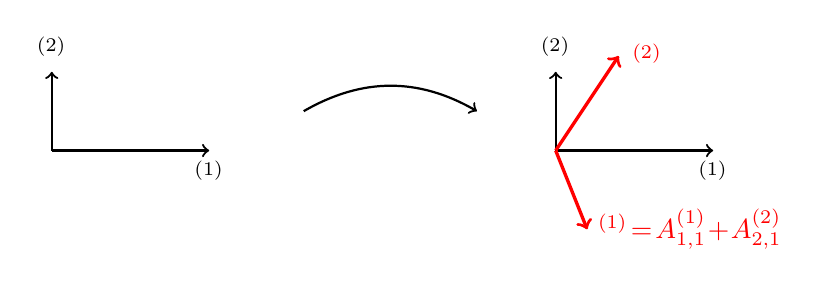
\begin{tikzpicture}[x=2cm]
                % LEFT: Standard basis vectors and unit square
                \begin{scope}
                    \draw[->, thick] (0,0) -- (1,0) node[below] {$\vu^{(1)}$};
                    \draw[->, thick] (0,0) -- (0,1) node[above] {$\vu^{(2)}$};
                \end{scope}
                % RIGHT: Transformed basis vectors and parallelogram
                \begin{scope}[shift={(3.2,0)}]
                    \draw[->, thick] (0,0) -- (1,0) node[below] {$\vv^{(1)}$};
                    \draw[->, thick] (0,0) -- (0,1) node[above] {$\vv^{(2)}$};
                    \coordinate (A) at (0.2,-1.0);
                    \coordinate (B) at (0.4,1.2);
                    \draw[->, very thick, red] (0,0) -- (A) node[below,right] {$\mA \vu^{(1)}\!=\!A_{1,1}\vv^{(1)}\!+\!A_{2,1}\vv^{(2)}$};
                    \draw[->, very thick, red] (0,0) -- (B) node[right,xshift=1pt] {$\mA \vu^{(2)}$};
                \end{scope}
                % Arrow between plots
                \draw[->, thick] (1.6,0.5) to[bend left] node[midway, above] {$\mA$} (2.7,0.5);
            \end{tikzpicture}
        \end{center}
        \caption{Una matriz $\mA$ define una aplicacion lineal entre dos espacios vectoriales} 
        \end{figure}
        Véa también: \gls{linearmap}, \gls{dataset}, \gls{linmodel}, \glspl{modelparam}, \gls{linreg}, \gls{vectorspace} },
    first={matriz},
    firstplural={matrices},
	type=math,
    plural={matrices},
    text={matriz}
}

\newglossaryentry{det}
{name={determinante},
description={El\index{determinante} determinante $\det(\mA)$ de una matriz cuadrada 
$\mA = \big( \va^{(1)},\ldots, \va^{(\nrfeatures)} \big) \in \mathbb{R}^{\nrfeatures \times \nrfeatures}$ 
es una funcion de sus columnas $\va^{(1)},\ldots,\va^{(\nrfeatures)} \in \mathbb{R}^{\nrfeatures}$, que satisface \cite{DirschmidHansJorg1996TuF}
\begin{itemize}
	\item Normalización: $$\det (\mI) = 1$$ 
	\item Multilinealidad: 
	\begin{align} \nonumber 
	\det \big(\va^{(1)},\ldots,\alpha\vu+ \beta \vv,\ldots,\va^{(\nrfeatures)} \big) & = \alpha\det \big(\va^{(1)},\ldots,\vu,\ldots,\va^{(\nrfeatures)} \big) \\ 
	& +\beta\det \big(\va^{(1)},\ldots,\vv,\ldots,\va^{(\nrfeatures)} \big) \nonumber
	\end{align}
	\item Antisimetría: $$\det \big(\ldots,\va^{(\featureidx)}, \ldots, \va^{(\featureidx')},\ldots \big) = - \det \big(\ldots,\va^{(\featureidx')}, \ldots, \va^{(\featureidx)},\ldots \big).$$ 
\end{itemize} 
Podemos interpretar una matriz $\mA$ como una transformación lineal en $\mathbb{R}^{\nrfeatures}$. 
El determinante $\det(\mA)$ caracteriza cómo (y en qué orientación) se alteran los volúmenes en $\mathbb{R}^\nrfeatures$ por esta transformación \cite{GolubVanLoanBook}, \cite{Strang2007}. 
En particular, $\det(\mA) > 0$ preserva la orientación, $\det(\mA) < 0$ la invierte, 
y $\det(\mA) = 0$ colapsa el volumen completamente, lo que indica que $\mA$ no es invertible. 
El determinante también satisface $\det(\mA \mB) = \det(\mA) \cdot \det(\mB)$, y si $\mA$ es 
diagonalizable con valor propio $\eigval{1}, \ldots, \eigval{\nrfeatures}$, entonces 
$\det(\mA) = \prod_{\featureidx=1}^{\nrfeatures} \eigval{\featureidx}$ \cite{HornMatAnalysis}. 
Para los casos especiales $\nrfeatures=2$ (2D) y $\nrfeatures=3$ (3D), el determinante puede interpretarse 
como un área o volumen orientado definido por los vectores columna de $\mA$.
\begin{figure}[H]
	\begin{center}
	\begin{tikzpicture}[x=2cm]
	% LEFT: Standard basis vectors and unit square
	\begin{scope}
	\draw[->, thick] (0,0) -- (1,0) node[below right] {$\vx$};
	\draw[->, thick] (0,0) -- (0,1) node[above left] {$\vy$};
	\end{scope}
	% RIGHT: Transformed basis vectors and parallelogram
	\begin{scope}[shift={(2.8,0)}]
	\coordinate (A) at (1.5,0.5);
	\coordinate (B) at (-0.2,1.2);
	\draw[->, very thick, red] (0,0) -- (A) node[below right] {$\mA \vx$};
	\draw[->, very thick, red] (0,0) -- (B) node[above left] {$\mA \vy$};
	\draw[fill=red!20, opacity=0.6] (0,0) -- (A) -- ($(A)+(B)$) -- (B) -- cycle;
	\draw[dashed] (A) -- ($(A)+(B)$);
	\draw[dashed] (B) -- ($(A)+(B)$);
	\node at (0.8,0.6) {\small $\det(\mA)$};
	\draw[->, thick, blue] (0.4,0.0) arc[start angle=0, end angle=35, radius=0.6];
	\end{scope}
	% Arrow between plots
	\draw[->, thick] (1.3,0.5) -- (2.4,0.5) node[midway, above] {$\mA$};
	\end{tikzpicture}
	\end{center}
	\caption{Podemos interpretar una matriz cuadrada $\mA$ como una transformación lineal de $\mathbb{R}^{\nrfeatures}$ en sí misma. 
	El determinante $\det(\mA)$ caracteriza cómo esta transformación altera un volumen orientado.} 
\end{figure}
Vea tambien: \gls{eigenvalue}, \gls{inverse}.},
first={determinante},
type=math,
text={determinante}
}


\newglossaryentry{linearmap}{
	name={aplicación lineal},
	description={Una\index{aplicación lineal} aplicación lineal $f: \mathbb{R}^n \rightarrow \mathbb{R}^m$ 
		es una función que satisface las propiedades de aditividad: 
		$f(\vx + \vy) = f(\vx) + f(\vy)$, y homogeneidad: 
		$f(c\vx) = c f(\vx)$ para todos los vectores $\vx, \vy \in \mathbb{R}^n$ y escalares $c \in \mathbb{R}$. 
		En particular, $f(\mathbf{0}) = \mathbf{0}$. Toda aplicación lineal puede representarse 
		como una multiplicación matricial $f(\vx) = \mA \vx$ para alguna matriz 
		$\mA \in \mathbb{R}^{m \times n}$. 
		El conjunto de aplicaciones lineales con valores reales para una dimensión $n$ dada constituye un 
		modelo lineal, el cual se utiliza en muchos métodos de aprendizaje automático. \\
		Véa también: \gls{linmodel}, \gls{linreg}, \gls{pca}, \gls{featurevec}.},
	first={aplicación lineal},
	text={aplicación lineal}
}

\newglossaryentry{vector}
{name={vector},
	description={
		Un \index{vector} vector es un elemento de un espacio vectorial. 
		En el contexto del aprendizaje automático, un ejemplo particularmente importante de espacios vectoriales 
		es el espacio euclidiano $\mathbb{R}^{\nrfeatures}$, donde $\nrfeatures \in \mathbb{N}$ 
		representa la dimensión (finita) del espacio. Un vector $\vx \in \mathbb{R}^{\nrfeatures}$ 
		puede representarse como una lista o arreglo unidimensional de números reales, es decir, 
		$x_1, \ldots, x_{\nrfeatures}$ con $x_\featureidx \in \mathbb{R}$ para 
		$\featureidx = 1, \ldots, \nrfeatures$. El valor $x_\featureidx$ es la $\featureidx$-ésima 
		entrada del vector $\vx$. También puede ser útil considerar un vector $\vx \in \mathbb{R}^{\nrfeatures}$ 
		como una función que asigna a cada índice $\featureidx \in \{1, \ldots, \nrfeatures\}$ 
		un valor $x_\featureidx \in \mathbb{R}$, es decir, $\vx: \featureidx \mapsto x_\featureidx$. 
		Esta perspectiva resulta particularmente útil en el estudio de los metodos de kernel.
\begin{figure}[H]
% Left: Stem plot
\begin{minipage}[c]{0.48\textwidth}
\centering 
2,-1,3,0,-2,1
\end{minipage}
\hfill
% Right: Column vector
\begin{minipage}{0.48\textwidth}
\centering
\begin{tikzpicture}
\begin{axis}[
    width=6.5cm,
    height=5cm,
    title={},
    xlabel={index $\featureidx$},
    ylabel={$x_\featureidx$},
    ymin=-3.5, ymax=3.5,
    xmin=0.5, xmax=6.5,
    xtick={1,2,3,4,5,6},
    ytick={-3,-2,-1,0,1,2,3},
    axis x line=bottom,        % <-- horizontal axis at y=0
    axis y line=left,          % <-- vertical axis on the left
    grid=both,
    major grid style={dotted, gray!60},
    enlargelimits=0.1
]
\addplot+[ycomb, thick, mark=*]
    coordinates {
        (1,2)
        (2,-1)
        (3,3)
        (4,0)
        (5,-2)
        (6,1)
    };
\end{axis}
\end{tikzpicture}
\end{minipage}
\caption{Dos representaciones equivalentes de un vector $\vx= \big( 2,-1,3,0,-2,1 \big)^{T} \in \mathbb{R}^{6}$
: como un arreglo numérico (izquierda) y como una función $\featureidx \mapsto x_\featureidx$ (derecha).}
\label{fig:vector-function-dual_dict}
\end{figure}
		Vea tambien: \gls{euclidspace}, \gls{vectorspace}, \gls{linearmap}, \gls{function}, \glspl{kernelmethod}},
	first={vector},
	type=math,
	text={vector}
}

\newglossaryentry{vectorspace}
{
  name={espacio vectorial},
  description={Un \index{espacio vectorial} espacio vectorial $\mathcal{V}$ (también llamado espacio lineal) 
  es una colección de elementos, llamados vectores, junto con las siguientes dos operaciones: 
    1) suma (denotada $\vv+\vw$) de dos vectores $\vv,\vw$; y 2) multiplicación 
    (denotada $c \,\cdot \,\vv$) de un vector $\vv$ con un escalar $c$ que pertenece a algún 
    campo numérico (con una elección típica para este campo siendo $\mathbb{R}$). La propiedad 
    definitoria de un espacio vectorial es que está cerrado bajo estas operaciones:
    \begin{itemize}
      \item Si $\vv, \vw \in \mathcal{V}$, entonces $\vv + \vw \in \mathcal{V}$.
      \item Si $\vv \in \mathcal{V}$ y $c \in \mathbb{R}$, entonces $c \vv \in \mathcal{V}$.
      \item En particular, $\mathbf{0} \in \mathcal{V}$.
    \end{itemize}
    \begin{figure}[H]
    \centering
      \begin{tikzpicture}[>=Stealth, scale=1.2]
        % Coordinates
        \coordinate (O) at (0,0);            % Origin
        \coordinate (V) at (2,1.5);          % vector v
        \coordinate (W) at (1,3);            % vector w
        \coordinate (VplusW) at (3,4.5);     % v + w
        \coordinate (HalfV) at (1,0.75);     % 0.5 * v
        \draw[->, thick, blue] (O) -- (V) node[pos=1, right] {$\vv$};
        \draw[->, thick, red] (O) -- (W) node[pos=1, left] {$\vw$};
        \draw[->, thick, purple] (O) -- (VplusW) node[pos=0.99, above right] {$\vv+\vw$};
        \draw[dashed, red] (V) -- (VplusW);
        \draw[dashed, blue] (W) -- (VplusW);
        \draw[->, thick, orange] (O) -- (HalfV) node[midway, right] {$ \alpha \vv$};
        % Filled dots
        \filldraw[black] (O) circle (2pt) node[below left] {$\mathbf{0}$};  % origin
        \filldraw[blue] (V) circle (2pt);         % v
        \filldraw[red] (W) circle (2pt);          % w
        \filldraw[purple] (VplusW) circle (2pt);  % v + w
        \filldraw[orange] (HalfV) circle (2pt);   % 0.5v
      \end{tikzpicture}
      \caption{Un espacio vectorial $\mathcal{V}$ es una colección de vectores tal que 
      escalar y sumar estos siempre produce otro vector en $\mathcal{V}$.}
      \label{fig:vector-ops_dict}
    \end{figure}
    Un ejemplo común de un espacio vectorial es el espacio euclidiano $\mathbb{R}^n$, que es 
    ampliamente utilizado en aprendizaje automático para representar conjuntos de datos. También podemos usar $\mathbb{R}^n$ 
    para representar, ya sea exactamente o aproximadamente, el espacio de hipótesis utilizado por un método de aprendizaje automático. 
    Otro ejemplo de un espacio vectorial, que está naturalmente asociado con cada espacio de probabilidad
    $\mathcal{P}=\big(\Omega,\mathcal{R},\prob{\cdot} \big)$, es la colección de todas 
    las variables aleatorias con valores reales $x: \Omega \rightarrow \mathbb{R}$ \cite{RudinBook}, \cite{folland1999real}.  
    \\
    Véa también: \gls{vector}, \gls{euclidspace}, \gls{linmodel}, \gls{linearmap}.},
  first={espacio vectorial},
  type=math,
  text={espacio vectorial}
}


\newglossaryentry{stochastic}
{name={estocástico},
	description={Un proceso\index{estocástico} o método se denomina estocástico si implica 
		un componente aleatorio o está regido por leyes probabilísticas. En aprendizaje automático, los métodos 
		estocásticos a menudo incorporan aleatoriedad por razones como la optimización (por ejemplo, 
		descenso por gradiento estocástico) o la modelización de la incertidumbre (por ejemplo, mediante 
		un modelo de probabilidad). Un proceso estocástico es una colección de variables aleatorias indexadas por tiempo 
		o espacio, que se utilizan para modelar fenómenos aleatorios que evolucionan en el tiempo 
		(p. ej., ruido en sensores o series temporales financieras).\\
		Véa también: \gls{ml}, \gls{stochGD}, \gls{uncertainty}, \gls{probmodel}, \gls{rv}, \gls{sbm}.},
	first={estocástico},
	text={estocástico}
}

\newglossaryentry{stochproc}
{name={proceso estocástico},
	description={Un proceso estocástico es una colección de variables aleatorias definidas sobre un mismo espacio de probabilidad. 
		Estas variables aleatorias están indexadas por el tiempo o el espacio, y se utilizan para modelar fenómenos aleatorios
		que evolucionan en el tiempo (por ejemplo, ruido en sensores o series temporales financieras). 
		Grafos aleatorios, como el modelo estocástico de bloques (SBM) o el grafo de Erd, son otro ejemplo de procesos estocásticos. 
		Estos procesos utilizan pares de nodos en un grafo como conjunto de índices. 
		También podemos usar procesos estocásticos para representar algoritmo estocástico como descenso por gradiente estocástico.
		\\
		Véa también: \gls{stochGD}, \gls{uncertainty}, \gls{probmodel}, \gls{rv}, \gls{sbm}.},
	first={proceso estocástico},
	type=math,
	text={proceso estocástico}
}


\newglossaryentry{characteristicfunc}
{name={función característica},
	description={La función característica\index{función característica} 
		de una \gls{rv} real $x$ es la función \cite[Sección 26]{BillingsleyProbMeasure}
		$$ \phi_{x}(t) \defeq \expect { \exp(j t x) } \mbox{ con } j = \sqrt{-1}.$$
	 La función característica determina de forma única la \gls{probdist} de $x$. 
		\\
		Véa también: \gls{probdist}, \gls{rv}.},
	first={función característica},
	type=math,
	text={función característica}
}



\newglossaryentry{entropy}
{name={entropía},
	description={La entropía cuantifica la incertidumbre o imprevisibilidad asociada a una variable aleatoria\cite{coverthomas}. 
		Para una variable aleatoria discreta $x$ que toma valores en un conjunto finito 
		$\mathcal{S} = \{x_1, \ldots, x_n\}$ con función de masa de probabilidad 
		$p_i \defeq \prob{x = x_i}$, la entropía se define como
		\[
		H(x) \defeq -\sum_{i=1}^n p_i \log p_i.
		\]
		La entropía se maximiza cuando todos los resultados son igualmente probables, y se minimiza 
		(es decir, es cero) cuando el resultado es determinista. Una generalización del concepto 
		de entropía para variables aleatorias continuas es la entropía diferencial.\\
		Véa también: \gls{uncertainty}, \gls{probmodel}.},
	first={entropía},
	text={entropía}
}

\newglossaryentry{diffentropy}
{name={entropía diferencial},
	description={Para\index{entropía diferencial} una variable aleatoria con valores reales $\featurevec \in \mathbb{R}^{\nrfeatures}$ 
		con función de densidad de probabilidad $p(x)$, la entropía diferencial se define como \cite{coverthomas}
		\[
		h(\featurevec) \defeq - \int p(\featurevec) \log p(\featurevec) \, d\featurevec.
		\]
		La entropía diferencial puede ser negativa y carece de algunas propiedades de la entropía 
		para variables aleatorias discretas, como la invariancia ante cambios de variable \cite{coverthomas}. 
		Entre todas las variables aleatorias con media $\meanvecgeneric$ y matriz de covarianza $\covmtxgeneric$ dadas, 
		$h(\featurevec)$ se maximiza cuando $\featurevec \sim \mvnormal{\meanvecgeneric}{\covmtxgeneric}$. \\
		Véa también: \gls{rv}, \gls{pdf}, \gls{mean}, \gls{covmtx}, \gls{uncertainty}, \gls{probmodel}.},
	first={entropía diferencial},
	text={entropía diferencial}
}


\newglossaryentry{minimum}
{
	name=mínimo,
	description={Dado un conjunto de números reales, el mínimo\index{mínimo} es el menor de esos números.},
	first={mínimo},text={mínimo}
}

\newglossaryentry{function}
{name={función},
	description={
		Una función\index{función} entre dos conjuntos $\mathcal{U}$ y $\mathcal{V}$ 
	asigna a cada elemento $u \in \mathcal{U}$ exactamente un elemento $v \in \mathcal{V}$  \cite{RudinBookPrinciplesMatheAnalysis}. 
		Esto se escribe como $f: \mathcal{U} \rightarrow \mathcal{V}$, donde $\mathcal{U}$ es el dominio 
		y $\mathcal{V}$ el codominio de $f$. Es decir, una función $f$ define una salida única 
		$f(u) \in \mathcal{V}$ para cada entrada $u \in \mathcal{U}$ (see Fig. \ref{fig_function_dict}).
		\begin{figure}[H]
			\centering
			\begin{tikzpicture}[>=stealth, node distance=1.2cm and 2.5cm]
				\tikzset{dot/.style={circle, fill=black, inner sep=1.2pt}}
				\node (A) [dot, label=left:$a$] {};
				\node (B) [dot, below=of A, label=left:$b$] {};
				\node (C) [dot, below=of B, label=left:$c$] {};
				\node (1) [dot, right=4cm of A, label=right:$1$] {};
				\node (2) [dot, below=of 1, label=right:$2$] {};
				\node (3) [dot, below=of 2, label=right:$3$] {};
				\node[draw=blue!70, thick, ellipse, inner sep=0.5cm, fit=(A)(B)(C), label=above:$\mathcal{U}$] {};
				\node[draw=green!70!black, thick, ellipse, inner sep=0.5cm, fit=(1)(2)(3), label=above:$\mathcal{V}$] {};
				\draw[->] (A) -- (2);
				\draw[->] (B) -- (1);
				\draw[->] (C) -- (2);
			\end{tikzpicture}
			\caption{Una función \( f \colon \{a,b,c\} \to \{1,2,3\} \) mapea cada elemento del dominio a exactamente un elemento del 
				codominio. \label{fig_function_dict}}
		\end{figure} },
	first={función},
	type=math,
	text={función}
}



\newglossaryentry{map}
{name={aplicación}, 
	description={Utilizamos el término aplicación\index{aplicación} como sinónimo de función.\\
	Véa también: \gls{function}.
	},
	first={aplicación},
	type=math,
	text={aplicación}
}


\newglossaryentry{attention}{
name={atención},
description={
Algunas aplicaciones de aprendizaje automático\index{atención} implican puntos de datos compuestos por unidades más pequeñas, conocidas 
como *tokens*. Por ejemplo, una oración se compone de palabras, una imagen de parches de píxeles y una red de 
nodos. En la práctica, los tokens dentro de un solo punto de datos típicamente no son independientes entre sí, 
sino que cada token presta atención a ciertos otros tokens. Los modelos de probabilidad proporcionan un marco 
fundamentado para representar y analizar tales dependencias \cite{Blei2003}. Los mecanismos de atención utilizan 
un enfoque más directo, sin referencia explícita a un modelo de probabilidad. La idea es representar la relación entre dos 
tokens $\nodeidx$ y $\nodeidx'$ mediante una funcion parametrizada $f^{(\weights)}(\nodeidx,\nodeidx')$, 
donde los parametros $\weights$ se aprenden mediante una variante de ERM. 
Los mecanismos de atención prácticos difieren tanto en la elección precisa del modelo de atención 
$f^{(\weights)}(\nodeidx,\nodeidx')$ como en la variante específica de ERM empleada para aprender 
los parametros $\weights$. Una familia ampliamente utilizada de mecanismos de atención define los parámetros 
$\weights$ en términos de dos vectores asociados a cada token $\nodeidx$: un vector de consulta 
$\vq^{(\nodeidx)}$ y un vector clave $\vk^{(\nodeidx')}$. Para un token dado $\nodeidx$ con consulta 
$\vq^{(\nodeidx)}$ y otro token $\nodeidx'$ con clave $\vk^{(\nodeidx')}$, la cantidad 
$\big( \vq^{(\nodeidx)} \big)^{\top} \vk^{(\nodeidx')}$ cuantifica hasta qué punto el token $\nodeidx$ presta atención 
a (o depende de) $\nodeidx'$.
\begin{figure}[H]
	\centering
	\begin{tikzpicture}[>=stealth, node distance=0.2cm and 0.2cm,
		every node/.style={inner sep=2pt, font=\large}, baseline]
		% Words (sentence: All human beings are born free and equal.)
		\node (w1) [draw, fill=gray!10, rounded corners] {All};
		\node (w2) [draw, fill=gray!10, right=of w1, rounded corners] {human};
		\node (w3) [draw, fill=gray!10, right=of w2, rounded corners] {beings};
		\node (w4) [draw, fill=gray!10, right=of w3, rounded corners] {are};
		\node (w5) [draw, fill=gray!10, right=of w4, rounded corners] {born};
		\node (w6) [draw, fill=gray!10, right=of w5, rounded corners] {free};
		\node (w7) [draw, fill=gray!10, right=of w6, rounded corners] {and};
		\node (w8) [draw, fill=blue!20, right=of w7, rounded corners] {equal};
	% Label "i" below the word "equal"
   	   		\node[font=\footnotesize, below=0.15cm of w8, align=center] (labeli) {$\nodeidx$ \\ $\vq^{(\nodeidx)},\ \vk^{(\nodeidx)}$};
		\node[font=\footnotesize, below=0.15cm of w1, align=center] (labelii) {$\nodeidx'$ \\ $\vq^{(\nodeidx')},\ \vk^{(\nodeidx')}$};
	% Dummy node above for routing attention arrows
	  \node (eqTop) [above=1.8cm of w8] {};
	% Arrows from "equal" to earlier words (drawn above)
	 \draw[->, thick, opacity=0.3] (w8.north) .. controls +(up:1.0cm) and +(up:1.0cm) .. (w6.north); % hacia "free"
	 \draw[->, thick, opacity=0.3] (w8.north) .. controls +(up:1.2cm) and +(up:1.0cm) .. (w5.north); % hacia "born"
	 \draw[->, thick, opacity=1]  (w8.north)  .. controls +(up:1.8cm) and +(up:1.0cm) ..  
	 	node[midway, text=black, above] {$f^{(\weights)}(\nodeidx,\nodeidx')$}  (w1.north); % hacia "All"
	\end{tikzpicture}
	\caption{Los mecanismos de atención aprenden una función parametrizada $f^{(\weights)}(\nodeidx,\nodeidx')$ que mide 
	cuánto atención presta el token $\nodeidx$ al token $\nodeidx'$. Una construcción ampliamente utilizada de 
	$f^{(\weights)}(\nodeidx,\nodeidx')$ emplea vectores de consulta y clave, $\vq^{(\nodeidx)}$ y $\vk^{(\nodeidx)}$, 
	asignados a cada token $\nodeidx$ \cite{vaswani2017attention}.}
\end{figure}
Véa también: \gls{function}.},
first={atención},
text={atención}
}




\newglossaryentry{optproblem}
{name={problema de optimización},
	description={
		Un\index{problema de optimización} problema de optimización es una estructura matemática 
		que consiste en una función objetivo $f: \mathcal{U} \rightarrow \mathcal{V}$ definida 
		sobre una variable de optimización $\weights \in \mathcal{U}$, junto con un conjunto factible 
		$\mathcal{W} \subseteq \mathcal{U}$. Se asume que el codominio $\mathcal{V}$ está ordenado, 
		lo que significa que para cualesquiera dos elementos $\mathbf{a}, \mathbf{b} \in \mathcal{V}$, 
		podemos determinar si $\mathbf{a} < \mathbf{b}$, $\mathbf{a} = \mathbf{b}$ o 
		$\mathbf{a} > \mathbf{b}$. El objetivo de la optimización es encontrar aquellos valores 
		$\weights \in \mathcal{W}$ para los cuales el valor de la función objetivo $f(\weights)$ 
		es extremo —es decir, mínimo o máximo \cite{BoydConvexBook,nesterov04,BertsekasNonLinProgr}.
	},
	first={problema de optimización},
	type=math,
	text={problema de optimización}
}





\newglossaryentry{optmethod}
{name={método de optimización},
	description={Un\index{método de optimización} método de optimización es un \gls{algorithm} 
		que recibe como entrada una representación de un problema de optimización y entrega como salida 
		una solución (aproximada) \cite{BoydConvexBook}, \cite{nesterov04}, \cite{BertsekasNonLinProgr}.\\
		Véa también: \gls{algorithm}, \gls{optproblem}.
	},
	first={método de optimización},
	text={método de optimización}
}

% \newglossaryentry{fixedpointiter}
% {name={méthode du point fixe},
% 	description={La \index{méthode du point fixe} méthode du point fixe est une méthode itérative 
% 		permettant de résoudre un \gls{optproblem}. Elle construit une suite \( \weights^{(0)}, \weights^{(1)}, \ldots \) 
% 		en appliquant de manière répétée un opérateur \( \fixedpointop \), c’est-à-dire:
% 		\begin{equation} 
% 			\label{equ_def_fixed_point_dict} 
% 			\weights^{(\iteridx+1)} = \fixedpointop \weights^{(\iteridx)}, \quad \text{pour } \iteridx = 0, 1, \ldots.
% 		\end{equation} 
% 		L’opérateur \( \fixedpointop \) est choisi de sorte que tout point fixe soit une solution 
% 		\( \widehat{\weights} \) du \gls{optproblem} donné. Par exemple, étant donnée une \gls{function} \( f(\weights) \) \gls{convex} et 
% 		\gls{diffentropy}, les points fixes de l’opérateur 
% 		\( \fixedpointop: \weights \mapsto \weights - \nabla f(\weights) \) coïncident avec les minimiseurs de \( f(\weights) \).
% 		De manière générale, pour un problème d’optimisation donné dont la solution est \( \widehat{\weights} \), 
% 		il peut exister plusieurs opérateurs \( \fixedpointop \) ayant pour points fixes \( \widehat{\weights} \). 
% 		Il est donc clairement souhaitable d’utiliser un opérateur \( \fixedpointop \) tel que l’itération 
% 		\eqref{equ_def_fixed_point_dict} réduise la distance à la solution :
% 		\begin{equation}
% 			\nonumber
% 			\underbrace{\normgeneric{ \weights^{(\iteridx+1)} - \widehat{\netparams}}{2}}_{\stackrel{\eqref{equ_def_fixed_point_dict}}{=} 
% 				\normgeneric{ \fixedpointop \weights^{(\iteridx)} - \fixedpointop\widehat{\weights}}{2}}  \leq 
% 			\normgeneric{ \weights^{(\iteridx)} - \widehat{\weights}}{2}.
% 		\end{equation}
% 		On exige donc que \( \fixedpointop \) soit au minimum non-expansif, c’est-à-dire que l’itération 
% 		\eqref{equ_def_fixed_point_dict} ne produise pas des \glspl{modelparam} plus éloignés de la solution 
% 		\( \widehat{\weights} \).
% 		Mieux encore, chaque itération \eqref{equ_def_fixed_point_dict} devrait faire progresser la solution, 
% 		en réduisant effectivement la distance à \( \widehat{\weights} \). Cette exigence peut être formulée 
% 		précisément à l’aide de la notion d’\gls{contractop} \cite{Bauschke:2017}, \cite{fixedpoinIsta}. 
% 		On dit que \( \fixedpointop \) est un \gls{contractop} s’il existe un facteur \( \contractfac \in [0,1) \) tel que
% 		\begin{equation}
% 			\nonumber
% 			\normgeneric{ \fixedpointop \weights - \fixedpointop \weights'}{2}  \leq  \contractfac \normgeneric{\weights - \weights'}{2} 
% 			\quad \text{pour tout } \weights, \weights'.
% 		\end{equation}
% 		Avec un \gls{contractop} \( \fixedpointop \), l’itération \eqref{equ_def_fixed_point_dict} 
% 		génère une suite \( \weights^{(\iteridx)} \) qui converge rapidement. En particulier \cite[Th. 9.23]{RudinBookPrinciplesMatheAnalysis}, on a:
% 		\begin{equation}
% 			\nonumber
% 			\normgeneric{ \weights^{(\iteridx)} - \widehat{\weights}}{2} \leq \contractfac^{\iteridx} 
% 			\normgeneric{ \weights^{(0)} - \widehat{\weights}}{2}.
% 		\end{equation}
% 		Ici, \( \normgeneric{ \weights^{(0)} - \widehat{\weights}}{2} \) est la distance entre l’initialisation 
% 		et la solution.
% 		Il s’avère que la méthode du point fixe \eqref{equ_def_fixed_point_dict} utilisant un opérateur 
% 		ferme non-expansif \( \fixedpointop \) est garantie de converger vers un point fixe de \( \fixedpointop \) 
% 		\cite[Cor. 5.16]{Bauschke:2017}. La Fig.~\ref{fig_examples_nonexp_dict} montre des exemples d’un opérateur 
% 		ferme non-expansif, d’un opérateur non-expansif, et d’un \gls{contractop}, tous définis sur \( \mathbb{R} \).		
% 		Un autre exemple d’opérateur ferme non-expansif est l’\gls{proxop} d’une \gls{function} \gls{convex} 
% 		\cite{Bauschke:2017}, \cite{ProximalMethods}. 
% 		\definecolor{darkgreen}{rgb}{0.0, 0.5, 0.0}
% 		\begin{figure}[H]
% 			\begin{center} 
% 				\begin{tikzpicture}[scale=1.5]
% 					% Axes
% 					\draw[line width=1pt, ->] (-2,0) -- (2,0) node[right] {$\weight^{(\iteridx)}$};
% 					\draw[line width=1pt, ->] (0,-2) -- (0,2) node[above] {$\weight^{(\iteridx+1)}$};
% 					% Labels
% 					\node at (2.1,2.2) {$\fixedpointop^{(3)}$};
% 					\node at (1.9,-1.5) {$\fixedpointop^{(1)}$};
% 					\node at (1.5,1.2) {$\fixedpointop^{(2)}$};
% 					% Dashed lines at x=1 and y=1
% 					\draw[dashed] (1,-2) -- (1,2); % Vertical line at x=1
% 					\draw[dashed] (-2,1) -- (2,1); % Horizontal line at y=1
% 					\draw[dashed] (-2,-1) -- (2,-1); % Horizontal line at y=1
% 					\draw[dashed] (-1,-2) -- (-1,2); % Vertical line at x=1
% 					\node[above,xshift=4pt,yshift=-1pt] at (1,0) {$1$};
% 					\node[above,xshift=8pt,yshift=-1pt] at (0,-1) {$-1$};
% 					% First curve: y = 1/2 x + 1
% 					\draw[line width=2,domain=-2:2,smooth,blue] plot(\x,{0.5*\x + 1});
% 					% Second curve: y = -x
% 					\draw[line width=2,domain=-2:2,smooth,red] plot(\x,{-\x});
% 					% Third curve: y = x / |x| * min(|x|, 1)
% 					\draw[line width=2, domain=-2:-1,smooth,darkgreen] plot(\x,{-1});
% 					\draw[line width=2,domain=-1:1,smooth,darkgreen] plot(\x,{\x});
% 					\draw[line width=2,domain=1:2,smooth,darkgreen] plot(\x,{1});
% 				\end{tikzpicture}
% 			\end{center} 
% 			\caption{Exemple d'opérateur non-expansif $\fixedpointop^{(1)}$, opérateur ferme non-expansif $\fixedpointop^{(2)}$, et \gls{contractop} $\fixedpointop^{(3)}$. \label{fig_examples_nonexp_dict}}
% 		\end{figure}
% 		Voir aussi: \gls{optproblem}, \gls{differentiable}, \gls{convex} \gls{function}, \glspl{modelparam}, 
% 		\gls{contractop}, \gls{proxop}.},
% 	first={méthode du point fixe},
% 	text={méthode du point fixe},
% 	plural={méthodes du point fixe}
% }


\newglossaryentry{ergraph}
{name={grafo de Erd\H{o}s-R\'enyi (grafo ER)},
	description={Un grafo ER es un modelo de probabilidad para grafos definido sobre 
		un conjunto dado de nodos $\nodeidx=1,\ldots,\nrnodes$. Una forma de definir el 
		grafo ER es mediante una colección de variables aleatorias iid binarias 
		$b^{(\edge{\nodeidx}{\nodeidx'})} \in \{0,1\}$, para cada par de nodos distintos 
		$\nodeidx, \nodeidx'$. Una realización específica del grafo ER contiene 
		una arista $\edge{\nodeidx}{\nodeidx'}$ si y solo si 
		$b^{(\edge{\nodeidx}{\nodeidx'})}=1$. El grafo ER está parametrizado por el 
		número $\nrnodes$ de nodos y la probabilidad
		$\prob{b^{(\edge{\nodeidx}{\nodeidx'})}=1}$.\\
		Véa también: \gls{graph}, \gls{probmodel}, \gls{iid}, \gls{rv}, \gls{realization}, \gls{probability}.
	},
	first={grafo de Erd\H{o}s-R\'enyi (grafo ER)},
	text={grafo ER}
}


\newglossaryentry{attack}
{name={ataque},  
	description={Un ataque\index{ataque} a un sistema de aprendizaje automático se refiere a una acción intencional—ya sea 
		activa o pasiva—que compromete la integridad, disponibilidad o confidencialidad del sistema. 
		Los ataques activos implican la alteración de componentes como los conjuntos de datos
		(por medio de envenenamiento de datos) o de los enlaces de comunicación entre dispositivos 
		en un entorno de aprendizaje federado. Los ataques pasivos, como los ataques a la privacidad, 
		buscan inferir atributos sensibles sin modificar el sistema. 
		Según su objetivo, distinguimos entre ataques de denegación de servicio, ataques de puerta trasera y ataques a la privacidad.\\
		Véa también: \gls{datapoisoning}, \gls{privattack}, \gls{sensattr}, \gls{dosattack}, \gls{backdoor}.}, 
	first={ataque},
	text={ataque}
}



\newglossaryentry{privattack}
{name={ataque a la privacidad},
	description={Un ataque\index{ataque a la privacidad} a la privacidad en un sistema de aprendizaje automático
		tiene como objetivo inferir atributos sensibles de individuos mediante el aprovechamiento 
		del acceso parcial a un modelo de aprendizaje automático ya entrenado. 
		Una forma de ataque a la privacidad es la inversion de modelo.\\
		Véa también: \gls{attack}, \gls{ml}, \gls{sensattr}, \gls{modelinversion}, \gls{trustAI}, \gls{gdpr}.
	},
	first={ataque a la privacidad}, 
	text={ataque a la privacidad}
}


\newglossaryentry{epigraph}
{name={epígrafo},
  description={El epígrafo\index{epígrafo} de una función real 
  $f : \mathbb{R}^n \to \mathbb{R} \cup \{+\infty\}$ es el conjunto de puntos que 
  se encuentran sobre o en el grafo de la función:
	\[
	\operatorname{epi}(f) = \left\{ (\mathbf{x}, t) \in \mathbb{R}^n \times \mathbb{R} \,\middle|\, f(\mathbf{x}) \leq t \right\}.
	\]
	Una funcion es convexa si y solo si su epígrafo es un conjunto convexo
	\cite{BoydConvexBook}, \cite{BertCvxAnalOpt}.
	\begin{figure}[H]
		\centering
		\begin{tikzpicture}[scale=1.0]
			\begin{axis}[
				axis lines = middle,
				xlabel = $x$,
				ylabel = {},
				xmin=-2, xmax=2,
				ymin=0, ymax=4.5,
				samples=100,
				domain=-1.5:1.5,
				thick,
				width=8cm,
				height=6cm,
				grid=none,
				axis on top,
				]
				% Function
				\addplot [blue, thick, domain=-1.5:1.5] {x^2} 
					node [pos=0.85, anchor=south west, xshift=5pt] {$f(x)$};
				% Epigraph shading
				\addplot [
					name path=f,
					draw=none,
					ytick=\empty,
					domain=-1.5:1.5,
					] {x^2};
				\path[name path=top] (axis cs:-1.5,4) -- (axis cs:1.5,4);
				\addplot [
					blue!20,
					opacity=0.6,
					draw=none,
					] fill between [
					of=f and top,
					soft clip={domain=-1.5:1.5},
					];
				\node[font=\small] at (axis cs:-1.0,2.3) {$\operatorname{epi} f$};
			\end{axis}
		\end{tikzpicture}
		\caption{Epígrafo de la función $f(x) = x^2$ (área sombreada).}
	\end{figure}
	Véa también: \gls{function}, \gls{graph}, \gls{convex}.
  },
  first={epígrafo},
  text={epígrafo}
}

\newglossaryentry{nullspace}
{name={espacio nulo},
	description={El espacio nulo\index{nullspace} de una matriz $\mA \in \mathbb{R}^{\nrfeatures' \times \nrfeatures}$, 
		denotado como ${\rm null}(\mA)$, es el conjunto de todos los vectores $\mathbf{n} \in \mathbb{R}^\nrfeatures$ 
    		tales que $$\mA \mathbf{n} = \mathbf{0}.$$ 
		Consideremos un método de aprendizaje de atributos que utiliza la matriz $\mA$ para transformar 
		un vector de atributos $\mathbf{x} \in \mathbb{R}^{\nrfeatures}$ de un punto de datos 
		en un nuevo vector de atributos $\vz = \mA \mathbf{x} \in \mathbb{R}^{\nrfeatures'}$. 
		El espacio nulo ${\rm null}(\mA)$ caracteriza todas las direcciones en el 
		espacio de atributos original $\mathbb{R}^{\nrfeatures}$ a lo largo de las cuales la transformación 
		$\mA \mathbf{x}$ permanece invariante. En otras palabras, sumar cualquier vector del 
		espacio nulo a un vector de atributos $\featurevec$ no afecta a la representación transformada $\vz$. 
		Esta propiedad puede explotarse para imponer invariancias en las predicciónes 
		(calculadas a partir de $\mA \mathbf{x}$). La Fig.\ \ref{fig:nullspace-rotation-dict} 
		ilustra una de estas invariancias. Muestra versiones rotadas de dos dígitos manuscritos, 
		que aproximadamente se sitúan a lo largo de curvas unidimensionales en el espacio de atributos original. 
		Estas curvas están alineadas con un vector de dirección $\mathbf{n} \in \mathbb{R}^{\nrfeatures}$. 
    		Para garantizar que el modelo entrenado sea invariante a dichas rotaciones, podemos 
		elegir la matriz de transformación $\mA$ de manera que $\mathbf{n} \in {\rm null}(\mA)$. 
		Esto asegura que $\mA \mathbf{x}$, y por lo tanto la predicción resultante, 
		sea aproximadamente insensible a rotaciones de la imagen de entrada.
		\begin{figure}[H]
      			\centering
      			\includegraphics[width=0.6\textwidth]{../../assets/pythonsnacks/nullspace_0_1.png}
	  		\caption{Imágenes rotadas de dos dígitos manuscritos. Las rotaciones se alinean aproximadamente 
	  		a lo largo de curvas lineales paralelas al vector $\mathbf{n}$.\label{fig:nullspace-rotation-dict}}	
	       	\end{figure}
		Véa también: \gls{matrix}. \\ 
		Demo en Python: \href{https://github.com/AaltoDictionaryofML/AaltoDictionaryofML.github.io/blob/main/assets/pythonsnacks/nullspace.py}{click aquí}},
 	first={espacio nulo},
 	firstplural={espacios nulos},
 	plural={espacios nulos},
 	text={espacio nulo}
}


\newglossaryentry{maximum}
{name=máximo,
 %description={Given a set of real numbers, the maximum\index{maximum} is the largest of those numbers.},
     description={El máximo\index{máximo} de un conjunto $\mathcal{A} \subseteq \mathbb{R}$ 
	 de números reales es el elemento más grande en ese conjunto, si tal elemento existe. Un conjunto $\mathcal{A}$ 
	 tiene un máximo si está acotado superiormente y alcanza su supremo \cite[Sec.~1.4]{RudinBookPrinciplesMatheAnalysis}
	 \\
		Vea también: \gls{supremum}.},
 first={máximo},text={máximo}
}

\newglossaryentry{supremum}
{name=supremo (o mínimo de las cotas superiores),
	description={El supremo\index{supremo (o mínimo de las cotas superiores)} de un conjunto de números reales es 
		el número más pequeño que es mayor o igual que todos los elementos del conjunto. Formalmente, un número real 
		$a$ es el supremo de un conjunto $\mathcal{A} \subseteq \mathbb{R}$ si: 1) $a$ 
		es una cota superior de $\mathcal{A}$; y 2) ningún número menor que $a$ es una cota superior de $\mathcal{A}$. 
		Todo conjunto no vacío de números reales que esté acotado superiormente tiene un supremo,aun si no contiene su supremo como un elemento \cite[Sec.~1.4]{RudinBookPrinciplesMatheAnalysis}.},
	first={supremo (o mínimo de las cotas superiores)},text={supremo}
}

\newglossaryentry{discrepancy}
{name=discrepancia,
	description={
		Considere\index{discrepancia} una aplicacion de aprendizaje federado con datos en red 
		representada por un red FL. Los métodos de aprendizaje federado utilizan una medida de discrepancia para  
		comparar los mapas de hipótesis generados por los modelos locales en los nodos $\nodeidx,\nodeidx'$ 
		conectados por una arista en la red FL.
		\\
			Vea también: \gls{fl}, \gls{netdata}, \gls{empgraph}, \gls{hypothesis}, \gls{localmodel} },
	first={discrepancia},text={discrepancia}
}

\newglossaryentry{FedRelax}
{name={FedRelax},
	description={Un\index{FedRelax} algoritmo distribuido de aprendizaje federado.\\ 
		Véa también: \gls{fl}, \gls{distributedalgorithm}.},
	first={FedRelax},
	text={FedRelax}
} 

\newglossaryentry{fedavg}
{
	name={FedAvg},
	description={FedAvg\index{FedAvg} se refiere a una familia de algoritmos iterativos de aprendizaje federado.
		Utiliza una configuración cliente-servidor y alterna entre el reentrenamiento de modelos locales en los clientes,
		seguido de la agregación de parametros del modelo actualizados en el servidor \cite{pmlr-v54-mcmahan17a}.
		La actualización local en el cliente $\nodeidx=1, \ldots, \nrnodes$ en el tiempo $\iteridx$ comienza con los
		parametros del modelo actuales $\weights^{(\iteridx)}$ proporcionados por el servidor y típicamente consiste en ejecutar
		unas pocas iteraciones de descenso por gradiente estocastico. Tras completar las actualizaciones locales, estas se agregan en el servidor
		(por ejemplo, promediándolas). La Fig. \ref{fig_single_iteration_fedavg_dict} ilustra la ejecución de una sola
		iteración de FedAvg.
		\begin{figure}[H]
			\begin{center}
			\begin{tikzpicture}[>=Stealth, node distance=1cm and 1.5cm, every node/.style={font=\small}]
			% Styles
			\tikzstyle{server} = [circle, fill=black, minimum size=6pt, inner sep=0pt]
			\tikzstyle{client} = [circle, draw=black, minimum size=6pt, inner sep=0pt]
			% Time step labels
			\node (label1) at (0,3.5) {difusión};
			\node[right=2.5cm of label1] (label2) {actualización local};
			\node[right=2.5cm of label2] (label3) {agregación};
			% Time step k
			\node[server] (s1) at (label1 |- 0,2.5) {};
			\node[client] (c1l) at ($(s1) + (-1cm,-1cm)$) {};
			\node[client] (c1r) at ($(s1) + (1cm,-1cm)$) {};
			\node[] (dots1) at ($(s1) + (0cm,-1cm)$) {\ldots};
			\draw[->] (s1) -- (c1l) node[midway,left] {$\weights^{(\iteridx)}$};
			\draw[->] (s1) -- (c1r) node[midway,right] {$\weights^{(\iteridx)}$};
			\draw[->] (s1) -- (dots1);
			% Time step k+1 (local updates)
			\node[server] (s2) at (label2 |- 0,2.5) {};
			\node[client] (c2l) at ($(s2) + (-1cm,-1cm)$) {};
			\node[client] (c2r) at ($(s2) + (1cm,-1cm)$) {};
			\node[] (dots2) at ($(s2) + (0cm,-1cm)$) {\ldots};
			\node[below=0.2cm of c2l] {$\localparamsiter{\iteridx}{1}$};
			\node[below=0.2cm of c2r] {$\localparamsiter{\iteridx}{\nrnodes}$};
			% Time step k+2 (aggregation)
			\node[server] (s3) at (label3 |- 0,2.5) {};
			\node[above=0.01cm of s3, yshift=-4pt] {$\weights^{(\iteridx+1)}$};
			\node[client] (c3l) at ($(s3) + (-1cm,-1cm)$) {};
			\node[client] (c3r) at ($(s3) + (1cm,-1cm)$) {};
			\node[] (dots3) at ($(s3) + (0cm,-1cm)$) {\ldots};
			\draw[->] (c3l) -- (s3) node[midway,left] {$\localparamsiter{\iteridx}{1}$};
			\draw[->] (c3r) -- (s3) node[midway,right] {$\localparamsiter{\iteridx}{\nrnodes}$};
			\draw[->] (dots3) -- (s3);
			\end{tikzpicture}
			\end{center}
			\caption{Ilustración de una sola iteración de FedAvg, que consiste en la difusión de parametros del modelo por parte del
			servidor, la realización de actualizaciones locales en los clientes y la agregación de las actualizaciones por parte del servidor.
			\label{fig_single_iteration_fedavg_dict}}
		\end{figure}
		Véa también: \gls{fl}, \gls{algorithm}, \gls{localmodel}, \gls{stochGD}.},
	first={FedAvg},
	text={FedAvg}
}

\newglossaryentry{FedGD}
{name={FedGD},
	description={Un\index{FedGD} algoritmo distribuido de aprendizaje federado que 
		puede implementarse como paso de mensajes a través de una red de aprendizaje federado.\\ 
		Véa también: \gls{fl}, \gls{distributedalgorithm}, \gls{empgraph}, \gls{gradstep}, \gls{gdmethods}.},
	first={FedGD},
	text={FedGD}
} 

\newglossaryentry{FedSGD}
{name={FedSGD},
	description={Un\index{FedSGD} algoritmo distribuido de aprendizaje federado que 
		puede implementarse como paso de mensajes a través de una red de aprendizaje federado.\\ 
		Véa también: \gls{fl}, \gls{distributedalgorithm}, \gls{empgraph}, \gls{gradstep}, \gls{gdmethods}, \gls{stochGD}.},
	first={FedSGD},
	text={FedSGD}
} 


\newglossaryentry{hfl}
{name={aprendizaje federado horizontal (horizontal FL)},
	description={
		El aprendizaje federado horizontal\index{aprendizaje federado horizontal (horizontal FL)} utiliza conjunto de datos locales constituidos por diferentes
		puntos de datos, pero emplea los mismos atributos para caracterizarlos \cite{HFLChapter2020}.
		Por ejemplo, la predicción meteorológica utiliza una red de estaciones meteorológicas
		(observación) distribuidas espacialmente. Cada estación mide las mismas cantidades, como
		la temperatura diaria, la presión atmosférica y la precipitación. Sin embargo,
		distintas estaciones miden las características o atributos de diferentes regiones espaciotemporales.
		Cada región espaciotemporal representa un punto de datos individual, caracterizado por los los mismos atributos
		(por ejemplo, temperatura diaria o presión atmosférica).
		\\
			Vea también: \gls{localdataset}, \gls{datapoint}, \gls{feature}s },
	first={aprendizaje federado horizontal},text={horizontal FL}
}

\newglossaryentry{dimred}
{name={reducción de dimensionalidad},
	description={La reducción de dimensionalidad\index{reducción de dimensionalidad} se refiere 
		a métodos que aprenden una transformación 
		$\hypothesis: \mathbb{R}^{\nrfeatures} \rightarrow \mathbb{R}^{\nrfeatures'}$ 
		de un conjunto (típicamente grande) de atributos originales 
		$\feature_{1},\ldots,\feature_{\nrfeatures}$ a un conjunto más pequeño de 
		atributos informativas $z_{1},\ldots,z_{\nrfeatures'}$. 
		Usar un conjunto más pequeño de atributos ofrece múltiples ventajas: 
		\begin{itemize} 
			\item \textbf{Ventaja estadística:} Disminuir la cantidad de atributos reduce usualmente 
			la \gls{effdim} de un modelo, lo cual a su vez disminuye el riesgo de sobreajuste.
			\item \textbf{Ventaja computacional:} Menos atributos implican menos carga computacional 
			durante el entrenamiento de los modelos. Por ejemplo, los métodos de regresión lineal 
			requieren invertir una matriz cuyo tamaño depende del número de atributos.
			\item \textbf{Visualización:} La reducción de dimensionalidad es clave para la visualización de datos. 
			Por ejemplo, se puede aprender una transformación que genere dos atributos $z_{1}, z_{2}$ 
			y emplearlas como coordenadas en un diagrama de dispersión. La Figura~\ref{fig:dimred-scatter_dict} 
			ilustra dicho diagrama de dispersión con dígitos manuscritos transformados a partir de imágenes 
			de alta dimensión representadas por valores de escala de grises.
		\end{itemize} 
		 \begin{figure}[H]
		 \centering
		 \begin{tikzpicture}[scale=1]	
		 	% Ejes
		 	\draw[->] (-0.5,0) -- (5.5,0) node[right] {$z_1$};
		 	\draw[->] (0,-0.5) -- (0,4.5) node[above] {$z_2$};
		 	% Puntos de ejemplo con etiquetas
		 	\foreach \x/\y/\label in {
  		 		1.2/0.5/3,
  		 		0.8/2.0/8,
  		 		2.5/1.8/1,
  		 		3.8/3.5/6,
  		 		4.2/0.7/9,
  		 		2.8/3.0/7,
  		 		1.5/3.8/2
		 	}{
  		 		\node[draw, minimum size=0.6cm, inner sep=0pt] at (\x,\y)
    	 		{\label};
		 	}
		 	\end{tikzpicture}
		 	\caption{Ejemplo de reducción de dimensionalidad: Datos de imágenes de alta dimensión 
			(p. ej., dígitos manuscritos) incrustados en 2D mediante atributos aprendidas $(z_1, z_2)$ 
			y visualizados en un diagrama de dispersión.}
		 	\label{fig:dimred-scatter_dict}
		 \end{figure}
		Véa también: \gls{overfitting}, \gls{effdim}, \gls{model}, \gls{scatterplot}.
	}, 
	first={reducción de dimensionalidad},
	text={reducción de dimensionalidad}
}  


\newglossaryentry{ml}
{name={aprendizaje automático (ML)},
	description={\needspace{6\baselineskip}
		El aprendizaje automático\index{aprendizaje automático (ML)} tiene como objetivo predecir
		una etiqueta a partir de los atributos de un punto de datos. Los métodos de ML logran esto
		aprendiendo una hipótesis de un espacio de hipótesis (o modelo)
		mediante la minimización de una función de pérdida \cite{MLBasics,HastieWainwrightBook}.
		Una formulación precisa de este principio es la minimización empírica del riesgo (ERM).
		Diferentes métodos de ML se obtienen de distintas elecciones de diseño para los
		puntos de datos (sus atributos y etiquetas),
		el modelo, y la función de pérdida \cite[Cap. 3]{MLBasics}.
		\\
		Vea también: \gls{label}, \gls{feature}s, \gls{datapoint}, \gls{hypothesis}, \gls{hypospace}, \gls{model}, \gls{lossfunc}, \gls{erm} },
	first={aprendizaje automático},text={ML}
}


\newglossaryentry{reinforcementlearning}
{name={aprendizaje por refuerzo (RL)},
	description={
	RL\index{aprendizaje por refuerzo (RL)} se refiere a un entorno de aprendizaje en linea donde
	solo se puede evaluar la utilidad de una sola hipótesis (es decir, una elección de parametro del modelo)
	en cada paso temporal $\timeidx$. En particular, los métodos de RL aplican la hipótesis actual
	$\hypothesis^{(\timeidx)}$ al vector de atributos $\featurevec^{(\timeidx)}$ del
	nuevo punto de datos recibido. La utilidad de la predicción resultante
	$\hypothesis^{(\timeidx)}(\featurevec^{(\timeidx)})$ se cuantifica mediante una señal de recompensa
	$\reward^{(\timeidx)}$.
	\begin{figure}[H]
			\begin{center}
		\begin{tikzpicture}[scale=1]
			\draw[->] (-2, 0) -- (6, 0);
			\node at (6.3, 0) {$\hypothesis$};
	        % loss at time t 
			\draw[thick, blue, domain=0:3, samples=20] plot (\x-3, {-0.2*(\x)^2 + 2});
			\node[anchor=west,yshift=4pt] at (0-3, {-0.2*(0)^2 + 2}) {$-\loss^{(\timeidx)}(\hypothesis)$};
			% Marker and hypothesis label for h^(t)
			\filldraw[blue] (1.5-3, {-0.2*(1.5)^2 + 2}) circle (2pt);
			\node[anchor=north] at (1.5-3, -0.3) {$\hypothesis^{(\timeidx)}$};		
			\draw[dotted] (1.5-3, 0) -- (1.5-3, {-0.2*(1.5)^2 + 2});
			%%% time t+1
			\draw[thick, red, domain=0:5, samples=20, dashed] plot (\x, {-0.15*(\x - 2)^2 + 3});
			\node[anchor=west,yshift=4pt] at (3, {-0.15*(3 - 2)^2 + 3}) {$-\loss^{(\timeidx+1)}(\hypothesis)$};
			\filldraw[red] (2, {-0.15*(2 - 2)^2 + 3}) circle (2pt);
			\node[anchor=north] at (2, -0.3) {$\hypothesis^{(\timeidx+1)}$};
			\draw[dotted] (2, 0) -- (2, {-0.15*(3 - 2)^2 + 3});
			%%% time t+2
			\draw[thick, green!60!black, domain=3:5, samples=20, dotted] plot (\x+2, {-0.1*(\x - 4)^2 + 1.5});
			\node[anchor=west,yshift=4pt] at (4.5+2, {-0.1*(4.5 - 4)^2 + 1.5}) {$-\loss^{(\timeidx+2)}(\hypothesis)$};
			\filldraw[green!60!black] (3.5+2, {-0.1*(3.5 - 4)^2 + 1.5}) circle (2pt);
			\node[anchor=north] at (3.5+2, -0.3) {$\hypothesis^{(\timeidx+2)}$};
			\draw[dotted] (3.5+2, 0) -- (3.5+2, {-0.1*(3.5 - 4)^2 + 1.5});
		\end{tikzpicture}
		\caption{Tres pasos temporales consecutivos $\timeidx,\timeidx+1,\timeidx+2$ con las correspondientes funciones de perdida $\loss^{(\timeidx)},
		\loss^{(\timeidx+1)}, \loss^{(\timeidx+2)}$. Durante el paso temporal $\timeidx$, un método de RL puede evaluar la
		funcion de perdida solo para una hipótesis específica $\hypothesis^{(\timeidx)}$, resultando en la señal de recompensa
		$\reward^{(\timeidx)}=-\loss^{(\timeidx)}(\hypothesis^{(\timeidx)})$.}
			\end{center}
	\end{figure}
	En general, la recompensa también depende de las
	predicciones previas $\hypothesis^{(\timeidx')}\big(\featurevec^{(\timeidx')}\big)$
	para $\timeidx' < \timeidx$. El objetivo del RL es aprender $\hypothesis^{(\timeidx)}$, para
	cada paso temporal $\timeidx$, de modo que la recompensa acumulada (posiblemente descontada)
	sea maximizada \cite{MLBasics}, \cite{SuttonEd2}.
		\\
		Véa también: \gls{lossfunc}, \gls{reward}, \gls{ml}.},
	first={aprendizaje por refuerzo (RL)},
	text={RL}

}
\newglossaryentry{featlearn}
{name={aprendizaje de atributos},
	description={Consideremos una aplicación de aprendizaje automático con puntos de datos caracterizados por 
	atributos crudos $\featurevec \in \featurespace$. El aprendizaje de atributos\index{aprendizaje de atributos}
	se refiere a la tarea de aprender un mapeo
		$$\featuremapvec: \featurespace \rightarrow \featurespace': \featurevec \mapsto \featurevec',$$ 
		que recibe como entrada el atributo $\featurevec \in \featurespace$ de un punto de datos y entrega nuevos
		atributos $\featurevec' \in \featurespace'$ de un nuevo espacio de atributos $\featurespace'$. 
		Se obtienen diferentes métodos de aprendizaje de atributos a partir de diferentes elecciones de 
		$\featurespace,\featurespace'$, de un espacio de hipótesis $\hypospace$ de posibles mapeos $\featuremapvec$, 
		y de una medida cuantitativa de la utilidad de un mapeo específico $\featuremapvec \in \hypospace$. Por ejemplo, pca utiliza $\featurespace \defeq \mathbb{R}^{\dimlocalmodel}$, $\featurespace' \defeq \mathbb{R}^{\dimlocalmodel'}$
		con $\dimlocalmodel' < \dimlocalmodel$, y un espacio de hipótesis
		$$\hypospace\defeq \big\{ \featuremapvec: \mathbb{R}^{\dimlocalmodel}
		\!\rightarrow\! \mathbb{R}^{\dimlocalmodel'}\!:\!\featurevec'\!\defeq\!\mF \featurevec \mbox{ con alguna } \mF \!\in\! \mathbb{R}^{\dimlocalmodel' \times \dimlocalmodel} \big\}.$$ PCA mide la utilidad de un mapeo específico $\featuremapvec(\featurevec)= \mF \featurevec$ 
		por el mínimo error de reconstrucción lineal incurrido sobre un conjunto de datos, 
	$$ \min_{\mG \in \mathbb{R}^{\dimlocalmodel \times \dimlocalmodel'}} \sum_{\sampleidx=1}^{\samplesize} \normgeneric{\mG \mF \featurevec^{(\sampleidx)} - \featurevec^{(\sampleidx)}}{2}^{2}.$$ 
	\\
		Vea también: \gls{ml}, \gls{datapoint}, \gls{feature}, \gls{featurespace}, \gls{pca}, \gls{minimum} }, 
	first={aprendizaje de atributos},text={aprendizaje de atributos}
} 

\newglossaryentry{autoencoder}
{name={autoencoder},
	description={Un autoencoder\index{autoencoder} es un método de aprendizaje automático que aprende simultáneamente un mapeo codificador
		$\hypothesis(\cdot) \in \hypospace$ y un mapeo decodificador $\hypothesis^{*}(\cdot) \in \hypospace^{*}$. 
		Es una instancia de minimización empírica del riesgo (ERM) que utiliza una perdida calculada a partir del error de reconstrucción 
		$\featurevec - \hypothesis^{*}\big(  \hypothesis \big( \featurevec \big) \big)$.
		\\
		Vea también: \gls{ml}, \gls{erm}, \gls{loss} },
	first={autoencoder},text={autoencoder}
} 

\newglossaryentry{vfl}
{name={aprendizaje federado vertical (VFL)},
	description={
		El aprendizaje federado vertical (VFL)\index{aprendizaje federado vertical (VFL)} se refiere a aplicaciones de aprendizaje federado en las que  
		los distintos dispositivos tienen acceso a diferentes atributos del mismo conjunto de puntos de datos \cite{VFLChapter}. 
		Formalmente, el conjunto de datos global subyacente es
		\[
		\dataset^{(\mathrm{global})} \defeq \left\{ \left(\featurevec^{(1)}, \truelabel^{(1)}\right), \ldots, \left(\featurevec^{(\samplesize)}, \truelabel^{(\samplesize)}\right) \right\}.
		\]
		Denotamos por $\featurevec^{(\sampleidx)} = \big( \feature^{(\sampleidx)}_{1}, \ldots, \feature^{(\sampleidx)}_{\nrfeatures'} \big)^{T}$, para $\sampleidx=1,\ldots,\samplesize$, 
	    los vectores de atributos completos de los puntos de datos. Cada dispositivo$\nodeidx \in \nodes$ 
		observa solo un subconjunto $\mathcal{F}^{(\nodeidx)} \subseteq \{1,\ldots,\nrfeatures'\}$ de atributos, lo que da lugar 
		a un conjunto de datos local $\localdataset{\nodeidx}$ con vectores de atributos
		\[
		\featurevec^{(\nodeidx,\sampleidx)} = \big( \feature^{(\sampleidx)}_{\featureidx_{1}}, \ldots, \feature^{(\sampleidx)}_{\featureidx_{\nrfeatures}} \big)^{T}.
		\]
		Algunos de los dispositivos también pueden tener acceso a las etiquetas $\truelabel^{(\sampleidx)}$, para $\sampleidx=1,\ldots,\samplesize$, 
		del conjunto de datos global. Una posible aplicación del VFL es permitir la colaboración entre distintos proveedores de atención médica. 
		Cada proveedor recopila distintos tipos de mediciones, como análisis de sangre, electrocardiogramas y radiografías de tórax, para los mismos pacientes. 
		Otra aplicación es un sistema nacional de seguro social, donde los registros de salud, los indicadores financieros, el comportamiento del consumidor 
		y los datos de movilidad son recolectados por diferentes instituciones. El VFL permite el aprendizaje conjunto entre estas entidades 
		mientras se mantienen niveles bien definidos de protección de la privacidad.
		\begin{figure}[H]
			\begin{center}
			\begin{tikzpicture}[every node/.style={anchor=base}]
				  % --- Coordinate definitions ---
				\def\colX{0}
				\def\colY{1.6}
				\def\colZ{3.2}
				\def\colD{4.8}
				\def\colLabel{6.4} 
				\def\rowOne{0}
				\def\rowTwo{-1.2}
				\def\rowThree{-2.4}
				\def\rowFour{-3.6}
				% Manually place matrix entries
				\foreach \i/\label in {1/1, 2/2, 4/\samplesize} {
					\pgfmathsetmacro{\y}{-1.2*(\i-1)}
					\node (x\i1) at (0,\y) {$x^{(\label)}_{1}$};
					\node (x\i2) at (1.6,\y) {$x^{(\label)}_{2}$};
					\node (dots\i) at (3.2,\y) {$\cdots$};
					\node (x\i3) at (4.8,\y) {$x^{(\label)}_{\dimlocalmodel}$};
					\node (y\i) at (6.4,\y) {$\truelabel^{(\label)}$};
				}
				  % Outer rectangle for the full dataset
				\draw[dashed, rounded corners, thick]
				(-0.6,0.6) rectangle (6.9,-4.2);
				\node at (3.1,0.9) {$\dataset^{(\mathrm{global})} $};
			% Rectangle for local dataset 1 (e.g., first two features)
			\draw[dashed, rounded corners, thick]
			(-0.9,0.9) rectangle (2.1,-4.0);
			\node at (0.25,1.0) {$\localdataset{1}$};
		  % --- Local dataset k (columns 2–3, rows 1–3) ---
		\draw[dashed, rounded corners, thick]
			($( \colZ + 1,,0.9 )$) rectangle
			($( \colLabel + 0.4, -4.5)$);
				\node at ($( \colZ + 0.9,-5 )$) {$\localdataset{\nodeidx}$};
			\end{tikzpicture}
			\end{center}
			\caption{El VFL utiliza conjuntos de datos locales que se derivan de los puntos de datos de un conjunto de datos global común. 
			Los conjuntos de datos locales difieren en la selección de atributos utilizadas para caracterizar los puntos de datos.
				\label{fig_vertical_FL_dict}}
		\end{figure}
		Vea tambien: \gls{fl}, \gls{device}, \gls{feature}, \gls{datapoint}, \gls{dataset}, \gls{featurevec}, \gls{localdataset}, \gls{label}, \gls{data}, \gls{privprot}.},
	first={vertical federated learning (VFL)},
	text={VFL}
} 



\newglossaryentry{interpretability}
{name={interpretabilidad},
description={Un método de aprendizaje automático es interpretable\index{interpretabilidad} para una persona usuaria si esta puede comprender su proceso de decisión. 
Una forma de desarrollar una definición precisa de interpretabilidad es mediante el concepto de simulabilidad, es decir, la capacidad de una persona de simular mentalmente el comportamiento del modelo
\cite{Colin:2022aa}, \cite{Chen2018}, \cite{doshi2017towards}, \cite{hase-bansal-2020-evaluating}, \cite{Lipton2018}. 
La idea es la siguiente: si una persona entiende un método de aprendizaje automático, entonces debería poder anticipar sus predicciones en un conjunto de prueba. 
Ilustramos este conjunto de prueba en la Fig. \ref{fig_aug_simulatability_dict}, que también muestra dos hipótesis aprendidas: $\learnthypothesis$ y $\learnthypothesis'$. 
El método de aprendizaje automático que produce la hipótesis $\learnthypothesis$ es interpretable para una persona familiarizada con el concepto de mapa lineal. 
Dado que $\learnthypothesis$ corresponde a un mapa lineal, la persona puede anticipar sus predicciones sobre el conjunto de prueba. 
En cambio, el método que produce $\learnthypothesis'$ no es interpretable, porque su comportamiento ya no coincide con las expectativas de la persona.
\begin{figure}[H]
\begin{center} 
\begin{tikzpicture}[x=1.5cm, y=1cm]
% Adjustable parameters
\def\slope{0.4}
\def\offset{2.0}
% Axes
\draw[->, very thick] (0,0.5) -- (7.7,0.5) node[below, xshift=-1cm] {$\feature$}; % x-axis
\draw[->, very thick] (0.5,0) -- (0.5,4.2) node[above] {$\truelabel$};           % y-axis
% Model line
\draw[color=black, thick, dashed, domain=-0.5:7.2, variable=\x] 
plot ({\x},{\slope*\x + \offset});
% non-interpretable model
\draw[color=black, thick, dashed, domain=4:7.2, variable=\x] 
plot ({\x},{\slope*\x + \offset-(\x-4)*0.5});
\node[above] at (7.2, {\slope*7.2 + \offset}) {$\learnthypothesis(\feature)$};
\node[above] at (7.2, {\slope*7.2 + \offset - 0.5*(7.2 - 4)}) {$\learnthypothesis'(\feature)$};
% Training Data points
\foreach \x/\y/\c/\s in {
1.2/1.0/blue/6, 1.4/1.0/blue/6, 1.7/1.0/blue/6,
2.2/3.9/blue/12, 2.6/4.2/blue/12, 3.0/4.4/blue/12
}{
\coordinate (pt) at (\x,\y);
\node[fill=\c, circle, draw, minimum size=\s pt, scale=0.6] at (pt) {};
\draw[<->, >={Latex[width=2mm,length=4mm]}, color=\c, thick]
(\x, {\slope*\x + \offset}) -- (pt);
}
% test set with pseudo-labels
\foreach \x/\y/\c/\s in {
5.7/2.6/red/12, 5.9/2.6/red/12, 6.2/2.6/red/12
}{
\coordinate (pt) at (\x,{\slope*\x + \offset});
\node[fill=\c, circle, draw, minimum size=\s pt, scale=0.6] at (pt) {};
}
% Legend
\draw[fill=blue] (4.2, 1.7) circle (0.1cm) node [black,xshift=0.2cm,anchor=west] {conjunto de entrenamiento $\dataset$};
\draw[fill=red]  (4.2, 1.2) circle (0.1cm) node [black,xshift=0.2cm,anchor=west] {conjunto de prueba $\dataset'$};
\end{tikzpicture}
\caption{Podemos evaluar la interpretabilidad de los modelos de aprendizaje automático entrenados $\learnthypothesis$ y $\learnthypothesis'$ 
comparando sus predicciones con pseudo-etiquetas generadas por una persona para $\dataset'$. 
\label{fig_aug_simulatability_dict}}
\end{center}
\end{figure}
La noción de interpretabilidad está estrechamente relacionada con la de explicabilidad, ya que ambas buscan que los métodos de aprendizaje automático sean más comprensibles para las personas. 
En el contexto de la Fig. \ref{fig_aug_simulatability_dict}, la interpretabilidad de un método $\learnthypothesis$ requiere que la persona pueda anticipar sus predicciones sobre cualquier conjunto de prueba. 
Esto contrasta con la explicabilidad, donde se apoya al usuario mediante explicaciones externas —como mapas de saliencia o ejemplos de referencia del conjunto de entrenamiento— para entender las predicciones de $\learnthypothesis$ sobre un conjunto de prueba $\dataset'$.
\\ 
Vea tambien: \gls{explainability}, \gls{trustAI}, \gls{regularization}, \gls{lime}.},
first={interpretabilidad},
text={interpretabilidad}
}

\newglossaryentry{multitask learning}
{name={aprendizaje multitarea},description=
	{El aprendizaje multitarea\index{aprendizaje multitarea} tiene como objetivo aprovechar las relaciones entre diferentes tareas de aprendizaje. 
	Considere dos tareas de aprendizaje obtenidas del mismo conjunto de datos de capturas de webcam.
	La primera tarea consiste en predecir la presencia de un ser humano, 
	mientras que la segunda consiste en predecir la presencia de un automóvil. Podría ser útil utilizar la misma estructura de red profunda para ambas tareas y permitir que solo los pesos
	de la capa de salida final sean diferentes.
	\\
		Vea también: \gls{learningtask}, \gls{dataset}, \gls{deepnet}, \gls{weights} },
	first={aprendizaje multitarea},text={aprendizaje multitarea}
}

\newglossaryentry{learningtask}
{name={tarea de aprendizaje},
description={Considere\index{tarea de aprendizaje} un conjunto de datos $\dataset$ que consiste en múltiples puntos de datos $\datapoint^{(1)},\ldots,\datapoint^{(\samplesize)}$. 
Por ejemplo, $\dataset$ podría representar una colección de imágenes en una base de datos. 
Una tarea de aprendizaje se define especificando aquellas propiedades (o atributos) de un punto de datos que se usan como sus atributos y etiquetas. 
Dada una elección de modelo $\hypospace$ y funcion de perdida, una tarea de aprendizaje conduce a una instancia de ERM y puede representarse mediante la funcion de objetivo asociada $\emprisk{\hypothesis}{\dataset}$ para $\hypothesis \in \hypospace$. 
Es importante destacar que se pueden construir múltiples tareas de aprendizaje distintas a partir del mismo conjunto de datos seleccionando diferentes conjuntos de atributos y etiquetas. 
\begin{figure}[H]
\centering
% Fila superior: imagen
\begin{minipage}[t]{0.95\textwidth}
    \centering
    \includegraphics[width=\textwidth]{../../assets/CowsAustria.jpg}
    \caption*{Una imagen que muestra vacas pastando en el campo austriaco.}
    \vspace{5mm}
\end{minipage}
\vspace{5mm}
% Fila inferior: dos tareas de aprendizaje
\begin{minipage}[t]{0.45\textwidth}
    Tarea 1 (Regresión):
    \begin{itemize}
        \item Atributos: Los valores RGB de todos los píxeles de la imagen.
        \item Etiqueta: El número de vacas representadas.
    \end{itemize}
\end{minipage}
\hfill
\begin{minipage}[t]{0.45\textwidth}
    Tarea 2 (Clasificación):
    \begin{itemize}
        \item Atributos: La intensidad promedio de verde en la imagen.
        \item Etiqueta: ¿Deben moverse las vacas a otra ubicación (sí/no)?
    \end{itemize}
\end{minipage}
\caption{Dos tareas de aprendizaje construidas a partir de un solo conjunto de datos de imágenes. 
Estas tareas difieren en la selección de atributo y en la elección de etiqueta (es decir, el objetivo), 
pero ambas se derivan del mismo conjunto de datos.}
\label{fig:learning_tasks_cows_dict}
\end{figure}.
Tales tareas están inherentemente relacionadas, y resolverlas conjuntamente, por ejemplo usando métodos de aprendizaje multitarea, 
suele ser más eficaz que tratarlas de forma independiente 
\cite{Caruana:1997wk}, \cite{JungGaphLassoSPL}, \cite{CSGraphSelJournal}.
\\ 
Vea también: \gls{dataset}, \gls{model}, \gls{lossfunc}, \gls{objfunc}, \gls{multitask learning}, \gls{labelspace}.},
first={tarea de aprendizaje},
firstplural={tareas de aprendizaje},
plural={tareas de aprendizaje}, 
text={tarea de aprendizaje}
}


\newglossaryentry{explainability}
{name={explicabilidad},
	description={
		Definimos\index{explicabilidad} la (subjetiva) explicabilidad de un método de aprendizaje automático
		como el nivel de simulabilidad \cite{Colin:2022aa} de las predicciones
		entregadas por un sistema de aprendizaje automático a un usuario humano.
		Se pueden construir medidas cuantitativas para la explicabilidad (subjetiva) de un modelo entrenado
		comparando sus predicciones con las predicciones proporcionadas por un usuario
		en un conjunto de prueba \cite{Zhang:2024aa,Colin:2022aa}.
		Alternativamente, podemos usar modelos probabilísticos para los datos
		y medir la explicabilidad de un modelo de aprendizaje automático entrenado mediante la entropía condicional
		(diferencial) de sus predicciones, dadas las predicciones del usuario \cite{JunXML2020,Chen2018}.
		\\
		Vea también: \gls{ml}, \gls{prediction}, \gls{model}, \gls{testset}, \gls{probmodel}, \gls{data} },
	first={explicabilidad},text={explicabilidad}
}
	
\newglossaryentry{lime}
{name={Explicaciones Locales Interpretables e Independientes del Modelo (LIME)},description={
		Consideremos\index{Explicaciones Locales Interpretables e Independientes del Modelo (LIME)} 
		un modelo entrenado (o una hipótesis aprendida) $\widehat{\hypothesis} \in \hypospace$, 
		que asigna el vector de atributos de un punto de datos a la predicción $\widehat{\truelabel}= \widehat{\hypothesis}$. 
		Las explicaciones Locales Interpretables e Independientes del Modelo (LIME) son una tecnica para explicar 
		el comportamiento de $\widehat{\hypothesis}$, localmente, alrededor de un punto de datos con vector de atributos $\featurevec^{(0)}$ \cite{Ribeiro2016}. 
		La explicación se da en forma de una aproximación local $g \in \hypospace'$ de $\widehat{\hypothesis}$ (véa Fig. \ref{fig_lime_dict}). 
		Esta aproximación puede obtenerse mediante una instancia de ERM con un 
		conjunto de entrenamiento diseñado cuidadosamente. En particular, el conjunto de entrenamiento consiste en puntos de datos con 
		vector de atributos $\featurevec$ cercana a $\featurevec^{(0)}$ y la (pseudo-)etiqueta $\widehat{\hypothesis}(\featurevec)$. 
		Nótese que podemos utilizar un modelo $\hypospace'$ diferente para la aproximación que 
		el modelo original $\hypospace$. Por ejemplo, podemos usar un arbol de decision
		para aproximar (localmente) una red profunda. Otra elección ampliamente utilizada para $\hypospace'$ es 
		el modelo lineal. 
		\begin{figure}[H]
		\begin{center}
		\begin{tikzpicture}
			\begin{axis}[
				axis lines=middle,
				xlabel={$\featurevec$},
				ylabel={$\truelabel$},
				xtick=\empty,
				ytick=\empty,
				xmin=0, xmax=6,
				ymin=0, ymax=6,
				domain=0:6,
				samples=100,
				width=10cm,
				height=6cm,
				clip=false
			]
			  % Non-linear model h(x)
 			\addplot[blue, thick, domain=0:6] {2 + sin(deg(x))} node[pos=0.85, above right,yshift=3pt] {$\widehat{\hypothesis}(\featurevec)$};
			 % Feature value x0
 			\addplot[dashed, gray] coordinates {(3,0) (3,6)};
			% Piecewise constant local approximation g(x)
 			\addplot[red, thick, domain=2.5:3.5] {2 + sin(deg(3))} node[pos=0.9, above] {$g(\featurevec)$};
			% Optional: mark the point of approximation
 			\addplot[mark=*] coordinates {(3, {2 + sin(deg(3))})};
			\node at (axis cs:3,-0.3) {$\featurevec^{(0)}$};
			\end{axis}
		  \end{tikzpicture}
		\end{center}
		\caption{Para explicar un modelo $\widehat{\hypothesis} \in \hypospace$ entrenado, alrededor de un vector de atributos $\featurevec^{(0)}$, podemos usar una aproximación local $g \in \hypospace'$. }
		\label{fig_lime_dict}
		\end{figure}
		Vea también: \gls{model}, \gls{hypothesis}, \gls{featurevec}, \gls{datapoint}, \gls{prediction}, \gls{erm}, \gls{trainset}, \gls{decisiontree}, \gls{deepnet}, \gls{linmodel}  },
	first={LIME},text={LIME}
}



\newglossaryentry{linmodel}
{name={modelo lineal}, 
	description={Considérese\index{modelo lineal} una aplicación de aprendizaje automático que involucra puntos de datos, cada uno representado 
		por un vector de atributos numérico $\featurevec \in \mathbb{R}^{\nrfeatures}$. Un modelo lineal define 
		un espacio de hipótesis que consiste en todas los mapas lineales con valores reales de $\mathbb{R}^{\nrfeatures}$ a $\mathbb{R}$ tal que
		\begin{equation}
			\label{equ_def_lin_model_hypspace_dict}
			\linmodel{\nrfeatures} \defeq \left\{ \hypothesis: \mathbb{R}^{\nrfeatures} \rightarrow \mathbb{R} \mid \hypothesis(\featurevec) = \weights^{\top} \featurevec \text{ para algún } \weights \in \mathbb{R}^{\nrfeatures} \right\}.
		\end{equation}
		Cada valor de $\nrfeatures$ define un espacio de hipótesis diferente, correspondiente al número de 
		atributos utilizados para calcular la predicción $\hypothesis(\featurevec)$. La elección de 
		$\nrfeatures$ suele guiarse no solo por consideraciones de aspectos computacionales (por ejemplo, menos atributos reducen el costo computacional) y 
		de aspectos estadísticos (por ejemplo, más atributos típicamente reducen el sesgo y el riesgo), sino también por criterios de interpretabilidad. 
		Un modelo lineal que utiliza un pequeño número de atributos bien elegidas suele considerarse 
		más interpretable \cite{rudin2019stop}, \cite{Ribeiro2016}.
		El modelo lineal resulta atractivo porque típicamente puede entrenarse usando metodos de optimización convexos escalables \cite{hastie01statisticallearning}, \cite{BertsekasNonLinProgr}. 
		Además, los modelos lineales permiten a menudo un análisis estadístico riguroso, incluyendo límites fundamentales sobre el riesgo minimo alcanzable \cite{Wain2019}. 
		También son útiles para analizar modelos más complejos y no lineales, como las redes neuronales artificiales. Por ejemplo, 
		una red profunda puede verse como la composición de un mapa de atributos—implementado por las capas de entrada y 
		ocultas—y un modelo lineal en la capa de salida. De manera similar, un arbol de decision puede interpretarse 
		como la aplicación de un mapa de atributos codificado con one-hot basado en regiones de decision, seguido de un modelo
		lineal que asigna una predicción a cada región.
		De forma más general, cualquier modelo entrenado $\learnthypothesis \in \hypospace$ que sea 
		diferenciable en algún punto $\featurevec'$ puede aproximarse localmente mediante una mapa lineal 
		$g(\featurevec)$. La Figura~\ref{fig_linapprox_dict} ilustra tal aproximación lineal local, 
		definida por el gradiente $\nabla \learnthypothesis(\featurevec')$. Nótese que el gradiente
		solo está definido donde $\learnthypothesis$ es diferenciable.
		Para garantizar la robustez en el contexto de AI confiable, puede preferirse modelos cuya 
		mapa asociada $\learnthypothesis$ sea continua de Lipschitz. Un resultado clásico del análisis 
		matemático—el Teorema de Rademacher—establece que si $\learnthypothesis$ es continua de Lipschitz con 
		alguna constante $L$ sobre un conjunto abierto $\Omega \subseteq \mathbb{R}^{\nrfeatures}$, entonces $\learnthypothesis$ 
		es diferenciable casi en todas partes en $\Omega$ \cite[Th.~3.1]{heinonen2005lectures}.
	\begin{figure}[H]
	\begin{center}
	\begin{tikzpicture}[x=0.5cm]
		\begin{axis}[
			hide axis,
			xmin=-3, xmax=6,
			ymin=0, ymax=6,
			domain=0:6,
			samples=100,
			width=10cm,
			height=6cm,
			clip=false
			]
		% Original nonlinear function h(x)
			\addplot[blue, thick, domain=-2:6] {2 + sin(deg(x))} 
			node[pos=0.5, above right, yshift=3pt] {$\learnthypothesis(\featurevec)$};
		% Tangent line as local linear approximation at x = 3
		% h(3) = 2 + sin(3), h'(3) = cos(3)
			\addplot[red, thick, domain=4.5:6.5] 
			{2 + sin(deg(6)) + cos(deg(6))*(x - 6)}
			node[pos=0.95, above right] {$g(\featurevec)$};
		% Mark point of approximation
			\addplot[mark=*] coordinates {(6, {2 + sin(deg(6))})};
			    % Vertical dashed line (ruler) at x = 3
			\addplot[dashed, gray] coordinates {(6,0) (6,2.4)};
			\node at (axis cs:6, -0.2) {$\featurevec'$};
			    % Plot the two points
			    % Coordinates of the two points
			\pgfmathsetmacro{\xA}{-1.5}
			\pgfmathsetmacro{\xB}{3}
			\pgfmathsetmacro{\yA}{2 + sin(deg(\xA))}
			\pgfmathsetmacro{\yB}{2 + sin(deg(\xB))}
			\addplot[mark=*, only marks] coordinates {(\xA, \yA) (\xB, \yB)};
		%	\node at (axis cs:\xA, \yA+0.2) {$A$};
		%	\node at (axis cs:\xB, \yB+0.2) {$B$};
			% Draw dashed lines from the points to the x and y axes
			\draw[dashed, gray] (axis cs:\xA,\yA) -- (axis cs:\xA,0);
			\draw[dashed, gray] (axis cs:\xB,\yB) -- (axis cs:\xB,0);
			\draw[dashed, gray] (axis cs:\xA,\yA) -- (axis cs:0,\yA);
			\draw[dashed, gray] (axis cs:\xB,\yB) -- (axis cs:0,\yB);
			 % Draw delta x
			\draw[<->, thick] (axis cs:\xA,-0.4) -- node[below] {$\normgeneric{\Delta \featurevec}{2}$} (axis cs:\xB,-0.4);
			% Draw delta y
			\draw[<->, thick] (axis cs:-2.4,\yA) -- node[left] {$\leq L \normgeneric{\Delta \featurevec}{2}$} (axis cs:-2.4,\yB);
		\end{axis}
		\vspace*{-10mm}
	\end{tikzpicture}
		\vspace*{-5mm}
	\end{center}
	\caption{
		Un modelo entrenado $\learnthypothesis(\featurevec)$ que es diferenciable en el punto $\featurevec'$ 
		puede ser aproximado localmente por el mapa lineal $g \in \linmodel{\nrfeatures}$. Esta aproximación local
		es determinada por el gradiente $\nabla \learnthypothesis(\featurevec')$.}
		\label{fig_linapprox_dict}
	\end{figure}
		Vea tambien: \gls{model}, \gls{hypospace}, \gls{linearmap}, \gls{interpretability}, \gls{lime}.}, 
   first={modelo lineal},
   plural={modelos lineales},
   firstplural={modelos lineales}, 
   text={modelo lineal}
}
	
  \newglossaryentry{gradstep}{name={paso de gradiente},description={Dada una función diferenciable 
  de valores reales $f(\cdot): \mathbb{R}^{\nrfeatures} \rightarrow \mathbb{R}$ 
  y un vector $\weights \in \mathbb{R}^{\nrfeatures}$, el paso de gradiente\index{gradient step} 
  actualiza $\weights$ sumándole el negativo escalado del gradiente $\nabla f(\weights)$ para obtener 
  el nuevo vector (vea la Figura \ref{fig_basic_GD_step_single_dict})
  \begin{equation}
  \label{equ_def_gd_basic_dict} 
 \widehat{\weights}  \defeq \weights - \lrate \nabla f(\weights).
 \end{equation} 
 Matemáticamente, el paso de gradiente es un operador (típicamente no lineal) $\mathcal{T}^{(f,\lrate)}$
 que está parametrizado por la función $f$ y el tamaño de paso $\lrate$. 
 \begin{figure}[H]
	 \begin{center}
		 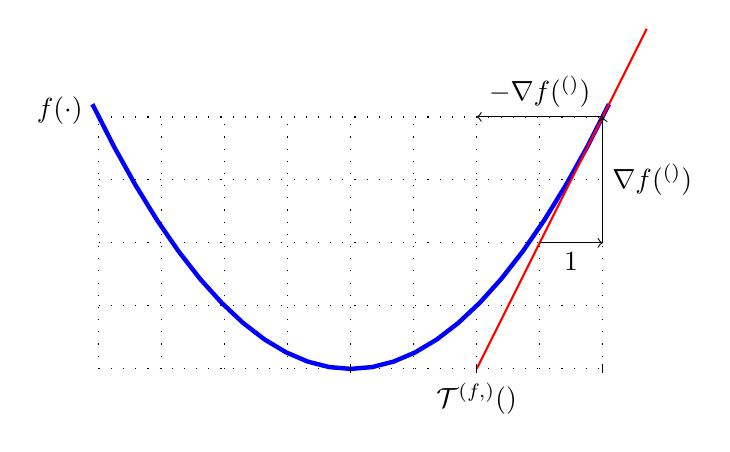
\begin{tikzpicture}[scale=0.8]
			 \draw[loosely dotted] (-4,0) grid (4,4);
			 \draw[blue, ultra thick, domain=-4.1:4.1] plot (\x,  {(1/4)*\x*\x});
			 \draw[red, thick, domain=2:4.7] plot (\x,  {2*\x - 4});
			 \draw[<-] (4,4) -- node[right] {$\nabla f(\weights^{(\itercntr)})$} (4,2);
			 \draw[->] (4,4) -- node[above] {$-\lrate \nabla f(\weights^{(\itercntr)})$} (2,4);
			 \draw[<-] (4,2) -- node[below] {$1$} (3,2) ;
			 %\draw[->] (-4.25,0) -- (4.25,0) node[right] {$a$};
			 \node[left] at (-4.1, 4.1) {$f(\cdot)$}; 
			 \draw[shift={(0,0)}] (0pt,2pt) -- (0pt,-2pt) node[below] {$\overline{\weights}$};
			 \draw[shift={(4,0)}] (0pt,2pt) -- (0pt,-2pt) node[below] {$\weights$};
			 \draw[shift={(2,0)}] (0pt,2pt) -- (0pt,-2pt) node[below] {$\mathcal{T}^{(f,\lrate)}(\weights)$};
		 \end{tikzpicture}
	 \end{center}
	 \caption{El paso básico de gradiente \eqref{equ_def_gd_basic_dict} mapea un vector $\weights$ 
	 al vector actualizado $\weights'$. Define un operador 
	 $\mathcal{T}^{(f,\lrate)}(\cdot): \mathbb{R}^{\nrfeatures} \rightarrow \mathbb{R}^{\nrfeatures}:
	  \weights \mapsto \widehat{\weights}$.}
	 \label{fig_basic_GD_step_single_dict}
 \end{figure}
 Nótese que el paso de gradiente \eqref{equ_def_gd_basic_dict} optimiza localmente - 
 en un entorno cuyo tamaño está determinado por el tamaño de paso $\lrate$ - una aproximación lineal 
 de la función $f(\cdot)$. Una generalización natural de \eqref{equ_def_gd_basic_dict} es optimizar localmente
 la función misma - en lugar de su aproximación lineal - de tal manera que:
 \begin{align} 
 \label{equ_approx_gd_step_dict}
 \widehat{\weights} = \argmin_{\weights' \in \mathbb{R}^{\dimlocalmodel}} f(\weights')\!+\!(1/\lrate)\normgeneric{\weights-\weights'}{2}^2. 
 \end{align}
 Intencionalmente usamos el mismo símbolo $\lrate$ para el parámetro en \eqref{equ_approx_gd_step_dict} 
 que en el tamaño de paso de \eqref{equ_def_gd_basic_dict}. Mientras mayor sea el valor de $\lrate$ en 
 \eqref{equ_approx_gd_step_dict}, más progreso hará la actualización en la reducción del valor de la función $f(\widehat{\weights})$. 
 Nótese que, al igual que el paso de gradiente \eqref{equ_def_gd_basic_dict}, 
 la actualización \eqref{equ_approx_gd_step_dict} también define un operador (típicamente no lineal)  
 parametrizado por la función $f(\cdot)$ y el parámetro $\lrate$. Para una función convexa  
 $f(\cdot)$, este operador es conocido como el operador proximal de $f(\cdot)$ \cite{ProximalMethods}. 
 \\
		Vea también: \gls{differentiable}, \gls{gradient}, \gls{stepsize}, \gls{neighborhood}, \gls{generalization}, \gls{convex}, \gls{proxop} },first={paso de gradiente},text={paso de gradiente}}

		\newglossaryentry{contractop}
		{name={contraction operator},
			description={An\index{contraction operator} operator $\fixedpointop: \mathbb{R}^{\nrfeatures} \rightarrow \mathbb{R}^{\nrfeatures}$
				is a contraction if, for some $\contractfac \in [0,1)$,
				\begin{equation} 
					\nonumber
					\normgeneric{ \fixedpointop \weights\!-\!\fixedpointop \weights'}{2}  \leq  \contractfac	\normgeneric{\weights\!-\!\weights'}{2} \mbox{ holds for any } \weights,\weights' \in \mathbb{R}^{\nrfeatures}.
				\end{equation}
			},
			first={contraction operator},
			text={contraction operator} 
			
			
		}
			
		\newglossaryentry{proxop}{name={operador proximal},description={Dada una funcion convexa\index{operador proximal}   
		$f(\weights')$, definimos su operador proximal como \cite{ProximalMethods,Bauschke:2017} 
	   $$\proximityop{f(\cdot)}{\weights}{\rho}\defeq \argmin_{\weights' \in \mathbb{R}^{\dimlocalmodel}} \bigg[ f(\weights')\!+\!(\rho/2) \normgeneric{\weights- \weights'}{2}^{2}\bigg] \mbox{ with } \rho > 0. $$ 
	   Como se ilustra en la Figura \ref{fig_proxoperator_opt_dict}, evaluar el operador proximal 
	   equivale a minimizar una variante penalizada de $f(\weights')$. El término de penalización es 
	   la distancia euclidiana cuadrada escalada hacia un vector dado $\weights$ (que es la entrada del operador proximal). 
	   %\Gls{convex} functions for which the proximal operator can be computed efficiently 
	   %is sometimes referred to as \emph{proximable} or \emph{simple} \cite{Condat2013}. 
	   El operador proximal puede interpretarse como una generalización del paso de gradiente, definido 
	   para una función suave y convexa $f(\weights')$. De hecho, realizar un 
	   paso de gradiente con tamaño de paso $\lrate$ en el vector actual $\weights$ 
	   es lo mismo que aplicar el operador proximal de la función $\tilde{f}(\weights')= \big( \nabla f(\weights)\big)^{T} (\weights'-\weights)$ 
	   y usar $\rho=1/\lrate$.
		   \begin{figure}[H]
		   \begin{center}
			   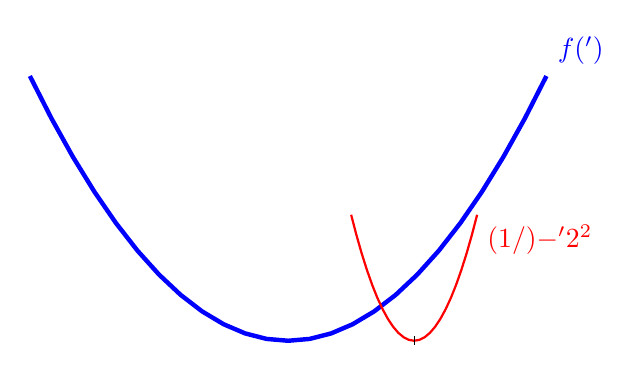
\begin{tikzpicture}[scale=0.8]
				   % Original quadratic function
				   \draw[blue, ultra thick, domain=-4.1:4.1] plot (\x, {(1/4)*\x*\x}) node[above right] {$f(\weights')$};		
				   % Quadratic function with larger curvature, centered at w = 2
				   \draw[red, thick, domain=1:3] plot (\x, {2*(\x - 2)*(\x - 2)}) node[below right] {$(1/\lrate)\normgeneric{\weights-\weights'}{2}^{2}$};
				   % Axes
				   % Minimum point of second curve
				   \draw[shift={(2,0)}] (0pt,2pt) -- (0pt,-2pt) node[below] {$\weights$};
				   %\node at (2,0.5) [anchor=north] {$\weights$};
			   \end{tikzpicture}
		   \end{center}
		   \caption{Un paso de gradiente generalizado actualiza un vector $\weights$ minimizando una versión penalizada 
			   de la función $f(\cdot)$. El término de penalización es la distancia euclidiana cuadrada escalada entre 
			   la variable de optimización $\weights'$ y el vector dado $\weights$.\label{fig_proxoperator_opt_dict}}
	   \end{figure}
	   },first={operador proximal},text={operador proximal}}

\newglossaryentry{proximable}{name={proximable},description={Una funcion \index{proximable} 
convexa para la cual el operador proximal puede calcularse de manera eficiente 
se denomina a veces proximable o simple \cite{Condat2013}.
\\
	Vea también: \gls{convex}, \gls{proxop}  },
first={proximable},text={proximable}

}


\newglossaryentry{connected}
		{name={grafo conexo},
			description={
				Un grafo no dirigido\index{grafo conexo} $\graph=\pair{\nodes}{\edges}$ es conexo si todo subconjunto no vacío $\nodes' \subset \nodes$
				tiene al menos una arista que lo conecta con $\nodes \setminus \nodes'$.
				\\
				Vea también: \gls{graph}},
			first={grafo conexo},text={grafo conexo}
		}
	
	

	

		\newglossaryentry{mvndist}
		{name={distribución normal multivariante}, 
			description={La\index{distribución normal multivariante} distribución normal multivariante, 
				denotada como $\mvnormal{\meanvecgeneric}{\covmtxgeneric}$, es un modelo de probabilidad fundamental 
				para vectores de atributos numéricos de dimensión fija $\nrfeatures$. 
				Define una familia de distribución de probabilidad sobre variables aleatorias vectoriales 
				$\featurevec \in \mathbb{R}^{\nrfeatures}$~\cite{BertsekasProb}, \cite{GrayProbBook}, \cite{Lapidoth09}. 
				Cada distribución de esta familia está completamente determinada por su vector de media 
				$\meanvecgeneric \in \mathbb{R}^{\nrfeatures}$ y su matriz de covarianza
				$\covmtxgeneric \in \mathbb{R}^{\nrfeatures \times \nrfeatures}$. Cuando la 
				matriz de covarianza $\covmtxgeneric$ es invertible, la correspondiente distribución de probabilidad se caracteriza por 
				la siguiente pdf:
				\[p(\featurevec) = 
				 \frac{1}{\sqrt{(2\pi)^{\nrfeatures} \determinant{\covmtxgeneric}}} 
				 \exp\left[ -\frac{1}{2} 
				 (\featurevec - \meanvecgeneric)^T \covmtxgeneric^{-1} 
				 (\featurevec - \meanvecgeneric) \right].
				 \]
				Nótese que esta pdf solo está definida cuando $\covmtxgeneric$ es invertible.
				   Más generalmente, cualquier variable aleatoria $\featurevec \sim \mvnormal{\meanvecgeneric}{\covmtxgeneric}$ 
				   admite la siguiente representación:
				  \[
					\featurevec = \mA \vz + \meanvecgeneric
				   \]
				   donde $\vz \sim \mvnormal{\mathbf{0}}{\mathbf{I}}$ es un vector normal estandard,  
				   y $\mA \in \mathbb{R}^{\nrfeatures \times \nrfeatures}$ satisface $\mA \mA^\top = \covmtxgeneric$. 
				   Esta representación sigue siendo válida incluso si $\covmtxgeneric$ es singular, en cuyo caso $\mA$ 
				   no es de rango completo~\cite[Ch. 23]{Lapidoth2017}.
				   La familia de distribuciones normales multivariantes es excepcional entre los modelos de probabilidad para 
				   cantidades numéricas, al menos por las siguientes razones. Primero, esta familia es cerrada bajo 
				   transformaciones afines, es decir,
				\[ 
				\featurevec \sim \mathcal{N}(\meanvecgeneric,\covmtxgeneric) \Rightarrow 
				\mB\featurevec\!+\!\vc \sim \mathcal{N}\big( \mB\meanvecgeneric+\vc,\mB \covmtxgeneric \mB^{T} \big). 
				\]
				Segundo, la distribución de probabilidad $\mathcal{N}(\mathbf{0},\covmtxgeneric)$ maximiza la 
				entropia diferencial entre todas las distribuciones con la misma matriz de covarianza $\covmtxgeneric$~\cite{coverthomas}. 
				\\ 
				Véa también: \gls{probmodel}, \gls{probdist}, \gls{stdnormvec}, \gls{diffentropy}, \gls{gaussrv}.}, 
			first={distribución normal multivariante},
			text={distribución normal multivariante}
		}
		

		\newglossaryentry{stdnormvec}
		{name={vector normal estándar}, 
			description={Un\index{vector normal estándar} vector normal estándar es un vector aleatorio 
				$\vx=\big(x_{1},\ldots,x_{\nrfeatures}\big)^{T}$ cuyas componentes son variables aleatorias gaussianas iid
				$x_{\featureidx} \sim \mathcal{N}(0,1)$. Es un caso particular de una distribución normal multivariante, 
				dado que $\vx \sim \mathcal(\mathbf{0},\mathbf{I})$.\\ 
				Véa también: \gls{iid}, \gls{gaussrv}, \gls{mvndist}, \gls{rv}.}, 
			first={vector normal estándar},
			text={vector normal estándar}
		}
		

		\newglossaryentry{statasp}{name ={aspectos estadísticos}, description={Por aspectos estadísticos\index{aspectos estadísticos} 
				de un método de aprendizaje automático, nos referimos a las propiedades de la distribución de probabilidad de su salida bajo 
				un modelo de probabilidad para los datos introducidos en el método.
				\\
				Vea también: \gls{ml}, \gls{probdist}, \gls{probmodel}, \gls{data} },first={aspectos estadísticos},text={aspectos estadísticos}}

				\newglossaryentry{compasp}{name ={aspectos computacionales}, description={Por aspectos 
				computacionales\index{aspectos computacionales} de un método de aprendizaje automático, nos referimos principalmente a los recursos 
				computacionales requeridos para su implementación.
				Por ejemplo, si un método de aprendizaje automático utiliza técnicas 
				de optimización iterativas para resolver ERM, sus aspectos computacionales incluyen: 1) cuántas 
				many operaciones aritméticas se necesitan para implementar una sola iteración(paso de gradiente); 
				y 2) cuántas iteraciones se requieren para obtener parámetros del modelo útiles. Un ejemplo 
				importante de técnica de optimización iterativa es el descenso por gradiente.
				\\
				Vea también: \gls{ml},\gls{erm}, \gls{gradstep}, \glspl{modelparam}, \gls{gd}  }, first={aspectos computacionales},text={aspectos computacionales}}
		
		\newglossaryentry{zerooneloss}{name={$\bf 0/1$ loss},
			description={La perdida $0/1$ \index{$0/1$ loss} $\lossfunczo{\pair{\featurevec}{\truelabel}}{\hypothesis}$ 
				mide la calidad de un clasificador $\hypothesis(\featurevec)$ que genera una 
				prediccion $\predictedlabel$ (por ejemplo, mediante un umbral como en \eqref{equ_def_threshold_bin_classifier_dict}) 
				para la etiqueta $\truelabel$ de un punto de datos con atributos $\featurevec$. Es igual a $0$ si 
				la prediccion es correcta, es decir, 
			$\lossfunczo{\pair{\featurevec}{\truelabel}}{\hypothesis}=0$ cuando $\predictedlabel=\truelabel$. Es igual 
			a $1$ si la prediccion es incorrecta, es decir, $\lossfunczo{\pair{\featurevec}{\truelabel}}{\hypothesis}=1$ 
			cuando $\predictedlabel\neq\truelabel$.
			\\
				Vea también: \gls{loss},\gls{classifier}, \gls{prediction},\gls{label}, \gls{datapoint},\gls{feature} },
			sort=zerooneloss, 
		   first={$0/1$ loss},text={$0/1$ loss}}
		
		\newglossaryentry{probability}{name={probabilidad},
			description={Asignamos \index{probabilidad} un valor de probabilidad, típicamente elegido en el 
				intervalo $[0,1]$, a cada evento que pueda ocurrir en un experimento aleatorio \cite{KallenbergBook,BertsekasProb,BillingsleyProbMeasure,HalmosMeasure}.},
				first={probabilidad},text={probabilidad}}


				\newglossaryentry{underfitting}{name={subajuste},
				description={Consideremos\index{subajuste} un método de aprendizaje automatico que utiliza ERM para aprender una hipótesis
				con el minimo riesgo empírico en un conjunto de entrenamiento dado.
				Dicho método presenta subajuste del conjunto de entrenamiento si no es capaz de aprender una hipótesis
				con un rieso empírico suficientemente pequeño sobre el conjunto de entrenamiento.
				Si un método sufre de subajuste, típicamente tampoco podrá aprender una hipótesis
				con un riesgo pequeño.
				\\
				Vea también: \gls{ml}, \gls{erm}, \gls{hypothesis}, \gls{minimum}, \gls{emprisk}, \gls{trainset}, \gls{risk} },
				first={subajuste},text={subajuste}
					}

\newglossaryentry{overfitting}{name={sobreajuste},description={Consideremos\index{overfitting} un 
		método de aprendizaje automático que utiliza ERM para aprender una hipótesis con el minimo riesgo empírico en 
		un conjunto de entrenamiento dado. Dicho método presenta sobreajuste del conjunto de entrenamiento si aprende 
		una hipótesis con un rieso empírico pequeño sobre el conjunto de entrenamiento pero una perdida significativamente mayor fuera de él conjunto de entrenamiento.
		\\
			Vea también: \gls{ml}, \gls{erm}, \gls{hypothesis}, \gls{minimum}, \gls{emprisk}, \gls{trainset}, \gls{loss}    },first={sobreajuste},text={sobreajuste}}

			\newglossaryentry{gdpr}{name={reglamento general de protección de datos (RGPD)},description={
				El\index{reglamento general de protección de datos (RGPD)} RGPD
				fue promulgado por la Union Europea (EU), y entró en efecto el 25 de Mayo de 2018 \cite{GDPR2016}. 
				Protege la privacidad y los derechos sobre los datos de los individuos dentro de la EU. 
				El RGPD tiene implicaciones significativas sobre cómo se recopilan, almacenan y utilizan los datos en aplicaciones de aprendizaje automático.
				Las disposiciones clave incluyen:
				\begin{itemize}
					\item Principio de minimización de datos: los sistemas de aprendizaje automático deben utilizar únicamente la cantidad necesaria de  
					datos personal para su propósito.
					\item Transparencia y explicabilidad: los sistemas de aprendizaje automático deben permitir a sus usuarios comprender 
					cómo se toman las decisiones que los afectan.
					\item Derechos del titular de los datos: los usuarios deben tener la posibilidad de acceder, rectificar y eliminar sus datos, así como oponerse a decisiones automatizadas y perfiles.
					\item Responsabilidad: las organizaciones deben garantizar una seguridad robusta de los datos y demostrar 
					cumplimiento mediante documentación y auditorías periódicas.
				\end{itemize}
				}, 
		first={reglamento general de protección de datos (RGPD)},text={RGPD}}
	
\newglossaryentry{gaussrv}{name={variable aleatoria gaussiana (VA gaussiana)},description={
		Una \index{variable aleatoria gaussiana (VA gaussiana)} variable aleatoria gaussiana estándar es una variable aleatoria
		real $x$ con función de densidad de probabilidad (pdf) \cite{papoulis,BertsekasProb,GrayProbBook}
		\begin{equation}
			\nonumber
			p(x) = \frac{1}{\sqrt{2\pi}} \exp^{-x^2/2}. 
		\end{equation}
		Dada una variable aleatoria gaussiana estándar $x$, podemos construir una variable aleatoria gaussiana general $x'$ con 
		media $\mu$ y varianza $\sigma^2$ mediante $x' \defeq \sigma (x+\mu)$. La distribución de probabilidad de una 
		variable aleatoria gaussiana se conoce como distribución normal, denotada $\mathcal{N}(\mu,\sigma)$.  \\ 
		Un vector aleatorio gaussiano $\featurevec \in \mathbb{R}^{\featuredim}$ con 
		matriz de covarianza $\mathbf{C}$ y media ${\bm \mu}$ puede construirse como 
		$\featurevec \defeq \mathbf{A} \big( \vz + {\bm \mu} \big)$. Aquí, $\mA$ 
		es cualquier matriz que satisface $\mA\mA^{T} = \mC$ y $\vz \defeq \big( z_{1},\ldots,z_{\featuredim} \big)^{T}$
		es un vector cuyos elementos son iid gaussianas estándar variables aleatorias $z_{1},\ldots,z_{\featuredim}$. Los procesos aleatorios gaussianos generalizan
		los vectores aleatorios gaussianos aplicando transformaciones lineales a 
		a secuencias infinitas de variables aleatorias gaussianas estándar \cite{Rasmussen2006Gaussian}.\\
		Las variables aleatorias gaussianas se utilizan ampliamente como modelos de probabilidad en el análisis estadístico de métodos de aprendizaje automático.
		Su importancia se debe, en parte, al teorema del límite central, que establece que el promedio de un número creciente de variables aleatorias independientes
		(aunque no sean gaussianas) converge a una variable aleatoria gaussiana \cite{ross2013first}. 
		\\
		The \gls{mvndist} is also distinct in that it represents maximum \gls{uncertainty}: 
		Among all \gls{vector}-valued \glspl{rv} with a given \gls{covmtx} $\mC$, the \gls{rv} $\vx \sim \mathcal{N}({\bm \mu}, \mathbf{C})$ 
		maximizes \gls{diffentropy} \cite[Th. 8.6.5]{coverthomas}. This makes \glspl{GaussProc} a 
		natural choice for capturing \gls{uncertainty} (or lack of knowledge) in the absence of additional 
		structural information.
		\\
		Vea también: \gls{rv}, \gls{pdf}, \gls{mean}, \gls{variance}, \gls{probdist}, \gls{covmtx}, \gls{iid}, \gls{ml} },first={variable aleatoria gaussiana (VA gaussiana)},text={VA gaussiana}
}
\newglossaryentry{clt}
{name={teorema central del límite (CLT)},
description={Consideremos una secuencia de variable aleatoria iid \( \feature^{(\sampleidx)} \), para \( \sampleidx = 1, 2, \ldots \), 
cada una con media cero y varianza finita \( \sigma^2 > 0 \). 
El \index{teorema central del límite (CLT)} teorema central del límite (CLT) establece que la suma normalizada
\[
s^{(\samplesize)} \defeq \frac{1}{\sqrt{\samplesize}} \sum_{\sampleidx = 1}^{\samplesize} \feature^{(\sampleidx)} 
\]
converge en distribución a una variable aleatoria gaussiana con media cero y varianza \( \sigma^2 \) cuando \( \samplesize \to \infty \) \cite[Proposition~2.17]{AsympVanderVaartBook}. 
Una forma elegante de derivar el CLT es mediante la funcion característica de la suma normalizada \( s^{(\samplesize)} \). 
Sea $ \phi(t) = \expect \big\{ \exp \big( j t \feature \big) \big\}$ (donde $j = \sqrt{-1}$ es la unidad imaginaria) 
la funcion característica común de cada término $\feature^{(\sampleidx)}$, y sea \( \phi^{(\samplesize)}(t) \) 
la funcion característica de \( s^{(\samplesize)} \). Definimos un operador \( \mathcal{T} \) que actúa sobre funciones de característica 
tal que
\[
\phi^{(\samplesize)}(t) = \mathcal{T}(\phi^{(\samplesize-1)})(t) \defeq \phi\left( \frac{t}{\sqrt{\samplesize}} \right) \cdot \phi^{(\samplesize-1)}\left( \frac{\sqrt{\samplesize-1}}{\sqrt{\samplesize}} t \right).
\]
Esta iteracion de punto fijo captura el efecto de añadir recursivamente una variable aleatoria iid $\featurevec^{(\samplesize)}$ 
y reescalar. Al aplicar \( \mathcal{T} \) iterativamente, se obtiene la convergencia de \( \phi^{(\samplesize)}(t) \) hacia el punto fijo
\[
\phi^*(t) = \exp\,(-t^2 \sigma^2 / 2)
\]
que es la funcion característica de una variable aleatoria gaussiana con media cero y varianza \( \sigma^2 \). 
Las generalizaciones del CLT permiten variables aleatorias dependientes o no idénticamente distribuidas \cite[Sec.~2.8]{AsympVanderVaartBook}.
\begin{figure}[H]
\centering
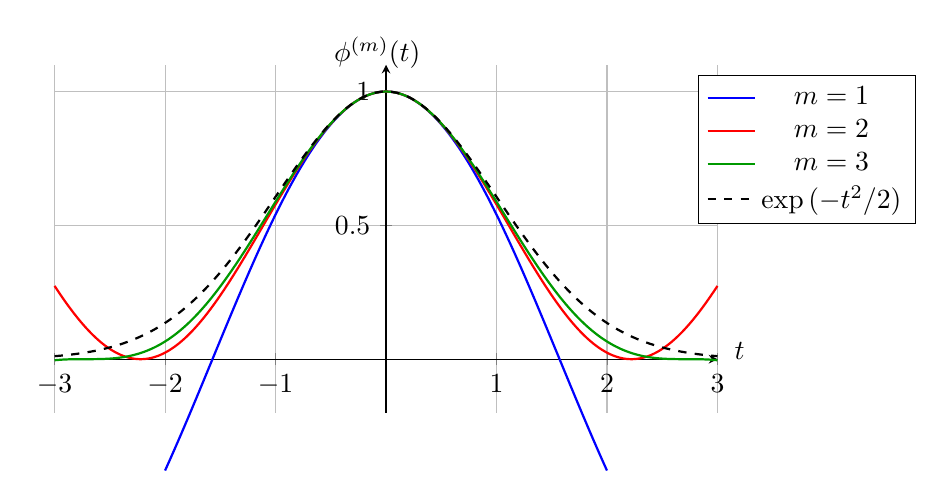
\begin{tikzpicture}
\begin{axis}[
width=10cm,
height=6cm,
xlabel={},
ylabel={},
legend style={at={(0.97,0.97)}, anchor=north west},
domain=-3:3,
ylabel style={
yshift=10pt   % shift label up by 10pt
},
samples=400,
ymin=-0.2, ymax=1.1,
axis lines=middle,
clip=false,
grid=both,
]
\addplot[thick, blue,domain=-2:2] {cos(x/sqrt(1) r)^1};
\addlegendentry{$m=1$}
\addplot[thick, red] {cos(x/sqrt(2) r)^2};
\addlegendentry{$m=2$}
\addplot[thick, green!60!black] {cos(x/sqrt(3) r)^3};
\addlegendentry{$m=3$}
\addplot[thick, dashed, black] {exp(-x^2/2)};
\addlegendentry{$\exp\,(-t^2/2)$}
\node[anchor=south, rotate=0] at (axis cs:-0.08,1.05) {$\phi^{(m)}(t)$};
\node[anchor=north, rotate=0] at (axis cs: 3.2,0.1) {$t$};
\end{axis}
\end{tikzpicture}
\caption{Funciones característica de sumas normalizadas de variables aleatorias iid $x^{(\sampleidx)} \in \{-1,1\}$ 
para $\sampleidx=1,\ldots,\samplesize$, comparadas con el límite gaussiano.}
\end{figure}
Vea tambien: \gls{rv}, \gls{gaussrv}.},
first={teorema central del límite (CLT)},
text={CLT}
}



\newglossaryentry{GaussProc}
{name={proceso gaussiano (GP)},
  description={Un \index{proceso gaussiano (GP)}GP es una colección de variables aleatorias
  	$\{f(\featurevec)\}_{\featurevec \in \featurespace}$ indexadas por valores de entrada $\featurevec$ 
  	de un cierto espacio de entrada $\featurespace$, tal que, para cualquier subconjunto finito 
  	$\featurevec^{(1)}, \ldots, \featurevec^{(\samplesize)} \in \featurespace$, 
  	las variables aleatorias correspondientes $f(\featurevec^{(1)}), \ldots, f(\featurevec^{(\samplesize)})$ 
  	tienen una distribución conjunta gaussiana multivariante:
  	\[
  	\left( f(\featurevec^{(1)}), \ldots, f(\featurevec^{(\samplesize)}) \right) \sim \mathcal{N}(\boldsymbol{\mu}, \mathbf{K}).
  	\]
  	Para un espacio de entrada $\featurespace$ fijo, un GP queda completamente especificado (o parametrizado) por:
  	\begin{itemize}
  		\item una función media $\mu(\featurevec) = \expect\{ f(\featurevec)\}$
  		\item y una función de covarianza $\kernelmap{\featurevec}{\featurevec'} = \expect\{ \big(f(\featurevec)-\mu(\featurevec)\big) \big(f(\featurevec')-\mu(\featurevec')\big) \big\}$.
  	\end{itemize}
  	\text{Ejemplo:} Podemos interpretar la distribución de temperatura en Finlandia (en un instante específico)
  	como la realización de un GP $f(\featurevec)$, donde cada entrada 
  	$\featurevec = (\text{lat}, \text{lon})$ representa una ubicación geográfica. 
  	Las observaciones de temperatura de las estaciones meteorológicas de FMI constituyen 
  	muestras de $f(\featurevec)$ en ubicaciones específicas (vea la Figura \ref{fig_gp_FMI_dict}). 
  	Un GP nos permite predecir la temperatura en las cercanías de las estaciones meteorológicas 
  	y cuantificar la incertidumbre de dichas predicciones.
  	\begin{figure}[H]
  	\begin{center}
  \begin{tikzpicture}
\begin{axis}[
	axis equal,
	hide axis,
	scale=1.2,
	xmin=17, xmax=32,
	ymin=55, ymax=71,
	clip=true
	]
	% --- Finland border (polyline) ---
	\addplot[
	color=black,
	thick
	] table [x=lon, y=lat, col sep=comma] {../../assets/finland_border.csv};
	% --- FMI sample stations ---
	\addplot[
	only marks,
	mark=*,
	mark options={fill=blue},
	color=black
	] table [x=lon, y=lat, col sep=comma] {../../assets/fmi_stations_subset.csv};
	% Draw manual axes
	\draw[->, thick] (axis cs:19,59) -- (axis cs:25.5,59) node[anchor=west] {lon};
	\draw[->, thick] (axis cs:19,59) -- (axis cs:19,65.5) node[anchor=south] {lat};
\end{axis}
\end{tikzpicture}
\vspace*{8mm}
\end{center}
\caption{Podemos interpretar la distribución de temperatura sobre Finlandia como una realización 
	de un GP indexado por coordenadas geográficas y muestreado en estaciones meteorológicas de FMI
	(indicadas por puntos azules). \label{fig_gp_FMI_dict}}
\end{figure}
Véa también: \gls{rv}, \gls{mean}, \gls{function}, \gls{realization}, \gls{fmi}, \gls{sample}, \gls{uncertainty}.}, 
first = {GP}, 
	text = {GP}
}



\newglossaryentry{trustAI}{name={inteligencia artificial confiable (IA confiable)},description=
		{Además de los aspectos computacionales y los aspectos estadísticos, un tercer aspecto principal 
		en el diseño de métodos de aprendizaje automático es su confiabilidad\index{inteligencia artificial confiable (IA confiable)} \cite{pfau2024engineeringtrustworthyaideveloper}. 
		La Unión Europea ha propuesto siete requisitos clave (KRs) para una inteligencia artificial confiable 
		(que típicamente se basa en métodos de aprendizaje automático) \cite{ALTAIEU}: 
	\begin{enumerate}[label=\arabic*)]
		\item KR1 - Agencia y supervisión humana;
		\item KR2 - Robustez técnica y seguridad;
		\item KR3 - Privacidad y gobernanza de los datos;
		\item KR4 - Transparencia;
		\item KR5 - Diversidad, no discriminación y equidad; 
		\item KR6 - Bienestar social y ambiental;
		\item KR7 - Responsabilidad. 
	\end{enumerate}
	.\\
		Vea también: \gls{compasp}, \gls{statasp}, \gls{ml}, \gls{ai} },first={inteligencia artificial confiable (IA confiable)},text={trustworthy AI}}

\newglossaryentry{sqerrloss}{name={pérdida de error cuadrático},description={La perdida de
	error cuadrático\index{pérdida de error cuadrático} mide el error de predicción de una 
	hipótesis $\hypothesis$ al predecir una etiqueta numérica $\truelabel \in \mathbb{R}$ 
	a partir de los atributos $\featurevec$ de un punto de datos. Se define 
como 
\begin{equation} 
\nonumber
%	\label{equ_squared_loss_gls}
\lossfunc{(\featurevec,\truelabel)}{\hypothesis} \defeq \big(\truelabel - \underbrace{\hypothesis(\featurevec)}_{=\predictedlabel} \big)^{2}. 
\end{equation} 
.\\
		Vea también: \gls{loss}, \gls{prediction}, \gls{hypothesis}, \gls{label}, \gls{feature}, \gls{datapoint} },first={pérdida de error cuadrático},text={pérdida de error cuadrático}}


\newglossaryentry{projection}{name={proyección}, 
  description={Consideremos\index{proyección} un subconjunto $\paramspace \subseteq \mathbb{R}^{\dimlocalmodel}$ del 
   espacio euclidiano de dimensión $\dimlocalmodel$. Definimos la proyección $\projection{\paramspace}{\weights}$
   de un vector $\weights \in \mathbb{R}^{\dimlocalmodel}$ sobre $\paramspace$ como
	\begin{equation} 
	  \label{equ_def_proj_generic_dict}
	  \projection{\paramspace}{\weights} = \argmin_{\weights' \in \paramspace} \normgeneric{\weights - \weights'}{2}. 
	\end{equation}
	 En otras palabras, $\projection{\paramspace}{\weights}$ es el vector en $\paramspace$ más cercano a $\weights$. 
	 La proyección está bien definida solo para aquellos subconjuntos $\paramspace$ para los cuales existe el minimo anterior \cite{BoydConvexBook}.
	 \\
		Vea también: \gls{minimum}},
	 first={proyección},text={proyección}}


	 \newglossaryentry{projgd}{name={descenso por gradiente proyectado (GD proyectado)},
	 description={Consideremos un método basado en ERM que utiliza un modelo parametrizado con  
	 un espacio de parámetros $\paramspace \subseteq \mathbb{R}^{\dimlocalmodel}$. Aun si la
	 funcion objetivo de ERM es suave, no podemos usar el descenso por gradiente básico, ya 
	 ya que este no toma en cuenta las restricciones sobre la variable de optimización (es decir, los parámetros del modelo). 
	 El descenso por gradiente proyectado\index{descenso por gradiente proyectado (GD proyectado)} 
	 extiende el descenso por gradiente básico para controlar restricciones sobre la variable de optimización(es decir, los parámetros del modelo). 
	 Una sola iteración del descenso por gradiente proyectado consiste primero en realizar un paso de gradiente
	 y luego proyectar el resultado sobre el espacio de parámetros
	 \begin{figure}[H]
		 \begin{center}
			 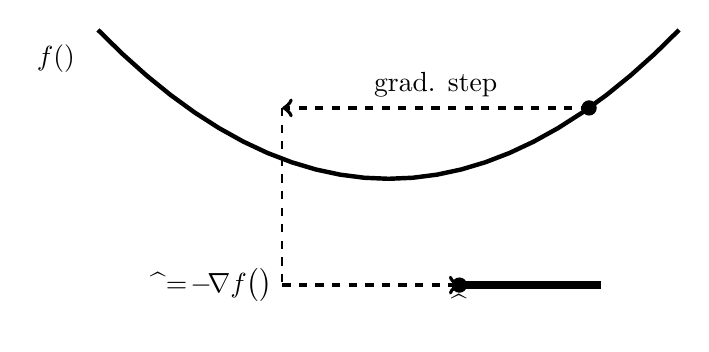
\begin{tikzpicture}[scale=0.9]
				 \node [right] at (-5.1,1.7) {$f(\weights)$} ;
				 \draw[ultra thick, domain=-4.1:4.1] plot (\x,  {(1/8)*\x*\x});
			 %	\draw[dashed, thick, domain=1:3.6] plot (\x,  {\x - 1}) node[right] {$ f\big(\weights^{(\itercntr)}\big)\!+\!\big(\weights\!-\!\weights^{(\itercntr)}\big)^{T} \nabla f\big(\weights^{(\itercntr)}\big)$};
				 \draw [fill] (2.83,1) circle [radius=0.1] node[right] {$\weights$};
				 \draw[line width =0.5mm,dashed,->] (2.83,1) -- node[midway,above] {grad. step} (-1.5,1);
				 \draw[line width =0.2mm,dashed] (-1.5,1) --(-1.5,-1.5)  node [below, left]{$\widehat{\weights}=\weights\!-\!\lrate \nabla f\big(\weights\big)$} ;
				 \draw[line width =0.5mm,dashed,->] (-1.5,-1.5)  -- node[midway,above] {} (1,-1.5) ; 
				 \draw [fill] (1,-1.5) circle [radius=0.1] node[below] {$\projection{\paramspace}{\widehat{\weights}}$};
				 \draw[line width=1mm] (1,-1.5) -- (3,-1.5) node[midway, above] {$\paramspace$};
			 \end{tikzpicture}
			 \vspace*{-5mm}
		 \end{center}
		 \caption{\gls{gd} proyectado amplía un \gls{gradstep} básico con una \gls{projection} de regreso 
		 al conjunto de restricciones $\paramspace$.}
		 \label{fig_projected_GD_dict}
	 \end{figure}
	 .\\
		Vea también:\gls{erm}, \gls{model}, \gls{paramspace}, \gls{objfunc}, \gls{smooth}, \gls{gd}, \glspl{modelparam}, \gls{gradstep}  },first={descenso por gradiente proyectado (GD proyectado)},text={GD proyectado}}
	 
		

	 \newglossaryentry{diffpriv}
	 {name=privacidad diferencial (DP),
	  description={
		  Consideremos\index{differential privacy (DP)} un método de aprendizaje automático $\algomap$ que recibe como entrada un conjunto de datos (por ejemplo, el conjunto de entrenamiento
		  usado para ERM) y entrega una salida $\algomap(\dataset)$. La salida 
		  puede ser los parámetros del modelo aprendidos o las predicciones para ciertos puntos de datos. 
		  DP es una medida precisa de la filtración de privacidad ocasionada al revelar dicha salida.
		 Aproximadamente, un método de aprendizaje automático es diferencialmente privado si la distribución de probabilidad
		  de la salida $\algomap(\dataset)$ no cambia significativamente cuando se modifica el atributo sensible
		  de un solo punto de datos del conjunto de entrenamiento. Nótese que la DP 
		  se basa en un modelo de probabilidad para un método de aprendizaje automático, es decir, interpretamos su salida $\algomap(\dataset)$ 
		  como la realización de una variable aleatoria. La aleatoriedad en la salida puede asegurarse añadiendo intencionalmente la
		  realización de una variable aleatoria auxiliar (ruido) a la salida del método de aprendizaje automático.
		  \\
		  Vea también: \gls{ml}, \gls{dataset}, \gls{trainset}, \gls{erm}, \glspl{modelparam}, \gls{prediction}, \gls{datapoint}, \gls{privleakage}, \gls{probdist}, \gls{sensattr}, \gls{probmodel}, \gls{realization}, \gls{rv}  }, 
		 first = {privacidad diferencial (DP)}, text={DP} 
	 }

	 \newglossaryentry{robustness}
	 {name={robustez},
		 description={La robustez\index{robustez} es un requisito clave para la IA confiable. 
		 Se refiere a la propiedad de un sistema de aprendizaje automático de mantener un rendimiento aceptable incluso 
		 cuando se somete a diferentes formas de perturbaciones. Estas perturbaciones pueden afectar los
		 atributos de un punto de datos con el fin de manipular la prediccion producida 
		 por un modelo de aprendizaje automático ya entrenado. La robustez también abarca la estabilidad
		 de los métodos basados en ERM frente a perturbaciones en el conjunto de entrenamiento. 
		 Estas perturbaciones pueden ocurrir como parte de ataque de envenenamiento de datos.\\ 
		 Véa también: \gls{trustAI}, \gls{ml}, \gls{feature}, \gls{datapoint}, \gls{prediction}, 
		 \gls{model}, \gls{stability}, \gls{erm}, \gls{trainset}, \gls{datapoisoning}, \gls{attack}.
		 }, 
		 first={robustez}, 
		 text={robustez} 
	 }
	 
	 
\newglossaryentry{stability}
{name={estabilidad},
	description={
		La estabilidad\index{estabilidad} es una propiedad deseable de un método de aprendizaje automático $\algomap$ que mapea un 
		conjunto de datos$\dataset$ (por ejemplo, un conjunto de entrenamiento) a una salida $\algomap(\dataset)$, como 
		parametros del modelo aprendidos o la predicción para un punto de datos específico. De forma intuitiva, 
		$\algomap$ es estable si pequeños cambios en el conjunto de datos de entrada $\dataset$ provocan pequeños 
		cambios en la salida $\algomap(\dataset)$. Existen varias nociones formales de estabilidad que permiten 
		establecer cotas sobre el error de generalización o el riesgo del método; véase \cite[Cap.~13]{ShalevMLBook}.
		Para desarrollar la intuición, considérese los tres conjuntos de datos representados en la 
		Fig.~\ref{fig_three_data_stability}, cada uno de los cuales es igualmente probable bajo los mismos datos
		generada por una distribucion de probabilidad. Dado que los parametros del modelo óptimos están determinados por esta 
		distribución de probabilidad subyacente, un método preciso de aprendizaje automático $\algomap$ debería devolver la misma (o muy similar) 
		salida $\algomap(\dataset)$ para los tres conjuntos de datos. En otras palabras, cualquier $\algomap$ útil debe ser 
		robusto frente a la variabilidad en las realizaciónes de muestras provenientes de la misma distribución de probabilidad, 
		es decir, debe ser estable. 
		\begin{figure}[H]
			\centering
			\begin{tikzpicture}
				\begin{axis}[
				%title={Stem Plots of 3 Datasets},
				    axis lines=none,
					xlabel={$\sampleidx$},
					ylabel={},
					legend pos=north west,
					ymin=0, ymax=10,
					xtick={1,2,3,4,5},
				%	ymajorgrids=true,
					grid style=dashed,
					every axis plot/.append style={very thick}
					]
					% Dataset 1
					\addplot+[only marks,mark=*] coordinates {
						(1,2) (2,4) (3,3) (4,5) (5,7)
					};
				%	\addlegendentry{$\dataset^{(*)}$}
					% Dataset 2
					\addplot+[only marks,mark=square*] coordinates {
						(1,3) (2,2) (3,6) (4,4) (5,5)
					};
				%	\addlegendentry{$\dataset^{(\square)}$}
					% Dataset 3
					\addplot+[only marks,mark=triangle*] coordinates {
						(1,5) (2,7) (3,4) (4,6) (5,3)
					};
				%	\addlegendentry{$\dataset^{(\triangle)}$}
				\end{axis}
			\end{tikzpicture}
			\caption{Tres conjuntos de datos diferentes $\dataset^{(*)}$, $\dataset^{(\square)}$, y $\dataset^{(\triangle)}$, 
				cada uno muestreado independientemente del mismo distribución de datos generador de datos. Un método estable de aprendizaje automático 
				debería generar resultados similares al entrenarse con cualquiera de estos conjuntos de entrenamiento. \label{fig_three_data_stability}}
		\end{figure}.
		\\
		Vea también: \gls{ml}, \gls{dataset}, \gls{trainset}, \glspl{modelparam}, \gls{prediction}, \gls{datapoint}, \gls{generalization}, \gls{risk}, \gls{data}, \gls{probdist},   }, 
	first = {stability}, text={stability} 
}

\newglossaryentry{privprot}
{name=protección de la privacidad,
    description={Consideremos\index{protección de la privacidad} un método de aprendizaje automático $\algomap$ que recibe como entrada 
	 un conjunto de datos $\dataset$ y entega una salida $\algomap(\dataset)$. La salida 
	 puede ser los parametros del modelo aprendidos $\widehat{\weights}$ o una predicción
	 $\learnthypothesis(\featurevec)$ obtenida para un punto de datos específico con atributos
	 $\featurevec$. Muchas aplicaciones importantes de aprendizaje automático involucran puntos de datos 
		que representan a personas. Cada punto de datos se caracteriza por atributos $\featurevec$, 
		posiblemente una etiqueta $\truelabel$, y un atributo sensible $\sensattr$ (por ejemplo, un diagnóstico medico). 
		Mas o menos, la protección de la privacidad significa que debería ser imposible inferir, de la salida $\algomap(\dataset)$, 
		cualquier atributo sensible de los puntos de datos en $\dataset$. Matemáticamente, la protección de privacidad requiere que  
		el mapeo $\algomap(\dataset)$ no sea invertible. En general, el solo hacer que  $\algomap(\dataset)$ no sea invertible 
		no es suficiente. Necesitamos que sea suficientemente no invertible. 
		\\
		Vea también:  \gls{ml}, \gls{dataset}, \glspl{modelparam}, \gls{prediction}, \gls{datapoint}, \gls{feature}, \gls{label}, \gls{sensattr} }, 
	first = {protección de la privacidad}, text={protección de la privacidad} 
}

\newglossaryentry{privleakage}
{
	name=filtración de privacidad,
	description={Consideremos\index{privacy leakage} una aplicacion de aprendizaje automático que procesa un
	conjunto de datos $\dataset$ y produce una salida, como las predicciones
	obtenidas para nuevos puntos de datos. Se produce una filtración de privacidad 
	cuando la salida contiene información privada sobre un atributo de un 
	punto de datos (que podría representar a una persona) en $\dataset$. Basado en el modelo de probabilidad
	para la generacion de los datos, podemos medir la filtración de privacidad usando la información mutua (MI)
	entre la salida y el atributo sensible. Otra medida cuantitativa de la filtración de privacidad 
	es la privacidad diferencial (DP). Las relaciones entre las diferentes medidas de filtración de privacidad han sido estudiadas en la literatura (véa \cite{InfThDiffPriv}). 
	\\
		Vea también: \gls{ml}, \gls{dataset}, \gls{prediction}, \gls{datapoint},  \gls{feature}, \gls{probmodel}, \gls{data}, \gls{mutualinformation}, \gls{diffpriv} }, 
	first = {filtración de privacidad}, text={filtración de privacidad} 
}



\newglossaryentry{probmodel}
{
	name=modelo probabilístico,
	description={Un modelo probabilístico\index{modelo probabilístico} interpreta los puntos de datos
		como realizaciónes de variables aleatorias con una distribución de probabilidad conjunta. Esta distribución de probabilidad conjunta típicamente 
		incluye parametros que deben seleccionarse manualmente or o aprenderse usando métodos de inferencia estadística  
		como la estimación por máxima verosimilitud \cite{LC}.
		\\
		Vea también: \gls{model}, \gls{datapoint}, \gls{realization}, \gls{rv}, \gls{probdist}, \gls{parameters}, \gls{maxlikelihood} }, 
	first = {modelo probabilístico}, text={modelo probabilístico} 
}



\newglossaryentry{mean}
		{name={media},
			plural={medias},
			description={La\index{media} media de una variable aleatoria $\featurevec$, que toma
				valores en un espacio euclidiano $\mathbb{R}^{\dimlocalmodel}$, es su
				esperanza $\expect\{\featurevec\}$. Se define como la integral de Lebesgue
				de $\featurevec$ con respecto a la distribución de probabilidad subyacente $P$ (por ejemplo,
				ver \cite{RudinBookPrinciplesMatheAnalysis} o \cite{BillingsleyProbMeasure}), es decir,
				\[
					\expect\{\featurevec\} = \int_{\mathbb{R}^{\dimlocalmodel}} \vx \, \mathrm{d}P(\vx).
				\]
				Es útil pensar en la media como la solución del siguiente problema de minimización de \gls{risk}
				\cite{BertsekasProb}:
				\[
					\expect\{\featurevec\} = \aargmin_{\vc \in \mathbb{R}^{\nrfeatures}}
					\expect \big\{\normgeneric{\featurevec - \vc}{2}^{2}\big \}.
				\]
				También usamos el término para referirnos al promedio de una secuencia finita
				$\vx^{(1)}, \ldots, \vx^{(\samplesize)} \in \mathbb{R}^{\dimlocalmodel}$. Sin embargo,
				estas dos definiciones son esencialmente las mismas. De hecho, podemos usar la secuencia
				$\vx^{(1)}, \ldots, \vx^{(\samplesize)} \in \mathbb{R}^{\dimlocalmodel}$ para construir una
				variable aleatoria discreta $\widetilde{\vx}=\vx^{(I)}$, con el índice $I$ elegido uniformemente
				al azar del conjunto $\{1, \ldots, \samplesize\}$. La media de $\widetilde{\vx}$ es
				precisamente el promedio $({1}/{\samplesize}) \sum_{\sampleidx=1}^{\samplesize} \vx^{(\sampleidx)}$.
				\\
				Véa también: \gls{rv}, \gls{expectation}, \gls{probdist}.},
			first={media},
			text={media}
		}

\newglossaryentry{median}
{name={mediana}, 
 description={Una\index{mediana} mediana $\med(x)$ de una variable aleatoria real $x$ 
 es cualquier número $m \in \mathbb{R}$ tal que $\prob{ x \leq m} \geq 1/2$ y $\prob{ x \geq m} \geq 1/2$ \cite{LC}.
 \begin{figure}[H]
	\begin{center}
	\begin{tikzpicture}
  \begin{axis}[
    axis lines=middle,
    xlabel={$m$},
    ylabel={},
    ymin=0, ymax=1.1,
    xmin=-2, xmax=6,
    xtick=\empty,
    ytick={0,1/2,1},
    domain=-2:6,
    samples=200,
    width=10cm,
    height=6cm,
    smooth,
    enlargelimits=true,
    clip=false
  ]
    \addplot[thick, blue, name path=cdf] {1/(1 + exp(-(x - 1)))} node[pos=0.5, above, yshift=15pt] {$\prob{x \leq m}$};
    \draw[dashed, gray] (axis cs:1,0) -- (axis cs:1,0.5);
    \draw[dashed, gray] (axis cs:-2,0.5) -- (axis cs:1,0.5);
    \filldraw[red] (axis cs:1,0.5) circle (2pt);
  \end{axis}
\end{tikzpicture} 
\end{center}
 \end{figure}  
 Podemos definir la mediana $\med(\dataset)$ de un conjunto de datos
 $\dataset = \{ x^{(1)}, \ldots, x^{(\samplesize)} \in \mathbb{R} \}$ 
 mediante una variable aleatoria específica $\tilde{x}$ asociada naturalmente con $\dataset$. 
 En particular, esta variable aleatoria se construye como $\tilde{x} = x^{(I)}$, donde el índice $I$ 
 se elige uniformemente al azar del conjunto $\{1,\ldots,\samplesize\}$, es decir, 
 $\prob{I = \sampleidx} = 1/\samplesize$ para todo $\sampleidx = 1,\ldots,\samplesize$. 
 Si la variable aleatoria $x$ es integrable, una mediana de $x$ es la solución del siguiente problema de optimización: 
 $$\min_{x' \in \mathbb{R}} \expect{|x - x'|}.$$ 
 Al igual que la media, la mediana de un conjunto de datos $\dataset$ también puede usarse 
 para estimar los parametros del modelo de un modelo de probabilidad subyacente. Comparada con la media, 
 la mediana es más robusta frente a un valor atípico. Por ejemplo, la mediana de un conjunto de datos $\dataset$ 
 con más de un punto de datos no cambia aunque aumentemos arbitrariamente el valor del mayor elemento de $\dataset$. 
 En contraste, la media sí lo haría.
 \definecolor{darkgreen}{rgb}{0.0, 0.5, 0.0}
  	\begin{figure}[H]
		\centering
		\begin{tikzpicture}[scale=0.7, y=0.5cm, x=0.5cm]
			\begin{scope}
				\foreach \x/\y in {
					1/2, 4/3, 7/4
				} {
					\draw[dashed, gray] (\x, 0) -- (\x, \y);
					\filldraw[blue] (\x, \y) circle (2pt);
					\node[circle, inner sep=0pt] (ptA\x) at (\x, \y) {};
				}
				\draw[dashed, thick, darkgreen] (0.5, 3) -- (10.5, 3) node[right] {$\med(\dataset)$};
				\node at (5.5, -4) {(a) conjunto de datos original $\dataset$.};
			\end{scope}
			\begin{scope}[xshift=12cm]
				\foreach \x/\y in {
					1/2, 4/3, 7/10
				} {
					\draw[dashed, gray] (\x, 0) -- (\x, \y);
					\filldraw[blue] (\x, \y) circle (2pt);
					\node[circle, inner sep=0pt] (ptB\x) at (\x, \y) {};
				}
				\draw[dashed, thick, darkgreen] (0.5, 3) -- (10.5, 3) node[right] {$\med\big(\widetilde{\dataset}\big)$};
				\node[above right=2pt and 2pt, red] at (ptB7) {outlier};
				\node at (5.5, -4) {(b) conjunto de datos ruidoso $\widetilde{\dataset}$ con un valor atípico.};
			\end{scope}
		\end{tikzpicture}
		\caption{La mediana es robusta frente a la presencia de punto atípico.}
	\end{figure}
	Véa también: \gls{mean}, \gls{robustness}, \gls{outlier}.}, 
	first = {mediana}, 
	text={mediana} 
}


\newglossaryentry{variance}
{
	name={varianza},
	description={La\index{varianza} varianza de una variable aleatoria real $\feature$ se define como la esperanza
		$\expect\big\{ \big( x - \expect\{x \} \big)^{2} \big\}$ de la diferencia cuadrada entre $\feature$ 
		y su esperanza $\expect\{x \}$. Extendemos esta definición a variables aleatorias vectoriales$\featurevec$ 
		como $\expect\big\{ \big\| \featurevec - \expect\{\featurevec \} \big\|_{2}^{2} \big\}$.
		\\
		Vea también: \gls{rv}, \gls{expectation} } ,
		first={varianza},text={varianza} 
}

\newglossaryentry{nn}
{
	name={vecino más cercano (NN)},
	description={Los métodos de vecino más cerano (NN)\index{vecino más cercano (NN)} aprenden una hipótesis
		$\hypothesis: \featurespace \rightarrow \labelspace$ cuyo valor $\hypothesis(\featurevec)$ 
		se determina únicamente por los vecinos más cercanos dentro de un conjunto de datos. Distintos 
		métodos usan diferentes medidas para determinar los vecinos más cercanos. Si los puntos de datos
		se caracterizan por vector de atributos numéricos, podemos usar la distancia euclidiana como medida.  
		the metric.
		\\
		Vea también: \gls{hypothesis}, \gls{neighbors}, \gls{dataset}, \gls{datapoint}, \gls{featurevec} },
	first={vecino más cercano (NN)},text={NN} 
}

\newglossaryentry{neighborhood}
{
	name={entorno},
	description={El\index{entorno} entorno de un nodo $\nodeidx \in \nodes$ es 
	el subconjunto de nodos constituido por los vecinos de $\nodeidx$.
	\\
		Vea también: \gls{neighbors}},
	first={entorno},text={entorno} 
}

\newglossaryentry{neighbors}
{
	name={vecinos},
	description={Los\index{vecinos} vecinos de un nodo $\nodeidx \in \nodes$ 
	dentro de una red de aprendizaje federado (red FL) son los nodos $\nodeidx' \in \nodes \setminus \{ \nodeidx\}$ conectados con $\nodeidx$ por una arista.
	\\
	Vea también: \gls{empgraph} },
	first={vecinos},text={vecinos} 
}

\newglossaryentry{bias}
{
	name={sesgo},
	description={Consideremos\index{sesgo} un método de aprendizaje automático que utiliza un espacio de hipótesis $\hypospace$ parametrizado. 
		Este aprende los parametros del modelo $\weights \in \mathbb{R}^{\dimlocalmodel}$ utilizando el conjunto de datos $$ \dataset=\big\{ \pair{\featurevec^{(\sampleidx)}}{\truelabel^{(\sampleidx)}} \big\}_{\sampleidx=1}^{\samplesize}.$$ 
		Para analizar las propiedades del método de aprendizaje automático, típicamente interpretamos los puntos de datos como realizaciónes
		de iid. variables aleatorias, $$ \truelabel^{(\sampleidx)} = \hypothesis^{(\overline{\weights})}\big( \featurevec^{(\sampleidx)} \big) + \bm{\varepsilon}^{(\sampleidx)}, \sampleidx=1,\ldots,\samplesize.$$ 
		Entonces podemos interpetar el método de aprendizaje automático como un estimador $\widehat{\weights}$ 
		calculado a partir de $\dataset$ (por ejemplo, resolviendo ERM). El sesgo (cuadrado) del estimador $\widehat{\weights}$ 
		se define como $\biasterm^{2} \defeq \big\| \expect \{ \widehat{\weights}  \}- \overline{\weights}\big\|_{2}^{2}$. 
		\\
		Vea también: \gls{ml}, \gls{hypospace}, \glspl{modelparam}, \gls{datapoint}, \gls{realization}, \gls{iid}, \gls{rv}, \gls{erm}},
		first={sesgo},text={sesgo} 
}

\newglossaryentry{classification}
{name={clasificación},
description={La clasificación\index{classification} es la tarea de determinar una
	etiqueta $\truelabel$  con valor discreto para un punto de datos, basado únicamente en sus 
	atributos $\featurevec$. La etiqueta $\truelabel$ pertenece a un conjunto finito, como por ejemplo 
	$\truelabel \in \{-1,1\}$ o $\truelabel \in \{1,\ldots,19\}$, y representa la 
	categoría a la que pertenece el punto de datos.
	\\
		Vea también: \gls{datapoint}, \gls{feature} },
	first={clasificación},text={clasificación} 
}


\newglossaryentry{privfunnel}
{name={embudo de privacidad},
description={El\index{privacy funnel} embudo de privacidad es un método para aprender atributos 
	amigables con la privacidad de los puntos de datos \cite{PrivacyFunnel}.
	\\
		Vea también: \gls{feature}, \gls{datapoint} },
first={embudo de privacidad},text={embudo de privacidad} 
}




\newglossaryentry{condnr}
{
	name={número de condición},
	description={El número de condición\index{número de condición} $\kappa(\mathbf{Q}) \geq 1$ de una 
		matriz definida positiva $\mathbf{Q} \in \mathbb{R}^{\featurelen \times \featurelen}$ es el cociente 
		$\alpha /\beta  $ entre el 
		mayor $\alpha$ y el menor $\beta$ de 
		$\mathbf{Q}$. El número de condición es útil para el análisis de métodos de aprendizaje automático. 
		La complejidad computacional de los métodos de gradiente para regresión lineal depende críticamente del número 
		de condición de la matriz $\mQ = \mX \mX^{T}$, donde $\mX$  es la matriz de atributos 
		del conjunto de entrenamiento. Es por eso que desde una perspectiva computacional, preferimos atributos de los 
		puntos de datos que hagan que $\mQ$ tenga un número de condición cercano a $1$.
		\\
		Vea también: \gls{ml}, \gls{gdmethods}, \gls{linreg}, \gls{featuremtx}, \gls{trainset}, \gls{feature}, \gls{datapoint}},first={número de condición},text={número de condición} 
}

\newglossaryentry{classifier}
{
	name={clasificador},
	description={Un clasificador\index{clasificador} es una hipótesis (función) $\hypothesis(\featurevec)$ 
		usada para predecir una etiqueta que toma valores de un espacio de etiquetas finito. Podemos usar directamente 
		el valor $\hypothesis(\featurevec)$ como predicción $\predictedlabel$ para 
		la etiqueta. Pero normalmente se usa una función $\hypothesis(\cdot)$ que entrega 
		una cantidad numérica. La predicción es obtenida a travez de un paso de umbral. 
		Por ejemplo, en un problema de clasificación binaria con \label{labelspace} $\labelspace \in  \{ -1,1\}$, 
		podríamos usar una hipótesis de valores reales $\hypothesis(\featurevec) \in \mathbb{R}$ 
		como clasificador. Una predicción $\predictedlabel$ puede obtenerse mediante:  
		 \begin{equation} 
		 	\label{equ_def_threshold_bin_classifier_dict}
		 	\predictedlabel =1   \mbox{ for } \hypothesis(\featurevec)\!\geq\!0 \mbox{ and } 	\predictedlabel =-1  \mbox{ otherwise.}
	 		\end{equation}
		Podemos caracterizar un clasificador mediante sus regiónes de decisión $\decreg{a}$, para 
		cada valor posible de etiqueta $a \in \labelspace$.
		\\
		Vea también: \gls{hypothesis}, \gls{label}, \gls{labelspace}, \gls{prediction}, \gls{classification}, \gls{decisionregion}  },first={clasificador},text={clasificador} 
}

\newglossaryentry{emprisk}
{name={riesgo empírico},
 description={El rieso empírico empírico\index{riesgo empírico} $\emprisk{\hypothesis}{\dataset}$ 
 	de una hipótesis sobre un conjunto de datos $\dataset$ es la perdida promedio incurrida 
 	por $\hypothesis$ al aplicarse a los puntos de datos en el $\dataset$.
	 \\
	 Vea también: \gls{risk}, \gls{hypothesis}, \gls{dataset}, \gls{loss}, \gls{datapoint} },
 first={riesgo empírico},text={riesgo empírico} 
}

% is it not the number of edges connected to the node instead of the neigbors?  could be the same thing, just wondering about the actual definition here. 
\newglossaryentry{nodedegree}
{name={grado de nodo},
	description={El grado\index{grado de nodo} $\nodedegree{\nodeidx}$ de un nodo $\nodeidx \in \nodes$ 
		en un grafo no dirigido, es el número de sus vecinos, es decir, $\nodedegree{\nodeidx} \defeq \big|\neighbourhood{\nodeidx}\big|$.
		\\
	 Vea también: \gls{graph}, \gls{neighbors}},
		first={grado de nodo},text={grado de nodo} 
}


\newglossaryentry{graph}
{name={grafo},
	description={Un grafo\index{graph} $\graph = \pair{\nodes}{\edges}$ es un par compuesto por un  
		conjunto de nodos $\nodes$ y un conjunto de aristas $\edges$. En su forma màs general, un grafo se 
		específica por una función que asigna a cada arista $\edgeidx \in \edges$ un par de nodos \cite{RockNetworks}. 
		Un grupo importante de grafos son los grafos no dirigidos. Un grafo simple no dirigido  
		es obtenida identificando cada arista $\edgeidx \in \edges$ con dos nodos diferentes $\{\nodeidx,\nodeidx'\}$. 
		Los grafos etiquetados asignan un peso númerico especifico pesos: $\edgeweight_{\edgeidx}$ a cada 
		arista $\edgeidx \in \edges$.
		\\
	 Vea también: \gls{weights} },first={grafo},text={grafo} 
}

\newglossaryentry{uncertainty}
{name={incertidumbre},
	description={En el contexto del aprendizaje automático, la incertidumbre\index{incertidumbre} se refiere a la existencia de múltiples 
	resultados o explicaciones plausibles con base en los datos disponibles. Por ejemplo, la 
	prediccion $\hat{\hypothesis}(\featurevec)$ producida por un modelo de aprendizaje automático entrenado $\hat{\hypothesis}$
	suele reflejar un rango de posibles valores para la verdadera etiqueta de un punto de datos dado. 
	Cuanto más amplio es este rango, mayor es la incertidumbre asociada. La teoría de la probabilidad
	nos permite representar, cuantificar y razonar sobre la incertidumbre de manera 
	mathemáticamente rigurosa.
	\\ 
	Véa también: \gls{probmodel}, \gls{risk}, \gls{entropy}, \gls{variance}. },
	first={incertidumbre},
	text={incertidumbre}
}


% \newglossaryentry{ucb}
% {name={cota superior de confianza (UCB)},
% 	description={Considera \index{cota superior de confianza (UCB)} una aplicación de aprendizaje automático
% 	que requiere seleccionar, en cada paso temporal $\iteridx$, una acción $\action_{\iteridx}$ 
% 	de un conjunto finito de alternativas $\actionset$. La utilidad de seleccionar la acción $\action_{\iteridx}$ 
% 	se cuantifica mediante una señal numérica de recompensa $\reward^{(\action_{\iteridx})}$. 
% 	Un modelo de probabilidad ampliamente utilizado para este tipo de problema de toma de decisiones secuencial 
% 	es el entorno de bandidos multi-brazo estocásticos \cite{Bubeck2012}. En este modelo, 
% 	la recompensa $\reward^{(\action)}$ se considera como la realización de una variable aleatoria
% 	con media desconocida $\mu^{(\action)}$. Idealmente, siempre elegiríamos la 
% 	acción con la mayor recompensa esperada $\mu^{(\action)}$, pero estas 
% 	medias son desconocidas y deben estimarse a partir de datos observados. Simplemente 
% 	elegir la acción con la mayor estimación $\widehat{\mu}^{(\action)}$ puede 
% 	conducir a resultados subóptimos debido a la incertidumbre en la estimación. La estrategia UCB 
% 	aborda esto seleccionando acciones no solo basándose en sus medias estimadas, sino 
% 	también incorporando un término que refleja la incertidumbre en estas estimaciones, favoreciendo 
% 	acciones con alto potencial de recompensa y alta incertidumbre. Las garantías teóricas 
% 	para el rendimiento de las estrategias UCB, incluyendo cotas de arrepentimiento logarítmicas, se establecen en \cite{Bubeck2012}.
% 	\\
% 	 Vea también: \gls{ml}, \gls{reward}, \gls{probmodel}, \gls{realization}, \gls{rv}, \gls{mean}, \gls{data} },
% 	first={cota superior de confianza (UCB)},text={UCB} 
% }

% \newglossaryentry{mab}
% {name={bandido multi-brazo (MAB)},
% 	description={Un problema de bandido multi-brazo (MAB) \index{bandido multi-brazo (MAB)} modela 
% 	un escenario de toma de decisiones repetida en el que, en cada paso temporal $\iteridx$, un aprendiz debe 
% 	elegir una de varias acciones posibles, a menudo denominadas brazos, de un conjunto finito 
% 	$\actionset$. Cada brazo $\action \in \actionset$ produce una recompensa estocástica $\reward^{(\action)}$ 
% 	extraída de una distribución de probabilidad desconocida con media $\mu^{(\action)}$. 
% 	El objetivo del aprendiz es maximizar la recompensa acumulada a lo largo del tiempo mediante 
% 	un equilibrio estratégico entre exploración (recopilar información sobre 
% 	brazos inciertos) y explotación (seleccionar brazos que se sabe que funcionan bien). 
% 	Este equilibrio se cuantifica mediante la noción de arrepentimiento, que mide la brecha de rendimiento 
% 	entre la estrategia del aprendiz y la estrategia óptima que siempre selecciona el mejor brazo. 
% 	Los problemas MAB forman un modelo fundamental en aprendizaje en línea, aprendizaje por refuerzo 
% 	y diseño experimental secuencial \cite{Bubeck2012}.
% 	\\
% 	 Vea también: \gls{reward}, \gls{probdist}, \gls{mean}, \gls{regret} },
% 	first={bandido multi-brazo (MAB)},text={MAB}
% }



\newglossaryentry{optimism in the face of uncertainty}
{name={optimismo ante la incertidumbre},
	description={Los metodos de aprendizaje automático\index{optimismo ante la incertidumbre} aprenden parametros del modelo $\weights$ 
		de acuerdo con algún criterio de desempeño $\bar{f}(\weights)$. Sin embargo, normalmente 
		no pueden acceder directamente a $\bar{f}(\weights)$  pero dependen de una estimación (o aproximación) de $f(\weights)$. 
		Por ejemplo, los métodos basados en ERM usan la perdida promedio en un conjunto de datos (por ejemplo, el conjunto de entrenamiento) 
		como estimación del riesgo de una hipótesis. Usando un modelo de probabilidad, se puede construir 
		un intervalo de confianza. 
	$\big[ l^{(\weights)},  u^{(\weights)} \big]$ para cada elección $\weights$ de los parametros del modelo.
	Una construcción simple es $l^{(\weights)} \defeq f(\weights) - \sigma/2$, $u^{(\weights)} \defeq f(\weights)+ \sigma/2$, 
	donde $\sigma$ representa una medida de la desviación entre $f(\weights)$ y $\bar{f}(\weights)$. 
	También se pueden usar otras construcciones del intervalo, mientras se aseguren que $\bar{f}(\weights) \in\big[ l^{(\weights)},  u^{(\weights)} \big]$ 
	con un probabilidad suficientemente alta. Siendo optimistas, elegimos los parametros del modelo 
	según el valor más favorable - pero realista - del criterio de desempeño $\tilde{f}(\weights) \defeq  l^{(\weights)}$. 
	Dos ejemplos de métodos de aprendizaje automático que usan una construcción optimista de una funcion objetivo 
	son métodos de minimización del riesgo estructural (SRM) \cite[Ch. 11]{ShalevMLBook} y cota superior de confianza (UCB) para decisiones secuenciales \cite[Sec. 2.2]{Bubeck2012}. 
		\begin{figure}[H]
				\begin{center}
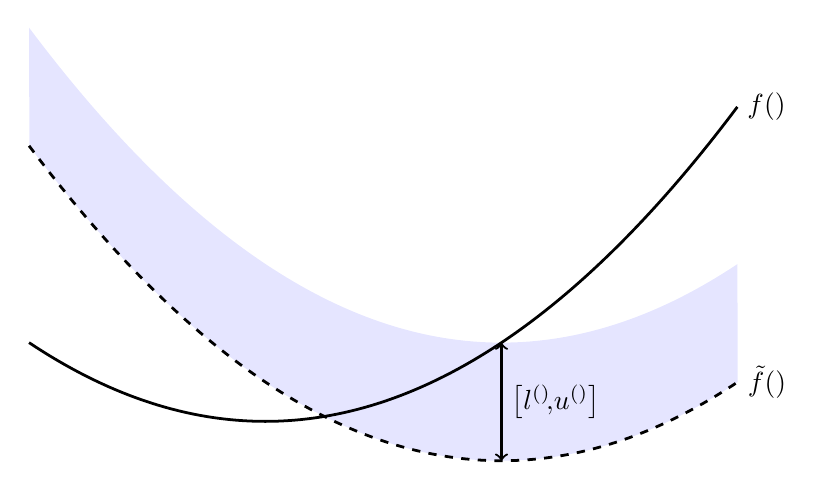
\begin{tikzpicture}[x=3cm, y=1cm]
 % Filled band around the quadratic curve with different boundary curves
\fill[blue!10] 
(-1, 5) -- plot[domain=-2:1, samples=100] ({\x+1}, {\x*\x + 1}) -- 
plot[domain=1:-2, samples=100] ({\x+1}, {\x*\x - 0.5}) -- cycle;
 \node[anchor=west] at (2, 4) {$f(\weights)$};
 \draw[line width=1, domain=-2:1, samples=100,dashed] plot  ({\x+1}, {\x*\x -0.5}) node[right] {$\tilde{f}(\weights)$};
  \draw[line width=1, domain=-1:2, samples=100] plot ({\x}, {\x*\x});
 \draw[<->, thick] (1, -0.5) -- (1, 1) node[midway, right] {$\big[ l^{(\weights)}\!,\!u^{(\weights)} \big]$};
\end{tikzpicture}
\caption{Los métodos de aprendizaje automático aprenden parametros del modelo $\weights$ usando una estimación de $f(\weights)$ como 
	aproximación del criterio de desempeño $\bar{f}(\weights)$. Usando un modelo de probabilidad, se pueden construir intervalos de confianza $\big[ l^{(\weights)},  u^{(\weights)} \big]$ 
	que contienen $\bar{f}(\weights)$ con alta probabilidad. La mejor medida plausible del desempeño para una elección especifica $\weights$ es $\tilde{f}(\weights) \defeq l^{(\weights)}$.} 
	\end{center}
		\end{figure}.
		\\
	 Vea también: \gls{ml}, \gls{modelparams}, \gls{erm}, \gls{loss}, \gls{dataset}, \gls{trainset}, \gls{risk}, \gls{hypothesis}, \gls{probmodel}, \gls{ucb},  },first={optimismo ante la incertidumbre},text={optimismo ante la incertidumbre} 
}

\newglossaryentry{empgraph}
{name={red de aprendizaje federado (red FL)},
	description={Una red federada\index{red de aprendizaje federado (red FL)} es un grafo no dirigido y ponderado, 
	cuyos nodos representan generadores de datos que buscan entrenar un modelo local (o personalizado). 
	Cada nodo de una red federada representa un dispositivo capaz de recopilar un conjunto de datos local
	y, a su vez, entrenar un modelo local. 
	Los métodos de aprendizaje federado aprenden una hipótesis local $\localhypothesis{\nodeidx}$ para
	cada nodo $\nodeidx \in \nodes$, de manera que incurra en una perdida baja sobre su conjnto de datos local.
	\\
	 Vea también: \gls{graph},  \gls{data}, \gls{model}, \gls{device}, \gls{localdataset}, \gls{localmodel}, \gls{fl}, \gls{hypothesis}  },first={red de aprendizaje federado (red FL)},text={red FL} 
 }

\newglossaryentry{norm}
{name={norma},
	description={Una norma\index{norma} es una función que asigna a cada elemento (vectorial) de un espacio 
		vectorial lineal un número real no negativo. Esta función debe ser homogénea, definida positiva y debe 
		cumplir la desigualdad triangular \cite{HornMatAnalysis}. },
	first={norma},text={norma} 
}

\newglossaryentry{dualnorm}
{name={norma dual},
description={Toda norma $\normgeneric{\cdot}{}$ definida en un espacio euclidiano $\mathbb{R}^{\dimlocalmodel}$ 
		tiene una norma dual asociada, denotada por $\normgeneric{\cdot}{*}$ y definida como 
		$\normgeneric{\vy}{*} \defeq \sup_{\norm{\vx}{} \le 1} \vy^{T} \vx$. 
		La nroma dual mide el mayor producto interno posible entre $\vy$ y cualquier vector 
		en la bola unitaria de la norma original. Para más detalles, véa 
		\cite[Sec.~A.1.6]{BoydConvexBook}.\\ 
		Véa también: \gls{norm}, \gls{euclidspace}.},
	first={norma dual},
	text={norma dual}
}

\newglossaryentry{geometricmedian}{
	name={mediana geométrica (GM)},
	description={La GM\index{mediana geométrica (GM)} de un conjunto de vectores de entrada 
	$\vx^{(1)}, \ldots, \vx^{(\samplesize)}$ en $\mathbb{R}^{\dimlocalmodel}$ 
	es un punto $\vz \in \mathbb{R}^{\dimlocalmodel}$ que minimiza la suma de distancias 
	a dichos vectores \cite{BoydConvexBook}, es decir:
	\begin{equation} 
		\label{equ_geometric_median_dict}
	\vz \in \argmin_{\vy \in \mathbb{R}^{\dimlocalmodel}} \sum_{\sampleidx=1}^{\samplesize} \normgeneric{\vy - \vx^{(\sampleidx)}}{2}.
	\end{equation} 
	La Figura~\ref{opt_cond_GM_dict} ilustra una propiedad fundamental de la GM:
	si $\vz$ no coincide con ninguno de los vectores de entrada, entonces los vectores unitarios 
	que apuntan desde $\vz$ hacia cada $\vx^{(\sampleidx)}$ deben sumar cero; 
	esta es la condición de \gls{subgradient} nulo (óptima) de \eqref{equ_geometric_median_dict}. 
	Además, se ha demostrado que la solución de \eqref{equ_geometric_median_dict} 
	no puede alejarse arbitrariamente de los vectores de entrada confiables 
	mientras estos constituyan la mayoría \cite[Th. 2.2]{Lopuhaae1991}.
	  	\begin{figure}[H]
  		\begin{center}
			\begin{tikzpicture}[scale=2, thick, >=stealth]
				\coordinate (w) at (3,0);
				\fill (w) circle (1.2pt) node[below right] {$\vz$};
				% Vectores limpios
				\coordinate (w2) at (0.5,0.3);
				\coordinate (w3) at (0.7,0.7);
				\fill (w2) circle (1pt) node[above left] {$\vx^{(1)}$};
				\fill (w3) circle (1pt) node[above left] {$\vx^{(2)}$};
			    \node[anchor=west] at ($(w2) +(-0.2,0.9)$) {\textbf{limpios}};
				% Líneas
				\draw[dashed] (w) -- (w2);
				\draw[dashed] (w) -- (w3);
				% Vectores unitarios
				\draw[->, thick, red] (w) -- ($(w)!1cm!(w2)$) ;
				\draw[->, thick, red] (w) -- ($(w)!1cm!(w3)$) node[pos=0.9, right,yshift=7pt] {$\frac{\vx^{(2)}- \vz}{\normgeneric{\vx^{(2)}-\vz}{2}}$};
				% Punto perturbado
				\coordinate (w4) at (5,0.2);
				\node at (5,0.6) {\textbf{perturbado}};
				\fill (w4) circle (1pt) node[below left] {$\vx^{(3)}$};
				\draw[->, thick, red] (w) -- ($(w)!1cm!(w4)$) ;
			\end{tikzpicture}
			\caption{\label{opt_cond_GM_dict}
			Sea $\vz$ una solución de \eqref{equ_geometric_median_dict} que no coincide con ninguno 
			de los vectores de entrada. La condición de optimalidad requiere que los vectores 
			unitarios desde $\vz$ hacia los vectores de entrada sumen cero.}
			\end{center}
	\end{figure}
	Véa también: \gls{subgradient}.
},
	first={mediana geométrica},
	text={GM}
}




\newglossaryentry{explanation}
{name={explicacion},
	description={
		Un enfoque para mejorar la transparencia de un método de aprendizaje automático para su usuario humano 
		es proporcionar una explicación\index{explanation} junto con las predicciones entregadas 
		por el método. Las explicaciones pueden adoptar diferentes formas. Por ejemplo, pueden 
		consistir en texto legible para humanos o indicadores cuantitativos, como puntuaciones de importancia 
		de los atributos para los atributos individuales de un punto de datos dado~\cite{Molnar2019}. 
		Alternativamente, las explicaciones pueden ser visuales, por ejemplo, mapas de intensidad que resaltan 
		las regiones de una imagen que impulsan la predicción \cite{GradCamPaper}. 
		La Fig.\ \ref{fig_explanation_dict} ilustra dos tipos de explicaciones. La primera 
		es una aproximación lineal local $g(\featurevec)$ de un modelo no lineal entrenado 
		$\learnthypothesis(\featurevec)$ alrededor de un \gls{featurevec} específico $\featurevec'$, 
		como se utiliza en el método lime. 
		La segunda forma de explicación representada en la figura es un conjunto disperso de predicciones
		$\learnthypothesis(\featurevec^{(1)}), \learnthypothesis(\featurevec^{(2)}), \learnthypothesis(\featurevec^{(3)})$ 
		en vectores de atributos seleccionados, que ofrecen puntos de referencia concretos para el usuario.
	 	 \begin{figure}[H]
	   		\begin{center}
	 		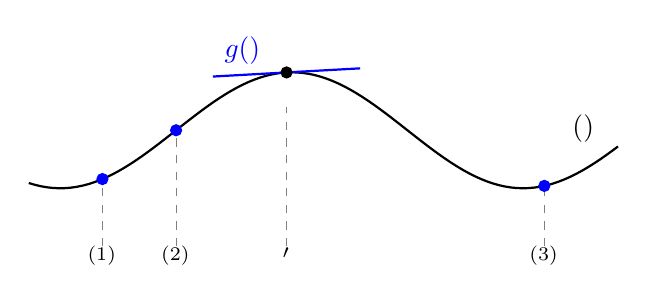
\begin{tikzpicture}[x=0.5cm]
	 		\begin{axis}[
	 			hide axis,
	 			xmin=-3, xmax=6,
	 			ymin=0, ymax=6,
	 			domain=0:6,
	 			samples=100,
	 			width=10cm,
	 			height=6cm,
	 			clip=false
	 		   ]
	 	% Original nonlinear function h(x)
			\addplot[thick, domain=-2:6] {2 + sin(deg(x))} 
	   		     node[pos=0.9, above right, yshift=10pt] {$\learnthypothesis(\featurevec)$};
	 	% Tangent line as local linear approximation at x = 1.5
	 	% h(3) = 2 + sin(3), h'(3) = cos(3)
	 		\addplot[blue, thick, domain=0.5:2.5] 
	 		{2 + sin(deg(1.5)) + cos(deg(1.5))*(x - 1.5)}
	 		node[pos=0.2, above] {$g(\featurevec)$};
	 	% Mark point of approximation
	 		\addplot[mark=*] coordinates {(1.5, {2 + sin(deg(1.5))})};
	 		    % Vertical dashed line (ruler) at x = 1.5
			\addplot[dashed, gray] coordinates {(1.5,0) (1.5,2.4)};
	 		\node at (axis cs:1.5, -0.2) {$\featurevec'$};
	      % add function values for finite set of featurevecs
	       \addplot[mark=*,blue] coordinates {(-1, {2 + sin(deg(-1))})};
	       	\addplot[dashed, gray] coordinates {(-1,0) (-1,{2 + sin(deg(-1))})};
	       \node at (axis cs:-1, -0.2) {$\featurevec^{(1)}$};
	 	   \addplot[mark=*,blue] coordinates {(0, {2 + sin(deg(0))})};
	 	   	\addplot[dashed, gray] coordinates {(0,0) (0,{2 + sin(deg(0))})};
	 	   \node at (axis cs:0, -0.2) {$\featurevec^{(2)}$};
	 	   \addplot[mark=*,blue] coordinates {(5, {2 + sin(deg(5))})};
	 	   	 	   	\addplot[dashed, gray] coordinates {(5,0) (5,{2 + sin(deg(5))})};
	 	   \node at (axis cs:5, -0.2) {$\featurevec^{(3)}$};
	% 		    % Plot the two points
	% 		    % Coordinates of the two points
	% 		\pgfmathsetmacro{\xA}{-1.5}
	% 		\pgfmathsetmacro{\xB}{3}
	% 		\pgfmathsetmacro{\yA}{2 + sin(deg(\xA))}
	% 		\pgfmathsetmacro{\yB}{2 + sin(deg(\xB))}
	 		\end{axis}
	% 	\vspace*{-10mm}
	 \end{tikzpicture}
	 \end{center}
	 \caption{Un modelo entrenado $\learnthypothesis(\featurevec)$ puede explicarse 
	 localmente en algún punto $\featurevec'$ mediante una aproximación lineal $g(\featurevec)$. 
	 Para un $\learnthypothesis(\featurevec)$ diferenciable, esta aproximación está 
	 determinada por el gradiente $\nabla \learnthypothesis(\featurevec')$. Otra 
	 forma de explicación podrían ser los valores de la funcion $\learnthypothesis\big(\featurevec^{(\sampleidx)} \big)$ 
	 para $\sampleidx=1,2,3$.
		\label{fig_explanation_dict}}
	 \end{figure} 
		Vea también: \gls{explainability}, \gls{trustAI}.},
	first={explicacion},
	text={explicacion} 
}

\newglossaryentry{risk}
{name={riesgo},
	description={Consideremos\index{riesgo} una hipótesis$\hypothesis$ que se utiliza para predecir la etiqueta 
		$\truelabel$ de un punto de datgos a partir de sus atributos $\featurevec$. Evaluamos 
		la calidad de una predicción específica usando una funcion de perdida $\lossfunc{(\featurevec,\truelabel)}{\hypothesis}$. 
		Si interpretamos los puntos de datos como realizaciónes de variabels aleatorias iid, 
		entonces $\lossfunc{(\featurevec,\truelabel)}{\hypothesis}$ también se convierte en una realización
		de una variable aleatoria. La suposición de independencia e idéntica distribución nos permite definir el riesgo de una hipótesis
		como la expectativa de la perdida $\expect \big\{\lossfunc{(\featurevec,\truelabel)}{\hypothesis} \big\}$. 
		El riesgo de $\hypothesis$ depende tanto de la funcion de perdida elegida como de la distribución de probabilidad de los puntos de datos.
		\\
		 Vea también: \gls{hypothesis}, \gls{label}, \gls{datapoint}, \gls{feature},  \gls{prediction}, \gls{lossfunc}, \gls{realization}, \gls{rv}, \gls{iid}, gls{realization}, \gls{rv}, \gls{iidasspt}, \gls{expectation}, \gls{loss}, \gls{probdist}},
	first={riesgo},text={riesgo} 
}

\newglossaryentry{actfun}
{name={función de activación},
	description={Cada neurona artificial dentro de una red neuronal artificial (RNA)\index{función de activación} se le asigna 
		una función de activación $\actfun(\cdot)$ que transforma una combinación ponderada de 
		sus entradas $\feature_{1},\ldots,\feature_{\nrfeatures}$ en un único valor de salida: 
		$a = \actfun\big(\weight_{1} \feature_{1}+\ldots+\weight_{\nrfeatures} \feature_{\nrfeatures} \big)$. 
		Cada neurona está parametrizada por los pesos $\weight_{1},\ldots,\weight_{\nrfeatures}$.
		\\
		 Vea también:\gls{ann}, \gls{weights}},
first={función de activación},text={función de activación} 
}

\newglossaryentry{distributedalgorithm}
{name={algoritmo distribuido},
	description={Un algoritmo distribuido distributed\index{algoritmo distribuido} es un algoritmo diseñado para 
		un tipo especial de computadora: una colección de dispositivos de cómputo interconectados (o nodos). 
		Estos dispositivos se comunican y coordinan sus cálculos locales intercambiando mensajes
		a través de una red \cite{IntroDistAlg,ParallelDistrBook}. A diferencia de un algoritmo clásico,
		que se ejecuta en un solo dispositivo, un algoritmo distribuido   
		se ejecuta de forma concurrente en múltiples dispositivos con capacidades de cómputo. 
		Cada ejecución involucra tanto cálculos locales como eventos de intercambio de mensajes. 
		Una ejecución genérica podría verse así: 
		\[
		\begin{array}{l}
			\text{Node 1: } {\rm input}_1, s_1^{(1)}, s_2^{(1)}, \ldots, s_{T_1}^{(1)}, {\rm output}_1; \\
			\text{Node 2: } {\rm input}_2, s_1^{(2)}, s_2^{(2)}, \ldots, s_{T_2}^{(2)}, {\rm output}_2; \\
			\quad \vdots \\
			\text{Node N: } {\rm input}_N, s_1^{(N)}, s_2^{(N)}, \ldots, s_{T_N}^{(N)}, {\rm output}_N.
		\end{array}
		\]
		Cadad dispositivo  $\nodeidx$ inicia con su entrada local y ejecuta una secuencia de 
		de cálculos intermedios $s_{\iteridx}^{(\nodeidx)}$ en instantes de tiempo discretos $\iteridx = 1, \dots, T_\nodeidx$. 
		Estos cálculos pueden depender tanto de cálculos previos locales como de mensajes recibidos de otros dispositivos.
		Uno de los usos clave de los algoritmos distribuidos es en aprendizaje federado, donde una red de 
		dispositivos colaboran para entrenar un modelo personalizado por dispositivo.. 
		\\
		 Vea también: \gls{algorithm}, \gls{algorithm}, \gls{device}, \gls{fl}  },
	first={algoritmo distribuido}, text={algoritmo distribuido}
}



\newglossaryentry{algorithm}
{name={algoritmo},
  description={Un\index{algoritmo} algoritmo es una especificación precisa y paso a paso de
    cómo producir una salida a partir de una entrada dada en un número finito de pasos computacionales \cite{Cormen:2022aa}. 
    Por ejemplo, un algoritmo para entrenar un modelo lineal describe explícitamente cómo
	transformar un conjunto de entrenamiento dado en parametros del modelo a través de una secuencia de pasos de gradiente. 
    Esta caracterización informal puede formalizarse rigurosamente mediante diferentes modelos matemáticos \cite{Sipser2013}. 
   	Un modelo simple de un algoritmo es una colección de ejecuciones posibles. Cada ejecución es una secuencia:
    $${\rm input},s_1,s_2,\ldots,s_T,{\rm output}$$ 
    que respeta las restricciones inherentes al ordenador que ejecuta el algoritmo.
	Los algoritmos pueden ser deterministas, donde cada entrada resulta únicamente en una sola ejecución,
	o aleatorios, donde las ejecuciones pueden variar probabilísticamente. Los algoritmos aleatorios 
	pueden analizarse modelando las secuencias de ejecución como resultados de experimentos aleatorios, 
	considerando el algoritmo como un proceso estocástico \cite{RandomizedAlgos,BertsekasProb,Gallager13}.
	Crucialmente, un algoritmo abarca más que solo un mapeo de entrada a salida; también incluye 
	los pasos computacionales intermedios $s_1,\ldots,s_T$. 
	%. In \textbf{online algorithms}, these intermediate computational steps  can dynamically incorporate additional input data as the execution progresses.
	\\
		Vea también: \gls{linmodel}, \gls{trainset}, \glspl{modelparam}, \gls{gradstep}, \gls{model} },
	first={algoritmo},text={algoritmo} 
}

\newglossaryentry{stochalgorithm}
{name={algoritmo estocástico}, 
 plural={algoritmos estocásticos},
	description={Un\index{algoritmo estocástico} algoritmo estocástico utiliza un mecanismo aleatorio 
		durante su ejecución. Por ejemplo, descenso por gradiente estocástico utiliza un subconjunto seleccionado aleatoriamente 
		de puntos de datos para calcular una aproximación del gradiente de una funcion objetivo. 
		Podemos representar un algoritmo estocástico mediante un proceso estocástico, 
		es decir, la secuencia de ejecución posible es el conjunto de resultados posibles de un experimento aleatorio 
		\cite{BertsekasProb}, \cite{RandomizedAlgos}, \cite{Gallager13}.\\ 
		Véa también: \gls{stochastic}, \gls{algorithm}, \gls{stochGD}, \gls{datapoint}, \gls{gradient}, 
		\gls{objfunc}, \gls{optmethod}, \gls{gdmethods}.
	},
	first={algoritmo estocástico},
	text={algoritmo estocástico}
}


\newglossaryentry{onlinelearning}
{name={aprendizaje en línea},
	description={
		Algunos métodos de aprendizaje automático \index{aprendizaje en línea} están diseñados para procesar 
		datos de forma secuencial, actualizando sus parametros del modelo a medida que nuevos 
		puntos de datos se vuelven disponibles—uno a la vez. Un ejemplo típico son los datos de 
		series temporales, como las temperaturas minimas y maximas diarias registradas 
		por una estación meteorológica de FMI. Estos valores forman una secuencia cronológica 
		de observaciones. En el aprendizaje en línea, la hipótesis (o sus parametros del modelo) 
		se refina incrementalmente con cada nuevo punto de datos observado, sin volver a visitar 
		los datos anteriores.\\ 
		Véa también: \gls{ml}, \gls{data}, \glspl{modelparam}, \gls{datapoint}, \gls{fmi}, \gls{hypothesis}, \gls{onlineGD}, \gls{onlinealgorithm}.
	},
	first={aprendizaje en línea},
	text={aprendizaje en línea}
}

\newglossaryentry{onlinealgorithm}
{name=algoritmo en línea,
	description={
		Un algoritmo en línea\index{algoritmo en línea} es un algoritmo que procesa datos de forma incremental,
		recibiendo elementos de datos uno por uno y tomando decisiones o generando salidas inmediatamente, sin tener acceso a toda la entrada desde el inicio \cite{HazanOCO,PredictionLearningGames}.
		A diferencia de un algoritmo fuera de línea, que dispone de toda la entrada desde el comienzo, un algoritmo en línea debe lidiar con la incertidumbre del futuro y no puede cambiar decisiones pasadas.
		Puede modelarse como una ejecución del tipo:
		$${\rm init},s_1,{\rm out}_{1},{\rm in}_{2},s_2,{\rm out}_{2},\ldots,{\rm in}_{T},s_T,{\rm out}_{T}.$$
		Cada ejecución comienza en un estado inicial y alterna entre cálculos, salidas y nuevas entradas.
		Un ejemplo importante en aprendizaje automático es el descenso por gradiente en línea, que actualiza los modelos de parametro conforme llegan nuevos puntos de datos.
		\\
		Vea también: \gls{algorithm}, \gls{data}, \gls{ml}, \gls{onlineGD}, \glspl{modelparam}, \gls{datapoint} },
	first={algoritmo en línea},text={algoritmo en línea}
}



%\newglossaryentry{transparency}
%{name={transparency},
%	description={Transparency\index{transparency} is a key requirement for 
%		trustworthy \gls{ai} \cite{HLEGTrustworhtyAI}. In the context of ML methods, 
%		such as \gls{erm}-based methods, transparency is mainly used synonymously 
%		for \gls{explainability} \cite{gallese2023ai,JunXML2020}. However, in the wide 
%		context of \gls{ai} systems, transparency also includes providing information 
%		about limitations and reliability of the \gls{ai} system. As a point in case, \gls{logreg} provides a 
%		quantitative measure of the reliability of a \gls{classification} in the form of the value $|\hypothesis(\featurevec)|$. 
%		Transparency also includes the user interface, by requiring to clearly indicate when a user is 
%		interaction with an \gls{ai} system. Another component of transparency is the documentation 
%		of the system’s purpose, design choices, and intended use cases \cite{Shahriari2017,DatasheetData2021,10.1145/3287560.3287596}. },
%	first={transparency},text={transparency} 
%}

\newglossaryentry{transparency}
{name={transparencia},
	description={La transparencia\index{transparency} es un requisito fundamental para una 
		inteligencia artificial confiable confiable \cite{HLEGTrustworhtyAI}. En aprendizaje automático,
		suele utilizarse como sinónimo de explicabilidad \cite{gallese2023ai,JunXML2020}
		pero en el contexto más amplio de sistemas de inteligencia artificial, 
		incluye también información sobre limitaciones, confiabilidad y uso previsto. 
		En sistemas de diagnóstico médico, se requiere informar el nivel de confianza de una prediccion.
		En aplicaciones financieras como la puntuación crediticia, las decisiones automatizadas basadas en inteligencia artificial
		deben ir acompañadas de explicaciones sobre los factores que influyeron en ellas, como el nivel de ingresos o el historial crediticio. These explanations 
		Estas explicaciones permiten que las personas (por ejemplo, un solicitante de crédito) comprendan y, 
		si es necesario, impugnen decisiones automatizadas.. 
		Algunos métodos de aprendizaje automático ofrecen transparencia de manera intrínseca. Por ejemplo, la regresión logística 
		permite interpretar la fiabilidad de una clasificación mediante el valor absoluto $|\hypothesis(\featurevec)|$. 
		Los árboles de decisión, también son consideradas transparentes porque generan reglas comprensibles para los humanos.
		\cite{rudin2019stop}.
		La transparencia también requiere que se informe explícitamente cuando una persona está interactuando con un sistema de inteligencia artificial.
		Por ejemplo, los chatbots impulsados por inteligencia artifical deben indicar claramente que no son humanos. 
		Además, la transparencia incluye documentación exhaustiva que detalle el propósito, las decisiones de diseño y los casos de uso previstos del sistema.
		Ejemplos de esto son las hojas de datos de modelos \cite{DatasheetData2021}
		 y las tarjetas de sistemas de inteligencia artifical \cite{10.1145/3287560.3287596}, 
		 que ayudan a los desarrolladores y usuarios a entender las limitaciones y aplicaciones adecuadas de un sistema de inteligencia artificial \cite{Shahriari2017}.
		 \\
		Vea también: \gls{trustAI}, \gls{ml}, \gls{ai}, \gls{prediction}, \gls{logreg}, \gls{classification}, \gls{decisiontree}, \gls{model} },
	first={transparencia}, text={transparencia} 
}


\newglossaryentry{sensattr}
{
	name=atributo sensible,
	description={
		El aprendizaje automático\index{atributo sensible} busca aprender una hipótesis que prediga la etiqueta de un punto de datos a partir de sus atributos.
		En algunas aplicaciones, es crucial garantizar que la salida del sistema no permita inferir atributos sensibles de los puntos de datos. 
		Qué se considera atributo sensible depende del dominio de aplicación y debe definirse explícitamente.
		\\
		Vea también: \gls{ml}, \gls{hypothesis}, \gls{label}, \gls{datapoint}, \gls{feature},  },
	first={atributo sensible},text={atributo sensible}
}

\newglossaryentry{sbm}
{
	name=modelo estocástico de bloques (SBM),
	description={
		El modelo estocástico de bloques (SBM)\index{modelo estocástico de bloques (SBM)} es un modelo generativo probabilístico para un grafo no dirigido $\graph = \big( \nodes, \edges \big)$ con conjunto de nodos $\nodes$ \cite{AbbeSBM2018}.
		En su forma básica, asigna aleatoriamente cada nodo $\nodeidx \in \nodes$ a un clúster $\clusteridx_{\nodeidx} \in \{1,\ldots,\nrcluster\}$.
		Cada par de nodos distintos se conecta con probabilidad $p_{\nodeidx,\nodeidx'}$ que depende únicamente de sus etiquetas $\clusteridx_{\nodeidx}$ y $\clusteridx_{\nodeidx'}$.
		La presencia de aristas entre pares de nodos es estadísticamente independiente.
		\\
		Vea también: \gls{model}, \gls{graph}, \gls{cluster}, \gls{probability}, \gls{label}  },
	first={modelo estocástico de bloques (SBM)},text={SBM}
}


\newglossaryentry{deepnet}
{name={red profunda},
	description={Una red profunda\index{deep net} es una red neuronal artificial (RNA) con un número (relativamente) grande 
	de capas ocultas. El aprendizaje profundo (deep learning) es un término general para los métodos de aprendizaje automático 
	que utilizan una red profunda como modelo  \cite{Goodfellow-et-al-2016}.
	\\
		Vea también: \gls{ann}, \gls{ml}, \gls{model} },
	first={red profunda},text={red profunda} 
}

\newcommand{\gaussiancenter}{3}

\newglossaryentry{baseline}
{name={referencia (baseline)},
    description={Consideremos\index{referencia (baseline)} un método de aprendizaje automático que produce una 
    hipótesis aprendida (o un modelo entrenado) $\learnthypothesis \in \hypospace$.
	Evaluamos la calidad del modelo entrenado  
	mediante el cálculo de la perdida promedio en un conjunto de prueba. Pero, ¿cómo saber si ese rendimiento es lo suficientemente bueno?
	¿Cómo saber si el modelo entrenado se acerca al óptimo y si tiene sentido o no invertir más recursos (como recopilación de datos o potencia computacional) para mejorarlo? 
    Para ello, es útil contar con un valor de referencia (o *baseline*) con el cual comparar el rendimiento  
    del modelo entrenado. Este valor puede provenir del rendimiento humano,
    como la tasa de error de dermatólogos que diagnostican cáncer mediante inspección visual de la piel \cite{SkinHumanAI}.
	Otra fuente de referencia puede ser un método de aprendizaje automático ya existente que, por alguna razón, no sea adecuado para la aplicación (por ejemplo, por ser computacionalmente costoso), pero cuya tasa de error en el conjunto de prueba puede servir como baseline.
	Un enfoque más fundamentado para construir una baseline es utilizar un modelo de probabilidad. En muchos casos, dado un modelo de probabilidad $p(\featurevec,\truelabel)$,  
    podemos determinar con precisión el minimo riesgo alcanzable entre todas las hipótesis (incluso aquellas que no pertenecen al espacio de hipótesis $\hypospace$) \cite{LC}. 
    Este minimo alcanzable se conoce como riesgo de Bayes y corresponde al riesgo  para la etiqueta  $\truelabel$ de un punto de datos, dados sus atributos $\featurevec$.
	Dado una funcion de perdida específica, el estimador de Bayes (si existe) está completamente determinado por la distribución de probabilidad $p(\featurevec,\truelabel)$ \cite[Cap. 4]{LC}. 
    Calcular el estimador de bayes y el rieso de bayes presenta dos desafíos principales:
    \begin{enumerate}[label=\arabic*)]
    	\item La distribución de probabilidad $p(\featurevec,\truelabel)$ es desconocida y debe estimarse.
    	\item Incluso si se conoce $p(\featurevec,\truelabel)$ calcular el 
		riesgo de Bayes puede ser computacionalmente muy costoso \cite{cooper1990computational}.
	\end{enumerate}
	Un modelo de probabilidad ampliamente utilizado es la distribución normal multivariante $\pair{\featurevec}{\truelabel} \sim \mathcal{N}({\bm \mu},{\bm \Sigma})$ 
para puntos de datos caracterizados por atributos y etiquetas numéricas.
En este caso, bajo la pérdida de error cuadrático, el estimador de bayes corresponde a la media posterior
$\mu_{\truelabel|\featurevec}$ de la etiqueta $\truelabel$, dado  
atributos $\featurevec$ \cite{LC,GrayProbBook}. El riesgo de bayes asociado es la 
varianza posterior
$\sigma^{2}_{\truelabel|\featurevec}$ (see Figure \ref{fig_post_baseline_dict}).
	\begin{figure}[H]
		\begin{center}
		\begin{tikzpicture}
			% Axes
			\draw[->] (-1,0) -- (7,0) node[right] {$\truelabel$}; % x-axis
			% Gaussian distribution centered at \gaussiancenter with variance 1
			\draw[thick,domain=-1:7,smooth,variable=\x] 
			  plot ({\x}, {2*exp(-0.5*((\x-\gaussiancenter)^2))});
			% Dashed line indicating the mean of the Gaussian
			\draw[dashed] (\gaussiancenter,0) -- (\gaussiancenter,2.5);
			\node[anchor=south] at ([yshift=-5pt] \gaussiancenter,2.5) {\small $\mu_{\truelabel|\featurevec}$};
			% Double arrow indicating the variance
			\draw[<->,thick] (\gaussiancenter-1,1) -- (\gaussiancenter+1,1.0);
			\node[anchor=west] at ([yshift=2pt] \gaussiancenter,1.2) {\small $\sigma_{\truelabel|\featurevec}$};
			% Posterior variance label
			%\node[anchor=south east] at (\gaussiancenter-0.5,1.8) {\small Posterior Variance};
			% x-axis marks with crosses
			  % x-axis marks with crosses
  			\foreach \x in {0.5} {
				\node[red] at (\x, 0) {\bf \large $\times$};
 			 }
  % h(x) label for the first cross
  			\node[anchor=north] at (0.5,-0.2) {\small $\learnthypothesis(\featurevec)$};
		  \end{tikzpicture}
		\end{center}
		\caption{Si los atributos y la etiqueta de un punto de datos siguen una distribución normal multivariante,  
		podemos alcanzar el minimo riesgo (bajo pérdida de error cuadrático) usando el estimador de bayes $\mu_{\truelabel|\featurevec}$ 
		para predecir la etiqueta $\truelabel$ de un punto datos con atributos $\featurevec$. El
		minimo riesgo es dada por la varianza posterior $\sigma^{2}_{\truelabel|\featurevec}$. Podemos 
		usar esta cantidad como baseline para evaluar la perdida promedia del modelo $\learnthypothesis$ entrenado. \label{fig_post_baseline_dict}}
	\end{figure}
	.\\
		Vea también: \gls{ml},  \gls{hypothesis}, \gls{model}, \gls{loss}, \gls{testset}, \gls{data}, \gls{probmodel}, \gls{minimum},  \gls{risk}, \gls{hypospace}, \gls{bayesrisk}, \gls{bayesestimator}, \gls{probdist}, \gls{mvndist}   },
    first={referencia (baseline)},text={referencia (baseline)}
}

\newglossaryentry{spectrogram}
{name={espectrograma},
	description={
		Un\index{espectrograma} espectrograma representa la distribución tiempo-frecuencia de la energía de una señal temporal $x(t)$.  
		Intuitivamente, cuantifica la cantidad de energía de la señal presentedentro de un segmento de tiempo específico 
		$[t_{1},t_{2}] \subseteq \mathbb{R}$ y en un intervalo de frecuencia $[f_{1},f_{2}]\subseteq \mathbb{R}$. 
		Formalmente, el espectrograma de una señal se define como el módulo al cuadrado de su transformada
		de Fourier de ventana corta (STFT, en inglés) \cite{cohen1995time}.
        La Figure \ref{fig:spectrogram_dict} muestra una señal temporal junto con su espectrograma. 
	\begin{figure}[H]
		\centering
		\includegraphics[width=0.8\textwidth]{../../assets/spectrogram.png}
		\caption{Izquierda: una señal temporal compuesta por dos pulsos gaussianos modulados. Derecha: representación de intensidad de su espectrograma.
		\label{fig:spectrogram_dict}}
	\end{figure}
		La representación de intensidad del espectrograma puede considerarse como una imagen de la señal. 
		Una estrategia sencilla para la clasificación de señales de audio consiste en introducir esta imagen en una 
		red profunda desarrollada originalmente para tareas de clasificación de imágenes y detección de objetos \cite{Li:2022aa}. 
		Conviene señalar que, además del espectrograma, existen otras representaciones alternativas para describir la distribución 
		tiempo-frecuencia de la energía de una señal \cite{TimeFrequencyAnalysisBoashash,MallatBook}. 
		\\
		Vea también: \gls{classification}, \gls{deepnet} }, 
	first={espectrograma},text={espectrograma} 
}

\newglossaryentry{graphclustering}
{name={agrupamiento en grafos},
	description={El agrupamiento en grafos\index{agrupamiento en grafos} tiene como objetivo agrupar puntos de datos que están representados como nodos de un grafo $\graph$.
		Las aristas del $\graph$ representan similitudes por pares entre los puntos de datos. 
		En algunos casos, es posible cuantificar el grado de estas similitudes mediante un peso de arista \cite{Luxburg2007,FlowSpecClustering2021}. 
		\\
		Vea también: \gls{clustering}, \gls{graph}, \gls{datapoint}, \gls{edgeweight} }, 
	first={agrupamiento en grafos},text={agrupamiento en grafos} 
}

\newglossaryentry{specclustering}
{name={agrupamiento espectral},
	description={El agrupamiento espectral \index{agrupamiento espectral} es una instancia particular del 
		agrupamiento en grafos, es decir, agrupa puntos de datos
		representados como los nodos $\nodeidx=1,\ldots,\nrnodes$ de un grafo $\graph$. 
		El agrupamiento espectral utiliza los vectores propios de la matriz laplaciana $\LapMat{\graph}$ 
		para construir vectores de atributos $\featurevec^{(\nodeidx)} \in \mathbb{R}^{\nrfeatures}$ 
		para cada nodo (es decir, para cada punto de datos) $\nodeidx=1,\ldots,\nrnodes$. Podemos utilizar estos vectores de atributos 
		como entrada para métodos de agrupammiento en el espacio euclidiano,como k-means
		o agrupamiento suave mediante modelo de mezcla gaussiana. Mas o menos, los vectores de atributos de los nodos 
		que pertenecen a un subconjunto bien conectado (o agrupamiento) de nodos en $\graph$ estan ubicados 
		cerca en el espacio euclidiano $\mathbb{R}^{\nrfeatures}$ (Vea la Figura \ref{fig_lap_mtx_specclustering_dict}). 
		\begin{figure}[H]
			\begin{center}
				\begin{minipage}{0.4\textwidth}
			\begin{tikzpicture}
				% Define the style for filled nodes
				\begin{scope}[every node/.style={circle, fill=black, inner sep=0pt, minimum size=0.3cm}]
					% Define nodes
					\node (1) at (0,0) {};
					\node (2) [below left=of 1, xshift=-0.2cm, yshift=-1cm] {};
					\node (3) [below right=of 1, xshift=0.2cm, yshift=-1cm] {};
					\node (4) [below=of 1, yshift=0.5cm] {}; % Isolated node
				\end{scope}
				% Draw edges
				\draw (1) -- (2);
				\draw (1) -- (3);
				% Add labels (separate from filled nodes)
				\node[above=0.2cm] at (1) {$\nodeidx=1$};
				\node[left=0.3cm] at (2) {$2$};
				\node[right=0.3cm] at (3) {$3$};
				\node[below=0.2cm] at (4) {$4$};
			\end{tikzpicture}
				\end{minipage} 
				\hspace*{5mm}
				\begin{minipage}{0.4\textwidth}
					\begin{equation} 
						\LapMat{\graph}\!=\!
						\begin{pmatrix} 
							2 & -1 & -1 & 0 \\ 
							-1 & 1 & 0 & 0 \\  
							-1 & 0 & 1 & 0 \\ 
							0 & 0 & 0 & 0 
						\end{pmatrix}\!=\!\mathbf{V} {\bm \Lambda} \mathbf{V}^{T}  
						\nonumber
					\end{equation} 
				\end{minipage}
				\vspace*{20mm}\\
				  \begin{minipage}{0.4\textwidth}
				\begin{tikzpicture}[scale=3]
%					% Axes
					\draw[->] (-0.2, 0) -- (1.2, 0) node[right] {$v^{(1)}_{\nodeidx}$};
					\draw[->] (0, -0.2) -- (0, 1.2) node[above] {$v^{(2)}_{\nodeidx}$};
%					
%					% Tailored tick marks and labels
%					\draw (0,0) node[below left] {$0$};
%					\draw (1/sqrt(3), 0) node[below] {$\frac{1}{\sqrt{3}}$} -- ++(0,0.05);
%					\draw (0, 1) node[left] {$1$} -- ++(0.05,0);
%					
%					 Data points
					\filldraw[blue] (0.577, 0) circle (0.03cm) node[above right] {$\nodeidx=1,2,3$};
					\filldraw[blue] (0.577, 0) circle (0.03cm); % Second point overlaps
					\filldraw[blue] (0.577, 0) circle (0.03cm); % Third point overlaps
					\filldraw[red] (0, 1) circle (0.03cm) node[above right] {$4$};
%					% Grid for reference
%					\draw[dashed, gray] (1/sqrt(3), 0) -- (1/sqrt(3), 1);
%					\draw[dashed, gray] (0, 1) -- (1, 1);
				\end{tikzpicture}
				\end{minipage} 
    		\begin{minipage}{0.4\textwidth}
										\begin{align}
											& \mathbf{V} = \big( \vv^{(1)},\vv^{(2)},\vv^{(3)},\vv^{(4)} \big) \nonumber \\
											&	\mathbf{v}^{(1)}\!=\!\frac{1}{\sqrt{3}} \begin{pmatrix} 1 \\ 1 \\ 1 \\ 0 \end{pmatrix}, \,
												\mathbf{v}^{(2)}\!=\!\begin{pmatrix} 0 \\ 0 \\ 0 \\ 1 \end{pmatrix} \nonumber 
												\end{align}
				\end{minipage} 
				\caption{\label{fig_lap_mtx_specclustering_dict} {\bf Arriba.} Izquierda: Un grafo no dirigido
					$\graph$ con cuatro nodos $\nodeidx=1,2,3,4$, donde cada nodo representa un punto de datos. Derecha: La matriz laplaciana
					$\LapMat{\graph}  \in \mathbb{R}^{4 \times 4}$ y su descomposición en valores propios 
					{\bf Abajo.} Izquierda: Un diagrama de dispersión de los puntos de datos usando los vectores de atributos
					$\featurevec^{(\nodeidx)} = \big( v^{(1)}_{\nodeidx},v^{(2)}_{\nodeidx} \big)^{T}$. 
					Derecha: Dos vectores propios $\vv^{(1)},\vv^{(2)} \in \mathbb{R}^{\nrfeatures}$ 
					correspondientes al valor propio $\lambda=0$ de la matriz laplaciana $\LapMat{\graph}$. 
					} 
			\end{center}
		\end{figure}
	\newpage. \\
	Vea también: \gls{clustering}, \gls{graphclustering}, \gls{datapoint}, \gls{graph}, \gls{eigenvector}, \gls{LapMat}, \gls{featurevec}, \gls{euclidspace}, \gls{kmeans}, \gls{softclustering}, \gls{gmm}, \gls{evd}, \gls{scatterplot}, \gls{eigenvalue},  }, 
	first={agrupamiento espectral},text={agrupamiento espectral} 
}
\newglossaryentry{flowbasedclustering}
{name={agrupamiento basado en flujo},
	description={El agrupamiento basado en flujo\index{agrupamiento basado en flujo} agrupa los nodos de un 
		grafo no dirigido aplicando el algoritmo de k-means sobre
		vectores de atributos específicos para cada nodo. Estos vectores de atributos construyen a partir de flujos de red entre nodos 
		fuente y destino seleccionados cuidadosamente \cite{FlowSpecClustering2021}.
		\\
	Vea también: \gls{clustering}, \gls{graph}, \gls{kmeans}, \gls{featurevec}}, 
	first={agrupamiento basado en flujo},text={agrupamiento basado en flujo} 
}



\newglossaryentry{esterr}
{name={error de estimación},
	description={Consideremos\index{error de estimación} varios puntos de datos, cada uno con un vector de atributos $\featurevec$ y una etiqueta
		$\truelabel$. En algunas aplicaciones, podemos modelar la relación entre el vector de atributos y la etiqueta
		de un punto de datos como $\truelabel = \bar{\hypothesis}(\featurevec) + \varepsilon$. Aquí $\bar{\hypothesis}$ 
		representa la hipótesis verdadera subyacente y $\varepsilon$ es un término de ruido que resume errores de modelado o etiquetado.
		El error de estimación incurrido por un método de aprendizaje que aprende una hipótesis $\widehat{\hypothesis}$, por ejemplo usando ERM, se define como 
		$\widehat{\hypothesis}(\featurevec) - \bar{\hypothesis}(\featurevec)$, para algún vector de atributos dado. 
		En un espacio de hipótesis paramétrico, donde las hipótesis se determinan mediante
		parametros del modelo $\weights$, podemos definir el error de estimación como  $\Delta \weights = \widehat{\weights} - \overline{\weights}$ \cite{kay,hastie01statisticallearning}.
		\\
	Vea también: \gls{datapoint}, \gls{featurevec}, \gls{label}, \gls{hypothesis}, \gls{ml}, \gls{erm}, \gls{hypospace}, \glspl{modelparam}  },
	first={error de estimación},text={error de estimación} 
}


\newglossaryentry{dob}
{name={grado de pertenencia},
	description={El grado de pertenencia\index{grado de pertenencia} es un número que indica en qué medida un punto de datos 
		pertenece a un clúster \cite[Ch. 8]{MLBasics}. Este grado puede interpretarse 
		como una asignación blanda (*soft*) al clúster.Los métodos de agrupamiento suave
		pueden codificar el grado de pertenencia mediante un número real en el intervalo $[0,1]$. 
		El agrupamiento rígido se obtiene como caso extremo, cuando el grado de pertenencia solo toma los valores $0$ o $1$.
		\\
		Vea también: \gls{datapoint}, \gls{cluster}, \Gls{softclustering}, \Gls{hardclustering} }, 
		first={grado de pertenencia},text={grado de pertenencia} 
}

\newglossaryentry{msee}
{name={error cuadrático medio de estimación (MSEE)},
	description={Consideremos\index{error cuadrático medio de estimación (MSEE)} un método de aprendizaje automático que aprende 
		parametros del modelo $\widehat{\weights}$ a partir de un conjunto de datos $\dataset$. 
		Si interpretamos los puntos de datos en $\dataset$ como realizaciónes iid de una variable aleatoria $\datapoint$, 
		definimos el error de estimación como $\Delta \weights \defeq \widehat{\weight} - \overline{\weights}$. 
		Aquí, $\overline{\weights}$ representa los verdaderos parámetros del modelo de la distribución de probabilidad 
		de $\datapoint$. El error cuadrático medio de estimación se define como la expectativa $\expect \big\{ \big\| \Delta \weights \big\|^{2} \big\}$ del cuadrado de la 
		norma euclidiana del error de estimación\cite{LC,kay}.
		\\
		Vea también: \gls{ml}, \glspl{modelparam}, \gls{dataset}, \gls{datapoint}, \gls{realization}, \gls{esterr}, \gls{probdist}, \gls{expectation}, \gls{norm} },
	first={error cuadrático medio de estimación (MSEE)},text={MSEE} 
}

\newglossaryentry{gtvmin}
{name={minimización de variación total generalizada (GTVMin)},
	description={La minimización de variación total generalizada (GTVMin)\index{minimización de variación total generalizada (GTVMin)} es una instancia de minimización del riesgo empírico regularizado
	que utiliza la variación total generalizada de los parametros del modelo locales como un regularizador \cite{ClusteredFLTVMinTSP}.
	\\
		Vea también: \gls{rerm}, \gls{gtv}, \glspl{modelparam}, \gls{regularizer} },
	first={minimización de variación total generalizada (GTVMin)},text={GTVMin} 
}

\newglossaryentry{regression}
{name={regresión},
	description={Los problemas de regresión\index{regresión} se centran en la predicción de una 
		etiqueta numérica basada únicamente en los atributos de un punto de datos \cite[Ch. 2]{MLBasics}.
		\\
		Vea también: \gls{label}, \gls{feature}, \gls{datapoint}},
	first={regresión},text={regresión} 
}

\newglossaryentry{acc}
{name={precisión (accuracy)},
	description={Consideremos\index{precisión (accuracy)} puntos de datos caracterizados por atributos $\featurevec \in \featurespace$ y 
		una etiqueta categórica $\truelabel$ que toma valores de un conjunto finito espacio de etiquetas $\labelspace$. La 
		precisión de una hipótesis $\hypothesis: \featurespace \rightarrow \labelspace$, cuando se aplica a los
		puntos de datos en un conjunto de datos $\dataset = \big\{ \big(\featurevec^{(1)}, \truelabel^{(1)} \big), \ldots, \big(\featurevec^{(\samplesize)},\truelabel^{(\samplesize)}\big) \big\}$, 
		se define como $1 - (1/\samplesize)\sum_{\sampleidx=1}^{\samplesize} \lossfunczo{\big(\featurevec^{(\sampleidx)},\truelabel^{(\sampleidx)}\big)}{\hypothesis}$ usando la $\bf 0/1$ loss $\lossfunczo{\cdot}{\cdot}$.
		\\
		Vea también:  \gls{datapoint}, \gls{feature}, \gls{hypothesis}, \gls{dataset},  \gls{zerooneloss} },
	first={precisión (accuracy)},text={precisión} 
}





\newglossaryentry{expert}
{name={experto},
	description={El aprendizaje automático\index{experto} tiene como objetivo aprender una hipótesis $\hypothesis$ que prediga con precisión la etiqueta
		de un punto de datos basado en sus atributos Medimos el error de prediccion utilizando una
		funcion de perdida. Idealmente, buscamos una hipótesis que incurra en la perdida mínima
		para cualquier punto de datos. Podemos hacer este objetivo más preciso mediante la suposición de independencia e idéntica distribución 
		y utilizando el riesgo de bayes como referencia (baseline) para la perdida promedio de una hipótesis. 
		Una manera alternativa de obtener una referencia es utilizar la hipótesis $\hypothesis'$ aprendida 
		por un método de aprendizaje automático existente. A esta hipótesis $\hypothesis'$ la denominamos experto \cite{PredictionLearningGames}. Los métodos de minimización de arrepentimiento aprenden una hipótesis
		que incurre en una perdida comparable a la del mejor experto \cite{PredictionLearningGames,HazanOCO}.
		\\
		Vea también: \gls{ml}, \gls{hypothesis}, \gls{label}, gls{datapoint}, \gls{feature}, \gls{prediction}, \gls{lossfunc}, \gls{loss}, \gls{datapoint}, \gls{iidasspt}, \gls{bayesrisk}, \gls{baseline}, \Gls{regret} },
	first={experto},text={experto} 
}

\newglossaryentry{nfl}
{name={aprendizaje federado en red (NFL)},
	description={El aprendizaje federado en red (NFL)\index{aprendizaje federado en red (NFL)} se refiere 
		a métodos que aprenden modelos personalizados de manera distribuida. Estos métodos aprenden a partir de conjuntos de datos locales 
		que están relacionados por una estructura de red intrínsica.
		\\
		Vea también: \gls{model}, \gls{localdataset}},
 first={aprendizaje federado en red (NFL)},text={NFL} 
}




\newglossaryentry{regret}
{name={arrepentimiento (regret)},
	description={El arrepentimiento\index{arrepentimiento (regret)} de una hipótesis $\hypothesis$ en relación con otra 
		hipótesis $\hypothesis'$, que sirve como referencia, 
		es la diferencia entre la perdida incurrida por $\hypothesis$ y la perdida 
		incurrida por $\hypothesis'$ \cite{PredictionLearningGames}. 
		La hipótesis de referencia $\hypothesis'$ también se denomina experto.
		\\
		Vea también: \gls{hypothesis}, \gls{baseline}, \gls{loss}, \gls{expert}},
	first={arrepentimiento (regret)},text={arrepentimiento (regret)} 
}

\newglossaryentry{strcvx}
{name={fuertemente convexa},
	description={Una función real diferenciable de valor continuo 
		 $f(\featurevec)$es fuertemente convexa con coeficiente $\sigma$ si cumple: $f(\vy) \geq f(\vx) + \nabla f(\vx)^{T} (\vy - \vx) + (\sigma/2) \normgeneric{\vy - \vx}{2}^{2}$ \cite{nesterov04},\cite[Sec. B.1.1]{CvxAlgBertsekas}.
		 \\
		Vea también: \gls{differentiable}, \gls{convex}},
	first={fuertemente convexa},text={fuertemente convexa} 
}

\newglossaryentry{differentiable}
{name={diferenciable},
	description={Una función real $f: \mathbb{R}^{\featuredim} \rightarrow \mathbb{R}$ 
		es diferenciable\index{diferenciable} si, en cualquier punto, puede aproximarse localmente mediante una función lineal.
		La aproximación lineal local en el punto $\mathbf{x}$ es determinada por el 
		gradiente $\nabla f ( \mathbf{x})$ \cite{RudinBookPrinciplesMatheAnalysis}.
		\\
		Vea también: \gls{gradient}},
	first={diferenciable},text={diferenciable} 
}

\newglossaryentry{gradient}
{name={gradiente},
	description={Para\index{gradiente} una función de valor real $f: \mathbb{R}^{\featuredim} \rightarrow \mathbb{R}: \weights \mapsto f(\weights)$, 
	un vector $\vg$ tal que $\lim_{\weights \rightarrow \weights'} \frac{f(\weights) - \big(f(\weights')+ \vg^{T} (\weights- \weights') \big) }{\| \weights-\weights'\|}=0$ 
	se denomina gradiente de $f$ en $\weights'$. Si existe tal vector, se denota como
	$\nabla f(\weights')$ o $\nabla f(\weights)\big|_{\weights'}$ \cite{RudinBookPrinciplesMatheAnalysis}.
	},
	first={gradiente},text={gradiente} 
}

\newglossaryentry{subgradient}
{name={subgradiente},
description={Para\index{subgradiente} una función de valor real $f: \mathbb{R}^{\featuredim} \rightarrow \mathbb{R}: \weights \mapsto f(\weights)$, 
		un vector $\va$ tal que $f(\weights) \geq  f(\weights') +\big(\weights-\weights' \big)^{T} \va$ se 
		se denomina subgradiente de $f$ en $\weights'$ \cite{BertCvxAnalOpt,BertsekasNonLinProgr}.},
	first={subgradiente},text={subgradiente} 
}



\newglossaryentry{fedprox}
{name={FedProx},
	description={FedProx\index{FedProx}  se refiere a un algoritmo iterativo de aprendizaje federado que alterna entre entrenar modelos locales por separado y combinar los parametros del modelo locales actualizados. 
		A diferencia del promedio federado, que utiliza descenso de gradiente estocástico para entrenar los modelos locales, FedProx usa un operador proximal para el entrenamiento \cite{FedProx2020}.
		\\
		Vea también: \gls{algorithm}, \gls{localmodel}, \glspl{modelparam}, \gls{fedavg}, \gls{stochGD}, \gls{proxop} }, 
	first = {FedProx}, text={FedProx} 
}

\newglossaryentry{relu}
{name={unidad lineal rectificada (ReLU)},
	description={La unidad lineal rectificada (ReLU)\index{unidad lineal rectificada (ReLU)} es una elección popular para la 
		función de activación de una neurona dentro de una red neuronal artificial. Se define como  
		$\actfun(z) = \max\{0,z\}$, donde $z$ es la entrada ponderada de la neurona artificial.
		\\
		Vea también: \gls{actfun}, \gls{ann}}, 
	first = {unidad lineal rectificada (ReLU)}, text={ReLU} 
}

\newglossaryentry{hypothesis}
{name={hipótesis},
	description={Una hipótesis\index{hipótesis} se refiere a un mapa (o función) $\hypothesis: \featurespace \rightarrow \labelspace$ que va del
		espacio de atributos $\featurespace$ al espacio de etiquetas $\labelspace$. 
		Dado un punto de datos con atributos $\featurevec$, utilizamos un mapa de hipótesis $\hypothesis$
		para estimar (o aproximar) la etiqueta $\truelabel$ mediante la prediccion
		$\hat{\truelabel} = \hypothesis(\featurevec)$. El aprendizaje automático se centra en aprender (o encontrar) un mapa de hipótesis 
		$\hypothesis$ tal que $\truelabel \approx \hypothesis(\featurevec)$ 
		para cualquier punto de datos (con atributos $\featurevec$ y etiqueta $\truelabel$).
		\\
		Vea también: \gls{labelspace}, \gls{datapoint}, \gls{feature}, \gls{label}, \gls{prediction}, \Gls{ml}  },
	first={hipótesis},text={hipótesis}  
}



\newglossaryentry{vcdim}
{name={dimensión de Vapnik–Chervonenkis (dimensión VC)},
description={La\index{dimensión de Vapnik–Chervonenkis (dimensión VC)} dimensión VC 
	es una medida ampliamente utilizada para cuantificar el tamaño de un espacio de hipótesis infinito. 
	Remitimos a la literatura (véa \cite{ShalevMLBook}) para una definición precisa 
	de la dimensión VC, así como una discusión sobre sus propiedades básicas y su uso en aprendizaje automatico.
			\\ 
	Vea tambien: \gls{hypospace}, \gls{ml}, \gls{effdim}.},
first={dimensión de Vapnik–Chervonenkis (dimensión VC)},
text={dimensión VC}  
}


\newglossaryentry{effdim}
{name={dimensión efectiva},
	description={La dimensión efectiva\index{dimensión efectiva} $\effdim{\hypospace}$ de un 
		espacio de hipótesis infinito $\hypospace$ es una medida de su tamaño. A grandes rasgos,la 
		dimensión efectiva es igual al número efectivo de parametros del modelo independientes y ajustables. 
		Estos parametros pueden ser los coeficientes utilizados en un mapa lineal o los 
		pesos y términos de sesgo de una red neuronal artificial.
		\\
		Vea también: \gls{hypospace}, \glspl{modelparam}, \gls{parameters}, \gls{weights}, \gls{ann} },
	first={dimensión efectiva},text={dimensión efectiva}  
}

\newglossaryentry{labelspace}
{name={espacio de etiquetas},
	description={Consideremos\index{espacio de etiquetas} una aplicación de aprendizaje automático que involucra puntos de datos caracterizados por atributos
		y etiquetas. El espacio de etiquetas está constituido por todos los valores potenciales que una etiqueta
		de un punto de datos puede asumir. Los métodos de regresión, que buscan predecir etiquetas numéricas 
		a menudo utilizan el espacio de etiquetas $\labelspace = \mathbb{R}$. Los métodos de clasificación binaria utilizan un espacio de etiquetas  
		que consiste de dos elementos diferentes, por ejemplo, $\labelspace =\{-1,1\}$, $\labelspace=\{0,1\}$, 
		o $\labelspace = \{ \mbox{``imagen de gato''}, \mbox{``sin imagen de gato''} \}$.
		\\
		Vea también: \gls{ml}, \gls{datapoint},  \gls{feature}, \gls{label}, \Gls{regression}, \gls{classification} }, 
		first={espacio de etiquetas},text={espacio de etiquetas}  
}

\newglossaryentry{prediction}
{name={predicción},
	description={Una \index{prediction} predicción es una estimación o aproximación de una cantidad de interés.  
		El Aprendizaje Automático se centra en aprender o encontrar un mapa de hipótesis $\hypothesis$ 
		que recibe los atributos $\featurevec$ de un punto datos and y produce una predicción
		$\widehat{\truelabel} \defeq \hypothesis(\featurevec)$ para su etiqueta $\truelabel$. 
		\\
		Vea también:  \Gls{ml}, \gls{hypothesis}, \gls{feature}, \gls{datapoint}},
	first={predicción},text={predicción}  
}
\newglossaryentry{histogram}
{name={histograma},
	description={Considere\index{histograma} un conjunto de datos $\dataset$ que consiste en $\samplesize$ puntos de datos
		$\datapoint^{(1)}, \ldots, \datapoint^{(\samplesize)}$, cada uno perteneciente a una 
		celda $[-U,U] \times \ldots \times [-U,U] \subseteq \mathbb{R}^{\featuredim}$ con longitud 
		lateral $U$. Particionamos esta celda de manera uniforme en celdas elementales más pequeñas con longitud 
		lateral $\Delta$. El histograma de $\dataset$ asigna a cada celda elemental la fracción correspondiente de puntos de datos
		en $\dataset$ que caen dentro de dicha celda elemental. Un ejemplo visual de tal histograma se muestra en la Fig. \ref{fig:histogram_dict}.\\
		\begin{figure}[H]
		\centering
		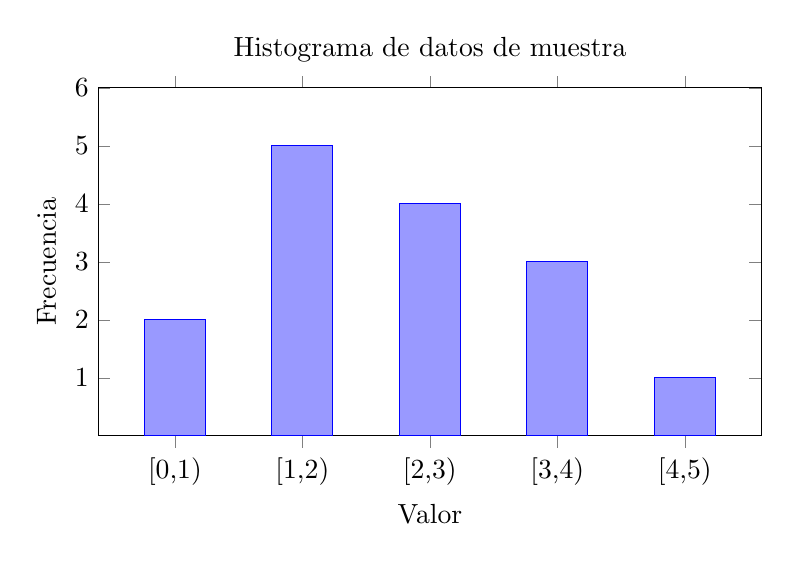
\begin{tikzpicture}
		\pgfplotsset{compat=1.18}
		\begin{axis}[
		    ybar,
		    ymin=0,
		    ymax=6,
		    bar width=22pt,
		    width=10cm,
		    height=6cm,
		    xlabel={Valor},
		    ylabel={Frecuencia},
		    ytick={1,2,3,4,5,6},
		    xtick={1,2,3,4,5},
		    xticklabels={{[0,1)}, {[1,2)}, {[2,3)}, {[3,4)}, {[4,5)}},
		    enlarge x limits=0.15,
		    title={Histograma de datos de muestra}
			]
		\addplot+[fill=blue!40] coordinates {(1,2) (2,5) (3,4) (4,3) (5,1)};
		\end{axis}
		\end{tikzpicture}
		\caption{Un histograma que representa la frecuencia de puntos de datos que caen dentro de rangos de valores discretos (es decir, intervalos). 
		La altura de cada barra muestra la cantidad de muestras en el intervalo correspondiente.}
		\label{fig:histogram_dict}
		\end{figure}
		Véa también: \gls{dataset}, \gls{datapoint}, \gls{sample}.},
	first={histograma},
	text={histograma}  
}


\newglossaryentry{bootstrap}
{name={bootstrap},
	description={Para\index{bootstrap} el análisis de métodos de aprendizaje automático, es a menudo útil interpretar 
		un conjunto dado de puntos de datos $\dataset = \big\{ \datapoint^{(1)},\ldots,\datapoint^{(\samplesize)}\big\}$ 
		como realizaciónes de variables aleatorias iid con una distribución de probabilidad común $p(\datapoint)$. En general, no conocemos 
		$p(\datapoint)$ exactamente, por lo que necesitamos estimarla. El método bootstrap utiliza el histograma de 
		$\dataset$ como un estimador para la distribución de probabilidad subyacente $p(\datapoint)$. 
		\\
		Vea también: \gls{ml}, \gls{datapoint}, \gls{realization}, \gls{rv}, \gls{iid},\gls{probdist} },
	first={bootstrap},text={bootstrap}  
}


\newglossaryentry{featurespace}
{name={espacio de atributos},
	description={El\index{espacio de atributos} espacio de atributos de una determinada aplicación 
	o método de aprendizaje automático está constituido por todos los valores posibles que puede tomar el vector de atributos de un 
	punto de datos.
	\begin{figure}[H]
\centering
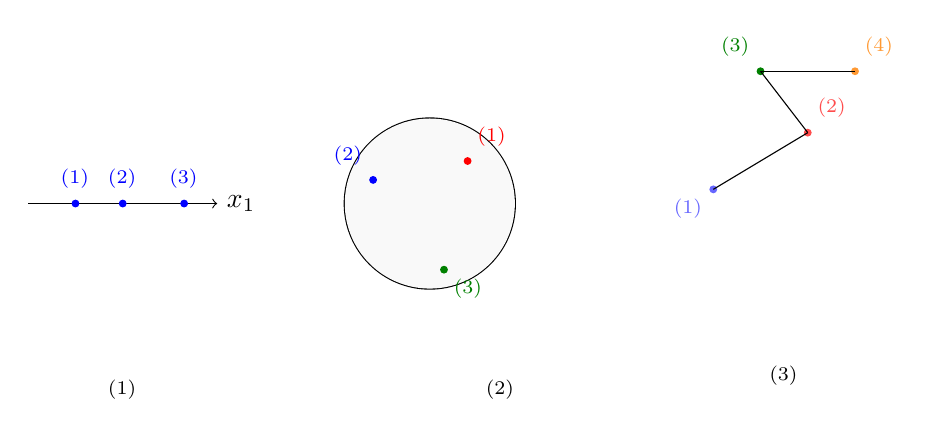
\begin{tikzpicture}[scale=0.6]
% --------- 1D Line Feature Space (left) ---------
\begin{scope}[xshift=0cm]
  % Axis
  \draw[->] (-0.5, 0) -- (3.5, 0) node[right] {$x_1$};
  % Points
  \foreach \x/\lbl in {0.5/$\featurevec^{(1)}$, 1.5/$\featurevec^{(2)}$, 2.8/$\featurevec^{(3)}$}
    \filldraw[blue] (\x,0) circle (2pt) node[above] {\lbl};
  % Label
  \node at (1.5, -4.0)  {$\featurespace^{(1)}$};
\end{scope}
% --------- 2D Bounded (Disk) Feature Space (middle) ---------
\begin{scope}[xshift=8cm]
  % Circle boundary
  \draw[thick] (0,0) circle (1.8);
  \fill[gray!5] (0,0) circle (1.8);
  % Points inside circle
  \filldraw[red] (0.8, 0.9) circle (2pt) node[anchor=south west] {$\featurevec^{(1)}$};
  \filldraw[blue] (-1.2, 0.5) circle (2pt) node[anchor=south east] {$\featurevec^{(2)}$};
  \filldraw[green!50!black] (0.3, -1.4) circle (2pt) node[anchor=north west] {$\featurevec^{(3)}$};
  % Label
  \node at (1.5, -4) {$\featurespace^{(2)}$};
\end{scope}
% --------- Graph-Based Feature Space (right) ---------
\begin{scope}[xshift=14cm, yshift=0.3cm]
  % Nodes
  \filldraw[blue!60] (0,0) circle (2pt) node[anchor=north east] {$\featurevec^{(1)}$};
  \filldraw[red!70] (2,1.2) circle (2pt) node[anchor=south west] {$\featurevec^{(2)}$};
  \filldraw[green!50!black] (1,2.5) circle (2pt) node[anchor=south east] {$\featurevec^{(3)}$};
  \filldraw[orange!80] (3,2.5) circle (2pt) node[anchor=south west] {$\featurevec^{(4)}$};
  % Edges
  \draw[-] (0,0) -- (2,1.2);
  \draw[-] (2,1.2) -- (1,2.5);
  \draw[-] (1,2.5) -- (3,2.5);
  % Label
  \node at (1.5, -4.0) {$\featurespace^{(3)}$};
\end{scope}
\end{tikzpicture}
\caption{Tres espacios de atributos distintos: un espacio lineal $\featurespace^{(1)} = \mathbb{R}$, 
un conjunto convexo acotado $\featurespace^{(2)} \subseteq \mathbb{R}^{2}$, y un espacio discreto 
$\featurespace^{(3)}$ cuyos elementos son nodos de un grafo no dirigido.}
\end{figure}
Para puntos de datos descritos por un número fijo $\nrfeatures$ de atributos numéricos, 
una elección común para el espacio de atributos es el espacio euclidiano $\mathbb{R}^{\nrfeatures}$. 
Sin embargo, la mera presencia de $\nrfeatures$ atributos numéricos no implica que 
$\mathbb{R}^{\nrfeatures}$ sea la representación más adecuada del espacio de atributos. 
De hecho, los atributos numéricos podrían asignarse a los puntos de datos de forma mayormente arbitraria o aleatoria, 
lo que da lugar a puntos de datos dispersos al azar en $\mathbb{R}^{\nrfeatures}$ 
sin una estructura geométrica significativa. Los métodos de aprendizaje de atributos intentan aprender 
una transformación de los atributos originales (potencialmente no numéricos) que permita 
una disposición más significativa de los puntos de datos en $\mathbb{R}^{\nrfeatures}$.\\
		Véa también: \gls{featurevec}, \gls{euclidspace}.},
	first={espacio de atributos},
	text={espacio de atributos}  
}



\newglossaryentry{missingdata}
{name={datos faltantes},
	description={Considere\index{datos faltantes} un conjunto de datos constituido por puntos de datos recopilados  
		a través de algún dispositivo físico. Debido a imperfecciones y fallas, algunos de los valores de atributos
		o etiquetas de los puntos ded atos podrían estar corruptos o simplemente faltar.  
		La imputación de datos tiene como objetivo estimar estos valores faltantes \cite{Abayomi2008DiagnosticsFM}. 
		Podemos interpretar la imputación de datos como un problema de aprendizaje automático donde la etiqueta de un punto de datos es 
		es el valor del atributo corrupto. 
		\\
		Vea también:  \gls{dataset}, \gls{datapoint}, \gls{device}, \gls{feature}, \gls{label}, \gls{datapoint}, \Gls{data} },
	first={datos faltantes},text={datos faltantes}  
}


\newglossaryentry{psd}
{name={semi-definida positiva (psd)},
    description=
    {Una \index{semi-definida positiva (psd)} matriz simétrica (con valores reales) $\mQ = \mQ^{T} \in \mathbb{R}^{\featuredim \times \featuredim}$ 
	se denomina semi-definida positiva (psd) si $\featurevec^{T} \mQ \featurevec \geq 0$ para todo vector $\featurevec \in \mathbb{R}^{\featuredim}$. 
	La propiedad de ser semi-definida positiva puede extenderse desde matrices a funciones kernel simétricas (con valores reales) 
	$\kernel: \featurespace \times \featurespace \rightarrow \mathbb{R}$ 
	(con $\kernel(\featurevec,\featurevec') = \kernel(\featurevec',\featurevec)$)
	de la siguiente manera: Para cualquier conjunto finito de vectores de atributos $\featurevec^{(1)},\dots,\featurevec^{(\samplesize)}$, 
	la matriz resultante $\mQ \in \mathbb{R}^{\samplesize \times \samplesize}$ con 
	entradas $Q_{\sampleidx,\sampleidx'} = \kernelmap{\featurevec^{(\sampleidx)}}{\featurevec^{(\sampleidx')}}$ 
	es semi-definida positiva \cite{LearningKernelsBook}.
	\\
		Vea también: \gls{kernel}, \gls{featurevec}},
    first={semi-definida positiva (psd)},text={psd}  
}

\newglossaryentry{feature}
{name={atributo},
	description={Un\index{atributo} atributo de un punto de datos es una de sus propiedades que se puede 
		medir o calcular fácilmente sin la necesidad de supervisión humana. Por ejemplo, si un punto de datos
		es una imagen digital (por ejemplo, almacenada como un archivo \texttt{.jpeg}), entonces podríamos usar
		las intensidades rojo-verde-azul de sus píxeles como atributos. Sinónimos específicos del dominio  
		para el término atributo incluyen "covariable", "variable explicativa", "variable independiente", "variable de entrada", "predictor (variable)" o "regresor" \cite{Gujarati2021}, \cite{Dodge2003}, \cite{Everitt2022}. 
		\\
		Vea también: \gls{datapoint} }, 
		first={atributo},text={atributo}  
}

\newglossaryentry{featurevec}
{
	name={vector de atributos},
	description={
		El\index{vector de atributos} vector de atributos se refiere a un vector 
		$\vx = \big(x_{1},\ldots,x_{\nrfeatures}\big)^{T}$ cuyos elementos son atributos individuales 
		$x_{1},\ldots,x_{\nrfeatures}$. 
		Muchos métodos de aprendizaje automático utilizan vectores de atributos que pertenecen a algún 
		espacio euclidiano de dimensión finita $\mathbb{R}^{\nrfeatures}$. Sin embargo, para algunos 
		métodos de aprendizaje automático, puede ser más conveniente trabajar con vectores de atributos que pertenezcan 
		a un espacio vectorial de dimensión infinita (por ejemplo, ver método de kernel). 
		\\
		Vea también: \gls{ml}, \gls{euclidspace}, \gls{ml}, \gls{kernelmethod}},
	first={vector de atributos},text={vector de atributos}  
}

\newglossaryentry{label}
{
	name={etiqueta},
	description={
		Una\index{etiqueta} es un hecho de nivel superior o una cantidad de interés asociada a un punto de datos. 
		Por ejemplo, si el punto de datos es una imagen, la etiqueta podría indicar si la 
		imagen contiene un gato o no. Los sinónimos de etiqueta, comúnmente utilizados en dominios específicos, 
		incluyen "variable de respuesta", "variable de salida" y "objetivo" \cite{Gujarati2021}, \cite{Dodge2003}, \cite{Everitt2022}.
		\\
		Vea también: \gls{datapoint}},
	first={etiqueta},text={etiqueta}  
}

\newglossaryentry{data}
{
	name={datos},
	description={
		Los\index{datos} datos se refieren a objetos que llevan información. 
		Estos objetos pueden ser tanto objetos físicos concretos (como personas o animales) 
		como conceptos abstractos (como números). 
		A menudo, utilizamos representaciones (o aproximaciones) de los datos originales que son 
		más convenientes para su procesamiento. Estas aproximaciones se basan en diferentes 
		modelos de datos, siendo el modelo de datos relacional uno de los más utilizados \cite{codd1970relational}.
	}, 
	text={datos}
}


\newglossaryentry{dataset}
{name={conjunto de datos},
	description={Un\index{conjunto de datos} conjunto de datos se refiere a una colección de puntos de datos. Estos 
		puntos de datos contienen información sobre alguna cantidad de interés (o etiqueta) dentro 
		de una aplicación de aprendizaje automático. Los métodos de aprendizaje automático utilizan conjuntos de datos para el entrenamiento de un modelo (por ejemplo, a través de ERM)
		y para la validación de modelos. Nuestra noción de conjunto de datos es muy flexible, 
		ya que permite diferentes tipos de puntos de datos. De hecho, los puntos de datos pueden ser objetos físicos concretos
		(como humanos o animales) o objetos abstractos (como números).
		Como ejemplo, la Figura\ \ref{fig_cows_dataset_dict} muestra un conjunto de datos que consiste en vacas como 
		punto de datos. 
		\begin{figure}[H]
				\begin{center}
		\label{fig:cowsintheswissalps_dict}
		\includegraphics[width=0.5\textwidth]{../../assets/CowsAustria.jpg}
		  \end{center}
		\caption{\label{fig_cows_dataset_dict} La manada de vacas}
	  \end{figure}
	   Con frecuencia, un ingeniero de aprendizaje automático no tiene acceso directo a un conjunto de datos. De hecho, acceder al conjunto de datos en la Figura 
        \ref{fig_cows_dataset_dict} requeriría visitar el rebaño de vacas en los Alpes. En su lugar, 
	   necesitamos utilizar una aproximación (o representación) del conjunto de datos que sea más conveniente para trabajar. 
       Se han desarrollado diferentes modelos matemáticos para la representación (o aproximación) de conjuntos de datos  
       \cite{silberschatz2019database}, \cite{abiteboul1995foundations}, \cite{hoberman2009data}, \cite{ramakrishnan2002database}. 
	   Uno de los modelos de datos más adoptados es el modelo relacional, que organiza los datos
       en una tabla (o relación) \cite{codd1970relational}, \cite{silberschatz2019database}.
	   Una tabla se compone de filas y columnas:
		\begin{itemize} 
		\item Cada fila de la tabla representa un solo punto de datos.
		\item Cada columna de la tabla corresponde a un atributo específico del punto de datos. 
		Los métodos de aprendizaje automático pueden utilizar estos atributos como atributos y etiquetas del punto de datos.
		\end{itemize}
		Por ejemplo, la Tabla \ref{tab:cowdata_dict} muestra una representación del conjunto de datos en la Figura. \ref{fig_cows_dataset_dict}. 
		En el modelo relacional, el orden de las filas es irrelevante, y cada atributo (es decir, columna) debe estar definido de manera precisa con un dominio, que especifica el conjunto de valores posibles.
		En las aplicaciones de aprendizaje automático, estos dominios de atributos se convierten en el espacio de atributos y el espacio de etiquetas. 
		\begin{table}[H]
			\refstepcounter{table}
			\caption*{
				\centering 
				\scshape TABLE \thetable \\[0.5ex]
				\scshape A Relation (or Table) That Represents the Dataset in Fig. \ref{fig_cows_dataset_dict} 
			}
			\label{tab:cowdata_dict} 
			\centering
			\begin{tabular}{lcccc}
				\hline
				\textbf{Name} & \textbf{Weight} & \textbf{Age} & \textbf{Height} & \textbf{Stomach temperature} \\
				\hline
				Zenzi & 100 & 4 & 100 & 25 \\
				Berta & 140 & 3 & 130 & 23 \\
				Resi  & 120 & 4 & 120 & 31 \\
				\hline
			\end{tabular}
		\end{table}
 Si bien el modelo relacional es útil para el estudio de muchas aplicaciones de aprendizaje automático, puede ser insuficiente 
 para cumplir con los requisitos de IA confiable. Enfoques modernos como las hojas de datos para conjuntos de datos proporcionan una documentación más completa,   
 incluyendo detalles sobre el proceso de recolección del conjunto de datos, su uso previsto y otra información contextual 
 \cite{DatasheetData2021}.
 \\
		Vea también: \gls{datapoint}, \gls{label}, \gls{ml}, \gls{model},  \gls{erm}, \gls{validation}, \gls{data}, \gls{featurespace}, \gls{labelspace}, \gls{trustAI}},first={conjunto de datos},text={conjunto de datos}  
}

\newglossaryentry{predictor}
{name={predictor},
	description={Un\index{predictor} predictor es un mapa de hipótesis con valores reales.
		Dado un punto de datos con atributos $\featurevec$, el valor 
		$\hypothesis(\featurevec) \in \mathbb{R}$ se utiliza como una predicción para la verdadera  
		etiqueta numérica $\truelabel \in \mathbb{R}$ del punto de datos. 
		\\
		Vea también: \gls{hypothesis}, \gls{datapoint}, \gls{feature}, \gls{prediction}, \gls{label} },first={predictor},text={predictor}  
}

\newglossaryentry{labeled datapoint}
{name={punto de dato etiquetado},
 description={Un\index{punto de dato etiquetado} punto de datos cuya etiqueta es conocida o ha sido determinada  
 por algún medio, lo que podría requerir trabajo humano.
 \\
	Vea también: \gls{datapoint},  \gls{label} },
 first={punto de dato etiquetado},text={punto de dato etiquetado}  
}

\newglossaryentry{rv}
{name={variable aleatoria (RV)},
 description={Una RV\index{variable aleatoria (RV)} es una función que mapea desde  
 	un espacio de probabilidad $\mathcal{P}$ a un espacio de valores \cite{BillingsleyProbMeasure,GrayProbBook}. 
 	El espacio de probabilidad consiste en eventos elementales y está equipado con una medida de probabilidad
 	que asigna probabilidades a subconjuntos de $\mathcal{P}$. 
 	Existen diferentes tipos de variables aleatorias (RV), que incluyen:  
 	\begin{itemize} 
 	\item {RVs binarias}, que asignan eventos elementales a un conjunto de dos valores distintos, como 
 	$\{-1,1\}$ o $\{\text{cat}, \text{no cat}\}$; 
 	\item {RVs de valor real}, que toman valores en los números reales $\mathbb{R}$;  
 	\item {RVs de valor vectorial}, que mapean eventos elementales al espacio euclidiano $\mathbb{R}^{\featuredim}$.  
 	\end{itemize} 
 	La teoría de probabilidad utiliza el concepto de espacios medibles para definir rigurosamente
 	y estudiar las propiedades de (grandes) colecciones de RVs \cite{BillingsleyProbMeasure}.
	 \\
	 Vea también: \gls{probspace}, \gls{probability}, \gls{euclidspace},  }, first={variable aleatoria (RV)},text={RV}  }
 
	 \newglossaryentry{probspace}{
		name={espacio de probabilidad}, 
		description={Un espacio de probabilidad\index{espacio de probabilidad} es un modelo matemático de un proceso físico (un experimento aleatorio) con un resultado incierto. Formalmente, un espacio de probabilidad $\mathcal{P}$ es una tripleta $(\Omega, \mathcal{F}, P)$ donde:
		\begin{itemize} 
			\item $\Omega$ es el espacio muestral que contiene todos los posibles resultados elementales del experimento aleatorio;
			\item $\mathcal{F}$ es una sigma-álgebra, es decir, una colección de subconjuntos de $\Omega$ (llamados eventos) que satisface ciertas propiedades de clausura bajo operaciones de conjuntos;
			\item $P$ es una medida de \gls{probability}, una función que asigna una probabilidad $P(\mathcal{A}) \in [0,1]$ a cada evento $\mathcal{A} \in \mathcal{F}$. Esta función debe satisfacer $P(\Omega) = 1$ y 
			\[
			P\left(\bigcup_{i=1}^{\infty} \mathcal{A}_i\right) = \sum_{i=1}^{\infty} P(\mathcal{A}_i)
			\]
			para cualquier secuencia numerable de eventos mutuamente disjuntos $\mathcal{A}_1, \mathcal{A}_2, \dots$ en $\mathcal{F}$.
		\end{itemize}
		Los espacios de probabilidad constituyen la base para definir variables aleatorias y razonar sobre la incertidumbre en aplicaciones de aprendizaje automático \cite{BillingsleyProbMeasure,GrayProbBook,ross2013first}.
		\\
		Véa también: \gls{probability}, \gls{model}, \gls{rv}, \gls{ml}
		},  
		first={espacio de probabilidad}, 
		text={espacio de probabilidad}
   }
   
 
   \newglossaryentry{samplespace}
   {name={espacio muestral}, 
	   description={Un\index{espacio muestral} espacio muestral es el conjunto de todos los posibles 
	 outcomes de un experimento aleatorio \cite{papoulis,BillingsleyProbMeasure,AshProbMeasure,BertsekasProb}. 
		  \\
		  Véa también: \gls{probspace}.},  
	   first={espacio muestral}, 
	  firstplural={espacios muestrales},
	  plural={espacios muestrales},
	   text={espacio muestral}
   }
 
 \newglossaryentry{realization}
 {name={realización},
	 description={Consideremos\index{realización} una variable aleatoria $x$ que asigna cada elemento 
	 (es decir, resultado o evento elemental) $\omega \in \mathcal{P}$ de un espacio de probabilidad $\mathcal{P}$ 
	 a un elemento $a$ de un espacio medible $\mathcal{N}$ \cite{BillingsleyProbMeasure,RudinBookPrinciplesMatheAnalysis,HalmosMeasure}. 
	 Una realización de $x$ es cualquier elemento $a' \in \mathcal{N}$ tal que existe 
	 un elemento $\omega' \in \mathcal{P}$ con $x(\omega') = a'$.
	 \\
		Vea también: \gls{rv}, \gls{probspace}}, first={realización},text={realización}  }
 
 \newglossaryentry{trainset}
 {name={conjunto de entrenamiento},
 description={Un\index{conjunto de entrenamiento} conjunto de entrenamiento es un conjunto de datos $\dataset$ que consiste en algunos puntos de datos usados en ERM
	 para aprender una hipótesis $\learnthypothesis$. La perdida promedio de $\learnthypothesis$ en el 
	 conjunto de entrenamiento se denomina error de entrenamiento.  La comparación del error de entrenamiento con el 
	 error de validación de $\learnthypothesis$ nos permite diagnosticar el método de aprendizaje automático e informa cómo mejorar 
	 el error de validación (por ejemplo, utilizando un espacio de hipótesis diferente o recopilando más puntos de datos) \cite[Sec. 6.6]{MLBasics}.
	 \\
	 Vea también: \gls{dataset}, \gls{datapoint}, \gls{erm}, \gls{hypothesis}, \gls{loss}, \gls{trainerr}, \gls{valerr}}
	 ,first={conjunto de entrenamiento},text={conjunto de entrenamiento}  
 }
 
 \newglossaryentry{netmodel}
 {name={modelo en red},
   description={Un\index{modelo en red} modelo en red sobre un red de aprendizaje federado $\graph = \pair{\nodes}{\edges}$ asigna 
	un modelo local (es decir, un espacio de hipótesis) a cada nodo $\nodeidx \in \nodes$ de la red de aprendizaje federado $\graph$.
	\\
	 Vea también: \gls{empgraph}, \gls{localmodel}, \gls{hypospace}}, 
	first={modelo en red},text={modelo en red}
 }

 \newglossaryentry{batch}
 {
	 name={lote},
	 description={En\index{lote} el contexto de descenso de gradiente estocástico, un lote se refiere a un subconjunto elegido al azar del 
	 conjunto total de conjunto de entrenamiento. Utilizamos los puntos locales de este subconjunto 
	 para estimar el gradiente del error de entrenamiento y, a su vez, actualizar los parametros del modelo.
	 \\
	 Vea también: \gls{stochGD}, \gls{trainset}, \gls{datapoint}, \gls{gradient}, \gls{trainerr}, \glspl{modelparam} }, 
	 first={lote},text={lote}  
 }
 
 \newglossaryentry{netdata}
 {
	 name={datos en red},
	 description={Los\index{datos en red} datos en red consisten en conjuntos de datos locales 
	 relacionados por alguna noción de similitud por pares. Podemos representar los datos en red 
	 utilizando un grafo cuyos nodos contienen conjuntos de datos locales y cuyas aristas codifican 
	 similitudes por pares. Un ejemplo de datos en red surge en las aplicaciones de aprenizaje federado
	 donde los conjuntos de datos locales son generados por dispositivos distribuidos espacialmente.
	 \\
	 Vea también: \gls{data}, \gls{localdataset}, \gls{graph}, \gls{localdataset}, \gls{fl}, \gls{device} }, 
	 first={datos en red},text={datos en red}  
 }
 
 \newglossaryentry{trainerr}
 {
	 name={error de entrenamiento},
	 description={La\index{error de entrenamiento} perdida promedio de una hipótesis al 
		 predecir las etiquetas de los puntos de datos en un conjunto de entrenamiento. 
		 A veces también nos referimos al error de entrenamiento como la perdida promedio mínimo 
		 que se logra mediante una solución de ERM.
		 \\
	 	Vea también: \gls{loss}, \gls{hypothesis}, \gls{label}, \gls{datapoint}, \gls{trainset}, \gls{erm}},
		 first={error de entrenamiento},text={error de entrenamiento}  
 }

 \newglossaryentry{datapoint}
{name={punto de datos}, plural={puntos de datos},
description={Un\index{punto de datos} punto de datos es cualquier objeto que transmite información~\cite{coverthomas}. 
		Ejemplos incluyen estudiantes, señales de radio, árboles, imágenes, variables aleatorias, números reales 
		o proteínas. Describimos puntos de datos del mismo tipo mediante dos categorías de propiedades:
		\begin{enumerate}[label=\arabic*)]
			\item Atributos son propiedades medibles o computables de un punto de datos. 
			Estos atributos pueden extraerse o calcularse automáticamente mediante sensores, ordenadores u otros 
			sistemas de recolección de datos. Para un punto de datos que representa a un paciente, 
			una atributos podría ser el peso corporal.
			\item Etiquetas son hechos de alto nivel (o cantidades de interés) asociados con el punto de datos. 
			Determinar las etiquetas de un punto de datos generalmente requiere experiencia humana o conocimiento del dominio. 
			Para un punto de datos que representa a un paciente, un diagnóstico de cáncer proporcionado por un médico 
			serviría como etiqueta.
		\end{enumerate}
		La Fig.\ \ref{fig:datapoint_cowherd_dict} muestra una imagen como ejemplo de punto de datos
		junto con sus atributos y etiquetas. Es importante destacar que lo que constituye una 
		atributo o una etiqueta no es inherente al propio punto de datos, sino que es una 
		decisión de diseño que depende de la aplicación específica de aprendizaje automático.
		\begin{figure}[H]
    		\centering
    			% Imagen como punto de datos
    			\begin{minipage}[t]{0.95\textwidth}
        			\centering
        			\includegraphics[width=\textwidth]{../../assets/CowsAustria.jpg}
        			\caption*{Un único punto de datos.}
        			\vspace{5mm}
    			\end{minipage}
    			% Descripción de características y etiquetas
    			\begin{minipage}[t]{0.95\textwidth}
        			Atributos:
        			\begin{itemize}
            			\item $x_{1},\ldots,x_{\nrfeatures_{1}}$: Intensidades de color de todos los píxeles de la imagen.
            			\item $x_{\nrfeatures_{1}+1}$: Marca temporal (timestamp) de la captura de la imagen.
            			\item $x_{\nrfeatures_{1}+2}$: Ubicación espacial de la captura de la imagen.
        			\end{itemize}
        			Etiquetas:
        			\begin{itemize}
            			\item $\truelabel_{1}$: Número de vacas representadas.
            			\item $\truelabel_{2}$: Número de lobos representados.
            			\item $\truelabel_{3}$: Estado del pasto (por ejemplo, saludable, sobrepastoreado).
        			\end{itemize}
    			\end{minipage}
    			\caption{Ilustración de un punto de datoos que consiste en una imagen. Podemos usar 
    			propiedades distintas de la imagen como atributos, y hechos de alto nivel 
    			sobre la imagen como etiquetas.\label{fig:datapoint_cowherd_dict}}
		\end{figure}
		La distinción entre atributos y etiquetas no siempre es nítida. 
		Una propiedad que se considera una etiqueta en un contexto (por ejemplo, un diagnóstico de cáncer) 
		puede tratarse como una atributo en otro—en particular, si la automatización confiable (por ejemplo, 
		mediante análisis de imágenes) permite calcularla sin intervención humana.
		El aprendizaje automático tiene como objetivo general predecir la etiqueta de un punto de datos
		en función de sus atributos.\\
		Véa también: \gls{data}, \gls{feature}, \gls{label}, \gls{dataset}.}, 
first={punto de datos},
text={punto de datos}  
}


\newglossaryentry{valerr}
{name={error de validación},
 description={Consideremos\index{error de validación} una hipótesis $\learnthypothesis$ obtenida por algún método de
 	aprendizaje automático, por ejemplo, utilizando ERM en un conjunto de entrenamiento. La perdida promedio de
 	$\learnthypothesis$ en un conjunto de validación, que es diferente del cojunto de entrenamiento, se denomina error de validación.
	 \\
	 Vea también: \gls{hypothesis}, \gls{ml}, \gls{erm}, \gls{trainset}, \gls{loss}, \gls{valset}},
	first={error de validación},text={error de validación}  
}

\newglossaryentry{validation} 
{
	name={validación},
	description={La\index{validación} validación se refiere a la práctica de evaluar la perdida incurrida por una 
		hipótesis $\learnthypothesis$ que ha sido aprendida mediante algún método de aprendizaje automático, 
		por ejemplo, resolviendo ERM en un conjunto de entrenamiento $\dataset$. La validación implica evaluar 
		el desempeño de la hipótesis en un conjunto de puntos de datos que no están contenidos 
		en el conjunto de entrenamiento $\dataset$.
		\\
	 Vea también: \gls{loss}, \gls{hypothesis}, \gls{ml}, \gls{erm}, \gls{trainset}, \gls{datapoint}}, 
	first={validación},text={validación}  
}
\newglossaryentry{quadfunc}
{name={función cuadrática},
	description={Una\index{función cuadrática} función $f: \mathbb{R}^{\nrfeatures} \rightarrow \mathbb{R}$ de la forma
	$$f(\weights) =  \weights^{T} \mathbf{Q} \mathbf{w} + \mathbf{q}^{T} \weights+a,$$ donde 
	$\mQ \in \mathbb{R}^{\nrfeatures \times \nrfeatures}$ es una matriz, $\vq \in \mathbb{R}^{\nrfeatures}$ es un vector
	y $a \in \mathbb{R}$ es un escalar. 
	},
	first={función cuadrática},text={función cuadrática}  
}

\newglossaryentry{valset}
{name={conjunto de validación},
  description={Un\index{conjunto de validación} conjunto de puntos de dastos usado para 
  	estimar el riesgo de una hipótesis $\learnthypothesis$ que ha sido 
  	aprendida mediante algún método de aprendizaje automático (por ejemplo, resolviendo ERM). La perdida promedio de $\learnthypothesis$ 
  	en el conjunto de validación se denomina error de validacion y puede utilizarse para diagnosticar un método de 
  	aprendizaje automático (vea \cite[Sec. 6.6]{MLBasics}). La comparación entre el error de entrenamiento 
  	y el error de validacion puede proporcionar información sobre cómo mejorar el método de aprendizaje automático  (como usar 
  	un espacio de hipótesis diferente).
	  \\
	  Vea también: \gls{datapoint}, \gls{risk}, \gls{hypothesis}, \gls{ml}, \gls{erm}, \gls{loss}, \gls{validation},  \gls{valerr}, \gls{trainerr}, \gls{hypospace}},
	first={conjunto de validación},text={conjunto de validación}  
}

\newglossaryentry{testset}
{
	name={conjunto de prueba},
	description={Un\index{conjunto de prueba} conjunto de puntos de datos que no ha sido 
		utilizado ni para entrenar un modelo (por ejemplo, mediante ERM) ni en un 
		conjunto de validacion para elegir entre diferentes modelos.
		\\
		Vea también: \gls{datapoint}, \gls{model}, \gls{erm}, \gls{valset}, \gls{model} }, 
	first={conjunto de prueba},text={conjunto de prueba}  
}


\newglossaryentry{modelsel}
{name={model selection},
	description={En\index{selección de modelo} aprendizaje automático, la selección de modelo se refiere al 
		proceso de elegir entre diferentes modelos candidatos. En su forma más  
		básica, la selección de modelo consiste en: 1) entrenar cada modelo candidato; 
		2) calcular el error de validacion para cada modelo entrenado; y 3) elegir el modelo
		con el menor error de validacion \cite[Ch. 6]{MLBasics}. 
		\\
		Vea también: \gls{ml}, \gls{model}, \gls{valerr} },first={selección de modelo},text={selección de modelo}  
}





\newglossaryentry{linclass}{name={clasificador lineal}, description={
	    Consideremos\index{clasificador lineal} puntos de datos caracterizados por atributos numéricos $\featurevec \in \mathbb{R}^{\nrfeatures}$ 
	    y una etiqueta $\truelabel \in \labelspace$ de algún espacio de etiqueta finito $\labelspace$. 
		Un clasificador lineal se caracteriza por tener regiones de decision que están 
		separadas por hiperplanos en $\mathbb{R}^{\featuredim}$ \cite[Ch. 2]{MLBasics}.
		\\
		Vea también: \gls{datapoint}, \gls{feature}, \gls{label}, \gls{labelspace}, \gls{decisionregion} },first={clasificador lineal},text={clasificador lineal} }

\newglossaryentry{erm}{name={minimización empírica del riesgo (ERM)}, description={La minimización del riesgo empírico \index{minimización empírica del riesgo (ERM)} es el problema de optimización que consiste en encontrar 
		una hipótesis (dentro de un modelo) con la minima perdida promedio (o riesgo empírico) en un conjunto de datos dado
		$\dataset$ (es decir, el conjunto de entrenamiento). Muchos métodos de aprendizaje automático se obtienen a partir de 
		el riesgo empírico mediante elecciones específicas de diseño para el conjunto de datos, el modelo, y la perdida \cite[Ch. 3]{MLBasics}.
		\begin{figure}[H]
			\begin{center} 
				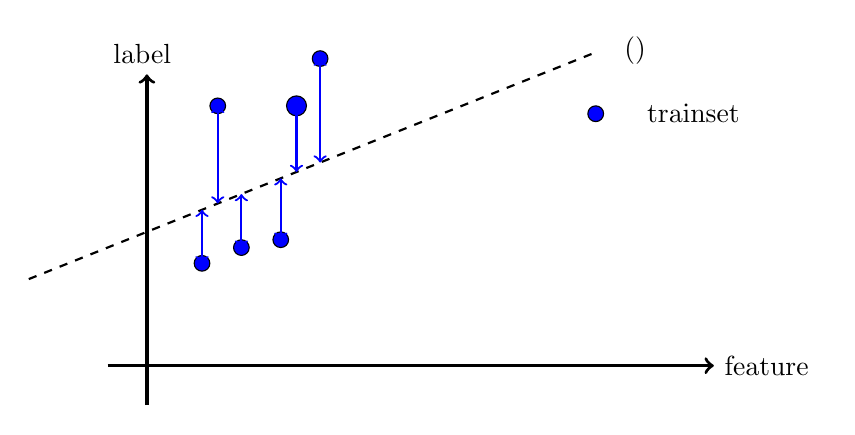
\begin{tikzpicture}[scale = 1]
					% Axes
					\draw[->, very thick] (0,0.5) -- (7.7,0.5) node[right] {\gls{feature} $\feature$};       % X-axis
					\draw[->, very thick] (0.5,0) -- (0.5,4.2) node[above] {\gls{label} $\truelabel$};   % Y-axis
					\draw[color=black, thick, dashed, domain = -1: 6.2, variable = \x]  plot ({\x},{\x*0.4 + 2.0}) ;      
					% Add a lasso around the two dashed lines
	          			% Ellipse around the two dashed lines
					\node at (6.7,4.5) {$\hypothesis(\feature)$};    
					\coordinate (l1)   at (1.2, 1.2*0.4+2.0);
					\coordinate (l2) at (1.4, 1.4*0.4+2.0);
					\coordinate (l3)   at (1.7, 1.7*0.4+2.0);
					\coordinate (l4)   at (2.2, 2.2*0.4+2.0);
					\coordinate (l5) at (2.4, 2.4*0.4+2.0);
					\coordinate (l6)   at (2.7,  2.7*0.4+2.0);
					\coordinate (n1)   at (1.2, 1.8);
					\coordinate (n2) at (1.4, 3.8);
					\coordinate (n3)   at (1.7,  2.0);
					\coordinate (n4)   at (2.2, 2.1);
					\coordinate (n5) at (2.4, 3.8);
					\coordinate (n6)   at (2.7,  4.4);
					\node at (n1)  [circle,draw,fill=blue,minimum size=6pt, scale=0.6]{};
					\node at (n3)  [circle,draw,fill=blue,minimum size=6pt, scale=0.6]{};
					\node at (n4)  [circle,draw,fill=blue,minimum size=6pt, scale=0.6]{};
					\node at (n2)  [circle,draw,fill=blue,minimum size=6pt, scale=0.6, name=c2] {};
					\node at (n5)  [circle,draw,fill=blue,minimum size=12pt,scale=0.6,  name=c5] {};
					\node at (n6)  [circle,draw,fill=blue,minimum size=6pt, scale=0.6]{};
					\draw[<->, color=blue, thick] (l1) -- (n1);  
					\draw[<->, color=blue, thick] (l2) -- (n2);  
					\draw[<->, color=blue, thick] (l3) -- (n3);  
					\draw[<->, color=blue, thick] (l4) -- (n4);  
					\draw[<->, color=blue, thick] (l5) -- (n5);  
					\draw[<->, color=blue, thick] (l6) -- (n6);  
					\draw[fill=blue] (6.2, 3.7)  circle (0.1cm) node [black,xshift=1.3cm] {\gls{trainset} $\dataset$};
				\end{tikzpicture}
				\caption{ERM aprende una hipótesis $\hypothesis\in \hypospace$, a partir de un modelo $\hypospace$, 
				minimizando la perdida promedio (o riesgo empírico) $\frac{1}{\samplesize} \sum\limits_{\sampleidx=1}^\samplesize \lossfunc{\pair{\featurevec^{(\sampleidx)}}{ \truelabel^{(\sampleidx)}}}{\hypothesis}$ 
				incurrida en un conjunto de entrenamiento $\dataset$. \label{fig_erm_dict} }
			\end{center}
		\end{figure} 
		La Figura \ref{fig_erm_dict} ilustra ERM para un modelo lineal y puntos de datos 
		que se caracterizan por un único atributo $\feature$ y una etiqueta $\truelabel$. 
		La hipótesis $\hypothesis$ es un mapa lineal que predice la etiqueta de un punto de datos
		como una función lineal de su atributo $\feature$, es decir, 
		$\hypothesis(\feature) = \weight_{1} \feature + \weight_{0}$, donde $\weight_{1}$ y $\weight_{0}$ son los 
		parametros del modelo de la hipótesis $\hypothesis$. El problema de ERM consiste en encontrar los 
		parametros del modelo $\weight_{1}$ y $\weight_{0}$ que minimicen la perdida promedio 
		incurrida por la hipótesis $\hypothesis$ en el conjunto de entrenamiento $\dataset$.	
		Vea también: \Gls{emprisk}, \gls{hypothesis}, \gls{model}, \gls{minimum}, \gls{loss}, gls{emprisk}, \gls{dataset}, \gls{trainset}, \gls{ml} },
	first={minimización empírica del riesgo (ERM)},text={ERM} }

\newglossaryentry{multilabelclass}{name={clasificación multi-etiqueta}, description={Los problemas y métodos de  
		clasificación multi-etiqueta\index{multi-label classification} utilizan puntos de datos
		caracterizados por varias etiquetas. Por ejemplo, considere un punto de datos
		que representa una imagen con dos etiquetas. Una etiqueta indica la presencia de un ser humano 
		en la imagen y otra etiqueta indica la presencia de un aútomovil.
		\\
		Vea también: \gls{classification}, \gls{datapoint}, \gls{label}},
	    first={clasificación multi-etiqueta},text={clasificación multi-etiqueta} }


\newglossaryentry{ssl}{name={aprendizaje semi-supervisado (SSL)}, description={El aprendizaje semi-supervisado (SSL)\index{aprendizaje semi-supervisado (SSL)} 
		utiliza puntos de datos no etiquetados para apoyar el aprendizaje de una hipótesis 
		a partir de puntos de datos etiquetados \cite{SemiSupervisedBook}. Este enfoque es particularmente útil 
		para aplicaciones de aprendizaje automático que ofrecen una gran cantidad de puntos de datos no etiquetados, pero solo un número limitado
		de puntos de datos etiquetados.
		\\
		Vea también: \gls{datapoint}, \gls{hypothesis}, \gls{labeled datapoint}, \gls{ml}, \gls{datapoint}  }, 
		first={aprendizaje semi-supervisado (SSL)},text={SSL} }
	
	
		\newglossaryentry{objfunc}{
			name={función objetivo},
			description={Una\index{función objetivo} función objetivo es un mapa que asigna un valor numérico 
			objetivo $f(\weights)$ a cada elección $\weights$ de una variable que deseamos 
			optimizar (véa Fig. \ref{fig_obj_func_dict}). En el contexto del aprendizaje automático, la variable de optimización 
			puede ser el conjunto de parametros del modelo de una hipótesis $\hypothesis^{(\weights)}$. 
			Entre las funciones objetivo comunes se encuentran el riesgo (es decir, la perdida esperada) 
			y el riesgo empírico (es decir, la perdida promedio sobre el conjunto de entrenamiento). Los métodos de aprendizaje automático
			aplican técnicas de optimización, como los metodos por gradiente, para encontrar la elección 
			$\weights$ que produzca el valor óptimo (por ejemplo, el minimo o el maximo) 
			de la función objetivo.
			\\
			\begin{figure}[H]
				\begin{center}
				\begin{tikzpicture}[scale=1.0]
					% Ejes
					\draw[->] (-0.5,0) -- (4.5,0) node[right] {$\weights$};
					\draw[->] (0,-0.5) -- (0,3.5);
					% Curva de la función objetivo
					\draw[thick,domain=0.3:4,smooth,variable=\x] 
					plot ({\x}, {0.5*(\x-2)^2 + 0.5});
					% Etiqueta de la curva
					\node at (3.5,2.8) {$f(\weights)$};
				\end{tikzpicture} 
				\end{center}
			\caption{Una función objetivo asigna a cada valor posible $\weights$ de una variable de optimización, 
			como los parametros del modelo de un modelo de aprendizaje automático, un valor que mide la utilidad 
			de $\weights$.\label{fig_obj_func_dict}}
			\end{figure} 
			Véa también: \gls{function}, \gls{map}, \gls{ml}, \glspl{modelparam}, \gls{hypothesis}, \gls{risk}, \gls{loss}, \gls{emprisk}, \gls{trainset}, \gls{gdmethods}, \gls{minimum}, \gls{maximum}, \gls{model}, \gls{lossfunc}.},
			first={función objetivo},
			text={función objetivo}
			}
			
\newglossaryentry{regularizer}{name={regularizador}, description={Un regularizador\index{regularizador} 
		asigna a cada hipótesis $\hypothesis$ de un espacio de hipótesis $\hypospace$ una medida cuantitativa 
		$\regularizer{\hypothesis}$ que indica cuánto podría diferir su error de prediccion en un conjunto de entrenamiento de 
		sus errores de predicción en puntos de datos fuera del conjnto de entrenamiento. La regresión ridge
		utiliza el regularizador $\regularizer{\hypothesis} \defeq \normgeneric{\weights}{2}^{2}$ para mapas de hipótesis lineales $\hypothesis^{(\weights)}(\featurevec) \defeq \weights^{T} \featurevec$ \cite[Ch. 3]{MLBasics}. 
		El operador de reducción y selección absoluta mínima (Lasso) utiliza el regularizador $\regularizer{\hypothesis} \defeq \normgeneric{\weights}{1}$ 
		para mapas de hipótesis lineales $\hypothesis^{(\weights)}(\featurevec) \defeq \weights^{T} \featurevec$ \cite[Ch. 3]{MLBasics}. 
		\\
		Vea también: \gls{hypothesis}, \gls{hypospace}, \gls{prediction}, \gls{trainset}, \gls{datapoint}, \gls{trainset}, \Gls{ridgeregression}, \Gls{lasso} },first={regularizador},text={regularizador} }


		\newglossaryentry{regularization}{name={regularización}, description={
			Un desafío clave de las aplicaciones modernas de aprendizaje automático es que a menudo 
			usan modelos grandes, que tienen un dimension efectiva del orden de miles de millones. 
			Entrenar un modelo de alta dimensión utilizando métodos basados en ERM
			es propenso al sobreajuste, es decir, la hipótesis aprendida tiene un buen 
			rendimiento en el conjunto de entrenamiento pero un rendimiento pobre fuera del conjunto de entrenamiento. 
			La regularización se refiere a modificaciones de una instancia dada de ERM 
			para evitar el sobreajuste, es decir, para asegurar que la hipótesis aprendida 
			no tenga un rendimiento mucho peor fuera del conjunto de entrenamiento. Existen tres rutas para implementar 
			la regularización: 
			\begin{enumerate}[label=\arabic*)]
				\item {Modelo podado:} Podamos el modelo original $\hypospace$ para obtener un 
				modelo más pequeño $\hypospace'$. Para un modelo paramétrico, el podado puede 
				implementarse mediante restricciones en los parametros del modelo (como $w_{1} \in [0.4,0.6]$ para 
				el peso del atributo $x_{1}$ en regresin lineal).
				\item {Perdida penalización:} Modificamos la funcion objetivo de ERM añadiendo un 
				término de penalización al error de entrenamiento. El término de penalización estima cuánto mayor es 
				la perdida esperada (o riesgo) en comparación con la perdida promedio en el conjunto de entrenamiento. 
				\item {Aumentación de Datos:} Podemos ampliar el conjunto de entrenamiento $\dataset$ añadiendo 
				copias perturbadas de los puntos de datos originales en $\dataset$. Un ejemplo de tal 
				perturbación es añadir la realización de una variable aleatoria al vector de atributos 
				de un punto de datos. 
			\end{enumerate} 
			La Fig. \ref{fig_equiv_dataaug_penal_dict} ilustra las tres rutas anteriores para la regularización. 
			Estas rutas están estrechamente relacionadas y, a veces, son completamente equivalentes. La aumentación de datos usando variables aleatorias gaussianas 
			para perturbar los vectores de atributos en el conjunto de entrenamiento de regresion lineal
			tiene el mismo efecto que añadir la penalización 
			$\lambda \normgeneric{\weights}{2}^2$ al error de entrenamiento (que no es más que regresión ridge). 
			La decisión sobre qué ruta usar para la regularización puede basarse en la 
			infraestructura computacional disponible. Por ejemplo, podría ser mucho más fácil 
			implementar aumentación de datos que el podado de modelo. 
			\begin{figure}[H]
				\begin{center} 
					\begin{tikzpicture}[scale = 1]
						% Axes
						\draw[->, very thick] (0,0.5) -- (7.7,0.5) node[right] {atributo $\feature$};       % X-axis
						\draw[->, very thick] (0.5,0) -- (0.5,4.2) node[above] {etiqueta $\truelabel$};   % Y-axis
						\draw[color=black, thick, dashed, domain = -1: 6.2, variable = \x]  plot ({\x},{\x*0.4 + 2.0}) ;     
						\draw[color=black, thick, dashed, domain = -1: 6.2, variable = \x]  plot ({\x},{\x*0.6 + 2.0}) ;     
									% Add a lasso around the two dashed lines
				  % Ellipse around the two dashed lines
						\draw[blue, thick] (5, 4.5) ellipse [x radius=0.2cm, y radius=1cm];
						\node at (5, 5.8) [text=black, font=\small] {$\{ \hypothesis: \hypothesis(x)\!=\!w_{1}x\!+\!w_{0}; w_{1} \in [0.4,0.6]\}$};
						\node at (6.7,4.5) {$\hypothesis(\feature)$};    
						\coordinate (l1)   at (1.2, 2.48);
						\coordinate (l2) at (1.4, 2.56);
						\coordinate (l3)   at (1.7,  2.68);
						\coordinate (l4)   at (2.2, 2.2*0.4+2.0);
						\coordinate (l5) at (2.4, 2.4*0.4+2.0);
						\coordinate (l6)   at (2.7,  2.7*0.4+2.0);
						\coordinate (l7)   at (3.9,  3.9*0.4+2.0);
						\coordinate (l8) at (4.2, 4.2*0.4+2.0);
						\coordinate (l9)   at (4.5,  4.5*0.4+2.0);
						\coordinate (n1)   at (1.2, 1.8);
						\coordinate (n2) at (1.4, 1.8);
						\coordinate (n3)   at (1.7,  1.8);
						\coordinate (n4)   at (2.2, 3.8);
						\coordinate (n5) at (2.4, 3.8);
						\coordinate (n6)   at (2.7,  3.8);
						% augemented data point obtained by perturbing feature, not touching label value 
						\coordinate (n7)   at (3.9, 2.6);
						\coordinate (n8) at (4.2, 2.6);
						\coordinate (n9)   at (4.5,  2.6);
						\node at (n1)  [circle,draw,fill=red,minimum size=6pt,scale=0.6, name=c1] {};
						\node at (n2)  [circle,draw,fill=blue,minimum size=6pt, scale=0.6, name=c2] {};
						\node at (n3)  [circle,draw,fill=red,minimum size=6pt,scale=0.6,  name=c3] {};
						\node at (n4)  [circle,draw,fill=red,minimum size=12pt, scale=0.6, name=c4] {};  
						\node at (n5)  [circle,draw,fill=blue,minimum size=12pt,scale=0.6,  name=c5] {};
						\node at (n6)  [circle,draw,fill=red,minimum size=12pt, scale=0.6, name=c6] {};  
						\node at (n7)  [circle,draw,fill=red,minimum size=12pt,scale=0.6,  name=c7] {};
						\node at (n8)  [circle,draw,fill=blue,minimum size=12pt, scale=0.6, name=c8] {};
						\node at (n9)  [circle,draw,fill=red,minimum size=12pt, scale=0.6, name=c9] {};
						\draw [<->] ($ (n7) + (0,-0.3) $)  --  ($ (n9) + (0,-0.3) $) node [pos=0.4, below] {$\sqrt{\regparam}$}; ; 
						\draw[<->, color=red, thick] (l1) -- (c1);  
						\draw[<->, color=blue, thick] (l2) -- (c2);  
						\draw[<->, color=red, thick] (l3) -- (c3);  
						\draw[<->, color=red, thick] (l4) -- (c4);  
						\draw[<->, color=blue, thick] (l5) -- (c5);  
						\draw[<->, color=red, thick] (l6) -- (c6);  
						\draw[<->, color=red, thick] (l7) -- (c7);  
						\draw[<->, color=blue, thick] (l8) -- (c8);  
						\draw[<->, color=red, thick] (l9) -- (c9);  
						\draw[fill=blue] (6.2, 3.7)  circle (0.1cm) node [black,xshift=2.3cm] {conjunto de entrenamiento $\dataset$};
						\draw[fill=red] (6.2, 3.2)  circle (0.1cm) node [black,xshift=1.3cm] {ampliado};
						\node at (4.6,1.2)  [minimum size=12pt, font=\fontsize{12}{0}\selectfont, text=blue] {$\frac{1}{\samplesize} \sum_{\sampleidx=1}^\samplesize \lossfunc{\pair{\featurevec^{(\sampleidx)}}{ \truelabel^{(\sampleidx)}}}{\hypothesis}$};
						\node at (7.8,1.2)  [minimum size=12pt, font=\fontsize{12}{0}\selectfont, text=red] {$+\regparam \regularizer{\hypothesis}$};
					\end{tikzpicture}
					\caption{Tres enfoques para la regularización: 1) Aumentación de datos; 2) penalización de perdida; y 3) modelo
					podado (mediante restricciones en parametros del modelo). \label{fig_equiv_dataaug_penal_dict} }
				\end{center}
			\end{figure} 
			Véa también: \gls{ml}, \gls{model}, \gls{effdim}, \gls{erm}, \gls{overfitting}, \gls{hypothesis}, \gls{trainset}, \glspl{modelparam}, \gls{feature}, \gls{linreg}, \gls{loss}, \gls{objfunc}, \gls{trainerr}, \gls{risk}, \gls{dataaug}, \gls{datapoint}, \gls{realization}, \gls{rv}, \gls{featurevec}, \gls{gaussrv}, \gls{ridgeregression}, \gls{label}.
			},first={regularización},text={regularización} }

\newglossaryentry{rerm}{
	name={minimización del riesgo empírico regularizado (RERM)}, 
	description={El ERM básico aprende una hipótesis (o entrena un modelo) $\hypothesis \in \hypospace$ 
		basado únicamente en el riesgo empírico $\emprisk{\hypothesis}{\dataset}$ incurrido en un conjunto de entrenamiento $\dataset$. 
		Para hacer que ERM sea menos propenso al sobreajuste, podemos implementar la regulación 
		incluyendo un regularizador (escalado) $\regularizer{\hypothesis}$ en el objetivo de aprendizaje. 
		Esto da lugar a la minimización del riesgo empírico regularizado (RERM)\index{minimización del riesgo empírico regularizado (RERM)}, 
		\begin{equation}
			\label{equ_def_rerm}
			\learnthypothesis \in \argmin_{\hypothesis \in \hypospace} \emprisk{\hypothesis}{\dataset} + \regparam \regularizer{\hypothesis}.
		\end{equation}
		El parámetro $\regparam \geq 0$ controla la intensidad de la regulación. 
		Para $\regparam = 0$,  recuperamos el ERM estándar sin regulación. A medida que $\regparam$ aumenta, la 
		hipótesis aprendida se inclina cada vez más hacia valores pequeños de $\regularizer{\hypothesis}$. 
		El componente $\regparam \regularizer{\hypothesis}$ en la funcion objetivo de \eqref{equ_def_rerm} 
		se puede entender intuitivamente como un sustituto para el aumento promedio en la perdida que puede 
		ocurrir al predecir etiquetas para puntos de datos fuera del conjunto de entrenamiento. Esta intuición  
		se puede precisar en varias maneras. Por ejemplo, considere un modelo lineal entrenado usando pérdida de error cuadrático
		y el regularizador $\regularizer{\hypothesis} = \normgeneric{\weights}{2}^{2}$. 
		En este caso, $\regparam \regularizer{\hypothesis}$ corresponde al aumento esperado en la perdida 
		causado por la adición de variables aleatorias gaussianas a los vectores de atributos en el conjunto de entrenamiento
		\cite[Ch. 3]{MLBasics}.
		Una construcción basada en principios para el regularizador $\regularizer{\hypothesis}$ 
		surge de límites superiores aproximados en el error de generalización. La instancia resultante  
		de RERM se conoce como minimización del riesgo estructural (SRM) \cite[Sec. 7.2]{ShalevShwartz2009}.
		\\
		Vea también: \gls{erm},  \gls{hypothesis}, \gls{model}, \gls{emprisk}, \gls{trainset}, \gls{overfitting}, \gls{regularization}, \gls{regularizer}, \gls{datapoint}, \gls{loss}, \gls{label}, \gls{linmodel}, \gls{featurevec},   }, 
	first={minimización del riesgo empírico regularizado (RERM)},
	text={RERM} 
}


\newglossaryentry{generalization}{name={generalización}, 
	description={Muchos\index{generalización} de los sistemas actuales de aprenizaje automático (y inteligencia artificial)  
		se basan en ERM: En esencia, entrenan un modelo (es decir, aprenden una hipótesis
		$\learnthypothesis \in \hypospace$) minimizando la perdida promedia (o riesgo empírico) en algunos 
		putnos de datos $\vz^{(1)},\ldots,\vz^{(\samplesize)}$, que sirven como un conjunto de entrenamiento $\trainset$. 
		La generalización se refiere a la capacidad de un método de aprendizaje automático para desempeñarse bien fuera del conjunto de entrenamiento. 
		Cualquier teoría matemática de la generalización necesita algún concepto matemático para el  
		"fuera del conjunto de entrenamiento." Por ejemplo, la teoría del aprendizaje estadístico utiliza un  
		modelo de probabilidad como la suposición iid para la generacion de datos: los puntos de datos en 
		el conjunto de entrenamiento son realizaciónes iid de alguna distribución de probabilidad subyacente $p(\vz)$. 
		Un modelo de probabilidad nos permite explorar el exterior del conjunto de entrenamiento generando 
		adicionales realizaciónes iid de $p(\vz)$. Además, el uso de la suposición i.i.d
		nos permite definir el riesgo de un modelo entrenado $\learnthypothesis \in \hypospace$ como 
		la expectativa de la perdida $\risk{\learnthypothesis}$. Además, podemos utilizar límites de concentración  
		o resultados de convergencia para secuencias de variables aleatorias iid para limitar la desviación  
		entre el riesgo empírico $\emprisk{\learnthypothesis}{\trainset}$ de un modelo entrenado y 
		su riesgo \cite{ShalevMLBook}. También es posible estudiar la generalización sin utilizar 
		modelos de probabilidad. Por ejemplo, podríamos utilizar perturbaciones (determinísticas)  
	    de los puntos de datos en el conjunto de entrenamiento para estudiar su exterior. 
	    En general, deseamos que el modelo entrenado sea robusto, es decir, que sus predicciónes 
	    no cambien demasiado ante pequeñas perturbaciones de un punto de datos. Considere un modelo entrenado para detectar 
	    un objeto en una imagen capturada por un teléfono inteligente. El resultado de la detección no debería cambiar si 
	    enmascaramos un pequeño número de píxeles seleccionados aleatoriamente en la imagen \cite{OnePixelAttack}. 
		  \begin{figure}[H]
		                   	\centering
		                   	\begin{tikzpicture}[scale=0.8]
 % Filled ellipsoid to represent p(z)
							   \draw[lightblue, fill=lightblue, opacity=0.5] (3, 2) ellipse (6cm and 2cm);
% Label for p(z)
								\node[black] at (6, 3) {$p(z)$};
		                   		% Data points
		                   		\fill[blue] (1, 3) circle (4pt) node[below, xshift=0pt, yshift=0pt] {$\datapoint^{(1)}$};
		                   		\fill[blue] (5, 1) circle (4pt) node[below] {$\datapoint^{(2)}$};
		                   		% Shifted copies for datapoint^{(1)}
		                   		\fill[blue] (1.6, 3) circle (3pt);
		                   		\fill[blue] (0.4, 3) circle (3pt);
		                   		\draw[<->, thin] (1, 3) -- (1.6, 3);
		                   		\draw[<->, thin] (1, 3) -- (0.4, 3);
		                   		% Shifted copies for datapoint^{(2)}
		                   		\fill[blue] (5.6, 1) circle (3pt);
		                   		\fill[blue] (4.4, 1) circle (3pt);
		                   		\draw[<->, thin] (5, 1) -- (5.6, 1);
		                   		\draw[<->, thin] (5, 1) -- (4.4, 1);
		                   		% Polynomial curve
		                   		\draw[black, thick, domain=0:6, smooth] plot (\x, {- 1*\x + 5});
		                   		% Label for polynomial
		                   		\node[black] at (3, 2.5) [right] {$\learnthypothesis$};
		                   	\end{tikzpicture}
		                   	\caption{Dos puntos de datos $\datapoint^{(1)},\datapoint^{(2)}$ que se utilizan como un conjunto de entrenamiento
							   	para aprender una hipótesis $\learnthypothesis$ mediante ERM. Podemos evaluar $\learnthypothesis$ 
		                   		fuera de $\trainset$ ya sea mediante una suposición iid con alguna distribución de probabilidad subyacente $p(\datapoint)$ 
		                   		o mediante la perturbación de los puntos de datos.}
		                   	\label{fig:polynomial_fit_dict}
		                   \end{figure}
		                   \newpage
		},
	first={generalización},text={generalización} }

	\newglossaryentry{gengap}
{name = {brecha de generalización}, 
	description={La diferencia\index{brecha de generalización} entre el rendimiento de un modelo
		entrenado sobre el conjunto de entrenamiento y su rendimiento sobre otros puntos de datos
		(como los del conjunto de validacion).\\
		Véa también: \gls{model}, \gls{trainset}, \gls{datapoint}, \gls{valset}, \gls{hypothesis}, 
		\gls{decisiontree}, \gls{generalization}, \gls{gdmethods}, \gls{erm}, \gls{smooth}, 
		\gls{lossfunc}, \gls{gd}, \glspl{modelparam}, \gls{emprisk}, \gls{gradient}, \gls{loss}, 
		\gls{gradstep}.
	}, 
	first={brecha de generalización}, 
	text={brecha de generalización}
}

		
		\newglossaryentry{concentrationinequ}
		{name = {desigualdad de concentración}, 
			description={Una cota superior para la \gls{probability}\index{desigualdad de concentración} 
				de que una \gls{rv} se desvíe más de una cantidad prescrita respecto a su \gls{expectation} \cite{Wain2019}.\\
				Véa también: \gls{probability}, \gls{rv}, \gls{expectation}.
			}, 
			first={desigualdad de concentración},  
			text={desigualdad de concentración}
		}
		

	\newglossaryentry{boosting}
	{name = {boosting}, 
		description={El boosting\index{boosting} es un metodo de optimización iterativo para aprender una 
		función de hipótesis precisa (o strong learner) combinando secuencialmente 
		funciones de hipótesis menos precisas (conocidas como weak learners) \cite[Cap. 10]{hastie01statisticallearning}. 
		Por ejemplo, los weak learners suelen ser árboles de decisión poco profundos que se combinan 
		para obtener un árbol de decisión profundo. El boosting puede entenderse como una 
		generalización de los metodos de descenso por gradiente para ERM utilizando modelos paramétricos 
		y funciones de perdida suaves \cite{Friedman2001}. Así como el descenso por gradiente actualiza iterativamente 
		los parametros del modelo para reducir el rieso empírico, el boosting combina iterativamente 
		(ej., por suma) funciones de hipótesis para reducir dicho riesgo empírico. 
		Una variante ampliamente utilizada del enfoque general de boosting es el boosting gradiente, 
		que emplea el gradiente de la función de perdida para combinar los weak learners \cite{Friedman2001}.
		\begin{figure}[H]
			\begin{center}
				\begin{tikzpicture}[scale=1.2]
					% Axes
					\draw[->] (-0.5,0) -- (5.5,0) node[right] {$\hypothesis$};
					\draw[->] (0,-0.5) -- (0,4.5) node[above] {$\lossfunc{\vz}{\hypothesis}$};
					\draw[thick,domain=0.2:5,smooth,variable=\x,blue!60] plot ({\x},{(4 - 1.3*\x + 0.15*\x*\x)});
					\foreach \x/\label in {0.7/$\hypothesis^{(0)}$, 1.5/$\hypothesis^{(1)}$, 2.3/$\hypothesis^{(2)}$, 3.0/$\hypothesis^{(3)}$} {
						\draw[dashed, gray] (\x, 0) -- (\x, {4 - 1.3*\x + 0.15*\x*\x}); % helper line
						\filldraw[black] (\x, {4 - 1.3*\x + 0.15*\x*\x}) circle (2pt);   % point
						\node[below] at (\x, -0.1) {\label};                             % label
					}
				\end{tikzpicture}
			\end{center} 
			\caption{Los métodos de boosting construyen una secuencia de funciones de hipótesis
			$\hypothesis^{(0)},\hypothesis^{(1)},\ldots$ que son cada vez mejores (es decir, incurren en menor perdida).}
		\end{figure}
		Véa también: \gls{hypothesis}, \gls{map}, \gls{decisiontree}, \gls{generalization}, \gls{gdmethods}, 
		\gls{erm}, \gls{model}, \gls{smooth}, \gls{lossfunc}, \gls{gd}, \glspl{modelparam}, \gls{emprisk}, 
		\gls{gradient}, \gls{loss}, \gls{gradstep}.
		}, 
		first={boosting}, 
		text={boosting}} 
	
	
\newglossaryentry{gtv}{name={variación total generalizada (GTV)}, description={GTV es una\index{variación total generalizada (GTV)} 
		medida de la variación de los modelos locales entrenados $\localhypothesis{\nodeidx}$ 
		(o de sus parametros del modelo $\localparams{\nodeidx}$) asignados a los nodos $\nodeidx=1,\ldots,\nrnodes$ 
		de un grafo no dirigido ponderado $\graph$ con aristas $\edges$. Dada una medida $\discrepancy{\hypothesis}{\hypothesis'}$ 
		para la discrepancia entre mapas de hipótesis $\hypothesis,\hypothesis'$, la GTV se define como:
		\begin{equation} 
			\nonumber
			\sum_{\edge{\nodeidx}{\nodeidx'}\in \edges} \edgeweight_{\nodeidx,\nodeidx'} 
			\discrepancy{\localhypothesis{\nodeidx}}{\localhypothesis{\nodeidx'}}.
		\end{equation}
		Here, $\edgeweight_{\nodeidx,\nodeidx'}>0$ denota el peso de la arista no dirigida $\edge{\nodeidx}{\nodeidx'}\in \edges$.
		\\
		Vea también: \gls{localmodel}, \glspl{modelparam}, \gls{graph}, \gls{discrepancy}, \gls{hypothesis} },first={GTV},text={GTV} }
	
\newglossaryentry{srm}{
	name={minimización del riesgo estructural (SRM)},
	description={La minimización del riesgo estructural (SRM)\index{minimización del riesgo estructural (SRM)} es una
		forma de minimización del riesgo empírico regularizado (RERM), en la que el modelo $\hypospace$ se puede expresar 
		como una unión contable de submodelos: $\hypospace = \bigcup_{n=1}^{\infty} \hypospace^{(n)}$. 
		Cada submodelo $\hypospace^{(n)}$ permite la derivación de un límite superior aproximado 
		para el error de generalización que se incurre al aplicar ERM para entrenar $\hypospace^{(n)}$. 
		Estos límites superiores individuales para cada submodelo—se combinan para formar un regularizador
		utilizado en el objetivo de RERM.  
        Estos límites superiores aproximados (uno para cada $\hypospace^{(n)}$) se combinan 
		para construir un regularizador para RERM \cite[Sec.\ 7.2]{ShalevMLBook}.
		\\
		Vea también: \gls{rerm}, \gls{model}, \gls{erm}, \gls{regularizer}   },
		text={SRM}
 }
 
 \newglossaryentry{rlm}{
 	name={minimización de la pérdida regularizada (RLM)},
 	description={Consulte\index{minimización de la pérdida regularizada (RLM)} \gls{rerm}.},
 	text={RLM}
 }
 
 \newglossaryentry{datapoisoning}{
	name={envenenamiento de datos},
	description={El \index{envenenamiento de datos} envenenamiento de datos se refiere a la manipulación 
	(o fabricación) intencionada de puntos de datos con el fin de influir en el entrenamiento de un modelo 
	de aprendizaje automático \cite{Liu2021}, \cite{PoisonGAN}. 
	Los ataques de envenenamiento de datos pueden adoptar diversas formas, entre las cuales se incluyen:
	\begin{itemize}
		\item Puerta trasera: Consiste en implantar disparadores (triggers) en los datos de entrenamiento, 
		de manera que el modelo entrenado se comporte normalmente con vectores de atributos típicos, 
		pero clasifique erróneamente un vector de atributos que contiene un patrón de disparo.
		\item Ataque de denegación de servicio(DDoS): Buscan degradar el rendimiento general del modelo entrenado mediante la inyección 
		de ejemplos mal etiquetados o adversarios para impedir un aprendizaje efectivo.
	\end{itemize}
	El envenenamiento de datos es especialmente preocupante en entornos de aprendizaje automático descentralizados o distribuidos 
	(como en aprendizaje federado), donde no es posible verificar centralmente los datos de entrenamiento.
	\\
	Véa también: \gls{attack}, \gls{backdoor}, \gls{dosattack}, \gls{trustAI}.},
	first={envenenamiento de datos},
	text={envenenamiento de datos}
	}
	
	
\newglossaryentry{backdoor}{name={puerta trasera (backdoor)}, description={Un ataque de puerta trasera (backdoor)\index{puerta trasera (backdoor)} se refiere
		a la manipulación intencional del proceso de entrenamiento de un método de aprendizaje automático. Esta manipulación se puede
		implementar perturbando el conjunto de entrenamiento (envenenamiento de datos) o el
		algoritmo de optimización utilizado por un método basado en ERM. El objetivo 
		de un ataque de puerta trasera es inclinar la hipótesis aprendida $\learnthypothesis$ 
		hacia predicciones específicas para un rango determinado de valores de atributos. Este rango de atributos
		actúa como una clave (o desencadenante) que desbloquea una puerta trasera en el sentido de generar
		predicciones anómalas. La clave $\featurevec$ y la
		predicción anómala correspondiente $\learnthypothesis(\featurevec)$ son conocidas únicamente por el atacante.
		\\
		Vea también: \gls{ml}, \gls{trainset}, \gls{data}, \gls{algorithm}, \gls{erm}, \gls{hypothesis}, \gls{prediction}, \gls{feature},  },
	first={puerta trasera (backdoor)},text={backdoor} }


\newglossaryentry{clustasspt}{name={suposición de agrupamiento}, description={La suposición de agrupamiento\index{suposición de agrupamiento} 
		postula que los puntos de datos en un conjunto de datos forman un (pequeño) número de grupos o clústers.
		Los puntos de datos en el mismo clúster son más similares entre sí que aquellos
		que están fuera del clúster \cite{SemiSupervisedBook}. Obtenemos diferentes 
		métodos de agrupamiento utilizando diferentes nociones de similitud entre puntos de datos.
		\\
		Vea también:\gls{datapoint}, \gls{dataset}, \gls{cluster}, \gls{clustering} },first={suposición de agrupamiento},text={suposición de agrupamiento} }
	
\newglossaryentry{dosattack}{name={ataque de denegación de servicio (DoS)}, description={Un ataque de denegación de servicio (DoS)\index{ataque de denegación de servicio (DoS)} 
		tiene como objetivo (por ejemplo, mediante envenenamiento de datos) dirigir el entrenamiento de un modelo
		para que tenga un rendimiento deficiente con puntos de datos típicos.
		\\
		Vea también: \gls{datapoisoning}, \gls{model}, \gls{datapoint}},
	first={ataque de denegación de servicio (DoS)},text={ataque de denegación de servicio} }

\newglossaryentry{netexpfam}{name={familias exponenciales en red (nExpFam)}, 
	description={Una\index{familias exponenciales en red (nExpFam)} colección de familias exponenciales, 
		cada una de ellas asignada a un nodo de un red de aprendizaje federado (red FL). Los parametros del modelo están acoplados 
		a través de la estructura de la red al requerir que tengan una pequeña variación total generalizada (GTV) \cite{JungNetExp2020}.
		\\
		Vea también: \gls{empgraph}, \gls{gtv}},first={familia exponencial en red (nExpFam)},text={nExpFam} }
	 


\newglossaryentry{scatterplot}{name={diagrama de dispersión}, description={Un\index{diagrama de dispersión} 
		método de visualización que representa puntos de datos mediante marcadores en un plano bidimensional. 
		La Figura \ref{fig_scatterplot_temp_FMI_dict} depicta un ejemplo de un diagrama de dispersión.  
		\begin{figure}[H]
			\begin{center}
				\begin{tikzpicture}[scale=1]
					\tikzset{x=2cm,y=2cm,every path/.style={>=latex},node style/.style={circle,draw}}
					\begin{axis}[axis x line=none,
						axis y line=none,
						ylabel near ticks,
						xlabel near ticks,
						enlarge y limits=true,
						xmin=-5, xmax=30,
						ymin=-5, ymax=30,
						width=6cm, height=6cm ]
						\addplot[only marks] table [x=mintmp, y=maxtmp, col sep = semicolon] {../../assets/FMIData1.csv};
						\node at (axis cs:26,2) [anchor=west] {$\feature$};
						\node at (axis cs:0,30) [anchor=west] {$\truelabel$};
						\draw[->] (axis cs:-5,0) -- (axis cs:30,0);
						\draw[->] (axis cs:0,-5) -- (axis cs:0,30);
					\end{axis}
				\end{tikzpicture}
				\vspace*{-10mm}
			\end{center}
			\caption{Un diagrama de dispersión de algunos puntos de datos que representan las condiciones climáticas diarias en Finlandia. 
				Cada punto de datos se caracteriza por su temperatura minima diaria $\feature$ como 
				atributo y su temperatura máxima diaria $\truelabel$ como etiqueta. 
				Las temperaturas se han medido en la estación meteorológica FMI de Helsinki Kaisaniemi 
				durante el período 1.9.2024 - 28.10.2024.}
			\label{fig_scatterplot_temp_FMI_dict}
			\vspace*{-3mm}
			\end{figure}.
			\\
			Vea también: \gls{datapoint}, \gls{minimum}, \gls{feature}, \gls{maximum}, \gls{label}, \gls{fmi} },first={diagrama de dispersión},text={diagrama de dispersión} }


\newglossaryentry{stepsize}{name={tamaño de paso}, description={
		Consulte\index{tamaño de paso} \gls{learnrate}.}, 
	first={tamaño de paso},text={tamaño de paso} }

\newglossaryentry{learnrate}{name={tasa de aprendizaje}, description={Considere\index{tasa de aprendizaje} 
		un método iterativo de aprendizaje automático para encontrar o aprender una hipótesis útil $\hypothesis \in \hypospace$. 
		Dicho método iterativo repite pasos computacionales similares (de actualización) que ajustan o 
		modifican la hipótesis actual para obtener una hipótesis mejorada. Un 
		ejemplo bien conocido de este tipo de método de aprendizaje iterativo es el descenso por gradiente y sus variantes, descenso por gradiente estocástico y 
		descenso por gradiente proyectado. Un parámetro clave de un método iterativo es la tasa de aprendizaje. 
		La tasa de aprendizaje controla la magnitud en que la hipótesis actual
		puede modificarse durante una sola iteración. Un ejemplo conocido de este parámetro  
		es el tamaño de paso utilizado en descenso por gradiente \cite[Ch. 5]{MLBasics}.
		\\
		Vea también: \gls{ml}, \gls{hypothesis}, \gls{gd}, \gls{stochGD}, \gls{projgd}, \gls{stepsize}.},
	first={tasa de aprendizaje},text={tasa de aprendizaje} }

	\newglossaryentry{featuremap}
	{name={mapa de atributos}, 
		description={Un mapa de atributos\index{mapa de atributos} se refiere a una función
			$$
			\featuremapvec: \featurespace \rightarrow \featurespace', \quad \featurevec \mapsto \featurevec'
			$$
			que transforma un vector de atributos $\featurevec \in \featurespace$ de un punto de datos
			en un nuevo vector de atributos $\featurevec' \in \featurespace'$, donde típicamente 
			$\featurespace'$ es diferente de $\featurespace$.
			La representación transformada $\featurevec'$ suele ser más útil que la original $\featurevec$. 
			Por ejemplo, la geometría de los puntos de datos puede volverse más lineal en $\featurespace'$, 
			lo que permite aplicar un modelo lineal a $\featurevec'$. 
			Esta idea es central en el diseño de metodos de kernel~\cite{LearningKernelsBook}.
			Otros beneficios de usar un mapa de atributos incluyen la reducción del sobreajuste
			y la mejora de la interpretabilidad~\cite{Ribeiro2016}. Un caso de uso común es la visualización 
			de datos, donde un mapa de atributos con dos dimensiones de salida permite representar 
			punto de datos en un diagrama de dispersión 2D. Algunos métodos de aprendizaje automático emplean mapas de atributos
			entrenables, cuyos parametros se aprenden a partir de datos. Un ejemplo es el uso 
			de capas ocultas en una red profunda, que actúan como mapa de atributos sucesivos 
			\cite{MallatUnderstandingDeepLearning}. Una forma fundamentada de entrenar un mapa de atributos
			es mediante ERM, utilizando una funcion de perdida que mide la calidad de reconstrucción, 
			por ejemplo, $\lossfun = \|\featurevec - r(\featurevec')\|^2$, donde $r(\cdot)$ es un mapa 
			entrenable que intenta reconstruir $\featurevec$ a partir del vector de atributos transformado $\featurevec'$.
			\\
			Véa también: \gls{feature}, \gls{map}, \gls{kernelmethod}, \gls{featlearn}, \gls{pca}.},
		first={mapa de atributos},
		text={mapa de atributos} 
	}
	
	
 
  \newglossaryentry{lasso}{name={operador de reducción y selección absoluta mínima (Lasso)}, 
	description={El Lasso\index{loperador de reducción y selección absoluta mínima (Lasso)} es una
		implementación de minimización del riesgo estructural (SRM). Aprende los pesos $\weights$ de un mapa lineal 
		$\hypothesis(\featurevec) = \weights^{T} \featurevec$ basado en un conjunto de entrenamiento. 
		El Lasso se obtiene a partir de regresión lineal al agregar la norma $\ell_{1}$ escalado
		$\regparam \normgeneric{\weights}{1}$ al promedio de la pérdida de error cuadrático en el conjunto de entrenamiento. 
		\\
		Vea también: \gls{srm}, \gls{weights}, \gls{trainset}, \gls{linreg}, \gls{norm}, \gls{sqerrloss}.},
	first={Lasso},text={Lasso} }
 
 \newglossaryentry{simgraph}{name={grafo de similitud}, 
 	description={Algunas\index{grafo de similitud} aplicaciones de aprendizaje automático generan puntos de datos que 
	 	están relacionados por una noción de similitud específica del dominio. Estas similitudes pueden ser 
	 	representadas convenientemente utilizando un grafo de similitud $\graph = \big(\nodes \defeq \{1,\ldots,\samplesize\},\edges\big)$. 
 		El nodo $\sampleidx \in \nodes$ representa el $\sampleidx$-ésimo punto de datos. Dos 
 		nodos están conectados por una arista no dirigida si los puntos de datos correspondientes son similares.
		 \\
		 Vea también: \gls{ml}, \gls{datapoint}, \gls{graph}.},
 	first={grafo de similitud},text={grafo de similitud} }
 
 
 \newglossaryentry{kld}{name={divergencia de Kullback-Leibler (divergencia KL)}, 
 	description={
 		 La\index{divergencia de Kullback-Leibler (divergencia KL)} divergencia KL es una medida cuantitativa 
 		 de cuánto se diferencia una distribución de probabilidad de otra distribución de probabilidad \cite{coverthomas}.  
		  \\
		  Vea también: \gls{probdist}},
 	first={divergencia de Kullback-Leibler (divergencia KL)},text={divergencia KL} }

\newglossaryentry{LapMat}{
	name={matriz laplaciana},
	description={La\index{matriz laplaciana} estructura de un grafo $\graph$, con 
		nodos $\nodeidx=1,\ldots,\nrnodes$, se puede analizar utilizando las propiedades de 
		matrices especiales asociadas con $\graph$. Una de estas matrices es la
		matriz laplaciana del grafo $\mL^{(\graph)} \in \mathbb{R}^{\nrnodes \times \nrnodes}$, 
		la cual se define para un grafo no dirigido y ponderado \cite{Luxburg2007,Ng2001}. 
		Se define de forma elemento por elemento como (Vea la Figura \ref{fig_lap_mtx_dict})
	\begin{equation}
		\LapMatEntry{\graph}{\nodeidx}{\nodeidx'} \defeq \begin{cases} - \edgeweight_{\nodeidx,\nodeidx'} & \mbox{ para } \nodeidx\neq \nodeidx', \edge{\nodeidx}{\nodeidx'}\!\in\!\edges, \\ 
			\sum_{\nodeidx'' \neq \nodeidx} \edgeweight_{\nodeidx,\nodeidx''} & \mbox{ para } \nodeidx = \nodeidx', \\ 
							0 & \mbox{ en otro caso.} \end{cases}
	 \end{equation}
  Aqui, $\edgeweight_{\nodeidx,\nodeidx'}$ denota el peso de arista de una arista $\edge{\nodeidx}{\nodeidx'} \in \edges$. 
  \begin{figure}[H]
  	\begin{center}
    \begin{minipage}{0.45\textwidth}
	\begin{tikzpicture}
%	 				% 		% Left part - Graph
	 	 		\begin{scope}[every node/.style={circle, draw, minimum size=1cm}]
	 					 			\node (1) at (0,0) {1};
	 					 			\node (2) [below left=of 1] {2};
	 					 			\node (3) [below right=of 1] {3};
	 					 		   \draw (1) -- (2);
	 					 			\draw (1) -- (3);
	 					 		\end{scope}
	 				 	\end{tikzpicture}
	 			 	\end{minipage} 
	 			 	\hspace*{-15mm}
 		 		\begin{minipage}{0.45\textwidth}
	 			 	 \begin{equation} 
	 				 		 \LapMat{\graph} = \begin{pmatrix} 2 & -1& -1 \\ -1& 1 & 0 \\  -1 & 0 & 1 \end{pmatrix}  
	 				 		 \nonumber
	 				 		 \end{equation} 
	 			 \end{minipage}
	 	 \caption{\label{fig_lap_mtx_dict} Izquierda: Un grafo no dirigido $\graph$ con tres nodos $\nodeidx=1,2,3$. 
	 		 	Derecha: La matriz laplaciana $\LapMat{\graph}  \in \mathbb{R}^{3 \times 3}$ of $\graph$.} 
	 		 	\end{center}
	 		\end{figure}
	%		
	Vea también \gls{graph}, \gls{edgeweight}.},
	first={matriz laplaciana},
	text={matriz laplaciana}
}

\newglossaryentry{algconn}{
	name={conectividad algebraica},
	description={La\index{conectividad algebraica} conectividad algebraica de un grafo no dirigido 
		es el segundo valor propio más pequeño $\eigval{2}$ de su matriz laplaciana. 
		Un grafo es conexo si y solo si $\eigval{2} > 0$.\\
		Véa también: \gls{graph}, \gls{eigenvalue}, \gls{LapMat}.
	},
	first={conectividad algebraica},
	text={conectividad algebraica}
}


\newglossaryentry{cfwmaxmin}{name ={caracterización min-max de Courant–Fischer–Weyl}, 
description={Considere\index{caracterización min-max de Courant–Fischer–Weyl} una 
		matriz semi-definida positiva  $\mQ \in \mathbb{R}^{\nrfeatures \times \nrfeatures}$ con 
		descomposición en valores propios (o descomposición espectral), 
		$$ \mQ = \sum_{\featureidx=1}^{\nrfeatures} \eigval{\featureidx} \vu^{(\featureidx)} \big(  \vu^{(\featureidx)}  \big)^{T}.$$ 
		Aquí, utilizamos los valores propios ordenados (de forma creciente) 
		\begin{equation}
			\nonumber
			%	\label{equ_def_order_eigvals_LapMat}  
			 \eigval{1}  \leq  \ldots \leq \eigval{\nrnodes}. 
		\end{equation}
		La caracterización min-max de Courant–Fischer–Weyl \cite[Th. 8.1.2]{GolubVanLoanBook} 
		representa los valores propios de $\mQ$ como las soluciones a ciertos problemas de optimización.
		\\
		Vea también: \gls{psd}, \gls{evd}, \gls{eigenvalue}.}, 
	first = {caracterización min-max de Courant–Fischer–Weyl (CFW)}, 
	text={CFW}}

	\newglossaryentry{kernel}
	{name={kernel}, 
		description={Considere\index{kernel} un conjunto de puntos de datos, cada uno representado por un vector de atributos
			$\featurevec \in \featurespace$, donde $\featurespace$ denota el espacio de atributos. 
			Un kernel (de valores reales) es una función
			$\kernel: \featurespace \times \featurespace \rightarrow \mathbb{R}$ que asigna a cada par de 
			vector de atributos $\featurevec, \featurevec' \in \featurespace$ un número real $\kernelmap{\featurevec}{\featurevec'}$. 
			Este valor se interpreta típicamente como una medida de similitud entre $\featurevec$ y $\featurevec'$. 
			La propiedad definitoria de un kernel es que es simétrico, es decir,
			$\kernelmap{\featurevec}{\featurevec'} = \kernelmap{\featurevec'}{\featurevec}$, y que 
			para cualquier conjunto finito de vectores de atributos $\featurevec_1, \ldots, \featurevec_n \in \featurespace$, la matriz 
			\begin{equation}
				\nonumber
				\mathbf{K} = \begin{pmatrix}
					\kernelmap{\featurevec_1}{\featurevec_1} & \kernelmap{\featurevec_1}{\featurevec_2} & \ldots & \kernelmap{\featurevec_1}{\featurevec_n} \\
					\kernelmap{\featurevec_2}{\featurevec_1} & \kernelmap{\featurevec_2}{\featurevec_2} & \ldots & \kernelmap{\featurevec_2}{\featurevec_n} \\
					\vdots											
					& \vdots & \ddots & \vdots \\
					\kernelmap{\featurevec_n}{\featurevec_1} & \kernelmap{\featurevec_n}{\featurevec_2} & \ldots & \kernelmap{\featurevec_n}{\featurevec_n} 
				\end{pmatrix} \in \mathbb{R}^{n \times n}
			\end{equation}
			es semi-positiva definida. 
			Un kernel define naturalmente una transformación de un vector de atributos $\featurevec$ en una 
			funcion $\vz = \kernelmap{\featurevec}{\cdot}$. La función $\vz$ asigna a una entrada 
			$\featurevec' \in \featurespace$ el valor $\kernelmap{\featurevec}{\featurevec'}$. 
			Podemos ver la funcion $\vz$ como un nuevo vector de atributos que pertenece a un 
			espacio de atributos $\featurespace'$, que típicamente es diferente de $\featurespace$. 
			Este nuevo espacio de atributos $\featurespace'$ posee una estructura matemática particular: 
			es un espacio de Hilbert con núcleo reproducible (RKHS, por sus siglas en inglés)~\cite{LearningKernelsBook}, \cite{LampertNowKernel}.
			Dado que $\vz$ pertenece a un RKHS, que es un espacio de vectores, podemos interpretarlo como un 
			vector de atributos generalizado. Nótese que un vector de atributos de longitud finita 
			$\featurevec=\big(\feature_{1},\ldots,\feature_{\nrfeatures} \big)^{T} \in \mathbb{R}^{\nrfeatures}$ 
			puede verse como una funcion $\featurevec: \{1, \ldots, \nrfeatures\} \rightarrow \mathbb{R}$ 
			que asigna un valor real a cada índice $\featureidx \in \{1,\ldots,\nrfeatures\}$.
			\\
			Véa también: \gls{featurevec}, \gls{featurespace}, \gls{hilbertspace}, \gls{kernelmethod}.},
		first={kernel},
		text={kernel} 
	}
	
	
\newglossaryentry{kernelmethod}{name={método de kernel}, 
	description={Un\index{método de kernel} método de kernel es un método de aprendizaje Automático que utiliza un 
	kernel $\kernel$ para mapear el vector de atributos original (crudo) $\featurevec$ de un
	punto de datos a un nuevo (transformado) vector de atributos $\vz = \kernelmap{\featurevec}{\cdot}$ \cite{LampertNowKernel,LearningKernelsBook}.
	La motivación para transformar los vectores de atributos es que, al utilizar un kernel adecuado, 
	los puntos de datos presentan una geometría "más conveniente" en el espacio de atributos. 
	Por ejemplo, en un problema de clasificación binaria, el uso de vectores de atributos transformados $\vz$ podría 
	permitirnos utilizar modelos lineales, incluso si los puntos de datos no son linealmente 
	separables en el espacio de atributos original (Vea la Figura \ref{fig_linsep_kernel_dict}). 
	\begin{figure}[H]
\begin{center}
 \begin{tikzpicture}[auto,scale=0.6]
        % Left rectangle (\featurespace)
       % \draw [thick] (-9,-3) rectangle (-2,4) node [anchor=east,above] {$\featurespace$};
        \draw [thick] (-6,2) circle (0.1cm) node[anchor=west] {\hspace*{0mm}$\featurevec^{(5)}$};
       \draw [thick] (-8,1.6) circle (0.1cm) node[anchor=west] {\hspace*{0mm}$\featurevec^{(4)}$};
        \draw [thick] (-7.4,-1.7) circle (0.1cm) node[anchor=west] {\hspace*{0mm}$\featurevec^{(3)}$};
        \draw [thick] (-6,-1.9) circle (0.1cm) node[anchor=west] {\hspace*{0mm}$\featurevec^{(2)}$};
        \draw [thick] (-6.5,0.0) rectangle ++(0.1cm,0.1cm) node[anchor=west,above] {\hspace*{0mm}$\featurevec^{(1)}$};
%
%        % Right rectangle (\featurespace')
      % \draw [thick] (0,-4) rectangle (7,3) node [anchor=east,above] {$\featurespace'$};
        \draw [thick] (4,0) circle (0.1cm) node[anchor=north] {\hspace*{0mm}$\vz^{(5)}$};
        \draw [thick] (5,0) circle (0.1cm) node[anchor=north] {\hspace*{0mm}$\vz^{(4)}$};
        \draw [thick] (6,0) circle (0.1cm) node[anchor=north] {\hspace*{0mm}$\vz^{(3)}$};
        \draw [thick] (7,0) circle (0.1cm) node[anchor=north] {\hspace*{0mm}$\vz^{(2)}$};
        \draw [thick] (2,0) rectangle ++(0.1cm,0.1cm) node[anchor=west,above] {\hspace*{0mm}$\vz^{(1)}$};
%
%        % Arrow from left rectangle to right rectangle
       \draw[->,bend left=30] (-3,0) to node[midway,above] {$\vz = \kernelmap{\featurevec}{\cdot}$} (1,0);
    \end{tikzpicture}
\end{center}
\caption{
Cinco puntos de datos caracterizados por vectores de atributos $\featurevec^{(\sampleidx)}$ 
y etiquetas $\truelabel^{(\sampleidx)} \in \{ \circ, \square \}$, para $\sampleidx=1,\ldots,5$. 
Con estos vectores de atributos, no hay forma de separar las dos clases
mediante una línea recta (rque representa la frontera de decisión de un clasificador lineal). 
En contraste, los vectores de atributos transformados $\vz^{(\sampleidx)} = \kernelmap{\featurevec^{(\sampleidx)}}{\cdot}$ 
permiten separar los puntos de datos usando un clasificador lineal  \label{fig_linsep_kernel_dict}}
\end{figure}
Vea tambien: \gls{kernel}, \gls{ml}, \gls{featurevec}, \gls{datapoint}, \gls{featurespace}, \gls{classification}, \gls{linmodel}, \gls{label}, \gls{decisionboundary}, \gls{linclass}.
},first={método de kernel},text={método de kernel} }
	

\newglossaryentry{cm}
{name={matriz de confusión}, 
description={Considere\index{matriz de confusión} puntos de datos caracterizados 
	por atributos $\featurevec$ y sus correspondientes etiquetas $\truelabel$. 
	Las etiquetas toman valores en un espacio de etiquetas finito $\labelspace = \{1, \ldots, \nrcluster\}$. 
	Para una hipótesis dada $\hypothesis$, la matriz de confusión es una 
	matriz de tamaño $\nrcluster \times \nrcluster$ donde cada fila corresponde a un valor 
	distinto de la etiqueta verdadera $\truelabel \in \labelspace$ y cada columna a un valor 
	distinto de la predicción $\hypothesis(\featurevec) \in \labelspace$. 
	La entrada $(\clusteridx,\clusteridx')$-ésima de la matriz representa la fracción de 
	puntos de datos con etiquetas verdadera $\truelabel = \clusteridx$ que son clasificadas como 
	$\hypothesis(\featurevec) = \clusteridx'$. La diagonal principal de la matriz contiene las fracciones 
	de puntos de datos correctamente clasificadas (es decir, aquellas para las que 
	$\truelabel = \hypothesis(\featurevec)$). Las entradas fuera de la diagonal contienen las fracciones de 
	puntos de datos que son mal clasificadas por $\hypothesis$.
	\\
	Vea tambien: \gls{label}, \gls{labelspace}, \gls{hypothesis}, \gls{classification}.},
first={matriz de confusión},
text={matriz de confusión} 
}


\newglossaryentry{featuremtx}{name={matriz de atributos}, 
	description={Considere\index{matriz de atributos} un conjunto de datos $\dataset$ 
		con $\samplesize$ puntos de datos caracterizados por vectores de atributos $\featurevec^{(1)},\ldots,\featurevec^{(\samplesize)} \in \mathbb{R}^{\nrfeatures}$. Es conveniente
		agrupar los vectores de atributos individuales en una matriz de atributos  
		matrix $\mX \defeq \big(\featurevec^{(1)},\ldots,\featurevec^{(\samplesize)}\big)^{T}$ 
		de tamaño $\samplesize \times \nrfeatures$.
		\\
		Vea también: \gls{dataset}, \gls{datapoint}, \gls{featurevec}, \gls{feature}.},
	first={matriz de atributos},text={matriz de atributos} }

\newglossaryentry{dbscan}{name={agrupamiento basado en densidad para aplicaciones espaciales con ruido (DBSCAN)}, 
description={DBSCAN\index{agrupamiento basado en densidad para aplicaciones espaciales con ruido (DBSCAN)} 
	es un algoritmo de agrupamiento para puntos de datos caracterizados por vectores de atributos numéricos. 
	Al igual que k-means y agrupamiento suave mediante modelo de mezcla gaussiana, DBSCAN utiliza las distancias euclidianas 
	entre los vectores de atributos para determinar los clusteres. Sin embargo, a diferencia de k-means
	y modelo de mezcla gaussiana, DBSCAN emplea una noción diferente de similitud entre puntos de datos. 
	DBSCAN considera que dos puntos de datos son similares si están conectados a través de una secuencia (camino) 
	de puntos de datos intermedios cercanos. Por lo tanto, DBSCAN puede considerar que dos puntos de datos 
	son similares (y, por lo tanto, pertenecen al mismo cluster) incluso si sus vectores de atributos tienen 
	una gran distancia euclidiana.
	\\
		Vea tambien: \gls{clustering}, \gls{kmeans}, \gls{softclustering}, \gls{gmm}, \gls{cluster}.},
first={agrupamiento basado en densidad para aplicaciones espaciales con ruido (DBSCAN)},text={DBSCAN} }

\newglossaryentry{fl}{name={aprendizaje federado(FL)}, description={FL\index{aprendizaje federado (FL)} 
		es un término general para los métodos de aprendizaje automático que entrenan modelos de manera colaborativa,
		utilizando datos y computación descentralizadas.
		\\
		Vea también: \gls{ml}, \gls{model}, \gls{data}.},first={aprendizaje federado (FL)},text={FL} }
	
\newglossaryentry{cfl}{name={aprendizaje federado agrupado (CFL)}, description={
		El\index{aprendizaje federado agrupado (CFL)} aprendizaje federado agrupado asume que los conjuntos de datos locales
		están naturalmente organizados en clusteres. Los conjuntos de datos locales que pertenecen al mismo 
		cluster comparten propiedades estadísticas similares. El aprendizaje federado agrupado agrega los conjuntos de datos locales
		dentro del mismo cluster para formar un conjunto de entrenamiento para el entrenamiento de un 
		modelo específico del cluster. La Minimización de variación total generalizada facilita esta agrupación de manera implícita al imponer una similitud aproximada
		de los parametros del modelo a través de subconjuntos bien conectados del red de aprendizaje federado.
		\\ 
 	Vea también: \gls{localmodel}, \gls{device}, \gls{fl}, \gls{clustasspt}, \gls{empgraph}, \gls{cluster}, \gls{localdataset}, \gls{trainset}, \gls{model}, \gls{gtvmin}, \glspl{modelparam}.},
	first={aprendizaje federado agrupado (CFL)},text={CFL} }

\newglossaryentry{iid}{name={independientes e idénticamente distribuidos (i.i.d.)}, description={Es\index{independientes e idénticamente distribuidos (i.i.d.)} útil interpretar los
		puntos de datos $\datapoint^{(1)},\ldots,\datapoint^{(\samplesize)}$ 
		como realizaciónes de variables aleatorias i.i.d., es decir, independientes e idénticamente distribuidos,
		con una distribución de probabilidad común. Si estas variables aleatorias son de valor continuo, su función de densidad de probabilidad conjunta se expresa como $p\big(\datapoint^{(1)},\ldots,\datapoint^{(\samplesize)} \big) = \prod_{\sampleidx=1}^{\samplesize} p \big(\datapoint^{(\sampleidx)}\big)$, donde $p(\datapoint)$ es la 
		función de densidad de probabilidad marginal común de las variables aleatorias subyacentes.
		\\
		Vea también: \gls{datapoint}, \gls{realization}, \gls{rv}, \gls{probdist}, \gls{pdf}.},
	first={independientes e idénticamente distribuidos (i.i.d.)},text={{i.i.d.}} }





	\newglossaryentry{preimage}
{name={preimagen}, 
	description={Considére una función\index{preimagen} $f\colon \mathcal{U} \rightarrow \mathcal{V}$ 
		entre dos conjuntos. La preimagen $f^{-1}(\mathcal{B})$ de un subconjunto $\mathcal{B} \subseteq \mathcal{V}$ 
		es el conjunto de todas las entradas $u \in \mathcal{U}$ que son mapeadas en $\mathcal{B}$ por $f$, es decir,
		\[
		f^{-1}(\mathcal{B}) \defeq \{ u \in \mathcal{U} \mid f(u) \in \mathcal{B} \}.
		\]
		La preimagen está bien definida incluso si la función $f$ no es invertible \cite{RudinBookPrinciplesMatheAnalysis}.},
	first={preimagen},
	text={preimagen}
}




\newglossaryentry{measurable}
{name={medible}, 
	description={
		Considera\index{measurable} un experimento aleatorio, como registrar la temperatura del aire en una estación meteorológica FMI. 
		El correspondiente espacio muestral $\Omega$ consta de todos los resultados posibles $\omega$ (por ejemplo, 
		todos los valores posibles de temperatura en grados Celsius). En muchas aplicaciones de aprendizaje automático, no estamos interesados 
		en el resultado exacto $\omega$, sino solo en si pertenece a un subconjunto $\mathcal{A} \subseteq \Omega$ 
		(por ejemplo, “¿es la temperatura inferior a cero grados?”). Llamamos a dicho subconjunto $\mathcal{A}$ medible si es 
		posible decidir, para cualquier resultado $\omega$, si $\omega \in \mathcal{A}$ o no. 
		\begin{figure}[H]
		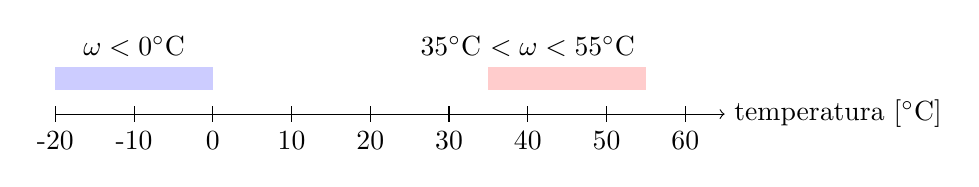
\begin{tikzpicture}
			% Draw temperature axis
			\draw[->] (0,0) -- (8.5,0) node[right] {temperatura [$^\circ$C]};
			% Add tick marks and labels every 20 degrees from -20 to 100
			\foreach \x/\label in {0/-20, 1/-10, 2/0, 3/10, 4/20, 5/30, 6/40, 7/50, 8/60} {
				\draw (\x,0.1) -- (\x,-0.1);
				\node[below] at (\x,-0.1) {\label};
			}
			% Shade measurable set: Temperature < 0°C
			\fill[blue!20] (0,0.3) rectangle (2,0.6);
			\node[above] at (1,0.6) {$\omega < 0^\circ$C};
			% Shade measurable set: 5°C < omega < 10°C
			\fill[red!20] (5.5,0.3) rectangle (7.5,0.6);
			\node[above] at (6,0.6) {$35^\circ$C $< \omega < 55^\circ$C};
			\vspace*{10mm}
		\end{tikzpicture}
			\vspace*{10mm}
		\caption{Un espacio muestral constituido por todos los valores de temperatura posibles $\omega$ 
			que pueden experimentarse en una estación FMI. Se destacan dos subconjuntos medibles de valores de temperatura, 
			denotados $\mathcal{A}^{(1)}$ y $\mathcal{A}^{(2)}$. Para cualquier 
			valor de temperatura real $\omega$, es posible determinar si $\omega \in \mathcal{A}^{(1)}$ y si $\omega \in \mathcal{A}^{(2)}$.
			} 
		\end{figure}
		En principio, los conjuntos medibles podrían elegirse libremente (por ejemplo, dependiendo de la resolución del 
		equipo de medición). Sin embargo, a menudo es útil imponer ciertos requisitos de completitud 
		en la colección de conjuntos medibles. Por ejemplo, el propio \gls{samplespace} debería ser 
		medible, y la unión de dos conjuntos medibles también debería ser medible. Estos requisitos de completitud 
		pueden formalizarse mediante el concepto de $\sigma$-álgebra (o campo $\sigma$) \cite{RudinBook}, \cite{BillingsleyProbMeasure}, \cite{durrett2010probability}. 
		Un espacio medible es un par $\big(\featurespace,\mathcal{F}\big)$ que consta de un conjunto arbitrario $\featurespace$ y una 
		colección $\mathcal{F}$ de subconjuntos medibles de $\featurespace$ que forman una $\sigma$-álgebra. 
	\\
		Véa también: \gls{probability}, \gls{samplespace}.},
	first={medible},
	text={medible} 
}



\newglossaryentry{event}
{name={evento}, 
	description={
	    Considera\index{event} una variable aleatoria $\featurevec$, definida en algún espacio de probabilidad $\mathcal{P}$, 
		que toma valores en un espacio medible $\featurespace$. Un evento $\mathcal{A} \subseteq \featurespace$ 
		es un subconjunto de $\featurespace$ tal que la probabilidad 
		$\prob{\featurevec \in \mathcal{A}}$ está bien definida. En otras palabras, la preimagen 
		$\featurevec^{-1}(\mathcal{A})$ de un evento pertenece a la $\sigma$-álgebra de $\mathcal{P}$. 
				\\
		Véa también: \gls{datapoint}, \gls{iidasspt}, \gls{rv}, \gls{probmodel}.},
	first={evento},
	firstplural={eventos},
	plural={eventos},
	text={evento} 
}


\newglossaryentry{outlier}{name={valor atípico (outlier)}, description={Muchos\index{valor atípico (outlier)} métodos de aprendizaje Automático
		están motivados por la suposición de independencia e idéntica distribución, que interpreta los puntos de datos como realizaciónes de 
		variables aleatorias iid con una distribución de probabilidad común. La suposición de independencia e idéntica distribución es útil en aplicaciones   
		donde las propiedades estadísticas del proceso de generación de datos son estacionarias (o invariantes en el tiempo) \cite{Brockwell91}. 
		Sin embargo, en algunas aplicaciones, los datos están compuestos por una mayoría de puntos de datos regulares
		que cumplen con la suposición de independencia e idéntica distribución y un pequeño número de puntos de datos que presentan propiedades estadísticas  
        fundamentalmente diferentes en comparación con los puntos de datos regulares. Nos referimos a un punto de datos que se desvía significativamente de las propiedades estadísticas  
        de la mayoría como un valor atípico (outlier). Los diferentes métodos de detección de valores atípicos utilizan distintas
        medidas para evaluar esta desviación.La teoría del aprendizaje estadístico estudia los límites fundamentales 
		sobre la capacidad de mitigar valores atípicos de manera confiable \cite{doi:10.1137/0222052,10.1214/20-AOS1961}.
		\\
		Vea también: \gls{ml}, \gls{iidasspt}, \gls{datapoint}, \gls{realization}, \gls{iid}, \gls{rv}, \gls{probdist}, \gls{data}.},
	          first={valor atípico (outlier)},text={outlier} }

\newglossaryentry{decisionregion}{name={región de decisión}, description={Consideremos\index{región de decisión} 
		un mapa de hipótesis $\hypothesis$ que entrega valores de un conjunto finito $\labelspace$. 
		Para cada valor de etiqueta (categoría) $a \in \labelspace$, la hipótesis $\hypothesis$ 
		determina un subconjunto de valores de atributos $\featurevec \in \featurespace$ que resultan 
		en el mismo resultado $\hypothesis(\featurevec)=a$. Nos referimos a este subconjunto como una región 
		de decisión de la hipótesis $\hypothesis$.
		\\
		Vea también: \gls{hypothesis}, \gls{label}, \gls{feature}.},first={región de decisión},text={región de decisión} }
		% maybe some plot here, like the one we have had in the courses?

\newglossaryentry{decisionboundary}{name={frontera de decisión}, description={Consideremos\index{frontera de decisión} un mapa de
		hipótesis $\hypothesis$ que recibe un vector de atributos  
		$\featurevec \in \mathbb{R}^{\featuredim}$ y entrega un valor de un conjunto finito $\labelspace$. 
		La frontera de decisión de $\hypothesis$ es el conjunto de vectores $\featurevec \in \mathbb{R}^{\featuredim}$ 
		que se encuentran entre diferentes regiones de decision. Más precisamente, un 
		vector $\featurevec$ pertenece a la frontera de decisión si, y solo si, cada 
		entorno $\{ \featurevec': \| \featurevec - \featurevec' \| \leq \varepsilon \}$, 
		para cualquier $\varepsilon >0$, contiene al menos dos vectores con diferentes valores de función.
		\\
		Vea tambien: \gls{hypothesis}, \gls{feature}, \gls{decisionregion}, \gls{neighborhood}.},first={frontera de decisión},text={frontera de decisión} }


\newglossaryentry{euclidspace}{name={espacio euclidiano}, description={El\index{espacio euclidiano} 
		espacio euclidiano $\mathbb{R}^{\featuredim}$ de dimensión $\featuredim \in \mathbb{N}$ consiste en 
		vectores $\featurevec= \big(\feature_{1},\ldots,\feature_{\featurelen}\big)$, con $\featuredim$ 
		entradas de valores reales $\feature_{1},\ldots,\feature_{\featuredim} \in \mathbb{R}$. Dicho espacio euclidiano
		está equipado con una estructura geométrica definida por el producto interno 
		$\featurevec^{T} \featurevec' = \sum_{\featureidx=1}^{\featuredim} \feature_{\featureidx} \feature'_{\featureidx}$ 
		entre dos vectores cualesquiera $\featurevec,\featurevec' \in \mathbb{R}^{\featuredim}$ \cite{RudinBookPrinciplesMatheAnalysis}.},first={espacio euclidiano},text={espacio euclidiano} }

\newglossaryentry{eerm}{name={minimización del riesgo empírico explicable (EERM)}, description={La\index{minimización del riesgo empírico explicable (EERM)} 
		minimización del riesgo empírico explicable (EERM) es una instancia de minimización del riesgo estructural que agrega un término de regulación a la
		perdida promedio en la funcion objetivo de ERM. 
		El término de regulación se elige para favorecer mapas de hipótesis que sean intrínsecamente 
		explicables para un usuario específico. Este usuario se caracteriza por sus predicciones proporcionadas 
		para los puntos de datos en un conjunto de entrenamiento \cite{Zhang:2024aa}.
		\\
		Vea también: \gls{srm}, \gls{regularization}, \gls{loss}, \gls{objfunc}, \gls{erm}, \gls{hypothesis}, \gls{prediction}, \gls{datapoint}, \gls{trainset}.},first={minimización del riesgo empírico explicable (EERM)},text={EERM} }
	
	
\newglossaryentry{kmeans}{name={$k$-means}, description={El\index{$k$-means} algoritmo $k$-means
		es un método de agrupamiento rígido que asigna cada punto de datos de un conjunto de datos 
		a precisamente uno de $k$ clusters diferentes. El método alterna entre actualizar 
		las asignaciones de clúster  (asignando al clúster con el medio mas cercano) y, dado estas asignaciones actualizadas 
		recalcular los medios de los clúster \cite[Ch. 8]{MLBasics}.
		\\
		Vea también: \gls{mean}, \gls{algorithm}, \gls{hardclustering}, \gls{datapoint}, \gls{dataset}, \gls{cluster}.},first={$k$-means},text={$k$-means} }
		% maybe some image here would be nice, like a step 1 -> step 2. Similar to the one in the ML course. 


\newglossaryentry{xml}{name={aprendizaje automático explicable (explainable ML)}, description={El\index{aprendizaje automático explicable (explainable ML)} 
		aprendizaje automático explicable (explainable ML) consiste en métodos de aprendizaje automático que tienen como objetivo complementar cada predicción con una explicacion 
		explícita de cómo se ha obtenido dicha predicción.La construcción de una explicacion explícita
		puede no ser necesaria si el método de aprendizaje automático utiliza un modelo lo suficientemente simple (o interpretable) \cite{rudin2019stop}.
		\\
		Vea también: \gls{prediction}, \gls{explanation}, \gls{ml}, \gls{model}.},first={aprendizaje automático explicable},text={ML explicable} }

\newglossaryentry{fmi}{name={Instituto Meteorológico de Finlandia (FMI)}, description={El\index{Instituto Meteorológico de Finlandia (FMI)}
		FMI es una agencia gubernamental responsable de recopilar y reportar datos meteorológicos en Finlandia.
		\\
		Vea también: \gls{data}.},first={Instituto Meteorológico de Finlandia (FMI)},text={FMI} }
	
\newglossaryentry{samplemean}{name={media muestral}, description={La\index{media muestral} muestra media
			$\vm \in \mathbb{R}^{\nrfeatures}$ para un conjunto de datos dado, con vectores de atributos $\featurevec^{(1)},\ldots,\featurevec^{(\samplesize)} \in \mathbb{R}^{\nrfeatures}$, 
			se define como 
			$$\vm = (1/\samplesize) \sum_{\sampleidx=1}^{\samplesize} \featurevec^{(\sampleidx)}.$$ 
			\\
			Vea también: \gls{sample}, \gls{mean}, \gls{dataset}, \gls{featurevec}.},
		first={media muestral},text={media muestral} }
	
\newglossaryentry{samplecovmtx}{name={matriz de covarianza muestral}, description={La\index{matriz de covarianza muestral} 
		matriz de matriz de covarianza muestral $\widehat{\bf \Sigma} \in \mathbb{R}^{\nrfeatures \times \nrfeatures}$ 
		para un conjunto dado vectores de atributos $\featurevec^{(1)},\ldots,\featurevec^{(\samplesize)} \in \mathbb{R}^{\nrfeatures}$ se define como 
		$$\widehat{\bf \Sigma} = (1/\samplesize) \sum_{\sampleidx=1}^{\samplesize} (\featurevec^{(\sampleidx)}\!-\!\widehat{\vm}) (\featurevec^{(\sampleidx)}\!-\!\widehat{\vm})^{T}.$$ 
		Aqui, usamos la media muestral $\widehat{\vm}$. 
		\\
		Vea también: \gls{sample}, \gls{covmtx}, \gls{featurevec}, \gls{samplemean}.},
	first={matriz de covarianza muestral},text={matriz de covarianza muestral} }

\newglossaryentry{covmtx}{name={matriz de covarianza}, 
	description={La\index{matriz de covarianza} matriz de covarianza de una variable aleatoria $\vx \in \mathbb{R}^{\featuredim}$ 
		se define como $\expect \bigg \{ \big( \vx - \expect \big\{ \vx \big\} \big)  \big(\vx - \expect \big\{ \vx \big\} \big)^{T} \bigg\}$.
		\\
		Vea también: \gls{rv}.},
	first={matriz de covarianza},text={matriz de covarianza} }
	
\newglossaryentry{highdimregime}{name={régimen de alta dimensión}, description={El\index{régimen de alta dimensión} 
		régimen de alta dimensión de minimización empírica del riesgo se caracteriza por que la dimensión efectiva del modelo
		es mayor que el tamaño de la muestra, es decir, el número de puntos de datos etiquetados en el conjunto de entrenamiento. 
		Por ejemplo, los métodos de regresión lineal operan en el régimen de alta dimensión cuando el número $\featuredim$ de atributos
		utilizados para caracterizar los puntos de datos excede el número de puntos de datos en el conjunto de entrenamiento. 
		Otro ejemplo de métodos de aprendizaje automático que operan en el régimen de alta dimensión son las red neuronal artifical grandes, que tienen
		muchos más pesos ajustables (y términos de sesgo) que el número total de puntos de datos en el conjunto de entrenamiento. 
		La estadística de alta dimensión es una línea principal reciente de la teoría de probabilidad que estudia el 
		comportamiento de los métodos de aprendizaje automático en el régimen de alta dimensión \cite{Wain2019,BuhlGeerBook}.
		\\
		Vea también: \gls{erm}, \gls{effdim}, \gls{model}, \gls{samplesize}, \gls{datapoint}, \gls{trainset}, \gls{linreg}, \gls{feature}, \gls{ml}, \gls{ann}, \gls{weights}, \gls{probability}.},
   first={régimen de alta dimensión},text={régimen de alta dimensión} }

   \newglossaryentry{covariance}
   {name={covarianza}, 
	description={La covarianza\index{covarianza} entre dos variables aleatorias reales $x$ y $y$, definidas sobre un mismo espacio de probabilidad, mide su dependencia lineal. Se define como 
			   $$
			   \cov{x}{y} = \expect\big\{ \big(x - \expect\{ x\} \big)\big(y - \expect\{y\} \big)\big\}.
			   $$
			   Una covarianza positiva indica que $x$ y $y$ tienden a aumentar juntos, mientras que una covarianza negativa sugiere que uno tiende a aumentar cuando el otro disminuye. Si $\cov{x}{y} = 0$, se dice que las \glspl{rv} son no correlacionadas, aunque esto no implica necesariamente que sean estadísticamente independientes. Véa la Figura~\ref{fig:covariance-examples_dict} para ilustraciones visuales.
		   \begin{figure}[H]
		   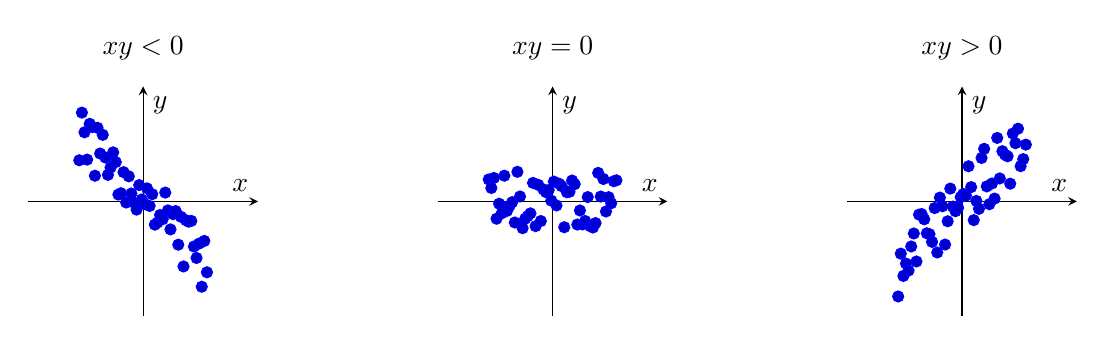
\begin{tikzpicture}
			% Negative covariance
		   \begin{scope}[shift={(0,0)}]
			   \begin{axis}[
				   width=4.5cm, height=4.5cm,
							title={$\cov{x}{y} <0$},
				   xlabel={$x$}, ylabel={$y$},
				   xmin=-3, xmax=3, ymin=-3, ymax=3,
				   xtick=\empty, ytick=\empty,
				   axis lines=middle, enlargelimits
				   ]
				   \addplot+[only marks, mark=*, samples=50, domain=-2:2] 
				   ({x}, {-x + rand});
			   \end{axis}
		   \end{scope}
		   % Zero covariance
		   \begin{scope}[shift={(5.2cm,0)}]
			   \begin{axis}[
				   width=4.5cm, height=4.5cm,
					title={$\cov{x}{y} =0$}, xlabel={$x$}, ylabel={$y$},
				   xmin=-3, xmax=3, ymin=-3, ymax=3,
				   xtick=\empty, ytick=\empty,
				   axis lines=middle, enlargelimits
				   ]
				   \addplot+[only marks, mark=*, samples=50, domain=-2:2] 
				   ({x}, {rand});
			   \end{axis}
		   \end{scope}
		   % Positive covariance
		   \begin{scope}[shift={(10.4cm,0)}]
			   \begin{axis}[
				   width=4.5cm, height=4.5cm,
					title={$\cov{x}{y} > 0$},
				   xlabel={$x$}, ylabel={$y$},
				   xmin=-3, xmax=3, ymin=-3, ymax=3,
				   xtick=\empty, ytick=\empty,
				   axis lines=middle, enlargelimits
				   ]
				   \addplot+[only marks, mark=*, samples=50, domain=-2:2] 
				   ({x}, {x + rand});
			   \end{axis}
		   \end{scope}
		   \end{tikzpicture}
			   \caption{Diagramas de dispersion ilustrando realizaciónes de tres modelos de probabilidad diferentes para dos
				  variables aleatorias reales con diferentes valores de covarianza: negativo (izquierda), cero (centro), y positivo (derecha).}
			   \label{fig:covariance-examples_dict}
		   \end{figure}
		   },
	   first={covarianza},
	   text={covarianza} 
   }


\newglossaryentry{gmm}{name={modelo de mezcla gaussiana (GMM)}, description={Un GMM\index{modelo de mezcla gaussiana (GMM)} 
		es un tipo particular de modelo de probabilidad para un vector numérico $\featurevec$ (por ejemplo, 
		los atributos de un punto de datos). Dentro de un GMM, el vector  $\featurevec$ se extrae de una  
		distribución normal multivariante $p^{(\clusteridx)} = \mvnormal{\meanvec{\clusteridx}}{\covmtx{\clusteridx}}$ seleccionada aleatoriamente,
		con $\clusteridx = I$. El índice $I \in \{1,\ldots,\nrcluster\}$ es una variable aleatoria con probabilidades $\prob{I=\clusteridx} = p_{\clusteridx}$.
	    Ten en cuenta que un GMM se parametriza por la probabilidad $p_{\clusteridx}$, el 
		vector medio $\clustermean{\clusteridx}$, y la matriz de covarianza $\bf\Sigma^{(\clusteridx)}$ para cada $\clusteridx=1,\ldots,\nrcluster$. 
		Los GMM se utilizan ampliamente para agrupamiento, estimación de densidad y como un modelo generativo. 
		\\
		Vea también: \gls{probmodel}, \gls{feature}, \gls{datapoint}, \gls{mvndist}, \gls{rv}, \gls{mean}, \gls{covmtx}, \gls{clustering}, \gls{model}.},first={modelo de mezcla gaussiana (GMM)},text={GMM} }
 
\newglossaryentry{maxlikelihood}{name={máxima verosimilitud}, description={
		Considera\index{máxima verosimilitud} puntos de datos $\dataset=\big\{ \datapoint^{(1)}, \ldots, \datapoint^{(\samplesize)} \}$ 
		que se interpretan como las realizaciónes de variables aleatorias iid con una distribución de probabilidad común $\prob{\datapoint; \weights}$ que 
		depende de los parametros del modelo $\weights \in \mathcal{W} \subseteq \mathbb{R}^{n}$. 
		Los métodos de máxima verosimilitud aprenden los parametros del modelo $\weights$ al maximizar 
		la probabilidad (densidad) $\prob{\dataset; \weights} = \prod_{\sampleidx=1}^{\samplesize} \prob{\datapoint^{(\sampleidx)}; \weights}$ 
		del conjunto de datos observado. Por lo tanto, el estimador de máxima verosimilitud es una 
		solución al problema de optimización $\max_{\weights \in \mathcal{W}} \prob{\dataset; \weights}$.
		\\
		Vea también: \gls{datapoint}, \gls{realization}, \gls{iid}, \gls{rv}, \gls{probdist}, \glspl{modelparam}, \gls{maximum}, \gls{dataset}.},first={máxima verosimilitud},text={máxima verosimilitud}}



\newglossaryentry{em}{name={esperanza-maximización (EM)}, description={
		\index{esperanza-maximización (EM)} 
		Considera un modelo de probabilidad $\prob{\datapoint; \weights}$ para los puntos de datos $\dataset$ generados en alguna 
		aplicación de aprendizaje Automático. El estimador de maxima verosimilitud para los parametros del modelo $\weights$ se obtienen maximizando
		$\prob{\dataset; \weights}$. Sin embargo, el problema de optimización resultante puede ser computacionalmente 
		desafiante. El algoritmo de expectativa-maximización (EM) aproxima el estimador de maxima verosimilitud introduciendo una  
		variable aleatoria latente $\vz$ de modo que maximizar  $\prob{\dataset,\vz; \weights}$ sea más fácil \cite{BishopBook,hastie01statisticallearning,GraphModExpFamVarInfWainJor}. Dado que 
		no observamos $\vz$, necesitamos estimarlo a partir del conjunto de datos observado $\dataset$ 
		utilizando una esperanza condicional. La estimación resultante $\widehat{\vz}$ se utiliza para 
		calcular una nueva estimación $\widehat{\weights}$ resolviendo $\max_{\weights} \prob{\dataset, \widehat{\vz}; \weights}$. 
		El punto clave es que la esperanza condicional $\widehat{\vz}$ depende de los parametros del modelo $\widehat{\weights}$, 
		que hemos actualizado en función de $\widehat{\vz}$. Por lo tanto, debemos volver a calcular $\widehat{\vz}$, 
		lo que a su vez resulta en una nueva elección $\widehat{\weights}$ para los parametros del modelo.  En la práctica, 
		repetimos el cálculo de la esperanza condicional (es decir, el E-step) y la actualización 
		de los parametros del modelo (es decir, the M-step)  hasta que se cumpla algún criterio de parada.
		\\
		Vea también: \gls{probmodel}, \gls{datapoint}, \gls{ml}, \gls{maxlikelihood}, \glspl{modelparam}, \gls{rv}, \gls{dataset}, \gls{expectation}, \gls{stopcrit}. },first={EM},text={EM}}

\newglossaryentry{ppca}{name={análisis de componentes principales probabilístico (PPCA)}, description={El análisis de componentes principales probabilístico (PPCA)\index{análisis de componentes principales probabilístico (PPCA)} 
		extiende el pca básico mediante el uso de un modelo de probabilidad para los puntos de datos. El modelo de probabilidad de PPCA
		reduce la tarea de reducción de dimensionalidad a un problema de estimación que se puede resolver utilizando métodos de esperanza-maximización.
		\\
		Vea también: \gls{pca}, \gls{probmodel}, \gls{datapoint}, \gls{em}.},first={análisis de componentes principales probabilístico (PPCA)},text={PPCA}}
	
\newglossaryentry{polyreg}{name={regresión polinómica}, description={La \index{regresión polinómica} regresión polinómica es una instancia de ERM que aprende un mapa de 
hipótesis polinómica para predecir una etiqueta numérica a partir de los atributos numéricos de un punto de datos. 
Para puntos de datos caracterizados por un único atributo numérico, la regresión polinómica utiliza el espacio de hipótesis
\[
\hypospace^{(\rm poly)}_{\nrfeatures} \defeq \left\{ \hypothesis(x) = \sum_{\featureidx=0}^{\nrfeatures-1} x^{\featureidx} \weight_{\featureidx} \right\}.
\]
La calidad de una hipótesis polinómica  se mide mediante la perdida de error cuadrático promedio 
incurrida en un conjunto de puntos de datos etiquetados (al que nos referimos como el conjunto de entrenamiento).
			\\
		Vea también: \gls{regression}, \gls{hypothesis}, \gls{label}, \gls{feature}, \gls{datapoint}, \gls{hypospace}, \gls{sqerrloss}, \gls{labeled datapoint}, \gls{trainset}.},first={regresión polinómica},text={regresión polinómica}}

\newglossaryentry{linreg}{name={regresión lineal}, description={La\index{regresión lineal} 
		regresión lineal tiene como objetivo aprender un mapa de hipótesis lineal para predecir una etiqueta numérica basada en los 
		atributos numéricos de un punto de datos. La calidad de un mapa de hipótesis lineal se mide utilizando el promedio de 
		error cuadrado medio incurrido en un conjunto de puntos de datos etiquetados, 
		al que nos referimos como el conjunto de datos.
		\\
		Vea también: \gls{regression}, \gls{hypothesis}, \gls{label}, \gls{feature}, \gls{datapoint},  \gls{sqerrloss}, \gls{labeled datapoint}, \gls{trainset}.},first={regresión lineal},text={regresión lineal}}
        
\newglossaryentry{ridgeregression}{name={regresión ridge}, description={La\index{regresión ridge} 
		regresión ridge aprende los pesos $\weights$ de un mapa de hipótesis lineal $\hypothesis^{(\weights)}(\featurevec)= \weights^{T} \featurevec$. La calidad de una elección particular para los parametros del modelo $\weights$ se mide por la suma de dos componentes. 
		El primer componente es el promedio de error cuadrado medio incurrido por $\hypothesis^{(\weights)}$ en un conjunto de
		puntos de datos etiquetados (es decir, el conjunto de entrenamiento). El segundo componente es el cuadrado de la 
		norma Euclidiana escalada $\regparam \| \weights \|^{2}_{2}$ con un parámetro de regulación
		$\regparam > 0$. Agregar $\regparam \| \weights \|^{2}_{2}$ al promedio de
	    medio cuadrado medio es equivalente a reemplazar cada punto de datos original por la realización
	    de (infinitos) variables aleatorias iid centrados alrededor de estos puntos de datos (vea regulación).
		\\
		Vea también: \gls{regression}, \gls{weights}, \gls{hypothesis}, \glspl{modelparam}, \gls{sqerrloss}, \gls{labeled datapoint}, \gls{trainset}, \gls{norm}, \gls{regularization}, \gls{datapoint}, \gls{realization}, \gls{iid}, \gls{rv}.},first={regresión ridge},text={regresión ridge}}


\newglossaryentry{expectation}{name={esperanza}, description={
		Consideremos\index{expectation} un vector de atributos numérico $\featurevec \in \mathbb{R}^{\featuredim}$ 
		que interpretamos como la realización de una variable aleatoria con una distribución de probabilidad $p(\featurevec)$. 
		La esperanza de $\featurevec$ se define como la integral $\expect \{ \featurevec \} \defeq \int \featurevec p(\featurevec)$ \cite{HalmosMeasure,BillingsleyProbMeasure,RudinBookPrinciplesMatheAnalysis}. Nótese que
		la esperanza solo está definida si esta integral existe, es decir, si la variable aleatoria es integrable.\cite{RudinBookPrinciplesMatheAnalysis}, \cite{BillingsleyProbMeasure}, \cite{HalmosMeasure}. 
		Fig. \ref{fig_expect_discrete} ilustra la esperanza de una variable aleatoria  discreta $x$ que toma valores
		solo de un conjunto finito.
	   \begin{figure}[H]
		   \begin{center}
		   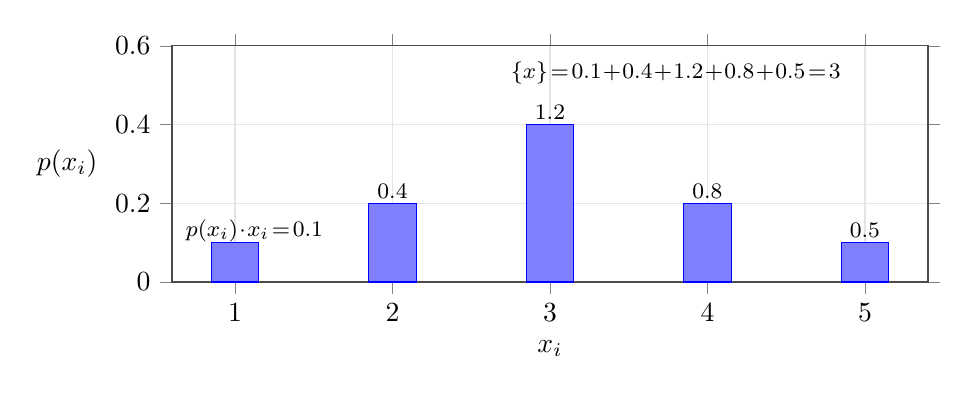
\begin{tikzpicture}
	\begin{axis}[
		ybar,
		y=5cm,
		x=2cm,                          % ⬅️ Controls spacing between bars
		bar width=0.6cm,                   % ⬅️ Controls bar thickness
	%	bar shift=-0.5cm,                % ⬅️ Center bars (=-0.5 * bar width)
		xlabel={$x_i$},
		clip=false,
		ylabel={$p(x_i)$},
		y label style={rotate=-90, anchor=west, xshift=-1cm},
		xtick={1,2,3,4,5},
		ymin=0, ymax=0.6,
		grid=both,
		major grid style={gray!20},
		tick align=outside,
		axis line style={black!70},
		]
		\addplot+[ybar, fill=blue!50] coordinates {
			(1,0.1) 
			(2,0.2) 
			(3,0.4) 
			(4,0.2)
			(5,0.1)
		};
		% Manual textboxes above bars
		\node[font=\footnotesize,xshift=7pt] at (axis cs:1,0.13) {$p(x_i)\!\cdot\!x_i\!=\!0.1$};
		\node[font=\footnotesize]at (axis cs:2,0.23) {$0.4$};
		\node[font=\footnotesize]at (axis cs:3,0.43) {$1.2$};
		\node[font=\footnotesize] at (axis cs:4,0.23) {$0.8$};
		\node[font=\footnotesize]at (axis cs:5,0.13) {$0.5$};
		\node[font=\footnotesize]at (axis cs:3.8,0.53) {$\expect\{x\}\!=\!0.1\!+\!0.4\!+\!1.2\!+\!0.8\!+\!0.5\!=\!3$};
	\end{axis}
	\end{tikzpicture}
	\end{center}
	\vspace*{-5mm}
	\caption{La esperanza de una variable aleatoria discreta $x$ se obtiene sumando sus posibles valores $x_{i}$,ponderados por la correspondiente probabilidad $p(x_i) = \prob{x= x_i}$. \label{fig_expect_discrete}}
	 \end{figure}
			Vea también: \gls{featurevec}, \gls{realization}, \gls{rv}, \gls{probdist}, \gls{probability}.},
	first={esperanza},
	text={esperanza}
	}
	

\newglossaryentry{logreg}{name={regresión logística}, description={La\index{regresión logística} regresión logística aprende un 
		mapeo hipótesis lineal (o clasificador) $\hypothesis(\featurevec) = \weights^{T} \featurevec$ 
		para predecir una etiqueta binaria $\truelabel$ basada en el vector de atributos númerico $\featurevec$ de 
		algun punto de datos. La calidad de un mapeo hipótesis lineal se mide por el promedio de la pérdida logística 
		sobre algunos puntos de etiquetados (es decir, el conjunto de entrenamiento).
		\\
		Vea también: \gls{regression}, \gls{hypothesis}, \gls{classifier}, \gls{label}, \gls{featurevec}, \gls{datapoint}, \gls{logloss}, \gls{labeled datapoint}, \gls{trainset}.},
		first={regresión logística},text={regresión logística}}
	
		\newglossaryentry{logloss}
	{name={pérdida logística}, 
		description={Considérese\index{pérdida logística} 
			un punto de datos caracterizado por los atributos $\featurevec$ y una etiqueta binaria $\truelabel \in \{-1,1\}$. 
			Usamos una hipótesis con valores reales $\hypothesis$ para predecir la etiqueta $\truelabel$ 
			a partir de los atributos $\featurevec$. La perdida logística incurrida por esta predicción se 
			define como
		\begin{equation} 
			\label{equ_log_loss_gls_dict}
			\lossfunc{(\featurevec,\truelabel)}{\hypothesis} \defeq  \log\, ( 1 + \exp\,(- \truelabel \hypothesis(\featurevec))).
		\end{equation}
		\begin{figure}[H]
		\begin{center}
			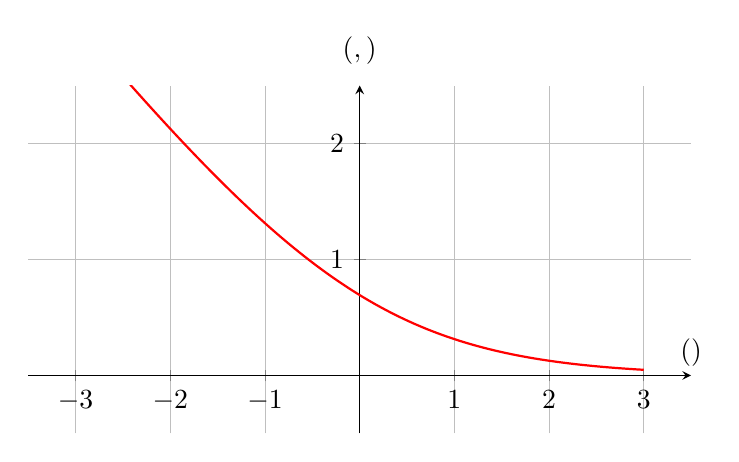
\begin{tikzpicture}
				\begin{axis}[
					axis lines=middle,
					xlabel={$\truelabel\hypothesis(\featurevec)$},
					ylabel={$\lossfunc{(\featurevec,\truelabel)}{\hypothesis}$},
					xlabel style={at={(axis description cs:1.,0.3)}, anchor=north},
					ylabel style={at={(axis description cs:0.5,1.1)}, anchor=center},
					xmin=-3.5, xmax=3.5,
					ymin=-0.5, ymax=2.5,
					xtick={-3, -2, -1, 0, 1, 2, 3},
					ytick={0, 1, 2},
					domain=-3:3,
					samples=100,
					width=10cm, height=6cm,
					grid=both,
					major grid style={line width=.2pt, draw=gray!50},
					minor grid style={line width=.1pt, draw=gray!20},
					legend pos=south west
					]
						\addplot [red, thick] {ln(1 + exp(-x))};    
				\end{axis}
			\end{tikzpicture}
			\caption{La perdida logística incurrida por la predicción $\hypothesis(\featurevec) \in \mathbb{R}$ 
				para un punto de datos con etiqueta $\truelabel \in \{-1,1\}$.}
			\label{fig_logloss_dict}
		\end{center}
		\end{figure}
		Nótese que la expresión \eqref{equ_log_loss_gls_dict} 
		para la perdida logística aplica únicamente para el espacio de etiquetas $\labelspace = \{ -1,1\}$ y cuando se utiliza 
		la regla de umbral dada en \eqref{equ_def_threshold_bin_classifier_dict}. 
			\\
			Véa también: \gls{datapoint}, \gls{feature}, \gls{label}, \gls{hypothesis}, \gls{loss}, \gls{prediction}, \gls{labelspace}.},
		first={pérdida logística},
		text={pérdida logística}
	}

	
\newglossaryentry{hingeloss}{name={pérdida de hinge}, description={Consideremos\index{pérdida de hinge} un punto de datos
		caracterizado por un vector de atributos $\featurevec \in \mathbb{R}^{\featuredim}$ y una
		etiqueta binaria $\truelabel \in \{-1,1\}$. La perdida de hinge incurrida por un 
		mapa de hipótesis $\hypothesis(\featurevec)$ se define como
		\begin{equation} 
			\label{equ_hinge_loss_gls_dict}
				\lossfunc{(\featurevec,\truelabel)}{\hypothesis} \defeq \max \{ 0 , 1 - \truelabel \hypothesis(\featurevec) \}. 
			\end{equation}
			\begin{figure}[H]
			\begin{center}
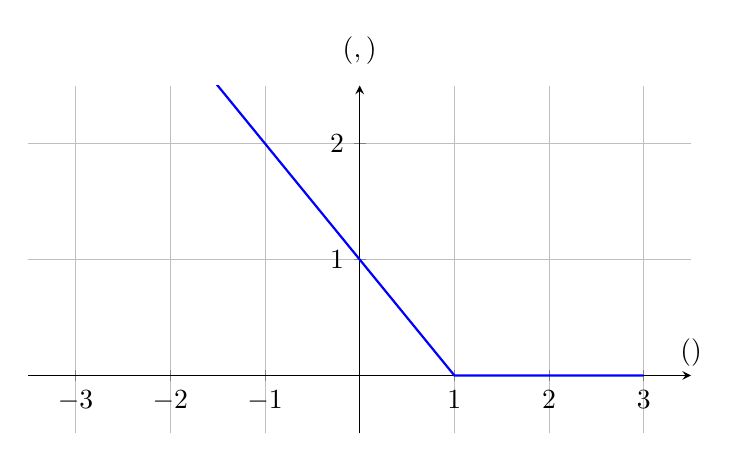
\begin{tikzpicture}
    \begin{axis}[
        axis lines=middle,
        xlabel={$\truelabel\hypothesis(\featurevec)$},
        ylabel={$\lossfunc{(\featurevec,\truelabel)}{\hypothesis}$},
 	xlabel style={at={(axis description cs:1.,0.3)}, anchor=north},  % Adjusted to be relative to axis end
        ylabel style={at={(axis description cs:0.5,1.1)}, anchor=center}, % Corrected to vertical position, rotated for readability
        xmin=-3.5, xmax=3.5,
        ymin=-0.5, ymax=2.5,
        xtick={-3, -2, -1, 0, 1, 2, 3},
        ytick={0, 1, 2},
        domain=-3:3,
        samples=100,
        width=10cm, height=6cm,
        grid=both,
        major grid style={line width=.2pt, draw=gray!50},
        minor grid style={line width=.1pt, draw=gray!20},
        legend pos=south west % Positions legend at the bottom left
    ]
        \addplot[blue, thick] {max(0, 1-x)};
     %   \addlegendentry{$\max(0, 1-x)$}
    \end{axis}
\end{tikzpicture}
\caption{La perdida de Hinge incurrida por la predicción $\hypothesis(\featurevec) \in \mathbb{R}$ 
para un punto de datos con etiqueta $\truelabel \in \{-1,1\}$. Una variante regularizada de la perdida de hinge
es usada por la maquina de vectores de soporte \cite{LampertNowKernel}.}
\label{fig_hingeloss_dict}
\end{center}
\end{figure} 	    
		Vea también: \gls{datapoint}, \gls{featurevec}, \gls{label}, \gls{loss}, \gls{hypothesis}, \gls{svm}.},
		first={pérdida de hinge},
		text={pérdida de hinge}}

\newglossaryentry{iidasspt}{name={suposición de independencia e idéntica distribución (suposición i.i.d.)}, description={La suposición iid 
		\index{suposición de independencia e idéntica distribución (suposición i.i.d.)} interpreta los puntos de datos de un conjunto de datos como las 
		realizaciónes de variables aleatorias iid.
		\\
		Vea también: \gls{iid}, \gls{datapoint}, \gls{dataset}, \gls{realization}, \gls{rv}.},first={suposición de independencia e idéntica distribución (suposición i.i.d.)},text={suposición i.i.d.} }


\newglossaryentry{hypospace}
{name={espacio de hipótesis}, plural={espacios de hipótesis},
description={Un espacio de hipótesis\index{espacio de hipótesis} es un modelo matemático 
que caracteriza la capacidad de aprendizaje de un método de aprendizaje automático. El objetivo de dicho método es 
aprender una mapa de hipótesis que asigne los atributos de un punto de datos a una 
prediccion de su etiqueta. Dado un recurso computacional finito, un método práctico de aprendizaje automático 
normalmente explora solo un subconjunto restringido de todos los posibles mapas desde el espacio de atributos
al espacio de etiquetas. A este subconjunto restringido se le denomina espacio de hipótesis $\hypospace$ 
asociado al método de aprendizaje automático.
Para el análisis de un método dado de aprendizaje automático, la elección del espacio de hipótesis $\hypospace$ no es única: 
cualquier superconjunto que contenga todos los mapas que el método puede aprender también es un espacio de 
hipótesis válido.
\begin{figure}[H]
\begin{center}
	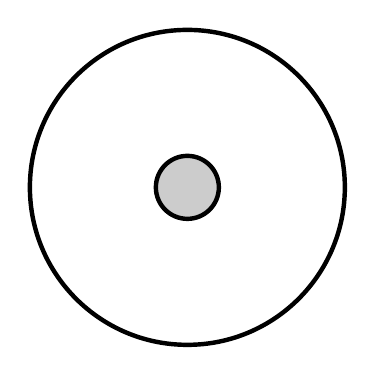
\begin{tikzpicture}[allow upside down, scale=0.4]
		\node [below] at (5,-3) {$\labelspace^{\featurespace}$};
		\draw [ultra thick] (5,0) circle (5cm);
		\draw [ultra thick,fill=black!20] (5,0) circle (1cm);
		\node [] at (5,0) {$\hypospace$};
	\end{tikzpicture}
\end{center}
\caption{El espacio de hipótesis $\hypospace$ de un método de aprendizaje automático es un subconjunto 
(típicamente muy pequeño) del conjunto $\labelspace^{\featurespace}$ (típicamente muy grande) 
de todos los posibles mapas desde el espacio de atributos $\featurespace$ al espacio de etiquetas $\labelspace$.}
\end{figure}
Desde la perspectiva de la ingeniería de aprendizaje automático, por otro lado, el espacio de hipótesis $\hypospace$ 
es una decisión de diseño en métodos basados en ERM. Esta decisión puede guiarse por los recursos 
computacionales disponibles y por los aspectos estadísticos. Por ejemplo, si es factible aplicar operaciones de 
matriz eficientes y existe una relación aproximadamente lineal entre atributos y etiquetas, 
un modelo lineal puede ser una elección útil para $\hypospace$.\\
Véa también: \gls{hypothesis}, \gls{model}, \gls{map}, \gls{linmodel}.},
first={espacio de hipótesis},
text={espacio de hipótesis}
}

		
		\newglossaryentry{model}
		{name={modelo}, plural={modelos}, 
			description={El estudio y diseño de métodos de aprendizaje automático suele basarse en un modelo matemático \cite{bender1978mathematical}. 
			Quizás el ejemplo más utilizado de un modelo matemático en aprendizaje automático es un espacio de hipótesis. 
			Un espacio de hipótesis consiste en mapas de hipótesis que son utilizados por un método de aprendizaje automático 
			para predecir etiquetas a partir de los atributos de los puntos de datos. Otro tipo importante de 
			modelo matemático es un modelo de probabilidad, que consiste en distribuciones de probabilidad que describen 
			cómo se generan los puntos de datos. A menos que se indique lo contrario, utilizamos el término modelo para 
			referirnos específicamente al espacio de hipótesis subyacente a un método de aprendizaje automatico.
			 \\
			Véa también: \gls{hypospace}, \gls{probmodel}, \gls{probdist}.
			\begin{figure}[H]
			\centering
			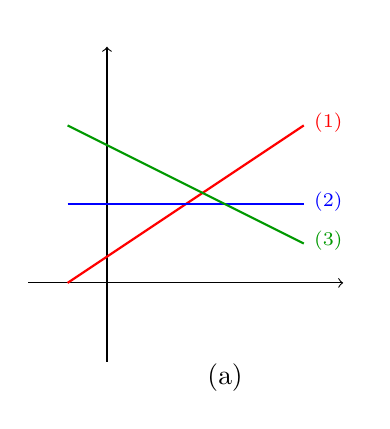
\begin{tikzpicture}[scale=1]
			\draw[->] (-1,0) -- (3,0) node[right] {$\feature$};
			\draw[->] (0,-1) -- (0,3) node[above] {$\truelabel$};
			\draw[thick, red] (-0.5,0) -- (2.5,2) node[right] {$\hypothesis^{(1)}$};
			\draw[thick, blue] (-0.5,1) -- (2.5,1) node[right] {$\hypothesis^{(2)}$};
			\draw[thick, green!60!black] (-0.5,2) -- (2.5,0.5) node[right] {$\hypothesis^{(3)}$};
			\node at (1.5,-1.2) {(a)};
			\end{tikzpicture}
			\hspace{2cm}
			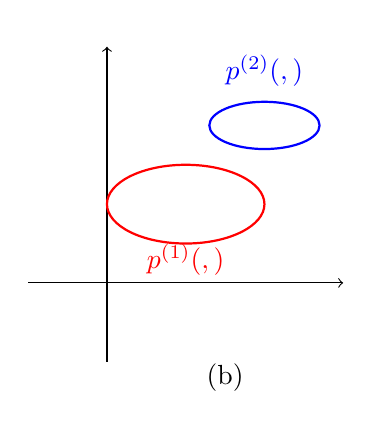
\begin{tikzpicture}[scale=1]
			\draw[->] (-1,0) -- (3,0) node[right] {$\feature$};
			\draw[->] (0,-1) -- (0,3) node[above] {$\truelabel$};
			\draw[thick, red] (1,1) ellipse [x radius=1, y radius=0.5];
			\draw[thick, blue] (2,2) ellipse [x radius=0.7, y radius=0.3];
			\node[red] at (1,0.3) {$p^{(1)}(\feature,\truelabel)$};
			\node[blue] at (2,2.7) {$p^{(2)}(\feature,\truelabel)$};
			\node at (1.5,-1.2) {(b)};
			\end{tikzpicture}
			\caption{Dos tipos de modelos matemáticos utilizados en aprendizaje automático: (a) un espacio de hipótesis que consiste en 
			tres mapas lineales; (b) un modelo de probabilidad compuesto por distribuciones de probabilidad sobre el plano definido por 
			los valores de atributos y etiqueta de un punto de datos.}
			\end{figure}
			},
			first={modelo},
			text={modelo} 
		}
		

\newglossaryentry{modelparams}{name={parámetros del modelo}, 
	description={Los parametros\index{parámetros del modelo} de un modelo son cantidades que se utilizan para seleccionar un mapa de hipótesis específico dentro de un modelo. 
	Podemos pensar en una lista de parametros del modelo como un identificador único para un mapa de hipótesis, 
	similar a cómo un número de seguridad social identifica a una persona en Finlandia.
	\\
		Vea también: \gls{model}, \gls{parameters}, \gls{hypothesis}.},
	first={parámetros del modelo},text={parámetros del modelo} }

\newglossaryentry{ai}{name={inteligencia artificial (IA)}, description={
	La IA\index{inteligencia artificial (IA)} se refiere a sistemas que se comportan de manera racional en el sentido de maximizar una recompensa a largo plazo. 
	El enfoque basado en aprendizaje automático para la IA consiste en entrenar un modelo para predecir acciones óptimas. 
	Estas predicciones se calculan a partir de observaciones sobre el estado del entorno. 
	La elección de la funcion de perdida distingue las aplicaciones de IA de las aplicaciones de aprendizaje automático más básicas. 
	Los sistemas de IA rara vez tienen acceso a un conjunto de entrenamiento etiquetado que permita medir la perdida promedio para cualquier posible elección de parametros del modelo. 
	En su lugar, los sistemas de IA utilizan señales de recompensa observadas para obtener una estimación puntual de la perdida incurrida por la elección actual de parametros del modelo.
	\\
		Vea también: \gls{reward}, \gls{ml}, \gls{model}, \gls{lossfunc}, \gls{trainset}, \gls{loss}, \glspl{modelparam}.},first={AI},text={AI} }



		\newglossaryentry{mdp}
		{name={proceso de decisión de Markov (MDP)},
		 description={
			Un MDP\index{proceso de decisión de Markov (MDP)} es una estructura matemática que puede 
			utilizarse para estudiar aplicaciones de aprendizaje por refuerzo. Un MDP formaliza cómo las señales de recompensa 
			dependen de las predicciones (y las acciones correspondientes) realizadas por un método de aprendizaje por refuerzo. 
			Formalmente, un MDP es un tipo específico de proceso estocástico definido por:
			\begin{itemize}
			\item un espacio de estados $\mathcal{S}$,
			\item un espacio de acciones $\mathcal{A}$ (cada acción $a \in \mathcal{A}$ corresponde a una 
				prediccion específica realizada por el método de aprendizaje por refuerzo),
			\item una función de transición $\prob{s' \mid s, a}$ que especifica la distribución de probabilidad sobre el 
				siguiente estado $s' \in \mathcal{S}$, dado el estado actual $s \in \mathcal{S}$ y la acción $a \in \mathcal{A}$,
			\item una función de recompensa $\reward(s, a) \in \mathbb{R}$ que asigna una recompensa numérica a cada 
				par estado-acción.
			\end{itemize}
			La propiedad definitoria de un MDP es la propiedad de Markov: el siguiente estado $s'$ y la recompensa
			dependen únicamente del estado actual $s$ y de la acción $a$, y no de todo el historial de interacción.
			},
		 first={mdp},
		 text={mdp} 
		}
		


\newglossaryentry{reward}{name={recompensa}, description={Una recompensa se refiere a alguna\index{recompensa} 
	cantidad observada (o medida) que nos permite estimar la perdida incurrida por la predicción
	(o decisión) de una hipótesis $\hypothesis(\featurevec)$. Por ejemplo, en una 
	aplicación de aprendizaje automático para vehículos autónomos, $\hypothesis(\featurevec)$ podría representar 
	la dirección actual del volante de un vehículo. Podríamos construir una recompensa a partir de 
	las mediciones de un sensor de colisión que indique si el vehículo se dirige hacia 
	un obstáculo. Definimos una recompensa baja para la dirección del volante 
	$\hypothesis(\featurevec)$ si el vehículo se mueve peligrosamente hacia un obstáculo.
	\\
		Vea también: \gls{loss}, \gls{prediction}, \gls{hypothesis}, \gls{ml}.},
	first={recompensa}, text={recompensa}} 

\newglossaryentry{hardclustering}{name={agrupamiento rígido}, description={El agrupamiento rígido\index{agrupamiento rígido} 
	se refiere a la tarea de dividir un conjunto dado de puntos de dastos en (pocos)clusteres no superpuestos. 
	El método de agrupamiento rígido más utilizado es k-means.
	\\
		Vea también: \gls{clustering}, \gls{datapoint}, \gls{cluster}, \gls{kmeans}.},first={agrupamiento rígido},text={agrupamiento rígido} }
	
\newglossaryentry{softclustering}{name={agrupamiento suave}, description={El agrupamiento suave\index{agrupamiento suave} 
	se refiere a la tarea de dividir un conjunto dado de puntos de datos en (pocos) clusteres superpuestos. 
	Cada punto de datos se asigna a varios clusteres diferentes con diversos grados de pertenencia. 
	Los métodos de agrupamiento suave determinan el grado de pertenencia (o asignación suave a un clúster) 
	para cada punto de datos y cada clúster. Un enfoque fundamentado para el agrupamiento suave 
	consiste en interpretar los puntos de datos como realizaciónes iid de un modelo de mezcla gaussiana. 
	De este modo, se obtiene una elección natural para el grado de pertenencia como la probabilidad 
	condicional de que un puntos de datos pertenezca a un componente específico de la mezcla.
	\\
	Vea tambien: \gls{clustering}, \gls{datapoint}, \gls{cluster}, \gls{dob}, \gls{iid}, \gls{realization}, \gls{gmm}, \gls{probability}.},first={agrupamiento suave},text={agrupamiento suave} }


	\newglossaryentry{kroneckerproduct}
	{name={producto de Kronecker}, 
		description={El producto de Kronecker\index{producto de Kronecker} de dos matrices $\mA \in \mathbb{R}^{m \times n}$ 
		y $\mB \in \mathbb{R}^{p \times q}$ es una matriz por bloques denotada como $\mA \otimes \mB$ 
		y definida como \cite{GolubVanLoanBook}, \cite{HornMatAnalysis}
		\[
		\mA \otimes \mB =
		\begin{bmatrix}
			a_{11}\mB & \cdots & a_{1n}\mB \\
			\vdots & \ddots & \vdots \\
			a_{m1}\mB & \cdots & a_{mn}\mB
		\end{bmatrix}
		\in \mathbb{R}^{mp \times nq}.
		\]
		El producto de Kronecker es un caso particular del producto tensorial para matrices y se 
		utiliza ampliamente en estadística multivariada, álgebra lineal y modelos estructurados de aprendizaje automático. 
		Satisface la identidad $(\mA \otimes \mB)(\vx \otimes \vy) = (\mA\vx) \otimes (\mB\vy)$ 
		para vectores $\vx$ y $\vy$ de dimensiones compatibles.
		\\
		Véa también: \gls{ml}, \gls{model}. },
		first={producto de Kronecker},
		text={producto de Kronecker} 
	}
	
		
\newglossaryentry{clustering}{name={agrupamiento}, description={Los métodos de agrupamiento\index{agrupamiento} 
	descomponen un conjunto dado de puntos de datos en pocos subconjuntos, que se denominan clústers. 
	Cada clúster está compuesto por puntos de dastos que son más similares entre sí que con respecto a 
	los puntos de datos fuera del clúster. Los diferentes métodos de agrupamiento utilizan 
	distintas medidas de similitud entre puntos de datos y diferentes formas de representación de los clústers. 
	El método de agrupamiento k-means utiliza el vector de atributo promedio (media del clúster) 
	de un clúster como su representante. Un método popular de agrupamiento suave basado en el modelo de mezcla gaussiana 
	representa un clúster mediante una distribución normal multivariante.
	\\
		Vea también: \gls{datapoint}, \gls{cluster}, \gls{kmeans}, \gls{feature}, \gls{mean}, \gls{softclustering}, \gls{gmm}, \gls{mvndist}.},first={agrupamiento},text={agrupamiento} }
	
\newglossaryentry{cluster}{name={clúster}, description={Un\index{clúster} clúster es un subconjunto de 
	puntos de datos que son más similares entre sí que a los puntos de datos fuera del clúster. 
	La medida cuantitativa de similitud entre los puntos de datos es una decisión de diseño. 
	Si los puntos de datos se caracterizan por vectores de atributos euclidianos 
	$\featurevec \in \mathbb{R}^{\nrfeatures}$, podemos definir la similitud entre dos puntos de datos
	a través de la distancia euclidiana entre sus vectores de atributos.
	Un ejemplo de tal clúster es.~\ref{fig:clusters}.\\
		\begin{figure}[H]
		\centering
		\begin{tikzpicture}
		\pgfplotsset{compat=1.18}
		\begin{axis}[
		    width=10cm,
		    height=8cm,
		    xlabel={$x_1$},
		    ylabel={$x_2$},
		    title={Clusters of Data Points},
		    xmin=0, xmax=10,
		    ymin=0, ymax=10,
		    axis lines=left,
		    legend style={at={(0.5,-0.25)}, anchor=north, legend columns=3}
		]
		% Cluster 1 
		\addplot[only marks, color=blue, mark=*, mark size=3pt] coordinates {
		    (1,1) (2,1.2) (1.8,2) (2.2,1.5) (1.5,2.5)
		};
		% Cluster 2 
		\addplot[only marks, color=red, mark=square*, mark size=3pt] coordinates {
		    (7,8) (8,7.5) (7.5,8.5) (8.2,7.8) (7.7,7)
		};
		% Cluster 3 
		\addplot[only marks, color=green!60!black, mark=triangle*, mark size=3pt] coordinates {
		    (5,3) (5.5,3.2) (5.2,2.8) (4.8,3.5) (5.1,3.1)
		};
		\legend{Cluster 1, Cluster 2, Cluster 3}
		\end{axis}
		\end{tikzpicture}
		\caption{Ilustración de tres clústers en un espacio de atributos bidimensional. Cada clúster agrupa puntos de datos que son más similares entre sí que con aquellos en otros clusters, basándose en la distancia euclidiana.}
		\label{fig:clusters}
		\end{figure}
		Vea también: \gls{datapoint}, \gls{featurevec}, \gls{featurespace}.
		},
		first={cluster},text={cluster} }

%\newglossaryentry{softclustering}{name={soft clustering}, description={Soft clustering methods determine, for each \gls{datapoint} within a dataset, 
%		a soft cluster assignment or the degree of belonging to a particular cluster.},first={soft clustering},text={soft clustering} }


\newglossaryentry{huberloss}{name={pérdida de Huber}, description={La\index{pérdida de Huber} 
		perdida de Huber unifica la pérdida de error cuadrático y la pérdida por error absoluto.
		\\
		Vea también: \gls{loss}, \gls{sqerrloss}, \gls{abserr}.},first={pérdida de Huber},text={pérdida de Huber} }

\newglossaryentry{svm}{name={máquina de vectores de soporte (SVM)}, description={La\index{máquina de vectores de soporte (SVM)} 
		SVM es un método de clasificación binaria que  
		aprende un mapa de hipótesis lineal. Por lo tanto, al igual que la regresión lineal y la regresión logística, 
		también es una instancia de ERM para el modelo lineal. Sin embargo, la
		SVM utiliza una función de pérdida diferente a la empleada en esos métodos. Como se ilustra en 
		la Figura \ref{fig_svm_gls_dict}, su objetivo es separar al máximo los puntos de datos de 
		las dos clases diferentes en el espacio de atributos (es decir, el principio de margen maximo). 
		Maximizar esta separación es equivalente a minimizar una variante regularizada de la  
		perdida de hinge \eqref{equ_hinge_loss_gls_dict} \cite{LampertNowKernel,Cristianini_Shawe-Taylor_2000,BishopBook}.
		\begin{figure}[H]
			\begin{center}
				\begin{tikzpicture}[auto,scale=0.8]
					%\draw [thick] (0,-3) rectangle (4,4) node [anchor=east,above] {$\featurespace$} ;
					\draw [thick] (1,2) circle (0.1cm)node[anchor=west] {\hspace*{0mm}$\featurevec^{(5)}$};
					\draw [thick] (0,1.6) circle (0.1cm)node[anchor=west] {\hspace*{0mm}$\featurevec^{(4)}$};
					\draw [thick] (0,3) circle (0.1cm)node[anchor=west] {\hspace*{0mm}$\featurevec^{(3)}$};
					\draw [thick] (2,1) circle (0.1cm)node[anchor=east,above] {\hspace*{0mm}$\featurevec^{(6)}$};
					\node[] (B) at (-2,0) {support vector};
					\draw[->,dashed] (B) to (1.9,1) ; 
					\draw [|<->|,thick] (2.05,0.95)  -- (2.75,0.25)node[pos=0.5] {$\xi$} ; 
					\draw [thick] (1,-1.5) -- (4,1.5) node [right] {$\hypothesis^{(\weights)}$} ; 
					\draw [thick] (3,-1.9) rectangle ++(0.1cm,0.1cm) node[anchor=west,above]  {\hspace*{0mm}$\featurevec^{(2)}$};
					\draw [thick] (4,.-1) rectangle ++(0.1cm,0.1cm) node[anchor=west,above] {\hspace*{0mm}$\featurevec^{(1)}$};
				\end{tikzpicture}
				\caption{La SVM aprende una hipótesis (o clasificador) $\hypothesis^{(\weights)}$ con 
					pérdida de margen suave promedio mínima perdida de hinge. Minimizar esta perdida es equivalente
					a maximizar el margen $\xi$ entre la frontera de decision de $\hypothesis^{(\weights)}$ 
					y cada clase del conjunto de entrenamiento.}
				\label{fig_svm_gls_dict}
			\end{center}
		\end{figure}
		La variante básica de la SVM solo es útil si los puntos de datos de diferentes categorías pueden ser (aproximadamente)
		separables linealmente. Para una aplicación de aprendizaje automático donde las categorías no son separables linealmente basadas en los atributos
	    originales (crudas), es posible aplicar la SVM a atributos transformados.
		Estos atributos transformadas se pueden obtener aplicando un mapa de atributos derivado de un kernel.
		\\
		Vea también: \gls{classification}, \gls{hypothesis}, \gls{linreg}, \gls{logreg}, \gls{erm}, \gls{linmodel}, \gls{lossfunc}, \gls{datapoint}, \gls{featurespace}, \gls{maximum}, \gls{hingeloss}, \gls{svm}, \gls{classifier}, \gls{loss}, \gls{decisionboundary}, \gls{trainset}, \gls{ml}, \gls{kernel}.
		},first={máquina de vectores de soporte (SVM)},text={SVM} }

\newglossaryentry{eigenvalue}{name={valor propio (eigenvalue)}, description={Nos\index{valor propio (eigenvalue)} referimos a un  
		número $\lambda \in \mathbb{R}$ como un valor propio de una matriz cuadrada $\mathbf{A} \in \mathbb{R}^{\featuredim \times \featuredim}$ 
		si existe un vector no nulo $\vx \in \mathbb{R}^{\featuredim} \setminus \{ \mathbf{0} \}$ tal que $\mathbf{A} \vx = \lambda \vx$. },first={valor propio (eigenvalue)},text={valor propio} }
	
\newglossaryentry{eigenvector}{name={vector propio}, description={Un\index{vector propio} 
		vector propio de una matriz $\mathbf{A} \in \mathbb{R}^{\featuredim \times \featuredim}$ 
		es un vector no nulo $\vx \in \mathbb{R}^{\featuredim} \setminus \{ \mathbf{0} \}$ 
		tal que $\mathbf{A} \vx = \lambda \vx$ para algún valor propio $\lambda$.
		\\
		Vea también: \gls{eigenvalue}.},first={vector propio},text={vector propio} }

\newglossaryentry{evd}{name={descomposición en valores propios (EVD)}, 
	description={La\index{descomposición en valores propios (EVD)} descomposición en valores propios para una matriz cuadrada $\mA \in \mathbb{R}^{\dimlocalmodel \times \dimlocalmodel}$ 
	es una factorización de la forma 
	$$\mA = \mathbf{V} {\bm \Lambda} \mathbf{V}^{-1}.$$ 
	Las columnas de la matriz $\mV = \big( \vv^{(1)},\ldots,\vv^{(\dimlocalmodel)} \big)$ son los 
	vectores propios de la matriz $\mA$. La matriz diagonal 
	${\bm \Lambda} = {\rm diag} \big\{ \eigval{1},\ldots,\eigval{\dimlocalmodel} \big\}$ 
	contiene los valores propios $\eigval{\featureidx}$ correspondientes a los vectores propios $\vv^{(\featureidx)}$. 
	Es importante notar que esta descomposición solo existe si la matriz $\mA$ es diagonalizable.
	\\
		Vea también: \gls{eigenvector}, \gls{eigenvalue}.},first={descomposición en valores propios (EVD)},text={EVD} }

\newglossaryentry{svd}{name={descomposición en valores singulares (SVD)}, 
  	description={La\index{descomposición en valores singulares (SVD)} descomposición en valores singulares (SVD) 
	  para una matriz $\mA \in \mathbb{R}^{\samplesize \times \dimlocalmodel}$ 
	  es una factorización de la forma 
	  $$\mA = \mathbf{V} {\bm \Lambda} \mathbf{U}^{T},$$ 
	  con matrices ortonormales $\mV \in \mathbb{R}^{\samplesize \times \samplesize}$ 
	  y $\mU \in \mathbb{R}^{\dimlocalmodel \times \dimlocalmodel}$ \cite{GolubVanLoanBook}. 
	  La matriz ${\bm \Lambda} \in \mathbb{R}^{\samplesize \times \dimlocalmodel}$ 
	  es no nula solo en la diagonal principal, cuyos elementos $\Lambda_{\featureidx,\featureidx}$ 
	  son no negativos y se denominan valores singulares.
	},first={descomposición en valores singulares (SVD)},text={SVD} }


\newglossaryentry{tv}{name={variación total}, description={Vea \gls{gtv}\index{variación total}.},
	first={variación total},text={variación total} }

 \newglossaryentry{cvxclustering}{name={agrupamiento convexo}, 
 	description={Considere\index{agrupamiento convexo} un conjunto de datos
 	$\featurevec^{(1)},\ldots,\featurevec^{(\samplesize)} \in \mathbb{R}^{\nrfeatures}$. 
 	El agrupamiento convexo aprende vectores $\weights^{(1)},\ldots,\weights^{(\samplesize)}$ minimizando 
 	$$ \sum_{\sampleidx=1}^{\samplesize} \normgeneric{\featurevec^{(\sampleidx)} - \weights^{(\sampleidx)}}{2}^2 + 
 	\regparam \sum_{\nodeidx,\nodeidx' \in \nodes} \normgeneric{\weights^{(\nodeidx)} - \weights^{(\nodeidx')}}{p}.$$ 
	Aquí, $ \normgeneric{\vu}{p} \defeq \big( \sum_{\featureidx=1}^{\dimlocalmodel} |u_{\featureidx}|^{p} \big)^{1/p}$ 
	denota la norma-$p$ (para $p\geq1$).  
	Resulta que muchos de los vectores óptimos $\widehat{\weights}^{(1)},\ldots,\widehat{\weights}^{(\samplesize)}$ 
	coinciden. Un clúster consiste entonces en aquellos puntos de datos $\sampleidx \in \{1,\ldots,\samplesize\}$ 
	con valores idénticos de $\widehat{\weights}^{(\sampleidx)}$ \cite{JMLR:v22:18-694,Pelckmans2005}. 
	\\
	Vea también: \gls{dataset}, \gls{convex}, \gls{clustering}, \gls{norm}, \gls{cluster}, \gls{datapoint}. },
 		first={agrupamiento convexo},text={agrupamiento convexo} }


\newglossaryentry{gdmethods}{name={métodos de gradiente}, 
	description={Los\index{métodos de gradiente} 
	métodos de gradiente son técnicas iterativas para encontrar el minimo(o maximo) 
	de una función objetivo diferenciable respecto a los parametros del modelo. 
	Estos métodos construyen una secuencia de aproximaciones hacia una elección óptima de 
	parametros del modelo que resulta en un minimo (o maximo) valor de la funcion objetivo. 
	Como su nombre indica, los métodos basados en gradiente utilizan los gradientes de la funcion objetivo
	evaluados en iteraciones previas para construir nuevos parametros del modelo (esperablemente) mejorados. 
	Un ejemplo importante de un método basado en gradiente es el descenso por gradiente.
	\\
		Vea tambien: \gls{gradient}, \gls{minimum}, \gls{maximum}, \gls{differentiable}, \gls{objfunc}, \glspl{modelparam}, \gls{gd}.},
		first={métodos de gradiente},text={métodos de gradiente} }

\newglossaryentry{sgd}{name={descenso por subgradiente}, description={El\index{descenso por subgradiente} 
	descenso por subgradiente es una generalización del descenso por gradiente que no requiere la diferenciabilidad 
	de la función a minimizar. Esta generalización se obtiene al reemplazar el concepto 
	de gradiente por el de subgradiente. Similar a los gradientes, los subgradientes
	permiten construir aproximaciones locales de una funcion objetivo. La funcion objetivo 
	podría ser el riesgo empírico $\emperror\big( \hypothesis^{(\weights)} \big| \dataset \big)$ visto 
	como una función de los parametors del modelo $\weights$ que seleccionan una hipótesis $\hypothesis^{(\weights)} \in \hypospace$.
	\\
		Vea también: \gls{subgradient}, \gls{generalization}, \gls{gd}, \gls{gradient}, \gls{objfunc}, \gls{emprisk}, \glspl{modelparam}, \gls{hypothesis}.
		},first={descenso por subgradiente},text={descenso por subgradiente} }
	
\newglossaryentry{stochGD}{name={descenso de gradiente estocástico (SGD)}, description={El\index{descenso de gradiente estocástico (SGD)} 
		descenso de gradiente estocástico es una variante del descenso por gradiente en la que se reemplaza el gradiente de la funcion objetivo
		por una aproximación estocástica. Una aplicación principal del descenso por gradiente estocástico  es entrenar un
		modelo parametrizado mediante ERM sobre un conjunto de entrenamiento $\dataset$ que es muy grande o no está fácilmente disponible 
		(por ejemplo, cuando los puntos de datos están almacenados en bases de datos distribuidas por todo el mundo). Para evaluar el gradiente del
		rieso empírico (como función de los parametros del modelo $\weights$), 
		se requiere calcular una suma $\sum_{\sampleidx=1}^{\samplesize} \nabla_{\weights} \lossfunc{\datapoint^{(\sampleidx)}}{\weights}$  
		sobre todos los puntos de datos del conjunto de entrenamiento. Una aproximación estocástica se obtiene al reemplazar esta suma 
		$\sum_{\sampleidx=1}^{\samplesize} \nabla_{\weights} \lossfunc{\datapoint^{(\sampleidx)}}{\weights}$ 
		por una suma parcial $\sum_{\sampleidx \in \batch} \nabla_{\weights} \lossfunc{\datapoint^{(\sampleidx)}}{\weights}$ 
		considerando un subconjunto aleatorio $\batch \subseteq \{1,\ldots,\samplesize\}$ (Vea la figura \ref{fig_sgd_approx_dict}). 
		A estos puntos de datos seleccionados aleatoriamente se les denomina a menudo lote. 
		El tamaño del lote, denotado $|\batch|$ es un parámetro importante del descenso por gradiente estocástico. 
		El descenso por gradiente estocástico con $|\batch|> 1$ se conoce como mini-lote SGD \cite{Bottou99}. 		
		\begin{figure}[H]
			\centering
			\begin{tikzpicture}[scale=1.5, >=stealth]
% Axes
				%\draw[->] (-1, 0) -- (4, 0) node[right] {$w$};
				%\draw[->] (0, -0.5) -- (0, 4) node[above] {};
% First quadratic function: f(w)
				\draw[thick, blue, domain=0.5:2.5, samples=100] plot (\x, {(\x-1.5)^2 + 1});
				\node[blue,above] at (0.5, 2) {$\sum_{\sampleidx=1}^{\samplesize}$};
% Second quadratic function: f'(w)
				\draw[thick, red, domain=1:3, samples=100] plot (\x, {(\x-2)^2 + 0.5});
				\node[red] at (3.3, 1.5) {$\sum_{\sampleidx \in \batch}$};
% Labels
			\end{tikzpicture}
		\caption{El descenso por gradiente estocástico (descenso por gradiente) para ERM aproxima el gradiente 
		$\sum_{\sampleidx=1}^{\samplesize} \nabla_{\weights} \lossfunc{\datapoint^{(\sampleidx)}}{\weights}$ 
		reemplazando la suma sobre todos los 
		puntos de datos del conjunto de entrenamiento (indexados por $\sampleidx=1,\ldots,\samplesize$) 
		con una suma sobre un subconjunto aleatorio $\batch \subseteq \{1,\ldots,\samplesize\}$.\label{fig_sgd_approx_dict}}
		\end{figure}
		Vea tambien: \gls{gd}, \gls{gradient}, \gls{objfunc}, \gls{model}, \gls{erm}, \gls{trainset}, \gls{datapoint}, \gls{emprisk}, \glspl{modelparam}, \gls{batch}.
},first={descenso de gradiente estocástico (SGD)},text={SGD} }


\newglossaryentry{onlineGD}{name={descenso por gradiente en línea (online GD)}, description={
Considere \index{descenso por gradiente en línea (online GD)} un método de aprendizaje automático que aprende los parametros del modelo 
$\weights$ a partir de un espacio de parametros $\paramspace \subseteq \mathbb{R}^{\dimlocalmodel}$. 
El proceso de aprendizaje utiliza puntos de datos $\datapoint^{(\timeidx)}$ que llegan en instantes de tiempo consecutivos $\timeidx=1,2,\ldots$. 
Interpretamos los puntos de datos $\datapoint^{(\timeidx)}$ como copias iid de una variable aleatoria $\datapoint$. 
El riesgo $\expect\{ \lossfunc{\datapoint}{\weights} \}$ de una hipótesis $\hypothesis^{(\weights)}$ 
puede entonces (bajo condiciones suaves) obtenerse como el límite 
$\lim_{T\rightarrow \infty} (1/T)\sum_{\timeidx=1}^{T} \lossfunc{\datapoint^{(\timeidx)}}{\weights}$. 
Podríamos usar este límite como la funcion objetivo para aprender los parametros del modelo $\weights$. 
Sin embargo, este límite solo puede evaluarse si esperamos un tiempo infinito para recolectar todos los puntos de datos. 
Algunas aplicaciones de aprendizaje automático requieren métodos que aprendan en línea: tan pronto como llega un nuevo puntos de datos $\datapoint^{(\timeidx)}$ 
en el tiempo $\timeidx$, actualizamos los parametros del modelo actuales $\weights^{(\timeidx)}$. 
Nótese que el nuevo punto de datos $\datapoint^{(\timeidx)}$ contribuye con el componente $\lossfunc{\datapoint^{(\timeidx)}}{\weights}$ 
al riesgo. Como sugiere el nombre, el descenso por gradiente en línea actualiza $\weights^{(\timeidx)}$ mediante un (proyectado) paso de gradiente:
\begin{equation} 
\label{equ_def_ogd_dict}
 \weights^{(\timeidx+1)} \defeq \projection{\paramspace}{\weights^{(\timeidx)} - \lrate_{\timeidx} \nabla_{\weights} \lossfunc{\datapoint^{(\timeidx)}}{\weights}}. 
\end{equation} 
Nótese que \eqref{equ_def_ogd_dict} es un paso de gradiente para el componente actual $\lossfunc{\datapoint^{(\timeidx)}}{\cdot}$ 
del riesgo. La actualización \eqref{equ_def_ogd_dict} ignora todos los componentes anteriores $\lossfunc{\datapoint^{(\timeidx')}}{\cdot}$ 
para $\timeidx' < \timeidx$. Por tanto, podría suceder que, comparado con $\weights^{(\timeidx)}$, los parametros del modelo actualizados 
$\weights^{(\timeidx+1)}$ aumenten la perdida promedio retrospectivo $\sum_{\timeidx'=1}^{\timeidx-1} \lossfunc{\datapoint^{(\timeidx')}}{\cdot}$. 
Sin embargo, para un tasa de aprendizaje $\lrate_{\timeidx}$ elegido apropiadamente, se puede demostrar que el descenso por gradiente en línea 
es óptimo en escenarios de interés práctico. Por óptimo, entendemos que los parametros del modelo
$\weights^{(T+1)}$ entregados por el descenso por gradiente en línea tras observar $T$ puntos de datos $\datapoint^{(1)},\ldots, \datapoint^{(T)}$ 
son al menos tan buenos como los entregados por cualquier otro método de aprendizaje \cite{HazanOCO,GDOptimalRakhlin2012}. 
\begin{figure}[H]
	\begin{center}
\begin{tikzpicture}[x=1.5cm,scale=1.5, every node/.style={font=\footnotesize}]
	% Axes
	\draw[->] (0.5, 0) -- (5.5, 0) node[below] {};
	%\draw[->] (0, -0.5) -- (0, 3) node[left] {Value};
	% Labels for time steps
	\foreach \x in {1, 2, 3, 4, 5} {
		\draw (\x, 0.1) -- (\x, -0.1) node[below] {$t=\x$};
	}
	% Data points (black circles)
	\foreach \x/\y in {1/2.5, 2/1.8, 3/2.3, 4/1.5, 5/2.0} {
		\fill[black] (\x, \y) circle (2pt) node[above right] {$\datapoint^{(\x)}$};
	}
	% Model parameters (blue circles)
	\foreach \x/\y in {1/1.0, 2/1.6, 3/1.8, 4/2.2, 5/1.9} {
		\fill[blue] (\x, \y) circle (2pt) node[below left] {$\weights^{(\x)}$};
	}
	% Connecting lines (model tracking data)
	\foreach \x/\y/\z in {1/2.5/1.0, 2/1.8/1.6, 3/2.3/2.0, 4/1.5/1.8, 5/2.0/1.9} {
		\draw[dashed, gray] (\x, \y) -- (\x, \z);
	}
	% Legend
	% \node[draw, fill=white] at (4.5, 2.7) {
	% 	\begin{tabular}{@{}ll@{}}
	% 		\textcolor{black}{$\bullet$} & Data Point ($d_t$) \\
	% 		\textcolor{blue}{$\bullet$} & Model Parameter ($\theta_t$) \\
	% 		\textcolor{gray}{\rule{1cm}{0.5pt}} & Gradient Update
	% 	\end{tabular}
	%};
	\end{tikzpicture}
\end{center} 
\caption{Una instancia de descenso por gradiente en línea que actualiza los parametros del modelo $\weights^{(\timeidx)}$ 
usando el punto de datos $\datapoint^{(\timeidx)} = \feature^{(\timeidx)}$ que llega en el tiempo $\timeidx$. 
Esta instancia emplea la pérdida de error cuadrático $\lossfunc{\datapoint^{(\timeidx)}}{\weight} = (\feature^{(\timeidx)} - \weight)^{2}$.
}
\end{figure}
Vea también: \gls{ml}, \glspl{modelparam}, \gls{paramspace}, \gls{datapoint}, \gls{iid}, \gls{rv}, \gls{risk}, \gls{hypothesis}, \gls{objfunc}, \gls{gd}, \gls{gradstep}, \gls{loss}, \gls{learnrate}, \gls{sqerrloss}.},
first={descenso por gradiente en línea (online GD)},text={GD en linea}}

\newglossaryentry{pca}{name={análisis de componentes principales (PCA)}, description={El PCA\index{análisis de componentes principales (PCA)} 
		determina una mapa de atributos lineal tales que las nuevos atributos 
		permiten reconstruir los atributos originales con el minimo error de reconstrucción \cite{MLBasics}.
		\\
		Vea también: \gls{featuremap}, \gls{feature}, \gls{minimum}.},first={análisis de componentes principales (PCA)},text={PCA} }
	
\newglossaryentry{loss}{name={pérdida}, description={Los métodos de aprendizaje automático\index{pérdida} usan una funcion de perdida $\lossfunc{\datapoint}{\hypothesis}$ 
para medir el error incurrido al aplicar una hipótesis específica a un punto de datos específico. 
Con un pequeño abuso de notación, usamos el término pérdida tanto para la función de funcion de perdida $\loss$ en sí 
como para el valor específico $\lossfunc{\datapoint}{\hypothesis}$, para un punto de datos $\datapoint$ 
y una hipótesis $\hypothesis$.
\\
		Vea también: \gls{ml}, \gls{lossfunc}, \gls{hypothesis}, \gls{datapoint}.},first={pérdida},text={pérdida} }

\newglossaryentry{lossfunc}{name={función de pérdida}, description={Una\index{función de pérdida} función de perdida es una aplicación
		$$\lossfun: \featurespace \times \labelspace \times \hypospace \rightarrow \mathbb{R}_{+}: \big( \big(\featurevec,\truelabel\big),
		 \hypothesis\big) \mapsto  \lossfunc{(\featurevec,\truelabel)}{\hypothesis}.$$
		Asigna un número real no negativo (es decir, la perdida) $\lossfunc{(\featurevec,\truelabel)}{\hypothesis}$
		a un par que consiste en un punto de datos, con atributos $\featurevec$ y una etiqueta $\truelabel$, 
		y una hipótesis $\hypothesis \in \hypospace$. 
		El valor $\lossfunc{(\featurevec,\truelabel)}{\hypothesis}$ cuantifica la discrepancia entre la etiqueta verdadera $\truelabel$ 
		y la predicción $\hypothesis(\featurevec)$. Valores bajos (cercanos a cero) de $\lossfunc{(\featurevec,\truelabel)}{\hypothesis}$ 
		indican una discrepancia menor entre la predicción $\hypothesis(\featurevec)$ y la etiqueta $\truelabel$. 
		La Figura \ref{fig_loss_function_gls_dict} muestra una función de perdida para un punto de datos dado, 
		con \gls{feature}s $\featurevec$ y etiqueta $\truelabel$, como función de la hipótesis $\hypothesis \in \hypospace$. 
		\begin{figure}[H]
			\begin{center}
				\begin{tikzpicture}[scale = 0.7]
					\begin{axis}
						[%grid, 
						axis x line=center,
						axis y line=center,
						%	xtick={-2,-1,...,2},
						%	ytick={0,1,...,2},
						xlabel={},
						%	ylabel={\hspace*{3mm} loss $\lossfun$},
						xlabel style={below right},
						ylabel style={above right},
						xtick=\empty,
						ytick=\empty,
						xmin=-4,
						xscale = 1.4, 
						xmax=4,
						ymin=-0.5,
						ymax=2.5
						]
						\addplot [smooth, ultra thick] table [x=a, y=b, col sep=comma] {../../assets/logloss.csv};    
					\end{axis}
					\node [above] at (1,5) {$\lossfunc{(\featurevec,\truelabel)}{\hypothesis}$};
					\node [above] at (10,1) {\gls{hypothesis} $\hypothesis$};
						\node [right] at (4,6) {\gls{loss}};
				\end{tikzpicture}
			\end{center}
			\vspace*{-7mm}
			\caption{Alguna funcion de perdida $\lossfunc{(\featurevec,\truelabel)}{\hypothesis}$ para un punto de datos fijado, con 
				vector de atributos $\featurevec$ y etiqueta $\truelabel$, y una hipótesis variable $\hypothesis$. 
				Los métodos de aprendizaje automático intentan encontrar (o aprender) una hipótesis que incurra en una perdida mínima.}
			\label{fig_loss_function_gls_dict}
	\end{figure}
	Vea también: \gls{loss}, \gls{datapoint}, \gls{feature}, \gls{label}, \gls{hypothesis}, \gls{prediction}, \gls{featurevec}, \gls{ml}.
 },first={función de pérdida},text={función de pérdida} }

\newglossaryentry{decisiontree}{name={árbol de decisión}, description={Un\index{árbol de decisión} 
		árbol de decisión es una representación similar a un diagrama de flujo de un mapa de hipótesis $\hypothesis$. 
		Más formalmente, un árbol de decisión es un grafo dirigido que contiene un nodo raíz que lee
		el vector de atributos $\featurevec$ de un punto de datos. El nodo raíz luego transfiere 
		el punto de datos a uno de sus nodos hijos basado en alguna prueba elemental sobre los atributos $\featurevec$. 
		Si el nodo hijo receptor no es un nodo hoja, es decir, tiene sus propios nodos hijos, 
		representa otra prueba. Según el resultado de la prueba, el punto de datos se transfiere
		a uno de sus descendientes. Esta prueba y transferencia del punto de datos continúa
		hasta que el punto de datos termina en un nodo hoja (que no tiene nodos hijos). 
\begin{figure}[H]
\begin{minipage}{.45\textwidth}
	\scalebox{1}{
\begin{tikzpicture}
%	% Root node
	\node[fill=black, circle, inner sep=2pt, label=above:{$\| \featurevec-\mathbf{u} \| \leq \varepsilon$?}] (A) {};	
%	% Left child (h1)
	\node[fill=black, circle, inner sep=2pt, below left=1.5cm and 1cm of A, label=left:{$\hypothesis(\featurevec) = \predictedlabel_1$}] (B) {};
	% Right child (next question)
	\node[fill=black, circle, inner sep=2pt, below right=1.5cm and 1cm of A, label=right:{$\| \featurevec - \mathbf{v} \| \leq \varepsilon$?}] (C) {};
%	% Left child of C (h2)
	\node[fill=black, circle, inner sep=2pt, below left=1.5cm and 1cm of C, label=left:{$\hypothesis(\featurevec) = \predictedlabel_2$}] (D) {};
	% Right child of C (h3)
	\node[fill=black, circle, inner sep=2pt, below right=1.5cm and 1cm of C, label=right:{$\hypothesis(\featurevec) =\predictedlabel_3$}] (E) {};
%	% Arrows
	\draw[line width=1.5pt, ->] (A) -- (B) node[midway, left] {no};
	\draw[line width=1.5pt, ->] (A) -- (C) node[midway, right] {yes};
	\draw[line width=1.5pt, ->] (C) -- (D) node[midway, left] {no};
	\draw[line width=1.5pt, ->] (C) -- (E) node[midway, right] {yes};
\end{tikzpicture}
	}
\end{minipage}	
\hspace*{15mm}
\begin{minipage}{.45\textwidth}
	\hspace*{15mm}
	\begin{tikzpicture}
		\draw (-2,2) rectangle (2,-2);
		\begin{scope}
			\clip (-0.5,0) circle (1cm);
			\clip (0.5,0) circle (1cm);
			\fill[color=gray] (-2,1.5) rectangle (2,-1.5);
		\end{scope}
		\draw (-0.5,0) circle (1cm);
		\draw (0.5,0) circle (1cm);
		\draw[fill] (-0.5,0) circle [radius=0.025];
		\node [below right, red] at (-0.5,0) {$\predictedlabel_{3}$};
		\node [below left, blue] at (-0.7,0) {$\predictedlabel_{2}$};
		\node [above left] at (-0.7,1) {$\predictedlabel_{1}$};
		\node [left] at (-0.4,0) {$\mathbf{u}$};
		\draw[fill] (0.5,0) circle [radius=0.025];
		\node [right] at (0.6,0) {$\mathbf{v}$};
	\end{tikzpicture}
\end{minipage}
	\caption{Izquierda: Un árbol de decisión es una representación similar a un diagrama de flujo de una hipótesis $\hypothesis: \featurespace \rightarrow \mathbb{R}$ constante por partes.  Cada parte es una región de decisión $\decreg{\predictedlabel} \defeq \big\{ \featurevec \in  \featurespace: \hypothesis(\featurevec) = \predictedlabel \big\}$. 
		TEl árbol de decisión mostrado puede aplicarse a vector de atributos numéricos, es decir, $\featurespace \subseteq \mathbb{R}^{\dimlocalmodel}$. Está parametrizado por el umbral $\varepsilon>0$ y los vectores $\vu, \vv \in \mathbb{R}^{\dimlocalmodel}$. 
		Derecha: Un árbol de decisión particiona
		el espacio de atributos $\featurespace$ en region de decisiones. Cada region de decision 
		$\decreg{\hat{\truelabel}} \!\subseteq\!\featurespace$ corresponde a un nodo hoja específico en el árbol de decisión.}
	\label{fig_decision_tree}
\end{figure} 
Vea también: \gls{hypothesis}, \gls{graph}, \gls{featurevec}, \gls{datapoint}, \gls{feature}, \gls{decisionregion}, \gls{featurespace}.},first={árbol de decisión},text={árbol de decisión} }

%\newglossaryentry{API} 
%{
%	name={application programming interface (API)},
%	description={An\index{application programming interface} application programming 
%		interface (API) is a precise specification of the services and resources 
%		offered by software or hardware implementing that API.},
%	first={application programming interface (API)},
%	text={API}
%}


\newglossaryentry{API} 
{name={Interfaz de programación de aplicaciones (API)},
		description={
			Una \index{interfaz de programación de aplicaciones (API)} API es un mecanismo formal para permitir 
			que componentes de software interactúen de manera estructurada \cite{RestfulBook2013}. En el 
			contexto de aprendizaje Automático, las APIs se utilizan frecuentemente para hacer accesible un modelo de aprendizaje automático 
			entrenado a diferentes tipos de usuarios. Estos usuarios, que pueden ser otros ordenadores 
			o humanos, pueden solicitar una predicción para la etiqueta de un punto de datos al 
			proporcionar sus atributos. La estructura interna del modelo de  aprendizaje automático
		 permanece oculta para el usuario. Por ejemplo, considera un modelo de aprendizaje automático 
			entrenado $\widehat{\hypothesis}(\feature) \defeq 2 \feature+1$. Una API permite a un usuario 
			enviar el valor de atributo $\feature=3$ y obtener la respuesta $\widehat{\hypothesis}(3)=7$ 
			sin conocimiento de la estructura detallada del modelo de aprendizaje automático o su entrenamiento. 
			En la práctica, el modelo de aprendizaje automático suele estar alojado en un ordenador (es decir, un servidor) conectado a internet. 
			Otro ordenador (es decir, un cliente) envía los atributos de un punto de datos al 
			servidor, que luego calcula $\widehat{\hypothesis}(\featurevec)$ y devuelve el 
			resultado al sistema externo. Las APIs ayudan a modularizar el desarrollo de 
			aplicaciones de aprendizaje automático al desacoplar tareas específicas. Por ejemplo, un equipo puede 
			concentrarse en desarrollar y entrenar el modelo, mientras que otro equipo se encarga 
			de la interacción con el usuario y la integración del modelo en aplicaciones.
			\\
			Vea también: \gls{ml}, \gls{model}, \gls{featurevec}, \gls{datapoint}, \gls{prediction}, \gls{feature}.},
		first={interfaz de programación de aplicaciones (API)},
		text={API}
}

\newglossaryentry{modelinversion}
{name={inversión de modelo},
  description={Una\index{inversión de modelo} inversión de modelo es una forma de ataque privado
  dirigida a un sistema de aprendizaje automático. Un adversario intenta inferir un atributo sensible de 
  puntos de datos individuales aprovechando el acceso parcial a un modelo entrenado 
  $\learnthypothesis \in \hypospace$. Este acceso suele consistir en consultar el modelo 
  con predicciónes $\learnthypothesis(\featurevec)$ sobre entradas cuidadosamente seleccionadas. 
  Se han demostrado técnicas básicas de inversión de modelo en el contexto de 
  clasificación de imágenes faciales, donde se reconstruyen imágenes utilizando 
  la (gradiente de la) salida del modelo junto con información auxiliar como el nombre 
  de una persona \cite{Fredrikson2015}
  	\begin{figure}[H]
	\begin{center}
	\begin{tikzpicture}[scale=1.5]
  		% Axes
  		\draw[->] (-0.5,0) -- (5.5,0) node[right] {face image $\featurevec$};
  		\draw[->] (0,-0.2) -- (0,2.5) node[above] {name};
  		% Sigmoid-like curve
  		\draw[thick, domain=0.5:5, samples=100, smooth, variable=\x, name path=sigmoid] 
  		plot ({\x}, {2/(1 + exp(-3*(\x - 3)))});
  		%\node at (5.1, 0.2) {\small (e.g., face photo)};
  		% Highlight point
  		\def\xval{3}
  		\pgfmathsetmacro{\yval}{2/(1 + exp(-3*(\xval - 3)))}
  		% Ruler lines
  		\draw[dashed] (\xval,0) -- (\xval,\yval);
  		\draw[dashed] (0,\yval) -- (\xval,\yval);
  		% Filled circle
  		\filldraw[fill=blue!20, draw=blue] (\xval,\yval) circle (0.1);
  		\node[anchor=south east] at (-0.1,\yval) {\footnotesize ``Alexander Jung''};
  		% Axis labels with image
  		\node[anchor=north] at (\xval,-0.25) {\includegraphics[width=1cm]{../../assets/AlexanderJung.jpg}}; % Replace 'face.jpg' with your image
  		% Label on curve
  		\node[above right] at (4,2.2) {modelo entrenado $\learnthypothesis$};
  	\end{tikzpicture}
	\end{center} 
	\end{figure}
  	Vea tambien: \gls{model}, \gls{privattack}, \gls{ml}, \gls{sensattr}, \gls{datapoint}, \gls{prediction}, \gls{classification}, \gls{gradient}, \gls{trustAI}, \gls{privprot}. 
  },
  first={inversion de modelo},
  text={inversion de  modelo}
}


\newglossaryentry{hilbertspace}{name={espacio de Hilbert},description={Un\index{espacio de Hilbert} espacio de Hilbert
 es un espacio vectorial lineal equipado con un producto interno entre pares de vectores.
Un ejemplo importante de espacio de Hilbert es el espacio euclidiano $\mathbb{R}^{\featuredim}$, para alguna dimensión $\featuredim$, 
que consiste en vectores euclidianos $\vu = \big(u_{1},\ldots,u_{\featurelen}\big)^{T}$ junto con el producto interno $\vu^{T} \vv$.
\\
		Vea también: \gls{euclidspace}.},
first={espacio de Hilbert},text={espacio de Hilbert}}



\newglossaryentry{sample}{name={muestra},description={Una \index{muestra} 
secuencia finita (o lista) de puntos de datos $\datapoint^{(1)},\ldots,\datapoint^{(m)}$ que 
se obtiene o interpreta como la realización de $\samplesize$ variables aleatorias iid
con una distribución de probabilidad común $p(\datapoint)$. La longitud $\samplesize$ de 
la secuencia se denomina tamaño de muestra.
\\
	Vea también: \gls{datapoint}, \gls{realization}, \gls{iid}, \gls{rv}, \gls{probdist}, \gls{samplesize}.},first={muestra},text={muestra}}
	
\newglossaryentry{samplesize}
{name=tamaño de la muestra,
	description={El \index{tamaño de la muestra} número de puntos de datos
	individuales contenidos en un conjunto de datos.
	\\
		Vea también: \gls{datapoint}, \gls{dataset}.},first={tamaño de la muestra},text={tamaño de la muestra}
}

\newglossaryentry{ann}{
	name={red neuronal artificial (RNA)},
	description={Una \index{red neuronal artificial (RNA)} RNA 
	es una representación gráfica (de flujo de señales) de una función que mapea 
	los atributos de un punto de datos en su entrada a una predicción 
	para la correspondiente etiqueta en su salida. La unidad fundamental de una 
	RNA es la neurona artificial, que aplica una función de activación a sus 
	entradas ponderadas. Las salidas de estas neuronas sirven como entradas para otras neuronas, 
	forming capas interconectadas.
	\\
		Vea también: \gls{feature}, \gls{datapoint}, \gls{prediction}, \gls{label}, \gls{actfun}.},
	first={red neuronal artificial (RNA)},
	text={ANN}
}


\newglossaryentry{randomforest}
{name=bosque aleatorio,
	description={Un \index{bosque aleatorio} bosque aleatorio es un conjunto (o ensamblaje) de diferentes árboles de decisiónes. 
	Cada uno de estos árboles de decisiónes se obtiene al ajustar una copia perturbada del 
	conjunto de datos original.
	\\
		Vea también: \gls{decisiontree}, \gls{dataset}.},first = {bosque aleatorio}, text={bosque aleatorio}
}

\newglossaryentry{bagging}{name={bagging},description={El \index{bagging} bagging (o agregación por bootstrap) 
es una técnica genérica para mejorar (la robustez de) un método de aprendizaje automático dado. La idea es utilizar el bootstrap
para generar copias perturbadas de un conjunto de datos dado y luego aprender una hipótesis separada para 
cada copia. Posteriormente, se predice la etiqueta de un punto de datos combinando o agregando las 
predicciónes individuales de cada hipótesis separada. Para mapas de hipótesis que entregan valores 
numéricos de etiqueta, esta agregación podría implementarse calculando el promedio de las predicciónes individuales.
\\
	Vea también: \gls{ml}, \gls{bootstrap}, \gls{dataset}, \gls{hypothesis}, \gls{label}, \gls{datapoint}, \gls{prediction}.},first={bootstrap aggregation (bagging)},text={bagging}}

\newglossaryentry{gd}{name={descenso por gradiente (GD)},description={El \index{descenso por gradiente (GD)} 
desceso por gradiente es un método iterativo para encontrar el minimo de una función diferenciable $f(\weights)$ 
con un argumento vectorial $\weights \in \mathbb{R}^{\featurelen}$. Considera una estimación o 
aproximación actual $\weights^{(\itercntr)}$ para el minimo de la función $f(\weights)$. Queremos encontrar un nuevo vector (mejor) $\weights^{(\itercntr+1)}$ 
que tenga un valor objetivo menor $f(\weights^{(\itercntr+1)}) < f\big(\weights^{(\itercntr)}\big)$ que 
la estimación actual $\weights^{(\itercntr)}$. Esto se puede lograr típicamente utilizando un paso de gradiente.
		\begin{equation} 
			\label{equ_def_GD_step_dict}
			\weights^{(\itercntr\!+\!1)} = \weights^{(\itercntr)} - \lrate \nabla f(\weights^{(\itercntr)})
		\end{equation} 
		Tamaño de paso suficientemente pequeño $\lrate\!>\!0$. La Figura \ref{fig_basic_GD_step_dict} ilustra el efecto de 
		un solo paso de gradiente \eqref{equ_def_GD_step_dict}.
		\begin{figure}[H]
			\begin{center}
				\begin{tikzpicture}[scale=0.8]
					\draw[loosely dotted] (-4,0) grid (4,4);
					\draw[blue, ultra thick, domain=-4.1:4.1] plot (\x,  {(1/4)*\x*\x});
					\draw[red, thick, domain=2:4.7] plot (\x,  {2*\x - 4});
					\draw[<-] (4,4) -- node[right] {$\nabla f(\weights^{(\itercntr)})$} (4,2);
					\draw[->] (4,4) -- node[above] {$-\lrate \nabla f(\weights^{(\itercntr)})$} (2,4);
					\draw[<-] (4,2) -- node[below] {$1$} (3,2) ;
					\draw[->] (-4.25,0) -- (4.25,0) node[right] {$\weights$};
					\draw[->] (0,-2pt) -- (0,4.25) node[above] {$f(\weights)$};
					\draw[shift={(0,0)}] (0pt,2pt) -- (0pt,-2pt) node[below] {$\overline{\weights}$};
					\draw[shift={(4,0)}] (0pt,2pt) -- (0pt,-2pt) node[below] {$\weights^{(\itercntr)}$};
					\draw[shift={(2,0)}] (0pt,2pt) -- (0pt,-2pt) node[below] {$\weights^{(\itercntr\!+\!1)}$};
					\foreach \y/\ytext in {1/1, 2/2, 3/3, 4/4}
					\draw[shift={(0,\y)}] (2pt,0pt) -- (-2pt,0pt) node[left] {$\ytext$};  
				\end{tikzpicture}
			\end{center}
			\caption{Un paso de gradiente singular \eqref{equ_def_GD_step_dict} hacia el minimizador $\overline{\weights}$ de $f(\weights)$.}
			\label{fig_basic_GD_step_dict}
		\end{figure}
		Vea también: \gls{minimum}, \gls{differentiable}, \gls{gradstep}, \gls{stepsize}, \gls{gradient}.	
%		
		},first={descenso por gradiente (GD)},text={GD}}

		\newglossaryentry{abserr}
		{name={pérdida por error absoluto},
			description={Considérese un punto de datos con atributos $\featurevec \in \featurespace$ y una 
				etiqueta numérica $\truelabel \in \mathbb{R}$. Como su nombre lo sugiere, la pérdida\index{pérdida por error absoluto} 
				por error absoluto incurrida por una hipótesis $\hypothesis: \featurespace \rightarrow \mathbb{R}$ 
				se define como $$\lossfunc{\pair{\featurevec}{\truelabel}}{\hypothesis} = |\truelabel - \hypothesis(\featurevec)|.$$
				La Figura \ref{fig_abs_err_dict} muestra la pérdida por error absoluto para un punto de datos fijo 
				con vector de atributos $\featurevec$ y etiqueta $\truelabel$. También indica los valores de perdida
				incurridos por dos diferentes hipótesis $\hypothesis'$ y $\hypothesis''$. Al igual que la perdida por error cuadrático, 
				la perdida por error absoluto es una función convexa de la predicción $\predictedlabel=\hypothesis(\featurevec)$. 
				Sin embargo, en contraste con la perdida por error cuadrático, la perdida por error absoluto no es suave, ya que no es 
				diferenciable en la predicción óptima $\predictedlabel=\truelabel$. Esta propiedad hace que los métodos 
				basados en ERM que usan la perdida por error absoluto sean computacionalmente más exigentes \cite{OptMLBook,nesterov04}. 
				Para desarrollar intuición, resulta útil considerar las dos hipótesis representadas en la Figura \ref{fig_abs_err_dict}. 
				Solo a partir de la pendiente de $\loss$ alrededor de $\hypothesis'(\featurevec)$ y $\hypothesis''(\featurevec)$ 
				es imposible determinar si estamos muy cerca del óptimo ($\hypothesis'$) o aún lejos ($\hypothesis''$). 
				Como resultado, cualquier método de optimización basado en aproximaciones locales de la función de perdida (como descenso de gradiente estocástico) 
				debe usar una tasa de aprendizaje decreciente para evitar sobrepasar el óptimo al acercarse a él. Esta disminución requerida 
				de la tasa de aprendizaje tiende a ralentizar la convergencia del método de optimización. Además del aumento en la complejidad computacional, 
				usar la perdida por error absoluto en ERM puede ser beneficioso en presencia de valores atípicos en el conjunto de entrenamiento. 
				A diferencia de la perdida por error cuadrático, la pendiente de la perdida por error absoluto no aumenta con el incremento del error 
				de predicción $\truelabel - \hypothesis(\featurevec)$. Como resultado, el efecto de introducir valores atípicos con 
				gran error de predicción en la solución $\learnthypothesis$ de ERM con perdida por error absoluto 
				es mucho menor en comparación con el efecto sobre la solución de ERM con la perdida de error cuadrático. 
				\begin{figure}[htbp]
				\begin{center}
				\begin{tikzpicture}[x=3cm,y=1.6cm]
					\pgfmathsetmacro{\ytrue}{0.0}
					\pgfmathsetmacro{\hp}{0.6}
					\pgfmathsetmacro{\hpp}{3.7}
					\begin{axis}[axis lines=middle,xtick=\empty,ytick=\empty,width=15cm,height=5cm,xmin=-4,xmax=4,ymin=-0.2,ymax=3,domain=-4:4,samples=100,clip=false,enlarge x limits=0.15,enlarge y limits=0.15]			
						\addplot[very thick, red] {abs(x - \ytrue)};
						\addplot[only marks, mark=*, mark options={fill=white}] coordinates {(\ytrue, 0)};
						\node[anchor=west,below,xshift=-2mm] at (axis cs:\ytrue, 0) {$\truelabel$};
						\pgfmathsetmacro{\Lhp}{abs(\hp - \ytrue)}
						\addplot[only marks, mark=*, mark options={scale=1.1}] coordinates {(\hp, \Lhp)};
						\node[anchor=west] at (axis cs:\hp, \Lhp) {$\lossfunc{\pair{\featurevec}{\truelabel}}{\hypothesis'}$};
						\node[yshift=-4mm] at (axis cs:\hp, 0) {$\hypothesis'(\featurevec)$};
						\addplot[densely dashed] coordinates {(\hp, 0) (\hp, \Lhp)};
						\pgfmathsetmacro{\Lhpp}{abs(\hpp - \ytrue)}
						\addplot[only marks, mark=*, mark options={scale=1.1}] coordinates {(\hpp, \Lhpp)};
						\node[yshift=-4mm] at (axis cs:\hpp, 0) {$\hypothesis''(\featurevec)$};
						\addplot[densely dashed] coordinates {(\hpp, 0) (\hpp, \Lhpp)};
						\node[anchor=west] at (axis cs:\hpp, \Lhpp) {$\lossfunc{\pair{\featurevec}{\truelabel}}{\hypothesis''}$};
						\node[xshift=18mm] at (axis cs:4,0) {$\hat{\truelabel}$};
					\end{axis}
				\end{tikzpicture}
				\end{center}
				\caption{Para un punto de datos con etiqueta numérica $\truelabel\! \in\! \mathbb{R}$, el error absoluto 
					$|\truelabel\!-\!\hypothesis(\featurevec)|$ puede usarse como funcion de perdida para guiar el 
					aprendizaje de una hipótesis $\hypothesis$. \label{fig_abs_err_dict}}
				\end{figure} 
				Véa también: \gls{datapoint}, \gls{feature}, \gls{label}, \gls{loss}, \gls{sgd}, \gls{erm}.},
			first={pérdida por error absoluto},
			text={pérdida por error absoluto}
		}
		

\newglossaryentry{device}{name={dispositivo},description={
				Cualquier\index{dispositivo} sistema físico que pueda usarse para almacenar y procesar datos. En el contexto de aprendizaje automático, 
				generalmente nos referimos a un ordenador que puede leer puntos de datos de diferentes 
				fuentes y, a su vez, entrenar un modelo de aprendizaje automático utilizando estos puntos de datos.
				\\
				Vea también: \gls{data}, \gls{ml}, \gls{datapoint}, \gls{model}.},
				first={dispositivo},text={dispositivo}}

\newglossaryentry{llm}{name={modelo de lenguaje de gran escala (LLM)},description={
	Los modelos de lenguaje de gran escala\index{modelo de lenguaje de gran escala (LLM)} son un término genérico para métodos de aprendizaje automático
	que procesan y generan texto similar al humano. Estos métodos suelen 
	usar redes profundas con miles de millones (o incluso billones) de parametros. 
	Una elección ampliamente utilizada para la arquitectura de red se conoce como 
	Transformers \cite{vaswani2017attention}. El entrenamiento de modelos de lenguaje de gran escala a menudo 
	se basa en la tarea de predecir algunas palabras que se eliminan intencionadamente 
	de un corpus de texto extenso. Así, podemos construir puntos de datos etiquetados 
	simplemente seleccionando algunas palabras de un texto como etiquetas y las palabras 
	restantes como atributos de puntos de datos. Esta construcción requiere 
	muy poca supervisión humana y permite generar conjuntos de entrenamiento suficientemente 
	grandes para modelos de lenguaje de gran escala.
	\\
		Vea también: \gls{ml}, \gls{deepnet}, \gls{parameters}, \gls{labeled datapoint}, \gls{label}, \gls{feature}, \gls{datapoint}, \gls{trainset}, \gls{model}.},
					first={modelo de lenguaje de gran escala (LLM)},text={LLM}}


\newglossaryentry{huberreg}{name={regresión de Huber},description={
	La regresión\index{regresión de Huber} de Huber se refiere a métodos basados en ERM
	que utilizan la perdida de Huber como medida del error de predicción.
	Dos casos especiales importantes de la regresión de Huber son regresión por desviación absoluta mínima y 
	regresión lineal. Ajustar el parámetro de umbral de la perdida de Huber permite al usuario
	balancear la robustez del pérdida por error absoluto frente a los beneficios computacionales de la error cuadrática media suave.
	\\
		Vea también: \gls{regression}, \gls{erm}, \gls{huberloss}, \gls{prediction}, \gls{regression}, \gls{ladregression}, \gls{linreg}, \gls{abserr}, \gls{smooth}, \gls{sqerrloss}.},
			first={Huber regression},text={Huber regression}}


\newglossaryentry{ladregression}{name={regresión por desviación absoluta mínima},description={
		La regresión por desviación absoluta mínima\index{regresión por desviación absoluta mínima}
		es una instancia de ERM que utiliza el error absoluto. Es un caso especial de  
		regresión de Huber.
		\\
		Vea también: \gls{erm}, \gls{abserr}, \gls{huberreg}.},
		first={regresión por desviación absoluta mínima},text={regresión por desviación absoluta mínima}}

		\newglossaryentry{metric}
{name={métrica},
	description={En su forma más general, una\index{métrica} métrica es una medida cuantitativa utilizada para comparar o evaluar objetos. 
	En matemáticas, una métrica mide la distancia entre dos puntos y debe cumplir ciertas reglas: 
	la distancia es siempre no negativa, igual a cero solo si los puntos son idénticos, simétrica 
	y satisface la desigualdad triangular \cite{RudinBookPrinciplesMatheAnalysis}. En el aprendizaje automático, 
	una métrica es una medida cuantitativa del rendimiento de un modelo. Algunos ejemplos son 
	la \gls{acc}, la precisión y el promedio de la perdida 0-1 sobre un conjunto de entrenamiento 
	\cite{Goodfellow-et-al-2016}, \cite{BishopBook}. Una función de perdida se utiliza para entrenar 
	modelos, mientras que una métrica se utiliza para comparar modelos ya entrenados.\\ 
	Véa también: \gls{ml}, \gls{model}, \gls{acc}, \gls{zerooneloss}, \gls{testset}, \gls{lossfunc}, \gls{loss}, \gls{modelsel}.},
	first={métrica},
	text={métrica}
}


\newglossaryentry{bayesrisk}{name={riesgo de Bayes},description={Considera un modelo de probabilidad con una 
distribución de probabilidad conjunta $p(\featurevec,\truelabel)$ para los atributos $\featurevec$ 
y la etiqueta $\truelabel$ de un punto de datos. El \index{riesgo de Bayes} riesgo de Bayes 
es el riesgo minimo posible que puede alcanzarse por cualquier hipótesis 
$\hypothesis: \featurespace \rightarrow \labelspace$. Cualquier hipótesis que alcance 
el riesgo de Bayes se denomina un estimador de Bayes \cite{LC}.
\\
		Vea también: \gls{probmodel}, \gls{probdist}, \gls{feature}, \gls{label}, \gls{datapoint}, \gls{risk}, \gls{minimum}, \gls{hypothesis}, \gls{bayesestimator}.},first={riesgo de Bayes},text={riesgo de Bayes}}
	
\newglossaryentry{bayesestimator}{name={estimador de Bayes},description={Considera\index{estimador de Bayes} 
un modelo de probabilidad con una distribución de probabilidad conjunta $p(\featurevec,\truelabel)$ para los atributos $\featurevec$ y la etiqueta 
$\truelabel$ de un punto de datos. Para una funcion de perdida dada $\lossfunc{\cdot}{\cdot}$, denominamos a una hipótesis 
$\hypothesis$ como un estimador de Bayes si su riesgo $\expect\{\lossfunc{\pair{\featurevec}{\truelabel}}{\hypothesis}\}$ es el 
minimo \cite{LC}. Nótese que la propiedad de una hipótesis de ser un estimador de Bayes depende de 
la distribución de probabilidad subyacente y de la elección de la funcion de perdida $\lossfunc{\cdot}{\cdot}$.
\\
		Vea también: \gls{probmodel}, \gls{probdist}, \gls{feature}, \gls{label}, \gls{datapoint}, \gls{lossfunc}, \gls{hypothesis}, \gls{risk}, \gls{minimum}.},
		first={Bayes estimator},text={Bayes estimator}}


\newglossaryentry{weights}{name={pesos},
	description={Considera\index{weights} un espacio de hipótesis parametrizado $\hypospace$. 
	Usamos el término pesos para los parametros del modelo numéricos que se 
	utilizan para escalar las atributos o sus transformaciones con el fin de calcular $\hypothesis^{(\weights)} \in \hypospace$. 
	Un modelo lineal utiliza los pesos $\weights=\big(\weight_{1},\ldots,\weight_{\nrfeatures}\big)^{T}$ para calcular 
	la combinación lineal $\hypothesis^{(\weights)}(\featurevec)= \weights^{T} \featurevec$. 
	Los pesos también se utilizan en las red neuronales artificiales para formar combinaciones lineales de los atributos o de las salidas de las neuronas en capas ocultas.
	\begin{figure}[H]
		\begin{center}
		\begin{tikzpicture}[neuron/.style={circle, draw, minimum size=1cm}, 
					thick, >=stealth]
		% Hidden layer neurons
		\node[neuron] (h1) at (0, 2) {$h_1$};
		\node[neuron] (h2) at (0, 0) {$h_2$};
		\node[neuron] (h3) at (0, -2) {$h_3$};
		% Common target coordinate to merge arrows
		\coordinate[right=3cm of h2] (outpoint);
		% Label the linear combination to the right of the arrow tips
		\node[anchor=west] at ([xshift=0.2cm]outpoint) 
			{$z = w_1 h_1 + w_2 h_2 + w_3 h_3$};
		% Arrows from hidden neurons to common point
		\draw[->] (h1) -- node[above] {$w_1$} (outpoint);
		\draw[->] (h2) -- node[above] {$w_2$} (outpoint);
		\draw[->] (h3) -- node[below] {$w_3$} (outpoint);
		\end{tikzpicture}
		\end{center}
		\caption{Una sección de una red neuronal artifical que contiene una capa oculta con salidas (o activaciones) 
		$h_{1}$,$h_{2}$, and $h_{3}$. Estas salidas se combinan linealmente para calcular $z$ que puede 
		usarse como salida de la red neuronal artificial o como entrada de otra capa.\label{fig_weights_dict}}
	\end{figure}
		Vea también: \gls{hypospace}, \glspl{modelparam}, \gls{feature}, \gls{linmodel}, \gls{ann}.},
	first={pesos},text={pesos}}
	
\newglossaryentry{probdist}{name={distribución de probabilidad},
	description={Para\index{distribución de probabilidad} analizar métodos de aprendizaje automático, puede ser útil 
	interpretar los puntos de datos como realizaciónes iid de una variable aleatoria. Las propiedades típicas 
	de tales puntos de datos están gobernadas por la distribución de probabilidad de esta variable aleatoria. 
	La distribución de probabilidad de una variable aleatoria binaria $\truelabel \in \{0,1\}$ 
	se especifica completamente mediante las probabilidades $\prob{\truelabel = 0}$ y 
	$\prob{\truelabel=1}\!=\!1\!-\!\prob{\truelabel=0}$. La distribución de probabilidad 
	de una variable aleatoria con valores reales $\feature \in \mathbb{R}$ puede especificarse 
	mediante una funcion de densidad de probabilidad $p(\feature)$ tal que $\prob{ \feature \in [a,b] } \approx  p(a) |b-a|$. 
	En el caso más general, una distribución de probabilidad se define mediante una medida de probabilidad \cite{GrayProbBook,BillingsleyProbMeasure}.
	\\
		Vea también: \gls{ml}, \gls{datapoint}, \gls{iid}, \gls{realization}, \gls{rv}, \gls{probability}, \gls{pdf}},
		first={distribución de probabilidad},text={distribución de probabilidad}}
    
    
\newglossaryentry{pdf}{name={función de densidad de probabilidad (pdf)},
	description={La\index{función de densidad de probabilidad (pdf)} probabilidad densidad de probabilidad $p(\feature)$ 
	de una variable aleatoria con valores reales $\feature \in \mathbb{R}$ es una representación particular de su distribución de probabilidad. 
	Si la función de densidad de probabilidad existe, se puede usar para calcular la probabilidad de que $\feature$ tome un valor 
	de un conjunto (medible) $\mathcal{B} \subseteq \mathbb{R}$ mediante $\prob{\feature \in \mathcal{B}} = \int_{\mathcal{B}} p(\feature') d \feature'$ \cite[Ch. 3]{BertsekasProb}. 
	La función de densidad de probabilidad de una variable aleatoria vectorial $\featurevec \in \mathbb{R}^{\featuredim}$ (si existe) 
	permite calcular la probabilidad de que $\featurevec$ pertenezca a una región (medible) $\mathcal{R}$ mediante 
	$\prob{\featurevec \in \mathcal{R}} = \int_{\mathcal{R}} p(\featurevec') d \feature_{1}' \ldots d \feature_{\featuredim}' $ \cite[Ch. 3]{BertsekasProb}.
	\\
		Vea también: \gls{rv}, \gls{probdist}, \gls{probability}.},
first={función de densidad de probabilidad (pdf)},text={pdf}}

\newglossaryentry{parameter}
{name={parámetro},
	description={Un\index{parámetro} parámetro de un modelo de aprendizaje automático es una cantidad ajustable 
		(es decir, que puede aprenderse o modificarse) que nos permite elegir entre diferentes 
		funciones de hipótesis. Por ejemplo, el modelo lineal
		$\hypospace \defeq \{\hypothesis^{(\weights)}: \hypothesis^{(\weights)}(\feature)= \weight_{1} \feature + \weight_{2}\}$ 
		consiste en todas las mapas de hipótesis de la forma 
		$\hypothesis^{(\weights)}(\feature)= \weight_{1} \feature + \weight_{2}$ 
		con una elección particular de los parámetros 
		$\weights = \big(\weight_{1},\weight_{2}\big)^{T} \in \mathbb{R}^{2}$. 
		Otro ejemplo de un parámetro de modelo es el conjunto de pesos asignados 
		a una conexión entre dos neuronas en una RNA.\\
		Véa también: \gls{ml}, \gls{model}, \gls{hypothesis}, \gls{map}, \gls{linmodel}, \gls{weights}, \gls{ann}.
	},
	first={parámetro},
	text={parámetro}
}




\newglossaryentry{parameters}{name={parámetros},
	description={Los\index{parámetros} parámetros de un modelo de aprendizaje automático son cantidades ajustables (es decir, entrenables o modificables) 
	que nos permiten elegir entre diferentes funciones de hipótesis. 
	Por ejemplo, el modelo lineal $\hypospace \defeq \{\hypothesis^{(\weights)}: \hypothesis^{(\weights)}(\feature)= \weight_{1} \feature + \weight_{2}\}$ 
	consiste en todas las funciones de hipótesis $\hypothesis^{(\weights)}(\feature)= \weight_{1} \feature + \weight_{2}$ 
	con una elección particular de los parámetros $\weights = \big(\weight_{1},\weight_{2}\big)^{T} \in \mathbb{R}^{2}$. 
	Otro ejemplo de parámetros son los pesos asignados a las conexiones 
	entre neuronas de una red neuronal artificial.
	\\
		Vea también: \gls{ml}, \gls{model}, \gls{hypothesis}, \gls{linmodel}, \gls{weights}, \gls{ann}.},
	first={parámetros},text={parámetros}}

\newglossaryentry{lln}{name={ley de los grandes números},
	description={La \index{ley de los grandes números} ley de los grandes números se refiere a la 
	convergencia del promedio de un número creciente (grande) de variables aleatorias iid 
	hacia la media de su distribución de probabilidad común. Diferentes instancias de la 
	ley de los grandes números se obtienen utilizando distintas nociones de convergencia \cite{papoulis}.
	\\
		Vea también: \gls{iid}, \gls{rv}, \gls{mean}, \gls{probdist}.},
	first={ley de los grandes números},text={ley de los grandes números}}
    
\newglossaryentry{stopcrit}{name={criterio de parada},
	description={Muchos \index{criterio de parada} métodos de aprendizaje automático utilizan algoritmos iterativos que construyen una 
	secuencia de parametros del modelo (como los pesos de un mapa lineal o 
	los pesos de una red neuronal artificial). Estos parámetros (idealmente) convergen a una elección óptima 
	para los parametros del modelo. En la práctica, dados recursos computacionales 
	finitos, necesitamos detener la iteración después de un número finito de repeticiones. 
	Un criterio de parada es cualquier condición bien definida requerida para detener 
	la iteración.
	\\
		Vea tambien: \gls{ml}, \gls{algorithm}, \glspl{modelparam}, \gls{weights}, \gls{ann}.},first={criterio de parada},text={criterio de parada}}

\newglossaryentry{kCV}{name={validación cruzada de $k$ particiones ($k$-fold CV)},
	description={La validación cruzada de $k$ particiones \index{validación cruzada de $k$ particiones ($k$-fold CV)} es un 
	método para aprender y validar una hipótesis utilizando un conjunto de datos dado. 
	Este método divide el conjunto de datos equitativamente en $k$ subconjuntos o particiones 
	y luego ejecuta $k$ repeticiones de entrenamiento de modelo (por ejemplo, mediante ERM) y validacion. 
	Cada repetición utiliza una partición diferente como conjunto de validación y las $k-1$ particiones 
	restantes como conjunto de entrenamiento. El resultado final es el promedio de los errores de validación obtenidos 
	desde las $k$ repeticiones.
	\\
		Vea también: \gls{hypothesis}, \gls{dataset}, \gls{model}, \gls{erm}, \gls{validation}, \gls{valset}, \gls{trainset}, \gls{valerr}.},first={$k$-fold cross-validation ($k$-fold CV)},text={$k$-fold CV}}
	
\newglossaryentry{renyidiv}{name={divergencia de Rényi}, 
	sort={Renyi},
	description={La divergencia de Rényi \index{divergencia de Rényi} mide la (dis)similitud 
	entre dos distribuciones de probabilidad \cite{RenyiInfo95}.}, 
	first = {divergencia de Rényi}, text = {divergencia de Rényi}} 

	\newglossaryentry{jacobimethod}
{name={Jacobi method},
	description={El método de Jacobi\index{método de Jacobi} es un algoritmo
	para resolver sistemas de ecuaciones lineales de la forma $\mA\vx = \mathbf{b}$. 
	Aquí, $\mA \in \mathbb{R}^{\nrfeatures \times \nrfeatures}$ es una matriz cuadrada con 
	elementos diagonales principales no nulos. El método construye una secuencia 
	$\vx^{(0)}, \vx^{(1)}, \ldots$ actualizando cada componente de $\mathbf{x}^{(\iteridx)}$ 
	de acuerdo con la fórmula
		\[
		x_i^{(\iteridx+1)} = \frac{1}{a_{ii}} \left( b_i - \sum_{j \neq i} a_{ij} x_j^{(\iteridx)} \right).
		\]
		Es importante notar que todos los elementos $x^{(k)}_{1}, \ldots, x^{(k)}_{\nrfeatures}$ 
		se actualizan de manera simultánea
		La iteración anterior converge a una solución, es decir, 
		$\lim_{\iteridx \rightarrow \infty} \vx^{(\iteridx)} = \vx$, 
		bajo ciertas condiciones sobre la matriz $\mA$, por ejemplo, si es 
		estrictamente diagonal dominante o simétrica definida positiva \cite{GolubVanLoanBook}, 
		\cite{Horn91}, \cite{StrangLinAlg2016}. 
		Los métodos tipo Jacobi son atractivos para sistemas lineales grandes 
		debido a su estructura paralelizable \cite{ParallelDistrBook}. 
		Podemos interpretar el método de Jacobi como una iteración de punto fijo. 
		En efecto, al descomponer $\mA = \mD + \mR$, donde $\mD$ es la parte diagonal de $\mA$, 
		podemos reescribir la ecuación $\mA \vx = \vb$ como una ecuación de punto fijo: 
		\[
		\mathbf{x} = \underbrace{\mD^{-1}(\mathbf{b} - \mR \mathbf{x})}_{\fixedpointop \vx},
		\]
		lo que conduce a la iteración $\vx^{(\iteridx+1)} = \mD^{-1}(\mathbf{b} - \mR \vx^{(\iteridx)})$.
		\\
		Por ejemplo, para el sistema lineal 
		 \[
		 \mA \mathbf{x} = \mathbf{b}, \quad \text{where} \quad
		 \mA = \begin{bmatrix}
		 	a_{11} & a_{12} & a_{13} \\
		 	a_{21} & a_{22} & a_{23} \\
		 	a_{31} & a_{32} & a_{33}
		 \end{bmatrix}, \quad
		 \mathbf{b} = \begin{bmatrix}
		 	b_1 \\
		 	b_2 \\
		 	b_3
		 \end{bmatrix},
		 \]
		 el método de Jacobi actualiza cada componente de \( \mathbf{x} \) como sigue:
		 \[
		 \begin{aligned}
		 	x_1^{(k+1)} &= \frac{1}{a_{11}} \left( b_1 - a_{12} x_2^{(k)} - a_{13} x_3^{(k)} \right), \\
		 	x_2^{(k+1)} &= \frac{1}{a_{22}} \left( b_2 - a_{21} x_1^{(k)} - a_{23} x_3^{(k)} \right), \\
		 	x_3^{(k+1)} &= \frac{1}{a_{33}} \left( b_3 - a_{31} x_1^{(k)} - a_{32} x_2^{(k)} \right).
		 \end{aligned}
		 \]
		Vea tambien: \gls{algorithm}, \gls{optmethod}.},
	text={Jacobi method}, 
	first={Jacobi method}
}
	
	

\newglossaryentry{nonsmooth}{name={no suave},
	description={Nos\index{no suave} referimos a una función como no suave si no es
		\gls{smooth} \cite{nesterov04}.},first={no suave},text={no suave}}

\newglossaryentry{convex}{name={convexo},
	description={Un\index{convexo} subconjunto $\mathcal{C} \subseteq \mathbb{R}^{\featuredim}$ del
		espacio euclidiano $\mathbb{R}^{\featuredim}$ se denomina convexo si contiene
		el segmento de recta entre cualesquiera dos puntos $\vx, \vy\!\in\!\cluster$ en ese conjunto. Una función 
		$f\!:\!\mathbb{R}^{\dimlocalmodel}\!\rightarrow\!\mathbb{R}$ 
		es convexa si su epígrafo $\big\{ \big( \weights^{T},t \big)^{T}\!\in\!\mathbb{R}^{\dimlocalmodel\!+\!1}\!:\!t\!\geq\!f(\weights) \}$ 
		es un conjunto convexo \cite{BoydConvexBook}. Ilustramos un ejemplo de un conjunto convexo
		y una función convexa en la Figura \ref{fig_convex_set_function}. 
		\begin{figure}[H]
		\begin{center}
			\begin{tikzpicture}
				% Left part: Convex set (Ellipse)
				\fill[blue!20, opacity=0.5] (-3,0) ellipse (2 and 1.2); % Shaded ellipse
				\draw[thick] (-3,0) ellipse (2 and 1.2);
			 % Points inside the ellipse
				\filldraw[black] (-3.7,0.2) circle (2pt) node[left] {$\vw$};
				\filldraw[black] (-2.3,-0.5) circle (2pt) node[right] {$\vw'$};
				% Line segment connecting the two points
				\draw[thick] (-3.7,0.2) -- (-2.3,-0.5);
				% Label for the convex set
				\node at (-1.2,-1.0) {$\mathcal{C}$};
				% Right part: Convex function and epigraph
				\begin{scope}[shift={(5,-1)}]
					% Define the convex function
					\draw[thick, domain=-2:2, smooth, variable=\x] 
					plot ({\x}, {0.5*\x*\x});
					% Shaded epigraph (area above the function)
					\fill[blue!30, opacity=0.5] 
					plot[domain=-1.5:1.5, smooth] ({\x}, {0.5*\x*\x}) -- 
					(2, {0.5*2*2}) -- 
					(-2, {0.5*2*2}) -- 
					cycle;
					%\fill[blue!30, opacity=0.5] (-1.5,1.2) -- (-1.5,2.5) -- (1.5,2.5) -- (1.5,1.2) -- plot[domain=-1.5:1.5, smooth] ({\x}, {0.5*\x*\x}) -- cycle;
					% Labels
					\node at (0,-0.4) {$f(\weights)$};
				\end{scope}
			\end{tikzpicture}
			\vspace*{-8mm}
			\end{center}
			\caption{Izquierda: Un conjunto convexo $\cluster \subseteq \mathbb{R}^{\dimlocalmodel}$. 
				Derecha: Una función convexa $f: \mathbb{R}^{\dimlocalmodel} \rightarrow \mathbb{R}$.\label{fig_convex_set_function}}
		\end{figure}
		Vea también: \gls{euclidspace}.},first={convexo},text={convexo}}


		\newglossaryentry{smooth}{name={suave},
		description={Una\index{suave} función con valores reales $f: \mathbb{R}^{\dimlocalmodel} \rightarrow \mathbb{R}$ 
			es suave si es diferenciable y su gradiente $\nabla f(\weights)$ es continuo en todos $\weights \in \mathbb{R}^{\dimlocalmodel}$  \cite{nesterov04}, \cite{CvxBubeck2015}. Una función suave $f$ se denomina $\beta$-suave si el gradiente
			$\nabla f(\weights)$ es Lipschitz continuo con constante de Lipschitz $\beta$, es decir,
			$$\| \nabla f(\weights) - \nabla f(\weights') \| \leq \beta \| \weights - \weights' \| \mbox{, for any } \weights,\weights' \in \mathbb{R}^{\dimlocalmodel}.$$ 
			La constante $\beta$ cuantifica el grado de suavidad de la función $f$: cuanto menor es $\beta$, 
			más suave es $f$. Los problemas de optimización con una \gls{objfunc} suave pueden resolverse eficazmente mediante metodos de descenso de gradiente. 
			De hecho, los metodos de descenso de gradiente aproximan la funcion objetivo localmente alrededor de una elección actual $\weights$ 
			utilizando su gradiente. Esta aproximación funciona bien si el gradiente no 
			cambia demasiado rápido. Podemos precisar esta afirmación informal estudiando el efecto de un solo
			paso de gradiente con tamaño de paso $\lrate=1/\beta$ (vea Fig. \ref{fig_gd_smooth_dict}). 
			\begin{figure}[H] 
				\begin{center} 
				\begin{tikzpicture}[scale=0.8, x=0.7cm,y=0.05cm]
					% Parameter to shift the quadratic curve horizontally
					\def\hshift{0.5} % Change this value to shift the curve horizontally
					% Define the function (only the increasing part of x^2 for x >= 0)
					\draw[thick, domain=\hshift:8+\hshift, smooth, variable=\x] plot ({\x}, {\x^2}); %node[right] {$f(x) = x^2$};
					% Define points for the tangents
					\coordinate (w) at (\hshift,{\hshift*\hshift}); % Point w on the curve (left end of the plot)
					\coordinate (wkplus1) at (4+\hshift,{(4+\hshift)^2}); % Point w^{k+1} on the curve (x=1 + hshift, y=1)
					\coordinate (wk) at (8+\hshift,{(8+\hshift)^2}); % Point w^k on the curve (right end of the plot)
					% Calculate the slopes for the tangents
					  \draw[line width=1pt, transform canvas={yshift=-2pt}] (wk) -- +(-1, -{2*(8 + \hshift)} ) -- +(1, {2*(8 + \hshift)}); % Tangent at w^k with positive slope
					 \draw[line width=1pt, transform canvas={yshift=-2pt}] (w) -- +(-1, -{2*\hshift} ) -- +(1, {2*\hshift} )  node[below] {$\nabla f(\weights)$};% Tangent at w with slope 0 (since derivative at hshift = 0)
	%	    		% Draw filled circles at points w^k, w, and w^{k+1}
					\filldraw (wk) circle (2pt) node[above left] {$\weights^{(\iteridx)}$} node[below right] {$\nabla f(\weights^{(\iteridx)})$} ;
					\filldraw (w) circle (2pt) node[above right] {$\weights$} ;
					\filldraw (wkplus1) circle (2pt) node[below right] {$\weights^{(\iteridx+1)}\!=\!\weights^{(\iteridx)}\!-\!(1/\beta)\nabla f(\weights^{(\iteridx)})$};
						% Draw horizontal rulers to mark the function values at wk and wk_plus1
					\draw[dashed] (wk) -- ($(8,0) + (wk)$) ; %node[left] {$f(\weights^{(\iteridx)})$};
					\draw[dashed] (wkplus1) -- ($(12,0) + (wkplus1)$) ; %node[left] {$f(\weights^{(\iteridx+1)})$};
					 \draw[<->, thick] ($(4,0) + (wk)$) -- ($(8,0) + (wkplus1)$) 
					node[midway, right] {$ f\big(\weights^{(\iteridx)}\big)\!-\!f\big(\weights^{(\iteridx+1)}\big)\!\geq\!\frac{1}{2\beta}\normgeneric{\nabla f(\weights^{(\iteridx)})}{2}^{2}$};
	%	    		% Label the curve
	%	    		\node at (2, 4) {};
				\end{tikzpicture}
				\end{center}
				\caption{Considere un funcion de objetivo $f(\weights)$ que es $\beta$-suave. 
					Tomar un paso de gradiente, con tamaño de paso $\lrate = 1/\beta$, disminuye el 
					objetivo por al menos $\frac{1}{2\beta}\normgeneric{\nabla f(\weights^{(\iteridx)})}{2}^{2}$ \cite{nesterov04}, \cite{CvxBubeck2015}, \cite{CvxAlgBertsekas}. 
					Nótese que el tamaño de paso $\lrate = 1/\beta$ se hace más grande para un $\beta$ más pequeño. Por lo tanto, 
					para funciones de objetivo más suaves (es decir, aquellas con un $\beta$ más pequeño), 
					podemos tomar pasos más grandes. \label{fig_gd_smooth_dict}}
				\end{figure}
				Vea tambien: \gls{differentiable}, \gls{gradient}, \gls{objfunc}, \gls{gdmethods}, \gls{gradstep}, \gls{stepsize}.
			},first={suave},text={suave}}

\newglossaryentry{paramspace}{name={espacio de parámetros},
		description={El\index{espacio de parámetros} espacio de parámetros $\paramspace$ de 
		un modelo de aprendizaje automático  $\hypospace$ es el conjunto de todas las elecciones factibles para los
		parametros del modelo (vea la Figura \ref{fig_param_space_dict}). Muchos métodos de aprendizaje automático importantes 
		usan un modelo que está parametrizado por vectores del espacio euclidiano $\mathbb{R}^{\dimlocalmodel}$. 
		Dos ejemplos ampliamente utilizados de modelos parametrizados son los modelos lineales 
		y las redes profundas. El espacio de parámetros es entonces a menudo un subconjunto $\paramspace \subseteq \mathbb{R}^{\dimlocalmodel}$, 
		por ejemplo, todos los vectores $\weights \in \mathbb{R}^{\dimlocalmodel}$ con una norma menor a uno.
		\begin{figure}[H]
			\begin{center}
			\begin{tikzpicture}
				% Left part: Ellipse representing parameter space (with two dots)
				\node[ellipse, minimum width=3cm, minimum height=2cm, draw, thick] (paramspace) {};
				\node[below=0.1cm of paramspace] {parameter space $\paramspace$};
				% Two dots inside the left ellipse
				\node[black, circle, inner sep=2pt, fill] (theta1) at ($(paramspace.north west) + (1, -1)$) {};
				\node[left=0.01cm of theta1] {$\weights$};
				\node[black, circle, inner sep=2pt, fill] (theta2) at ($(paramspace.south east) + (-1.5, 1)$) {};
				\node[left=0.01cm of theta2] {$\weights'$};
				% Right part: Ellipse containing two smaller plots
				\node[ellipse, minimum width=7cm, minimum height=3cm, draw, thick, right=4cm of paramspace] (plotcloud) {};
				\node[above=0.2cm of plotcloud] {modelo $\hypospace$};
				% Axis for first smaller plot
				\node (plot1start) at ($(plotcloud.south west) + (0.2, 0.2)$) {};
				%\draw[thick, ->] (plot1start) -- ++(2, 0) node[anchor=north] {$\featurevec$};
				%\draw[thick, ->] (plot1start) -- ++(0, 1.5) node[anchor=east] {$\truelabel$};
				% Simple plot line in first smaller plot
				\draw[thick, red] (plot1start) .. controls ++(0.8, 1) and ++(-0.8, -0.8) .. ($(plotcloud.south west) + (2.8, 0.8)$) node[anchor=west] {$\hypothesis^{(\weights)}$};
				% Axis for second smaller plot
				\node (plot2start) at ($(plotcloud.south west) + (1.0, 1.2)$) {};
			%	\draw[thick, ->] (plot2start) -- ++(2, 0) node[anchor=north] {$\featurevec$};
			%	\draw[thick, ->] (plot2start) -- ++(0, 1.5) node[anchor=east] {$\truelabel$};
				% Simple plot line in second smaller plot
				\draw[thick, blue] (plot2start) .. controls ++(0.8, 0.5) and ++(-0.8, -0.8) .. ($(plotcloud.south west) + (2.8, 2.1)$) node[anchor=west] {$\hypothesis^{(\weights')}$};
				% Connect the two dots in the parameter space to the two plots
				\draw[thick, ->, bend right=20] (theta1) to ($(plot1start) + (0,0)$);
				\draw[thick, ->, bend left=20] (theta2) to (plot2start);
			\end{tikzpicture}
			\end{center} 
			\caption{El espacio de parámetros $\paramspace$ de un modelo de aprendizaje automático $\hypospace$ consiste en
			todas las elecciones factibles para los parametros del modelo. Cada elección $\weights$ para los parametros del modelo 
			seleccionan un mapa de hipótesis  $\hypothesis^{(\weights)} \in \hypospace$.
				 \label{fig_param_space_dict}} 
\end{figure}
Vea también: \gls{ml}, \gls{model}, \glspl{modelparam}, \gls{euclidspace}, \gls{linmodel}, \gls{deepnet}, \gls{norm}, \gls{hypothesis}.},
			first={espacio de parámetros},text={espacio de parámetros}}

\newglossaryentry{datanorm}{name={normalización de datos},
	description={La normalización de datos \index{normalización de datos} se refiere a transformaciones 
	aplicadas a los vectores de atributos de puntos de datos para mejorar los aspectos estadísticos o aspectos computacionales
	del método de aprendizaje automático. Por ejemplo, en regresión lineal con metodos de gradiente que utilizan 
	una tasa de aprendizaje fija, la convergencia depende de controlar la norma de los vectores de atributos
	en el conjunto de entrenamiento. Un enfoque común es normalizar los vectores de atributos de modo que su 
	norma no exceda de uno \cite[Ch.\ 5]{MLBasics}.
	\\
		Vea también: \gls{data}, \gls{featurevec}, \gls{datapoint}, \gls{ml}, \gls{statasp}, \gls{compasp}, \gls{linreg}, \gls{gdmethods}, \gls{learnrate}, \gls{norm}, \gls{trainset}.},
	first={data normalization},text={data normalization}}

\newglossaryentry{dataaug}{name={aumentación de datos},
	description={Los métodos de aumentación de datos \index{aumentación de datos} añaden puntos de datos sintéticos 
	a un conjunto existente de punto de datos. Estos puntos de datos sintéticos se obtienen mediante 
	perturbaciones (por ejemplo, añadir ruido a mediciones físicas) o transformaciones 
	(por ejemplo, rotaciones de imágenes) de los puntos de datos originales. Estas perturbaciones y 
	transformaciones son tales que los puntos de datos sintéticos resultantes deben 
	tener la misma etiqueta. Como ejemplo, una imagen de un gato rotada sigue siendo 
	una imagen de un gato, aunque sus vectores de atributos (obtenidos al apilar las intensidades de color de los píxeles) 
	sean muy diferentes (ver Figura \ref{fig_symmetry_dataaug_dict}). La aumentación de datos puede ser una 
	forma eficiente de regulación.
		\begin{figure}[H]
		\begin{center}
			\begin{tikzpicture}
				% Define shift macros locally
				\newcommand{\xshift}{0.5}
				\newcommand{\yshift}{2}
				% Define the shifted curves
				% Define the shifted curves
  				\draw[very thick, blue] plot[smooth, tension=1] coordinates {(0,0) (2,1) (4,0) (6,-1) (8,0)};
  				\node[blue, right] at (0,0) {\textbf{cat}};
  				\draw[very thick, red, dashed] plot[smooth, tension=1] coordinates {(0 + \xshift,0 + \yshift) (2 + \xshift,1 + \yshift) (4 + \xshift,0 + \yshift) (6 + \xshift,-1 + \yshift) (8 + \xshift,0 + \yshift)};
  				\node[red, right] at (8 + \xshift,0 + \yshift) {\textbf{no cat}};
				\fill[blue] (2,1) circle (2pt) node[above] {$\featurevec^{(1)}$};
				\fill[blue] (6,-1) circle (2pt) node[above] {$\featurevec^{(2)}$};
				  % Draw a bent arrow connecting the two points with custom in and out angles
				  \draw[->, thin, >=latex, line width=0.5pt] (2,1) to[out=240, in=240] node[midway, below] {$\mathcal{T}^{(\eta)}$} (6,-1);
			  \end{tikzpicture}
			  \vspace*{-11mm}
		\end{center}
		\caption{La aumentación de datos aprovecha las simetrías intrínsecas de los puntos de datos en 
			algún espacio de atributos $\featurespace$. Podemos representar una simetría mediante
		    un operador $\mathcal{T}^{(\eta)}: \featurespace \rightarrow \featurespace$,
		    parametrizado por algún número $\eta \in \mathbb{R}$. Por ejemplo, $\mathcal{T}^{(\eta)}$ 
		    podría representar el efecto de rotar una imagen de un gato $\eta$ grados. Un punto de datos 
		    con vector de atributos $\featurevec^{(2)} = \mathcal{T}^{(\eta)} \big(\featurevec^{(1)} \big)$ debete
		    tener la misma etiqueta $\truelabel^{(2)}=\truelabel^{(1)}$ que un punto de datos
		    con vector de atributos $\featurevec^{(1)}$.\label{fig_symmetry_dataaug_dict}}
		 \end{figure} 
		 Vea también: \gls{data}, \gls{datapoint}, \gls{label}, \gls{featurevec}, \gls{regularization}, \gls{featurespace}. },first={aumentación de datos},text={aumentación de datos}}
	
	
\newglossaryentry{localdataset}{name={conjunto de datos local},description={El \index{conjunto de datos local} concepto de un conjunto de datos local se encuentra 
entre el concepto de un punto de datos y un conjunto de datos. Un conjunto de datos local consiste en varios 
puntos de datos individuales, que se caracterizan por atributos y etiquetas. 
A diferencia de un único conjunto de datos utilizado en métodos de aprendizaje automático básicos, un conjunto de datos local también 
está relacionado con otros conjuntos de datos locales mediante diferentes nociones de similitud. Estas similitudes 
pueden surgir de modelos de probabilidad o de la infraestructura de comunicación y 
están codificadas en las aristas de una red de aprendizaje federado.
\\
	Vea también: \gls{dataset}, \gls{datapoint}, \gls{feature}, \gls{label}, \gls{ml}, \gls{probmodel}, \gls{empgraph}.},first={conjunto de datos local},text={conjunto de datos local}}
	
\newglossaryentry{localmodel}{name={modelo local},description={Considera\index{modelo local} una colección 
		de conjuntos de datos locales que están asignados a los nodos de una red de aprendizaje federado. Un modelo local $\localmodel{\nodeidx}$ 
		es un espacio de hipótesis asignado a un nodo $\nodeidx \in \nodes$. Diferentes nodos podrían tener asignados
		diferentes espacios de hipótesis, es decir, en general $\localmodel{\nodeidx} \neq \localmodel{\nodeidx'}$ para diferentes
		nodos $\nodeidx, \nodeidx' \in \nodes$. 
		\\
		Vea también: \gls{device}, \gls{empgraph}, \gls{model}, \gls{hypospace}. },first={modelo local},text={modelo local}}
	
\newglossaryentry{mutualinformation}
{name={información mutua (MI)},
 description={La \index{información mutua (MI)} información mutua $\mutualinformation{\featurevec}{\truelabel}$ 
 entre dos variables aleatorias $\featurevec$, $\truelabel$ definidas en el mismo espacio de probabilidad
 está dada por \cite{coverthomas} $$\mutualinformation{\featurevec}{\truelabel} \defeq 
 \expect \left\{ \log \frac{p (\featurevec,\truelabel)}{p(\featurevec)p(\truelabel)} \right\}.$$ 
 Es una medida de qué tan bien podemos estimar $\truelabel$ basándonos 
 únicamente en $\featurevec$. Un valor grande de $\mutualinformation{\featurevec}{\truelabel}$ indica que 
 $\truelabel$ puede predecirse bien únicamente a partir de $\featurevec$. Esta predicción podría obtenerse mediante una 
	 hipótesis aprendida por un método de aprendizaje automático basado en ERM.
	 \\
		Vea también: \gls{rv}, \gls{probspace}, \gls{prediction}, \gls{hypothesis}, \gls{erm}, \gls{ml}.
	 }, first={MI}, text={MI} 
}

\newglossaryentry{zerogradientcondition}{name={condición de gradiente cero},
	description={Considera\index{condición de gradiente cero} el problema de optimización 
	sin restricciones $\min_{\weights \in \mathbb{R}^{\dimlocalmodel}} f(\weights)$ con 
	una funcion de objetivo suave y convexa $f(\weights)$. Una condición necesaria y 
	suficiente para que un vector $\widehat{\weights} \in \mathbb{R}^{\dimlocalmodel}$ 
	resuelva este problema es que el gradiente $\nabla f \big( \widehat{\weights} \big)$ 
	sea el vector cero, 
	$$ \nabla f \big( \widehat{\weights} \big) = \mathbf{0} \Leftrightarrow  f \big( \widehat{\weights} \big) = \min_{\weights \in \mathbb{R}^{\dimlocalmodel}} f(\weights) .$$ 
	\\
		Vea también: \gls{smooth}, \gls{convex}, \gls{objfunc}, \gls{gradient}.}, 
			first={condición de gradiente cero},text={condición de gradiente cero}}


\newglossaryentry{edgeweight}{name={peso de arista},
	description={Cada \index{peso de arista} arista $\edge{\nodeidx}{\nodeidx'}$ de una red de aprendizaje federado tiene 
	asignado un peso de arista no negativo $\edgeweight_{\nodeidx,\nodeidx'}\geq0$. 
	Un peso de arista cero $\edgeweight_{\nodeidx,\nodeidx'}=0$ indica la ausencia 
	de una arista entre los nodos $\nodeidx, \nodeidx' \in \nodes$.
	\\
		Vea también: \gls{empgraph}.}, 
	first={peso de arista},text={peso de arista}}


\newglossaryentry{dataminprinc}{name={principio de minimización de datos},
	description={La regulación europea de protección de datos \index{principio de minimización de datos} 
	incluye un principio de minimización de datos. Este principio requiere que un controlador de datos 
	limite la recolección de información personal a lo que es directamente relevante y necesario 
	para cumplir un propósito específico. Los datos deben retenerse solo durante el tiempo 
	necesario para cumplir ese propósito \cite[Article 5(1)(c)]{GDPR2016}, \cite{EURegulation2018}.
	\\
		Vea también: \gls{data}.}, 
	first={principio de minimización de datos},text={principio de minimización de datos}}


	  
	  
% 	  \newglossaryentry{fpr}{
% 		name={false positive rate (FPR)},
% 		description={The false positive rate (FPR)\index{false positive rate (FPR)} measures how often a model will incorrectly indicate a positive result when the actual result is negative. 
% 		Simply, it is the probability of incorrectly identifying something as true when it is false. 
% 		\[
% 		\text{FPR} = \frac{\text{FP}}{\text{FP} + \text{TN}},
% 		\]
% 		where $\text{FP}$ is the number of false positives and $\text{TN}$ is the number of true negatives. 
% 		\\[0.5ex]
% 		A low FPR is desirable in applications where false alarms could have some implications, such as spam filtering or security systems.
% 		\\
% 		See also: \gls{tpr}, \gls{cm}, \gls{model}.
% 		},
% 		first={false positive rate (FPR)},
% 		text={FPR}
% 	  }
	  
	  
% 	  \newglossaryentry{tpr}{
% 		name={true positive rate (TPR)},
% 		description={The true positive rate (TPR)\index{true positive rate (TPR)}, also known as recall, is a measure used to evaluate the performance of a \gls{classification} \gls{model}.
% 		It is the ability for the classifier to find all positive samples. The best value is 1 and the worst value is 0. 
% 		\\[0.5ex]
% 		Mathematically, it represents the proportion of actual positive cases that are correctly classified as true by the \gls{model}
% 		\[
% 		\text{TPR} = \frac{\text{TP}}{\text{TP} + \text{FN}},
% 		\]
% 		where $\text{TP}$ is the number of true positives and $\text{FN}$ is the number of false negatives. 
% 		\\[0.5ex]
% 		TPR is an important metric in various applications where missing a positive case could have disastrous consequences such as healthcare, fraud, quality control. 
% 		\\
% 		See also: \gls{fpr}, \gls{cm}, \gls{model}.
% 		},
% 		first={true positive rate (TPR)},
% 		text={TPR}
% 	  }
	  
	  
\newglossaryentry{backpropagation}{
 	name={Retropropagación},
 	description={
 	  Backpropagation\index{backpropagation} es un algoritmo para calcular el gradiente
	  $\nabla_{\weights} f(\weights)$ de una funcion objetivo $f(\weights)$ que depende de los 
	  parametros del modelo $\weights$ de una red artificial neuronal. Un ejemplo de tal función de objetivo
	  es la perdida promedio incurrida por la red artificial neuronal en un lote de puntos de datos. 
	  Este algoritmo es una aplicación directa de la regla de la cadena del cálculo diferencial para 
	  calcular de manera eficiente las derivadas parciales de la función de perdida con respecto a los parametros del modelo.
	   \begin{figure}[H]
		\centering
		\begin{tikzpicture}[
			>=Stealth,
			neuron/.style={circle,draw,minimum size=9mm,inner sep=0pt},
			conn/.style={-Stealth, line width=0.7pt},
			grad/.style={Stealth-, dashed, line width=0.7pt},
			lbl/.style={font=\small},
			box/.style={draw, rounded corners, inner sep=4pt}
		]
		%--- Layer positions -----------------------------------------------------------
		% x-layer (inputs)
		\node[neuron] (x1) at (0,1.8) {$x_1$};
		\node[neuron] (x2) at (0,0)   {$x_2$};
		\node[neuron] (x3) at (0,-1.8){$x_3$};
		% hidden layer h (e.g., with activation \sigma)
		\node[neuron, right=2.8cm of x1] (h1) {$h_1$};
		\node[neuron, right=2.8cm of x2] (h2) {$h_2$};
		\node[neuron, right=2.8cm of x3] (h3) {$h_3$};
		% output layer (single output for illustration)
		\node[neuron, right=2.8cm of h2] (yhat) {$\hat{y}$};
		% loss node
		\node[neuron, right=2.6cm of yhat, minimum size=10mm] (loss) {$\mathcal{L}$};
		%--- Forward connections (solid, left -> right) -------------------------------
		\foreach \i in {1,2,3}{
		  \foreach \j in {1,2,3}{
			\draw[conn] (x\i) -- (h\j);
		  }
		}
		\foreach \j in {1,2,3}{
		  \draw[conn] (h\j) -- (yhat);
		}
		\draw[conn] (yhat) -- (loss);
		%--- Backprop connections (dashed, right -> left) -----------------------------
		% From loss to output
		\draw[grad] (yhat) to[bend left=10] node[above, lbl] {$\nabla_{\hat{y}}\mathcal{L}$} (loss);
		% From output to hidden
		\foreach \j in {1,2,3}{
		  \draw[grad] (h\j) to[bend left=10] (yhat);
		}
		% From hidden to inputs
		\foreach \i in {1,2,3}{
		  \foreach \j in {1,2,3}{
			\draw[grad] (x\i) to[bend left=10] (h\j);
		  }
		}
		%--- Annotations ---------------------------------------------------------------
		% Forward / Backward labels
		\node[above=10mm of h1, lbl] (fwdlbl) {Forward pass (predicciones)};
		\node[below=10mm of h3, lbl] (bwdlbl) {Backward pass (gradientes)};
		% Weight / bias hints
		\node[lbl] at ($(x1)!0.5!(h1)+(0,1.0)$) {$W^{(1)},\,b^{(1)}$};
		\node[lbl] at ($(h1)!0.5!(yhat)+(0,1.0)$) {$W^{(2)},\,b^{(2)}$};
		% Legend
		\node[draw, rounded corners, inner sep=3pt, below=1.4cm of yhat, align=left] (legend) {%
		\begin{tikzpicture}[baseline={(0,0)}]
		  \draw[conn] (0,0) -- (1.0,0); \node[right=2mm] at (1.0,0) {\small Forward (flujo de datos)};
		  \draw[grad] (0,-0.5) -- (1.0,-0.5); \node[right=2mm] at (1.0,-0.5) {\small Backward (gradientes)};
		\end{tikzpicture}
		};
		% Caption label node (optional visual helpers)
		\node[lbl] at ($(yhat)!0.5!(loss)+(0,1.2)$) {$\mathcal{L}(\hat{y},y)$};
		\node[lbl] at ($(x2)+(0,-2.8)$) {$a^{(0)}{=}\mathbf{x}$,\; $a^{(1)}{=}\sigma(z^{(1)})$,\; $a^{(2)}{=}\hat{y}$};
		\end{tikzpicture}
		\caption{Las flechas sólidas muestran la pasada hacia adelante (flujo de datos y cálculo de la pérdida), las flechas discontinuas muestran el flujo de corrección de gradientes durante la pasada hacia atrás para actualizar los parámetros {$W^{(x)},\,b^{(x)}$}.}
		\label{fig:backprop_schematic}
		\end{figure}
 	   Backpropagation consta de dos fases consecutivas: 1) Forward pass: un lote de puntos de datos 
	   se introduce en la red artificial neuronal, la cual procesa la entrada a través de sus capas usando sus pesos actuales, 
	   produciendo finalmente una predicción en su salida. La predicción del lote se compara con la 
	   etiqueta verdadera mediante una función de perdida, que cuantifica el error de la predicción. 2) 
	   Backward pass (backpropagation): el error se retropropaga a través de las capas de la \gls{ann}. 
	   Las derivadas parciales obtenidas con respecto a los parametros $\weight_{1},\ldots,\weight_{\nrfeatures}$ 
	   constituyen el gradiente $\nabla f(\weights)$, el cual puede emplearse, a su vez, para implementar 
	   un paso de gradiente\\
 	  Véa también: \gls{gd}, \gls{lossfunc}, \gls{ann}, \gls{optmethod}.
 	},
 	first={Retropropagación},
 	text={Retropropagación}
  }


  \newglossaryentry{newtonmethod}{
	name={Método de Newton},
	description={El método de Newton\index{Método de Newton} es un \gls{optmethod} iterativo para encontrar mínimos 
	o máximos locales de una \gls{differentiable} \gls{objfunc} $f(\weights)$. Al igual que los \gls{gdmethods}, 
	el método de Newton calcula una nueva estimación $\estparams{\iteridx+1}$ optimizando una aproximación local 
	de $f(\weights)$ alrededor de la estimación actual $\estparams{\iteridx}$. En contraste con los \gls{gdmethods}, 
	que utilizan el \gls{gradient} para construir una aproximación lineal local, el método de Newton utiliza la matriz 
	\gls{hessian} para construir una aproximación cuadrática local. 
	En particular, partiendo de una estimación inicial $\estparams{0}$, el método de Newton actualiza iterativamente la estimación de acuerdo con 
	\[
	\estparams{\iteridx+1}= \estparams{\iteridx}- \big( \nabla^2 f\big(\estparams{\iteridx}\big) \big)^{-1} \nabla f\big( \estparams{\iteridx} \big) \mbox{, para } \iteridx=0,1,\ldots.
	\]
	Aquí, $\nabla f\big(\estparams{\iteridx} \big)$ es el \gls{gradient}, y $\nabla^2 f(\weights^{(\iteridx)})$ es 
	el \gls{hessian} de la \gls{objfunc} $f$. Dado que usar una \gls{quadfunc} como aproximación local es más preciso 
	que usar una \gls{function} lineal (que es un caso particular de \gls{quadfunc}), el método de Newton tiende a 
	converger más rápido que los \gls{gdmethods}. Sin embargo, esta mayor rapidez de convergencia conlleva un incremento en la 
	complejidad computacional de las iteraciones. De hecho, cada iteración del método de Newton requiere la inversión de la \gls{hessian}.
	\begin{figure}[h]
		\centering
		\begin{tikzpicture}[samples=200,smooth]
			\begin{scope}
				\clip(-5,-2) rectangle (5,5);
				\draw[thin] plot[domain=0:360] ({1.5*cos(\x)*sqrt(20/(sin(2*\x)+2))},{1.5*sin(\x)*sqrt(20/(sin(2*\x)+2))});
				\draw[thin] plot[domain=0:360] ({1.5*cos(\x)*sqrt(16/(sin(2*\x)+2))},{1.5*sin(\x)*sqrt(16/(sin(2*\x)+2))});
				\draw[thin] plot[domain=0:360] ({1.5*cos(\x)*sqrt(12/(sin(2*\x)+2))},{1.5*sin(\x)*sqrt(12/(sin(2*\x)+2))});
				\draw[thin] plot[domain=0:360] ({1.5*cos(\x)*sqrt(8/(sin(2*\x)+2))},{1.5*sin(\x)*sqrt(8/(sin(2*\x)+2))});
				\draw[thin] plot[domain=0:360] ({1.5*cos(\x)*sqrt(4/(sin(2*\x)+2))},{1.5*sin(\x)*sqrt(4/(sin(2*\x)+2))});
				\draw[thin] plot[domain=0:360] ({1.5*cos(\x)*sqrt(1/(sin(2*\x)+2))},{1.5*sin(\x)*sqrt(1/(sin(2*\x)+2))});
				\draw[thin] plot[domain=0:360] ({1.5*cos(\x)*sqrt(0.0625/(sin(2*\x)+2))},{1.5*sin(\x)*sqrt(0.0625/(sin(2*\x)+2))});
				% Gradient Descent path
				\draw[->,blue,ultra thick] (-3.5,4.5) -- (-3.3,3.8);
				\draw[->,blue,ultra thick] (-3.3,3.8) -- (-3,3.1);
				\draw[->,blue,ultra thick] (-3,3.1) -- (-2.6,2.4);
				\draw[->,blue,ultra thick] (-2.6,2.4) -- (-2.1,1.8);
				\draw[->,blue,ultra thick] (-2.1,1.8) -- (-1.5,1.3);
				\draw[->,blue,ultra thick] (-1.5,1.3) -- (-0.9,0.9);
				\draw[->,blue,ultra thick] (-0.9,0.9) -- (-0.4,0.5);
				\draw[->,blue,ultra thick] (-0.4,0.5) -- (-0.1,0.2);
				\node[blue,above left] at (-3.5,4.5) {Inicio};
				\node[blue,above] at (0.5,3) {Descenso de Gradiente};
				% Newton's Method path 
				\draw[->,red,ultra thick] (-3.5,4.5) -- (-2,2.5);
				\draw[->,red,ultra thick] (-2,2.5) -- (-0.8,0.8);
				\draw[->,red,ultra thick] (-0.8,0.8) -- (0,0.1);
				\node[red,above] at (1.5,4) {Método de Newton};
				\node at (0,0) [circle,fill,inner sep=1pt,label=below:Mínimo] {};
			\end{scope}
		\end{tikzpicture}
		\caption{Comparación de las trayectorias del Descenso de Gradiente (azul) y del Método de Newton (rojo) hacia el mínimo de una función de pérdida.}
	\end{figure}
	\\
	Véase también: \gls{optmethod}, \gls{gd}, \gls{hessian}, \gls{gradient}.
	},
  first={newtonmethod},
  type=math,
  text={newtonmethod} 
 }


		\newglossaryentry{hessian}{
			name={hessiana},
			description={Para una función $f: \mathbb{R}^{\nrfeatures} \to \mathbb{R}$ dos veces continuamente diferenciable en un punto $\mathbf{x}$, la hessiana es la matriz cuadrada de derivadas parciales de segundo orden. Se denota por $\nabla^2 f(\weights) = \left[ \frac{\partial^2 f(\weights)}{\partial \weight_i \partial \weight_j} \right]_{i,j=1}^{\nrfeatures}$. Informa sobre la curvatura local de una función y se utiliza ampliamente en optimización.}, 
			first={hessiana},
			type=math,
			text={hessiana}}
		  
\newglossaryentry{convexopt}{
  name={convex optimization},
  description={ TBD
    % Convex optimization\index{convex optimization} is the process of minimizing a \gls{convex} \gls{function} over a \gls{convex} set. In such problems, every local minimum is also a global minimum, making it a powerful tool for analysis and algorithm design.\\[0.5ex]
    % A convex optimization problem is typically formulated as
    % \[
    % \min_{\mathbf{x} \in \mathcal{C}} f(\mathbf{x}),
    % \]
    % where \(f: \mathbb{R}^{n} \rightarrow \mathbb{R}\) is a convex function and \(\mathcal{C} \subseteq \mathbb{R}^{n}\) is a convex constraint set.\\[0.5ex]
    % Many \gls{ml} problems, such as support vector machines, regression (e.g., \gls{lasso}, \gls{ridgeregression}) are convex optimization tasks. These can be solved efficiently using algorithms like \gls{gd}, proximal methods, or interior-point methods. Convex optimization is also widely used in fields like signal processing, economics, and operations research.\\[0.5ex]
    % It provides a theoretical foundation for understanding convergence guarantees, optimality conditions, and algorithmic efficiency in machine learning.\\
    % See also: \gls{convex}, \gls{function}, \gls{gd}, \gls{lasso}, \gls{ridgeregression}, \gls{optmethod}.
  },
  first={convex optimization},
	type =math,
  text={convex optimization}
}

\newglossaryentry{época}
{name={epoch},
	description={Una \emph{época} (epoch) representa un recorrido completo de todo el conjunto de entrenamiento a través de algún algoritmo de aprendizaje. Es cuando un modelo ha procesado cada punto de datos en el conjunto de entrenamiento una vez. 
	Entrenar un modelo normalmente requiere múltiples \emph{épocas}, ya que cada iteración permite al modelo refinar los parametros y mejorar las predicciónes. El número de \emph{épocas} es algo predefinido por el usuario, 
	siendo este un hiperparámetro esencial, pues constituye un factor crucial para determinar cómo el modelo generalizará a datos no vistos. Muy pocas \emph{épocas} resultarán en subajuste; por el contrario, demasiadas \emph{épocas} pueden llevar a sobrejuste.},
	first={epoch},text={epoch}
}



\newglossaryentry{batchlearning}
{name={batchlearning},
description={En \emph{batch learning} (también conocido como: aprendizaje \emph{offline}), el modelo de aprendizaje automático se entrena sobre el conjunto de datos completo en una única iteración de entrenamiento, en lugar de actualizarlo de manera incremental conforme llegan los datos. Todos los datos disponibles se introducen en un algoritmo de aprendizaje, resultando en un modelo que puede realizar predicciónes. Dado que estos conjuntos de datos suelen ser grandes,
el entrenamiento es computacionalmente costoso y consume mucho tiempo, por lo que normalmente se realiza \emph{offline}. Después del entrenamiento, el modelo será estático y no se adaptará automáticamente a nuevos datos. Actualizar el modelo con nueva información requiere volver a entrenar completamente el modelo. Una vez que el modelo ha sido entrenado, se despliega en producción donde no puede ser actualizado. 
Entrenar un modelo puede tomar muchas horas, por lo que muchos modelos en entornos de producción se actualizan de manera cíclica en un calendario periódico cuando la distribución de los datos es estable. Por ejemplo, un equipo de análisis minorista podría reentrenar su modelo de predicción de demanda cada domingo utilizando los datos de ventas de la semana anterior para predecir la demanda de la semana siguiente. 
Si un sistema necesita actualizarse constantemente frente a datos que cambian rápidamente, como en la predicción de precios bursátiles, es necesaria una solución más adaptable como el aprendizaje en linea.\\
Véa también: \gls{model}, \gls{dataset}, \gls{batch}, \gls{onlinelearning}. },
	first={batchlearning},text={batchlearning}
}



\newglossaryentry{cav}
{name={Vector de Activación de Concepto (CAV)},
	description={ 
Los CAVs \cite{kim2018interpretability} son una técnica de explicabilidad para investigar y mejorar las RNA. A diferencia de los métodos tradicionales que analizan la influencia de los atributos de entrada en la prediccion de un modelo, las explicaciones basadas en conceptos buscan lograr explicabilidad en términos de conceptos comprensibles para humanos.  
Como ejemplo, consideremos el concepto de “rayas” en un problema de clasificación multietiqueta aplicado a imágenes de animales.  
Para aplicar este enfoque, se reúne un conjunto de datos que ilustra un concepto $C$ definido por el usuario, junto con otro conjuntos de datos de ejemplos “no-concepto” o “aleatorios”, que se dividirá en sus respectivos conjuntos de entrenamiento, conjunto de validacion y conjuntos de prueba.  
Posteriormente, se entrena un clase lineal binario, por ejemplo un SVM, para separar los vectores de atributos obtenidos como las activaciones de la capa latente $l$ de los puntos de datos de entrada correspondientes a ejemplos concepto y no-concepto.  
De este modo, se obtiene una hipótesis $v_C^l$ (un vector del mismo tamaño que la dimensión de la capa oculta $l$) ortogonal al hiperplano separador del clasificador (por convención orientado hacia los ejemplos de concepto), al cual se denomina Vector de Activación de Concepto (CAV) en este contexto.  
En primer lugar, si este clasificador alcanza una alta acc en alguna capa $l$, esto indica que la red neuronal ha codificado internamente el concepto, ya que puede separarlo linealmente de los ejemplos no-concepto. Además, esto permite localizar capas o incluso neuronas específicas que han asumido esta tarea.  
En segundo lugar, esta técnica permite cuantificar la influencia del concepto en la predicción del modelo, es decir, en la probabilidad asignada a una etiqueta concreta. Más precisamente, esto es posible con la técnica Testing with Concept Activation Vectors (TCAV), donde se calculan derivadas direccionales de la predicción en la dirección de $v_C^l$ en la capa $l$ (bajo supuestos suficientes de suave, pueden calcularse como productos internos con los gradientes).  
Aquí, valores positivos indican que la presencia de un concepto incrementa la probabilidad de la etiqueta (por ejemplo, se espera que el concepto de “rayas” tenga una contribución positiva en la predicción de la etiqueta “cebra”), valores negativos contradicen la predicción, y valores cercanos a cero significan que el concepto es neutro para la clase de interés.  
Los CAVs resultan interesantes por varias razones. Ayudan a responder preguntas como: ¿utilizan las redes neuronales internamente conceptos comprensibles por humanos? En el caso de modelos altamente precisos, ¿podemos incluso extraer conceptos que eran previamente desconocidos para los expertos humanos?  
Además, los CAVs son útiles para eliminar sesgos en redes neuronales en los casos en que realizan predicciones basadas en conceptos indeseables. Existen diversas variantes de este enfoque, y sigue siendo un área activa de investigación.  
				\\
		 Véa también: \gls{linmodel}, \gls{deepnet}, \gls{trustAI}, \gls{interpretability}, \gls{transparency}.}, 
	first={Vector de Activación de Concepto (CAV)},
	text={Vector de Activación de Concepto (CAV)}, 
}


\newglossaryentry{arimamodel}
{name={ARIMA},
	description={ TBD
}, 
	first={ARIMA},
	text={ARIMA}, 
}

\newglossaryentry{convergence}
{name={convergence},
	description={\index{convergence}, 
		In mathematics, convergence refers to a sequence or process where the values are progressing towards a 
 specific value limit as the number of iterations becomes increasingly large indefinitely. The values get arbitrarily
	close to the value limit without actually reaching it. 
	\begin{figure}[H]
		\centering
		\begin{tikzpicture}
		\begin{axis}[
		  width=\linewidth, height=6.2cm,
		  xmin=-0.5, xmax=10.5,
		  ymin=0.7,  ymax=1.2,
		  grid=both,
		  xlabel={$n$},
		  ylabel={$x_n$},
		  legend style={draw=none, fill=none, font=\small},
		  legend pos=south east,
		  ticklabel style={/pgf/number format/fixed},
		]
		\def\L{1}
		\def\eps{0.1}
		% --- epsilon-tube around L ---
		\addplot[name path=upper, domain=-0.5:10.5] {\L+\eps};
		\addplot[name path=lower, domain=-0.5:10.5] {\L-\eps};
		\addplot[fill=gray!20] fill between[of=upper and lower];
		\addplot[black, dashed, domain=-0.5:10.5] {\L};
		\addlegendentry{$L=1$}
		\addplot+[
		  only marks, mark=*, mark size=2pt, thick
		] plot[domain=0:10, samples at={0,...,10}] ({x},{1 - pow(0.6,x)});
		\addlegendentry{$x_n = 1 - 0.6^{\,n}$}
		\addplot+[
		  only marks, mark=square*, mark size=2pt, thick
		] plot[domain=0:10, samples at={0,...,10}] ({x},{1 + pow(0.4,x)});
		\addlegendentry{$y_n = 1 + 0.4^{\,n}$}
		\addplot[densely dashed] coordinates {(5,0.7) (5,1.2)};
		\node[anchor=south east] at (axis cs:5,1.2) {$N_{\varepsilon}=5$};
		\end{axis}
		\end{tikzpicture}
		\caption{Two sequences converging to $L=1$. The shaded area is the $\varepsilon$-tube with $\varepsilon=0.1$. For $n\ge N_{\varepsilon}=5$, all subsequent values lie inside the area, demonstrating convergence.}
		\label{fig:convergence}
		\end{figure}
		In the context of \gls{ml}, convergence is the state achived during training where the \gls{loss} value of a \gls{model} settles into a stable, minimal range. At this state, any further training will not improve the performance or predictions by the \gls{model}.  
   	The process of convergence requires some \gls{optmethod} such as \gls{newtonmethod} or \gls{gd} adjusting the parameters of the model to find an optimal solution. 
		Convergence generally also serves as a stopping point for training, preventing further use of resources and unecessary computation. 
\begin{figure}[H]
	\centering
	\begin{tikzpicture}
	\begin{axis}[
	  width=\linewidth, height=6.2cm,
	  xmin=-0.5, xmax=30.5,
	  ymin=0.16,  ymax=1.05,
	  grid=both,
	  xlabel={Iterations},
	  ylabel={Loss},
	  legend style={draw=none, fill=none, font=\small},
	  legend pos=north east,
	  ticklabel style={/pgf/number format/fixed},
	]
	\def\L{0.20}    
	\def\Lzero{1.00}
	\def\alpha{0.25}
	\def\eps{0.03}  
	\addplot[name path=upper, domain=-0.5:30.5] {\L+\eps};
	\addplot[name path=lower, domain=-0.5:30.5] {\L-\eps};
	\addplot[fill=gray!20] fill between[of=upper and lower];
	\addplot[black, dashed, domain=-0.5:30.5] {\L};
	\addplot+[
	  only marks, mark=*, mark size=2pt, thick
	] plot[domain=0:30, samples at={0,...,30}] ({x},{\L + (\Lzero-\L)*exp(-\alpha*x)});
	\addplot[densely dashed] coordinates {(14,0.16) (14,1.05)};
	\node[anchor=south east] at (axis cs:14,1.05) {$N_{\varepsilon}=14$};
	\end{axis}
	\end{tikzpicture}
	\caption{Converge of the \gls{loss} towards a limit (dotted line).The shaded area represents the range of the 
 $\varepsilon$ with $\varepsilon=0.03$. For $n \ge N_{\varepsilon}=14$, the \gls{loss} values do not improve 
 with each iteration.}
	\label{fig:ml_convergence_loss_noJ}
	\end{figure}
	See also:  \gls{abserr}, \gls{loss}, \gls{convexopt}, \gls{function}
},
	first={convergence},
	type =math,
	text={convergence}, 
}


\newglossaryentry{activation}
{name={activación},
	description={La salida \index{activación} de una neurona artificial dentro de una \gls{ann} se denomina 
		su activación. En particular, la activación se obtiene aplicando una \gls{actfun} (típicamente no lineal) 
		a una suma ponderada de sus entradas.
		\\
		Véase también: \gls{ann}, \gls{deepnet}.}, 
	first={activación},
	firstplural={activaciones},
	plural={activaciones}, 
	text={activación}, 
}

\newglossaryentry{basis}
{name={base},
	description={Una base\index{base} de un \gls{vectorspace} $\mathcal{V}$ 
	es un conjunto de \glspl{vector} \gls{linearlyindep} $\{\va^{(1)}, \,\ldots, \,\va^{(\nrfeatures)}\}$ tal 
	que cualquier vector $\va \in \mathcal{A}$ puede expresarse como una combinación lineal 
	de los \glspl{vector} de la base, es decir,	
	$$ \va = \sum_{\featureidx=1}^{\nrfeatures} \alpha_{\featureidx} \va^{(\featureidx)} 
	\quad \text{ para ciertos } \alpha_{1}, \,\ldots, \,\alpha_{\nrfeatures} \in \mathbb{R}. $$
	},
	text = {base}, 
	firstplural={bases}, 
	plural={bases}, 
	type=math,
	first = {base} 
}

\newglossaryentry{linearlyindep}
{name={linealmente independiente},
	description={Un subconjunto $\{\va^{(1)}, \,\ldots, \,\va^{(\nrfeatures)}\} \in \mathcal{V}$ 
	de un \gls{vectorspace} es linealmente independiente\index{linealmente independiente} 
	si no existe una combinación lineal no trivial de estos \glspl{vector} que sea igual al \gls{vector} nulo \cite{StrangLinAlg2016}. 
	En otras palabras, 
	$$\sum_{\featureidx=1}^{\nrfeatures} \alpha_{\featureidx} \va^{(\featureidx)} = \mathbf{0}	
	\quad \text{ implica } \quad \alpha_{1} = \alpha_{2} = \ldots = \alpha_{k} = 0. $$
	}, 
	text = {linealmente independiente}, 
	type=math,
	first = {linealmente independiente} 
}

\newglossaryentry{clustercentroid}
{name={centroide del clúster}, 
	description={Los métodos de \gls{clustering}\index{centroide del clúster} descomponen un 
		\gls{dataset} dado en varios \glspl{cluster}. Diferentes métodos de \gls{clustering} utilizan 
		diferentes representaciones para estos \glspl{cluster}. Si los \glspl{datapoint} se 
		caracterizan mediante \glspl{featurevec} numéricos $\featurevec \in \mathbb{R}^{\nrfeatures}$, 
		podemos usar un vector ${\bm \mu} \in \mathbb{R}^{\nrfeatures}$, denominado 
		centroide del \gls{cluster}, para representar un \gls{cluster}. Por ejemplo, si un \gls{cluster} 
		consiste en un conjunto de \glspl{datapoint}, se utiliza el promedio de sus \glspl{featurevec} 
		como centroide del \gls{cluster}. No obstante, existen otras formas de construir un centroide de \gls{cluster}. 
		\\
		Véase también: \gls{clustering}, \gls{featurevec}, \gls{kmeans}.},
	first={centroide del clúster},
	firstplural={centroides del clúster}, 
	text={centroide del clúster}, 
	plural={centroides del clúster}
}

\newglossaryentry{co-domain}
{name={codominio}, 
	description={El codominio\index{codominio} de una \gls{function} 
	$f: \mathcal{U} \rightarrow \mathcal{V}$ es el conjunto $\mathcal{V}$ 
	en el cual $f$ asigna los elementos de su dominio $\mathcal{U}$.  
	\\
	Véase también: \gls{function}, \gls{domain}, \gls{map}.},
	first={codominio},
	firstplural={codominios}, 
	type=math, 
	plural={codominios},
	text={codominio}
}

\newglossaryentry{columnspace}
{name={espacio de columnas},
 description={El espacio de columnas\index{espacio de columnas} de una \gls{matrix} 
                 $\mA \in \mathbb{R}^{\samplesize \times \nrfeatures}$,
			   denotado por $\linspan{\mA}$, es el conjunto de todas las combinaciones lineales de las 
			   columnas de $\mA$. En otras palabras, 
			   $$ \linspan{\mA} = \{ \mA \weights : \weights \in \mathbb{R}^{\nrfeatures} \}. $$
			   El espacio de columnas es un subespacio del \gls{euclidspace} $\mathbb{R}^{\samplesize}$.
			   \\
		Véase también: \gls{vectorspace}, \gls{matrix}.},
	first={espacio de columnas},
	text={espacio de columnas}
}

\newglossaryentry{continuous}
{name={continua}, 
description={Una \gls{function}\index{continua} $f: \mathbb{R}^{\nrfeatures} \to \mathbb{R}$ es 
	 continua en un punto $\featurevec' \in \mathbb{R}^{\nrfeatures}$ si, para 
	 todo $\epsilon > 0$, existe un $\delta > 0$ tal que para todo 
	 $\featurevec \in \mathbb{R}^{\nrfeatures}$ con $\normgeneric{\featurevec - \featurevec'}{2} < \delta$, 
	 se cumple que $|f(\featurevec) - f(\featurevec')| < \epsilon$ \cite{RudinBookPrinciplesMatheAnalysis}. 
	 En otras palabras, podemos hacer que $f(\featurevec)$ sea arbitrariamente cercano a $f(\featurevec')$ 
	 eligiendo $\featurevec$ suficientemente cercano a $\featurevec'$. Si $f$ es continua 
	 en cada punto $\featurevec' \in \mathbb{R}^{\nrfeatures}$, entonces se dice que $f$ es 
	 continua en $\mathbb{R}^{\nrfeatures}$. La noción de una \gls{function} continua 
	 puede extenderse naturalmente a \glspl{function} entre espacios \gls{metric} generales \cite{RudinBookPrinciplesMatheAnalysis}.\\
		Véase también: \gls{euclidspace}, \gls{metric}.},
	first={continua},
	type=math,
	text={continua}
}

\newglossaryentry{domain}
{name={dominio}, 
	description={El dominio\index{dominio} de una \gls{function} 
	$f: \mathcal{U} \rightarrow \mathcal{V}$ es el conjunto $\mathcal{U}$ 
	del cual $f$ toma sus entradas.  
	\\
	Véase también: \gls{function}, \gls{co-domain}, \gls{map}.},
	first={dominio},
	firstplural={dominios}, 
	type=math, 
	plural={dominios},
	text={dominio}
}	

\newglossaryentry{coreset}
{name={conjunto núcleo}, 
	description={Un conjunto núcleo\index{conjunto núcleo} es un subconjunto pequeño de un \gls{dataset} 
	más grande que aproxima ciertas propiedades del \gls{dataset} original \cite{Chai2023}. 
	La construcción de un conjunto núcleo suele implicar la selección de \glspl{datapoint} representativos
	y la asignación de pesos que reflejen su importancia en el \gls{dataset} original (Fig.\ \ref{fig_coreset_dict}).
        \begin{figure}[H]
			\centering
		\begin{tikzpicture}
  % all data points
  \foreach \x/\y in {0.5/0.7, 1.2/1.4, 1.8/0.9, 2.2/1.8, 2.6/1.2, 3.1/1.6}
    {\fill (\x,\y) circle (1.5pt);}
  % coreset points (highlighted)
  \foreach \x/\y in {1.2/1.4, 2.6/1.2}{
    \fill[blue] (\x,\y) circle (2pt);
    \draw[blue, thick] (\x,\y) circle (6pt);
  }
  % a simple label pointing to both coreset elements
  \node[blue] (label) at (0.6,2.2) {\small conjunto núcleo};
  \draw[->,blue] (label) -- (1.2,1.5);
  \draw[->,blue] (label) -- (2.6,1.3);
\end{tikzpicture}
\caption{Un conjunto núcleo (destacado en azul) es un pequeño subconjunto de un \gls{dataset} más grande. \label{fig_coreset_dict}}
\end{figure}
	Los conjuntos núcleo son especialmente útiles para aplicaciones de \gls{ml} (como el \gls{clustering}) 
	que involucran grandes \glspl{dataset}, ya que permiten un cálculo eficiente al tiempo que 
	preservan las características esenciales de los \gls{data} \cite{DistkmeansBalcan2013}.
	\\
	Véase también: \gls{dataset}, \gls{datapoint}, \gls{clustering}.},
	first={conjunto núcleo},
	firstplural={conjuntos núcleo},
	plural={conjuntos núcleo},
	text={conjunto núcleo} 
}

\newglossaryentry{datamatrix}{
 name={matriz de datos},
 description={
El término \index{matriz de datos} \gls{data} \gls{matrix} se utiliza a veces como 
sinónimo de la \gls{featuremtx} $\featuremtx \in \mathbb{R}^{\samplesize \times \nrfeatures}$ 
de un \gls{dataset} que contiene $\samplesize$ \glspl{datapoint}, cada uno caracterizado 
por un \gls{featurevec} $\featurevec \in \mathbb{R}^{\nrfeatures}$ \cite{Everitt2022}. 
En particular, cuando no se dispone de información de \gls{label}, el término \gls{data} \gls{matrix} 
destaca que la \gls{featuremtx} caracteriza completamente el \gls{dataset}.\\
Véase también: \gls{featuremtx}, \gls{dataset}, \gls{datapoint}, \gls{featurevec}.}, 
 first={matriz de datos},
 text={matriz de datos} 
}


\newglossaryentry{dimension}
{name={dimension},
	description={
	The \index{dimension}dimension $\dim \mathcal{A}$ of a 
	\gls{vectorspace} $\mathcal{A}$ is the cardinality of any 
	\gls{basis} of $\mathcal{A}$ \cite{StrangLinAlg2016}. 
	Strictly speaking, this definition applies only to finite-dimensional \glspl{vectorspace}, 
	i.e., those that possess a finite \gls{basis}. 
	\begin{figure}[H]
	\begin{tikzpicture}[scale=1]
  % Axes (optional; remove if you want it even more minimal)
  %	\draw[->, thin, gray] (-0.2,0) -- (3.2,0) node[right] {$\vw^{(1)}$};
  %	\draw[->, thin, gray] (0,-0.2) -- (0,3.2) node[above] {$\vw^{(1)}$};
  	\coordinate (O) at (0,0);
  % Basis 1: standard (solid)
  	\draw[->, thick] (O) -- (1.8,0) node[below right] {$\ve^{(1)}$};
  	\draw[->, thick] (O) -- (0,1.6) node[above left] {$\ve^{(2)}$};
  % Basis 2: rotated by ~45° (dashed)
\draw[->, thick, dashed, shift={(3.5,0.5)}] (0,0) -- (1.2,1.2) node[above right] {$\vu^{(1)}$};
\draw[->, thick, dashed, shift={(3.5,0.5)}] (0,0) -- (-1.2,1.2) node[above left] {$\vu^{(2)}$};
  % Basis 3: non-orthogonal / skewed (dotted)
  	\draw[->, thick, dotted, shift={(-2.5,-2.5)}] (O) -- (2.0,0.6) node[above right] {$\vw^{(1)}$};
  	\draw[->, thick, dotted, shift={(-2.5,-2.5)}] (O) -- (0.4,1.8) node[left] {$\vw^{(2)}$};
  % Simple legend
 % \node[anchor=west] at (1.6,-0.6) {\footnotesize \textbf{Bases:} solid = standard,\; 
 % dashed = rotated,\; dotted = skewed};
\end{tikzpicture}
\caption{Three \glspl{basis}, $\big\{\ve^{(1)},\ve^{(2)} \big\}, \big\{\vu^{(1)},\vu^{(2)} \big\},
\big\{\vw^{(1)},\vw^{(2)} \big\}$, for the \gls{vectorspace} $\mathbb{R}^{2}$.} 
\end{figure}
	For such spaces, 
	all \glspl{basis} have the same cardinality, which is the dimension of the space 
	\cite[Ch.~2]{Axler2025}.	
    \\
	See also: \gls{vectorspace}, \gls{basis}. 
	}, 
	text = {dimension}, 
	type=math,
	first = {dimension} 
}


\newglossaryentry{designmatrix}{
 name={matriz de diseño},
 description={El término \index{matriz de diseño} matriz de diseño es un sinónimo 
 de la \gls{featuremtx}, utilizado particularmente en estadística \cite{Everitt2022,OxfordStatisticsDictionary}. 
 Recoge los \glspl{featurevec} de los \glspl{datapoint} en un \gls{dataset} 
 que se emplea para el \gls{model} \gls{training} o la \gls{validation}.}, 
 first={matriz de diseño},
 text={matriz de diseño} 
}

% \newglossaryentry{dimension}
% {name={dimensión},
% 	description={
% 	La \index{dimensión}dimensión $\dim \mathcal{A}$ de un 
% 	\gls{vectorspace} $\mathcal{A}$ es la cardinalidad de cualquier 
% 	\gls{basis} de $\mathcal{A}$ \cite{StrangLinAlg2016}. 
% 	Estrictamente hablando, esta definición se aplica solo a los \glspl{vectorspace} de dimensión finita, 
% 	es decir, aquellos que poseen una \gls{basis} finita. 
% 	\begin{figure}[H]
% 	\begin{tikzpicture}[scale=1]
%   	\coordinate (O) at (0,0);
%   % Base 1: estándar (líneas continuas)
%   	\draw[->, thick] (O) -- (1.8,0) node[below right] {$\ve^{(1)}$};
%   	\draw[->, thick] (O) -- (0,1.6) node[above left] {$\ve^{(2)}$};
%   % Base 2: rotada (~45°) (líneas discontinuas)
% 	\draw[->, thick, dashed, shift={(3.5,0.5)}] (0,0) -- (1.2,1.2) node[above right] {$\vu^{(1)}$};
% 	\draw[->, thick, dashed, shift={(3.5,0.5)}] (0,0) -- (-1.2,1.2) node[above left] {$\vu^{(2)}$};
%   % Base 3: no ortogonal / sesgada (líneas punteadas)
%   	\draw[->, thick, dotted, shift={(-2.5,-2.5)}] (O) -- (2.0,0.6) node[above right] {$\vw^{(1)}$};
%   	\draw[->, thick, dotted, shift={(-2.5,-2.5)}] (O) -- (0.4,1.8) node[left] {$\vw^{(2)}$};
% \end{tikzpicture}
% \caption{Tres \glspl{basis}, $\big\{\ve^{(1)},\ve^{(2)} \big\}, \big\{\vu^{(1)},\vu^{(2)} \big\},
% \big\{\vw^{(1)},\vw^{(2)} \big\}$, para el \gls{vectorspace} $\mathbb{R}^{2}$.} 
% \end{figure}.
% 	Para dichos espacios, 
% 	todas las \glspl{basis} tienen la misma cardinalidad, que es la dimensión del espacio 
% 	\cite[Ch.~2]{Axler2025}.	
% 	Véase también: \gls{vectorspace}, \gls{basis}. 
% 	}, 
% 	text = {dimensión}, 
% 	type=math,
% 	first = {dimensión} 
% }

\newglossaryentry{discreteRV}
{name={v.a. discreta}, 
  plural={v.a. discretas},
 	description={Una \index{v.a. discreta} \gls{rv}, es decir, una \gls{function} que asigna los 
	resultados de un \gls{randomexperiment} a elementos de un espacio \gls{measurable} $\featurespace$, 
	se denomina discreta si su espacio de valores $\featurespace$ es un conjunto contable \cite{BillingsleyProbMeasure}. 
		Véase también: \gls{probability}, \gls{rv}, \gls{probdist}.},
 	first={v.a. discreta},
 	text={v.a. discreta}  
}

\newglossaryentry{ensemble}
{name={ensamble}, 
	description={Un método de ensamble\index{ensamble} combina múltiples 
		métodos de \gls{ml}, denominados aprendices base, para mejorar el rendimiento general. 
		Los aprendices base pueden obtenerse mediante \gls{erm}, utilizando diferentes elecciones de 
	 	\gls{loss}, \gls{model} y \gls{trainset}. Los métodos de ensamble aprovechan la 
	 	diversidad entre estos aprendices base para reducir los errores. En términos generales, distintos aprendices 
	 	base capturan diferentes aspectos de los \glspl{feature} de un \gls{datapoint}. 
	 	Al agregar las \glspl{prediction} de los aprendices base, los métodos de ensamble pueden 
	 	a menudo lograr un mejor rendimiento que cualquier aprendiz individual. 
	 	Distintos métodos de ensamble utilizan diferentes construcciones tanto para los aprendices base como para la forma de 
	 	agregar sus \glspl{prediction}. Por ejemplo, los métodos de \gls{bagging} utilizan muestreo aleatorio 
	 	para construir distintos \glspl{trainset} para los aprendices base. Un ejemplo bien conocido 
	 	de método de \gls{bagging} es el \gls{randomforest}. Por otro lado, los métodos de \gls{boosting} entrenan 
	 	los aprendices base secuencialmente, donde cada nuevo aprendiz se centra en corregir los 
	 	errores de los anteriores. Una tercera familia de métodos de ensamble es el stacking, 
	 	donde los aprendices base se entrenan en el mismo \gls{trainset}, aunque con distintos \glspl{model}. 
	 	Véase también: \gls{bagging}.},
	 first={ensamble},
	 text={ensamble} 
}

\newglossaryentry{training}
{name={entrenamiento}, 
	description={En el contexto del \gls{ml}, el entrenamiento\index{entrenamiento} se refiere al proceso 
	de aprendizaje de una \gls{hypothesis} útil $\learnthypothesis$ a partir de un \gls{model} $\hypospace$. 
	El entrenamiento de un \gls{model} $\hypospace$ está guiado por la \gls{loss} incurrida sobre un conjunto 
	de \glspl{datapoint}, que constituyen el \gls{trainset}. En el caso de los parametros del modelo, 
	donde cada \gls{hypothesis} $\hypothesis^{(\weights)}$ se caracteriza por una elección específica de los 
	parametros del modelo, el entrenamiento consiste en encontrar una elección óptima de los 
	parametros del modelo $\weights$. Un enfoque ampliamente utilizado para el entrenamiento es el \gls{erm}, 
	que aprende una \gls{hypothesis} minimizando la \gls{loss} promedio incurrida sobre un \gls{trainset}. 
	Uno de los principales desafíos en \gls{ml} es controlar la discrepancia entre la 
	\gls{loss} incurrida sobre el \gls{trainset} y la \gls{loss} incurrida sobre otros \glspl{datapoint} no vistos.
				\\
		Véase también: \gls{erm}, \gls{loss}, \gls{model}.},
	    first={entrenamiento},
	    text={entrenamiento} 
} 

\newglossaryentry{eucliddist}
{name={distancia euclidiana}, 
	description={La\index{distancia euclidiana} distancia euclidiana se utiliza 
	sinonímicamente con la \gls{euclidnorm}.	\\
	Véase también: \gls{vector}, \gls{euclidspace}. },
	first={distancia euclidiana},
	text={distancia euclidiana} 
}

\newglossaryentry{euclidnorm}
{name={norma euclidiana}, 
	description={La\index{norma euclidiana} 
		norma euclidiana $\normgeneric{\weights}{2}$ de un \gls{vector} 
		$$\weights = \big(\weight_{1},\ldots,\weight_{\nrfeatures} \big) \in
		\mathbb{R}^{\nrfeatures}$$
		se define como 
		$$\normgeneric{\weights}{2} \defeq \sqrt{\sum_{\featureidx=1}^{\nrfeatures}\weight^2_{\featureidx}}.$$ 
		La norma euclidiana es única entre todas las normas en $\mathbb{R}^{\nrfeatures}$ en el sentido 
		de que está inducida por el producto interno $\vw^{T} \vv$ \cite{RudinBook,HalmosFiniteDimVecSpace,BoydConvexBook}. 
		En otras palabras, $\normgeneric{\weights}{2}= \sqrt{\weights^{T} \weights}$.	\\
		Véase también: \gls{vector}, \gls{euclidspace}. },
	first={norma euclidiana},
	text={norma euclidiana} 
}

\newglossaryentry{gdmethod}
{name={método basado en gradiente}, 
	description={Un método basado en gradiente\index{método basado en gradiente} 
		es una técnica iterativa para encontrar el \gls{minimum} (o \gls{maximum}) 
		de una \gls{objfunc} \gls{differentiable} $f(\weights)$ respecto a los \gls{modelparams} $\weights$. 
		Dicho método construye una secuencia de aproximaciones hacia una elección óptima de $\weights$. 
		Como indica su nombre, un método basado en gradiente utiliza los \glspl{gradient} 
		de la \gls{objfunc} evaluados en iteraciones previas para construir nuevos, y (esperablemente) mejores, 
		\glspl{modelparams}. Un ejemplo importante de un método basado en gradiente es el \gls{gd}.
				\\
		Véase también: \gls{gradient}, \gls{differentiable}, \gls{objfunc}, \gls{optmethod}, \gls{gd}.},
	first={método basado en gradiente},
	firstplural={métodos basados en gradiente},
	plural={métodos basados en gradiente},
	text={método basado en gradiente} 
}

\newglossaryentry{inputvec}{
 name={vector de entrada},
 description={El término\index{vector de entrada} vector de entrada \gls{vector} se usa frecuentemente 
 como sinónimo de \gls{featurevec} de un \gls{datapoint}. En contextos donde los \glspl{datapoint} 
 provienen de un sistema dinámico observado en el tiempo, las \glspl{feature} se obtienen 
 mediante la medición de variables de entrada. Estas variables de entrada son luego utilizadas 
 por los métodos de \gls{ml} para predecir la salida del sistema (la cual corresponde a una \gls{label} en la terminología de \gls{ml}).}, 
 first={vector de entrada}, 
 text = {vector de entrada}, 
 firstplural={vectores de entrada}, 
 plural = {vectores de entrada}
}

\newglossaryentry{outputvec}{
 name={vector de salida},
 description={El término\index{vector de salida} vector de salida \gls{vector} se utiliza 
 como sinónimo de vector de etiquetas de un \gls{dataset} \cite{Murphy2012}.},  
 first={vector de salida}, 
 text = {vector de salida}, 
 firstplural={vectores de salida}, 
 plural = {vectores de salida}
}

\newglossaryentry{output}{
 name={salida},
 description={El término\index{salida} salida se utiliza en ocasiones 
 como sinónimo de la \gls{label} de un \gls{datapoint} \cite{Murphy2012}.},  
 first={salida}, 
 text = {salida}, 
 firstplural={salidas}, 
 plural = {salidas}
}

